%!TEX program = xelatex 
%!TEX encoding = ISO-8859-1

\documentclass[portuguese,twoside,12pt]{book}%opcao draft remove os links
\usepackage{amssymb,amsmath,amsfonts,amsthm,amstext,pxfonts}
\usepackage[brazil]{babel}
\usepackage[utf8]{inputenc}
\usepackage{fancybox}
%\usepackage[section]{placeins}
\usepackage[unicode,bookmarks=true,colorlinks]{hyperref}
\usepackage{graphicx}
%\graphicspath{{/home/jfreitas/Github/Geometria_Analitica/figuras-latex/}{/Users/jfreitas/GitHub/Geometria_Analitica/figuras-latex/}{C:/Users/jfreitas/Documents/GitHub/Geometria_Analitica/figuras-latex/}}
\graphicspath{{./figuras-latex/}}
\usepackage{makeidx}
\usepackage{enumitem}
\usepackage{multicol}
\usepackage{subfigure}
\usepackage{gensymb}
\usepackage[usenames,dvipsnames]{xcolor}
\usepackage{tikz,tikz-3dplot,tkz-euclide,circuitikz,siunitx,pstricks-add,pst-coil,pst-3dplot}
\usepackage{pst-plot,pst-func,pst-eucl,pst-solides3d}
\usetkzobj{all}
\usetikzlibrary{scopes}
\usetikzlibrary{through}
\usetikzlibrary{lindenmayersystems}
\usetikzlibrary[shadings]
\usetikzlibrary{arrows}
\usetikzlibrary{intersections,positioning}
\usepackage{ccicons}
\usepackage{ifthen}
\usepackage{gauss}
\usepackage{cases}
% \usepackage{pgfplots}
% \usepgfplotslibrary{external} 
% \tikzexternalize

\setcounter{secnumdepth}{3}
\setcounter{tocdepth}{3}

%=============================================================================================
%             Nomes para defini{\c c}{\~o}es, teoremas, etc
%=============================================================================================

\newtheorem{teorema}{Teorema}[chapter]
\newtheorem{definicao}{Defini{\c c}{\~a}o}[chapter]
\newtheorem{propriedades}{Propriedades}[definicao]
\newtheorem{notacao}{Nota\c{c}\~ao}[definicao]
\newtheorem{proposicao}{Proposi{\c c}{\~a}o}[definicao]
\newtheorem{lema}{Lema}[proposicao]
\newtheorem{corolario}{Corol{\'a}rio}[teorema]
\newtheorem{observacao}{Observa{\c c}{\~a}o}[definicao]
\newtheorem{exemplos}{Exemplos}[definicao]
\newtheorem{exemplo}{Exemplo}[definicao]
\newenvironment{prova}[1][Prova]{\noindent\textbf{#1:} }{\hfill$\diamondsuit$}%{\ \rule{0.5em}{0.5em}}
\newtheoremstyle{dotless}{}{}{\itshape}{}{\bfseries}{}{ }{}
\theoremstyle{dotless}
\newtheorem*{solucao}{Solu{\c c}{\~a}o:}
%=============================================================================================
%             Cabe{\c c}alhos
%=============================================================================================

\usepackage{fancyhdr}
\pagestyle{fancy} \addtolength{\headwidth}{\marginparsep}
\addtolength{\headwidth}{\marginparwidth}
\renewcommand{\headrulewidth}{1pt}
\renewcommand{\chaptermark}[1]{\markboth{{CAP. \thechapter\ $\bullet$ \; #1}}{}}
\renewcommand{\sectionmark}[1]{\markright{{SE{\c C}{\~A}O \thesection\ $\bullet$ \; #1}}}
\fancyhf{} \fancyhead[RO,RE]{\small\bfseries\textrm \thepage}
\fancyhead[LO]{\small\bfseries\textrm \leftmark}
\fancyhead[LE]{\small\bfseries\textrm \rightmark}

%=============================================================================================
%             Estilo dos t{\'\i}tulos de cap{\'\i}tulo, se{\c c}{\~a}o, etc
%=============================================================================================
\usepackage{sectsty}
\usepackage[Conny]{fncychap}
\sectionfont{\rmfamily\raggedright\sectionrule{0.3in}{1pt}{-0.1in}{1pt}}
\subsectionfont{\rmfamily\raggedright}
\chapterfont{\thispagestyle{empty}}
\ChNameVar{\Huge\rm\bfseries} \ChTitleVar{\Huge\rm\bfseries}

%=============================================================================================
%             Medidas
%=============================================================================================


\setlength{\headsep}{1cm}                    % DIST{\^A}NCIA TEXTO/CABE{\c C}ALHO
\setlength{\textwidth}{16.5 cm}              % LARGURA DO TEXTO
\setlength{\textheight}{21.5 cm}             % ALTURA DO TEXTO
\setlength{\oddsidemargin}{0.1 cm}           % MARGEM {\'I}MPAR
\setlength{\evensidemargin}{0.4 cm}          % MARGEM PAR
\setlength{\topmargin}{0 cm}                 % MARGEM SUPERIOR
\renewcommand{\baselinestretch}{1.4}         % DIST{\^A}NCIA ENTRE LINHAS

%=============================================================================================
%			Todo list
%=============================================================================================

\usepackage[colorinlistoftodos, textwidth=1.9cm, shadow]{todonotes}
\setlength{\marginparwidth}{2.03cm}

%=============================================================================================
%             Comandos Pessoais
%=============================================================================================
\newcommand{\elipse}[2]{\dfrac{x^2}{#1} + \dfrac{y^2}{#2} = 1}
\newcommand{\im}{{\rm Im\,}}
\newcommand{\proj}{{\rm proj}}
\newcommand{\aut}{{\rm Aut\,}}
\newcommand{\cp}[1]{\mathbb{#1}}
\newcommand{\eq}{=}
\newcommand{\norm}[1]{\left\Vert{#1}\right\Vert}
\newcommand{\sub}{\subseteq}
\newcommand{\n}{\mathbb{N}}
\newcommand{\integer}{\mathbb{Z}}
\newcommand{\rac}{\mathbb{Q}}
\newcommand{\real}{\mathbb{R}}
\newcommand{\complex}{\mathbb{C}}
\newcommand{\lap}[1]{\mathcal{L}\left\{#1\right\}}
\newcommand{\lapi}[1]{\mathcal{L}^{-1}\left\{#1\right\}}
\newcommand{\se}[1]{\displaystyle\sum_{n = 1}^\infty{#1}}
\newcommand{\dlim}[2]{\displaystyle\lim_{#1\rightarrow #2}}
\newcommand{\slim}{\displaystyle\lim_{n \rightarrow \infty}}
\newcommand{\seq}[1]{\{{#1_n\}}}
\newcommand{\seg}[1]{\displaystyle\sum_{n = 1}^\infty{#1_n}}
\newcommand{\sei}[2]{\displaystyle\sum_{#1}^\infty{#2}}
\newcommand{\sepc}[3]{\displaystyle\sum_{#1}^\infty{#2(x - #3)^n}}
\newcommand{\imp}[3]{\displaystyle\int_{#1}^{+\infty}{#3}{d #2}}
\newcommand{\dint}[4]{\displaystyle\int_{#1}^{#2}{#4}{d#3}}
\newcommand{\inti}[2]{\displaystyle\int{#1}{d#2}}
\newcommand{\norma}[1]{\left\lVert#1\right\rVert}
\newcommand{\flim}[1]{\displaystyle\lim_{#1\rightarrow \infty}}
\renewcommand{\sin}{{\rm sen\,}}
\renewcommand{\tan}{{\rm tg\,}}
\renewcommand{\csc}{{\rm cossec\,}}
\renewcommand{\cot}{{\rm cotg\,}}
\renewcommand{\sinh}{{\rm senh\,}}


%=============================================================================================
%\'Indice remissivo em 3 colunas
%=============================================================================================
% \makeatletter
% \renewenvironment{theindex}
%  {\if@twocolumn
%   \@restonecolfalse
%  \else
%   \@restonecoltrue
%  \fi
%  \setlength{\columnseprule}{0pt}
%  \setlength{\columnsep}{35pt}
%  \begin{multicols}{3}[\section*{\indexname}]
%  \markboth{\MakeUppercase\indexname}%
%    {\MakeUppercase\indexname}%
%  \thispagestyle{plain}
%  \setlength{\parindent}{0pt}
%  \setlength{\parskip}{0pt plus 0.3pt}
%  \relax
%  \let\item\@idxitem}%
%  {\end{multicols}\if@restonecol\onecolumn\else\clearpage\fi}
% \makeatother

\makeindex



\begin{document}
%\listoftodos
%!TEX root = geometria_analitica.tex
\begin{titlepage}
\begin{center}
\vspace*{-1.5cm}

\psset{viewpoint=50 45 30 rtp2xyz,Decran=50}
\begin{pspicture}(-4,-4)(4,5)
% \psset{viewpoint=20 60 20 rtp2xyz,lightsrc=10 15 7,
%    Decran=20}
\pstVerb{
 /gro {
 4 dict begin
 /M defpoint3d
 /a .5 def
 /b 1 a 3 sqrt mul sub def
 /k M norme3d a mul b add def
 M k mulv3d
 end
 } def}
 \psset{linewidth=.02,linecolor=gray}
 \psSolid[object=cube,a=4,ngrid=18,transform=gro,hue=.5 .6]%
\psset{unit=0.5}
\psset{solidmemory}
\psSolid[object=cube,a=15,action=draw,name=A,linecolor=white]%
\psset{fontsize=200}
\psSolid[object=plan,action=none,
   definition=solidface,args=A 1,name=P1]
\psProjection[object=texte,linecolor=blue,text=Analitica,plan=P1,phi=180,pos=dr]%
\psSolid[object=plan,action=none,
   definition=solidface,args=A 4,name=P4]
\psProjection[object=texte,linecolor=blue,text=Geometria,plan=P4]%
\end{pspicture}


\vspace*{3.5cm}

{\fontsize{14pt}{14pt}\selectfont
   \textbf{Notas de Aula 2/2014}\footnote{\ccbyncsa\ Este texto est\'a licenciado sob uma \textbf{Licen\c{c}a Creative Commons Atribui\c{c}\~ao-N\~aoComercial-CompartilhaIgual 3.0 Brasil} \href{http://creativecommons.org/licenses/by-nc-sa/3.0/br/deed.pt\_BR}{\textit{http://creativecommons.org/licenses/by-nc-sa/3.0/br/deed.pt\_BR}}.}
   }


\vfill

{\fontsize{14pt}{14pt}\selectfont\textbf{Jos\'e Ant\^onio O. Freitas}\\ Departamento de Matem\'atica\\Universidade de Bras{\'\i}lia - UnB}
\end{center}
\end{titlepage}
\vspace*{-2cm}
\hypersetup{linkcolor=blue}
\tableofcontents
\listoffigures
\hypersetup{linkcolor=red}
%!TEX program = xelatex
%!TEX root = geometria_analitica.tex
%%Usar makeindex -s indexstyle.ist arquivo.idx no terminal para gerar o {\'\i}ndice remissivo agrupado por inicial
%%Ap\'os executar pdflatex arquivo

\chapter{Vetores} % (fold)
\label{cha:vetores}

\section{Introdu\c{c}\~ao} % (fold)
\label{sec:introducao}

A Geometria Anal{\'\i}tica \'e um m\'etodo para tratar com problemas da Geometria. No caso do plano, tal m\'etodo consiste em
associar os pontos \`a pares ordenados de n\'umeros reais, permitindo assim representar curvas do plano por equa\c{c}\~oes em duas
vari\'aveis, de modo que a cada curva est\'a associado uma equa\c{c}\~ao, bem definida, do tipo $f(x,y) = 0$ e a cada equa\c{c}\~ao
deste tipo associa-se uma curva bem definida no plano. Assim, as propriedades geom\'etricas das curvas podem ser
determinadas \`a partir de informa\c{c}\~oes alg\'ebricas e anal{\'\i}ticas da equa\c{c}\~ao $f(x, y) = 0$.

Por exemplo, a equa\c{c}\~ao $5x^2 - 4xy + 8y^2 - 36 = 0$ representa uma curva em $\real^2$. Nessa forma, n\~ao podemos dizer
exatamente qual curva est\'a equa\c{c}\~ao representa. Mas utilizando-se de resultados da \'Algebra Linear, podemos reescrever tal
equa\c{c}\~ao com
\[
  \dfrac{x'^2}{9} + \dfrac{y'^2}{4} = 1
\]
que \'e uma equa\c{c}\~ao de uma elipse.

% section introducao (end)

% \section{Vetores} % (fold)
% \label{sec:vetores}
% Vetores surgiram com um meio de caracterizar grandezas f{\'\i}sicas que precisam de mais do que sua magnitude para serem
% completamente determinadas. Por exemplo, grandezas com massa, \'area e comprimento s\~ao caracterizadas simplesmente por um
% n\'umero, tais grandezas s\~ao chamadas \textit{escalares}. No entanto, grandezas com velocidade, for\c{c}a e impulso s\'o s\~ao
% completamente determinadas se al\'em da magnitude, conhecemos sua dire\c{c}\~ao e sentido. Tais grandezas s\~ao chamadas
% \textit{vetorias}. Um exemplo de uma grandeza vetorias seria uma for\c{c}a de 4 N atuando sobre um corpo, de modo ascendente
% na dire\c{c}\~ao que uma um \^angulo de $60\textdegree$ com a horizontal.

% \begin{figure}
%   \centering
%   \caption{Vetores}
%   \def\iangle{60} % Angle of the inclined plane

%   \def\down{59}
%   \def\arcr{0.5cm} % Radius of the arc used to indicate angles

%   \begin{tikzpicture}[
%     force/.style={>=latex,draw=blue,fill=blue},
%     axis/.style={densely dashed,gray,font=\small},
%     M/.style={rectangle,draw,fill=lightgray,minimum size=0.5cm,thin},
%     m/.style={rectangle,draw=black,fill=lightgray,minimum size=0.3cm,thin},
%     plane/.style={draw=black,fill=blue!10},
%     string/.style={draw=red, thick},
%     pulley/.style={thick},]

%     \begin{scope}
%         \node[M,transform shape] (M) {};
%         % Draw axes and help lines
%         {[axis,->]           
%             \draw (M) -- ++(2,0) node[right] {};
%             % Indicate angle. The code is a bit awkward.
%             \draw[solid,shorten >=0.5pt] (\down-\iangle:1.2*\arcr)
%                 arc(\down-\iangle:0.6*\down:\arcr);
%             \node at (\down-0.8*\iangle:1.9*\arcr) {$60^0$};
%         }
%         % Forces
%         {[force,->]
%             \draw (M.east) -- ++(1,1) node[above] {$\vec{f}$};
%         }
%     \end{scope}
%   \end{tikzpicture}
% \end{figure}


% Geometricamente, vamos representar vetores por flechas no plano. Vamos adotar o seguinte ponto de vista: duas flechas
% de mesmo comprimento, mesma dire\c{c}\~ao (isto \'e, paralelas) e mesmo sentido, caracterizam a \textit{mesma} grandeza vetorial.
% Este fato \'e an\'alogo ao que ocorre com os n\'umeros racionais e as fra\c{c}\~oes. Por exemplo, as fra\c{c}\~oes 1/2, 2/4 e 3/6 representam
% o mesmo n\'umero racional.

% Intuitivamente uma flecha pode ser definida com um segmento de reta para o qual se fixou uma orienta\c{c}\~ao, por isso vamos
% utilizar o conceito de \textit{segmento orientado} para formalizar essa ideia.

% \begin{definicao}
%   Um \textbf{segmento orientado} \'e um par ordenado $(A, B)$ de pontos do plano. O ponto $A$ \'e a chamado de \textbf{origem}
%   do segmento orientado e $B$ \'e chamado de \textbf{extremidade}. Um segmento orientado do tipo $(A, A)$ \'e chamado de
%   \textbf{segmento orientado nulo}.\index{Segmentos!Orientados}
%   \begin{figure}
%     \centering
%     \caption{Segmentos orientados}
%     \begin{tikzpicture}
%       \coordinate[label=left:$A$] (A) at (0,0);
%       \coordinate[label=right:$B$]  (B) at (1,1.5);
%       \coordinate[label=right:$C$]  (C) at (2,0);
%       \coordinate[label=left:$D$]  (D) at (3,1.5);
%       \coordinate[label=right:$E$]  (E) at (2,3);
%       \coordinate[label=right:$F$]  (F) at (-1,0);
%       \coordinate[label=right:$G$]  (G) at (-1,1.5);
%       \coordinate[label=right:$G$]  (H) at (4,1.5);
%       \draw[->,>=triangle 45] (A)--(B);
%       \draw[->,>=triangle 45] (D)--(C);
%       \draw[->,>=triangle 45] (D)--(H);
%       \draw[->,>=triangle 45] (F)--(G);
%       \foreach \p in {A,B,C,D,E,F,G,H} \fill (\p) circle (0.5mm);
%     \end{tikzpicture}
%   \end{figure}
% \end{definicao}

% \begin{observacao}
%   Se $A \ne B$, ent\~ao $(A, B)$ \'e diferente de $(B, A)$.
% \end{observacao}

% \begin{figure}
% \centering
% \caption{Segmentos diferentes}
% \begin{tikzpicture}
%   \coordinate[label=left:$A$] (A) at (0,0);
%   \coordinate[label=right:$B$]  (B) at (1,1.5);
%   \coordinate[label=right:$A$]  (C) at (2,0);
%   \coordinate[label=right:$B$]  (D) at (3,1.5);
%   \draw[->,>=triangle 45] (A)--(B);
%   \draw[->,>=triangle 45] (D)--(C);
%   \foreach \p in {A,B,C,D} \fill (\p) circle (0.5mm);
% \end{tikzpicture}
% \end{figure}

% \begin{definicao}
%   \begin{enumerate}[label=({\roman*})]
%     \item Os segmentos orientados $(A, B)$ e $(C, D)$ s\~ao de \textbf{mesmo comprimento} se os segmentos de reta $AB$ e
%     $CD$ t\^em comprimentos iguais.
%     \item Se os segmentos orientados $(A, B)$ e $(C, D)$ n\~ao s\~ao nulos, eles s\~ao de \textbf{mesma dire\c{c}\~ao} ou
%     \textbf{paralelos}, se os segmentos de reta $AB$ e $CD$ s\~ao paralelos (aqui  inclu{\'\i}mos o caso em que $AB$ e $CD$ s\~ao
%     colineares).

%     \begin{figure}
%       \centering
%       \caption{Dire\c{c}\~ao}
%         \begin{tikzpicture}%segmentos de mesmo sentido
%           \coordinate[label=left:$A$] (A) at (0,0);
%           \coordinate[label=left:$B$]  (B) at (2,2);
%           \coordinate[label=right:$C$]  (C) at (2,0);
%           \coordinate[label=right:$D$]  (D) at (4,2);
%           \draw[->,>=triangle 45] (A)--(B);
%           \draw[->,>=triangle 45] (C)--(D);
%           \draw[dashed] (A)--(C);
%           \draw[dashed] (B)--(D);
%           \foreach \p in {A,B,C,D} \fill (\p) circle (0.5mm);
%         \end{tikzpicture}
%         \begin{tikzpicture}%segmentos de sentido contr\'ario
%           \coordinate[label=left:$A$] (A) at (0,0);
%           \coordinate[label=left:$B$]  (B) at (2,2);
%           \coordinate[label=right:$C$]  (C) at (0.5,0.5);
%           \coordinate[label=right:$D$]  (D) at (1.5,1.5);
%           \draw[->,>=triangle 45] (A)--(B);
%           \draw[->,>=triangle 45,color=red] (C)--(D);
%           \foreach \p in {A,B,C,D} \fill (\p) circle (0.5mm);
%         \end{tikzpicture}
%       \end{figure}

%     \item Suponhamos que os segmentos orientados $(A, B)$ e $(C, D)$ sejam paralelos.
%     \begin{enumerate}[label=({\alph*})]
%       \item No caso em que os segmentos de retas $AB$ e $CD$ s\~ao distintos, os segmentos orientados $(A, B)$ e $(C, D)$
%       s\~ao de \textbf{mesmo sentido} se os segmentos de reta $AC$ e $BD$ tem interse\c{c}\~ao vazia. Se n\~ao, $(A, B)$ e
%       $(C, D)$ s\~ao de \textbf{sentidos contr\'arios}.

%       \begin{figure}
%         \centering
%         \caption{Sentido}
%         \begin{tikzpicture}%segmentos de mesmo sentido
%           \coordinate[label=left:$A$] (A) at (0,0);
%           \coordinate[label=left:$B$]  (B) at (2,2);
%           \coordinate[label=right:$C$]  (C) at (2,0);
%           \coordinate[label=right:$D$]  (D) at (4,2);
%           \draw[->,>=triangle 45] (A)--(B);
%           \draw[->,>=triangle 45] (C)--(D);
%           \draw[dashed] (A)--(C);
%           \draw[dashed] (B)--(D);
%           \foreach \p in {A,B,C,D} \fill (\p) circle (0.5mm);
%         \end{tikzpicture}
%         \begin{tikzpicture}%segmentos de sentido contr\'ario
%           \coordinate[label=left:$A$] (A) at (0,0);
%           \coordinate[label=left:$B$]  (B) at (2,2);
%           \coordinate[label=right:$D$]  (D) at (2,0);
%           \coordinate[label=right:$C$]  (C) at (4,2);
%           \draw[->,>=triangle 45] (A)--(B);
%           \draw[->,>=triangle 45] (C)--(D);
%           \draw[dashed] (A)--(C);
%           \draw[dashed] (B)--(D);
%           \foreach \p in {A,B,C,D} \fill (\p) circle (0.5mm);
%         \end{tikzpicture}
%       \end{figure}

%       \item No caso em que os segmentos de reta $AB$ e $CD$ coincidem, tomemos um segmento orientado $(E, F)$ de modo
%       que o ponto $E$ n\~ao perten\c{c}a ao segmento de reta $AB$ e tal que $(E, F)$ e $(A, B)$ sejam do mesmo sentido, de
%       acordo com o item anterior. Ent\~ao os segmentos orientados $(A, B)$ e $(C, D)$ s\~ao de \textbf{mesmo sentido} se
%       $(E, F)$ e $(C, D)$ s\~ao de mesmo sentido. Se n\~ao, $(A, B)$ e $(C, D)$ s\~ao de \textbf{sentido contr\'ario}.

%       \begin{figure}
%         \centering
%         \caption{Sentido}
%         \begin{tikzpicture}%segmentos de mesmo sentido
%           \coordinate[label=left:$A$] (A) at (0,0);
%           \coordinate[label=left:$B$]  (B) at (2,2);
%           \coordinate[label=left:$C$]  (C) at (0.4,0.4);
%           \coordinate[label=left:$D$]  (D) at (1.4,1.4);
%           \coordinate[label=right:$E$]  (E) at (2,0);
%           \coordinate[label=right:$F$]  (F) at (4,2);
%           \draw[->,>=triangle 45] (A)--(B);
%           \draw[->,>=triangle 45,color=red] (C)--(D);
%           \draw[->,>=triangle 45] (E)--(F);
%           \draw[dashed] (C)--(E);
%           \draw[dashed] (D)--(F);
%           \foreach \p in {A,B,C,D,E,F} \fill (\p) circle (0.5mm);
%         \end{tikzpicture}
%         \begin{tikzpicture}%segmentos de sentido contr\'ario
%           \coordinate[label=left:$A$] (A) at (0,0);
%           \coordinate[label=left:$B$]  (B) at (2,2);
%           \coordinate[label=left:$D$]  (D) at (0.4,0.4);
%           \coordinate[label=left:$C$]  (C) at (1.4,1.4);
%           \coordinate[label=right:$E$]  (E) at (2,0);
%           \coordinate[label=right:$F$]  (F) at (4,2);
%           \draw[->,>=triangle 45] (A)--(B);
%           \draw[->,>=triangle 45,color=red] (D)--(C);
%           \draw[->,>=triangle 45] (E)--(F);
%           \draw[dashed] (C)--(E);
%           \draw[dashed] (D)--(F);
%           \foreach \p in {A,B,C,D,E,F} \fill (\p) circle (0.5mm);
%         \end{tikzpicture}
%       \end{figure}
%     \end{enumerate}
%   \end{enumerate}
% \end{definicao}

% \begin{definicao}\label{equipolentes}
% Os segmentos orientados $(A, B)$ e $(C, D)$ s\~ao \textbf{equipolentes} se forem ambos nulos ou ent\~ao, nenhum deles sendo nulo, se forem de mesma dire\c{c}\~ao, mesmo comprimento e mesmo sentido. Indica-se a \text{equipol\^encia} entre $(A, B)$ e $(C, D)$ por $(A, B) \sim (C, D)$.\index{Segmentos!Equipolentes}
% \end{definicao}

% \begin{observacao}
% Segue da Defini\c{c}\~ao \ref{equipolentes} que um segmento orientado nulo s\'o \'e equipotente a ele mesmo.
% \end{observacao}

% \begin{proposicao}
% A rela\c{c}\~ao de equipol\^encia \'e uma rela\c{c}\~ao de equival\^encia, isto \'e, quaisquer que sejam os segmentos orientados $(A, B)$, $(C, D)$ e $(E, F)$ valem as seguintes propriedades:
% \begin{enumerate}
% \item $(A, B) \sim (A, B)$ [Reflexividade]
% \item Se $(A, B) \sim (C, D)$, ent\~ao $(C, D) \sim (A, B)$. [Simetria]
% \item Se $(A, B) \sim (C, D)$ e $(C, D) \sim (E, F)$, ent\~ao $(A, B) \sim (E, F)$. [Transitividade]
% \end{enumerate}
% \end{proposicao}

% \begin{proposicao}
% Se $(A, B) \sim (C, D)$, ent\~ao $(A, C) \sim (B, D)$.
% \end{proposicao}

% \begin{definicao}
% Dado o segmento orientado $(A, B)$ a \text{classe de equipol\^encia} de $(A, B)$ \'e o conjunto de todos os segmentos orientados que s\~ao equipolentes ao segmento $(A, B)$. O segmento orientado $(A, B)$ \'e chamado de \text{representante} da classe de equipol\^encia.
% \end{definicao}

% Seja $(A, B)$ um segmento orientado representante de uma classe de equipol\^encia. Todos os segmentos orientados pertencentes \`a classe de equipol\^encia representada por $(A, B)$ s\~ao equipolentes entre si. O pr\'oprio $(A, B)$ \'e equipolente \`a qualquer segmento em sua classe. Mais ainda, observe que se o segmento orientado $(C, D)$ pertence \`a classe de equipol\^encia de $(A, B)$, ent\~ao $(A, B)$ pertence \`a classe de equipol\^encia do segmento orientado $(C, D)$. Na verdade, estas classes de equipol\^encia s\~ao iguais. (Por qu\^e?) Assim ``ser representante de " ou ``pertencer a" uma classe de equipol\^encia significam a mesma coisa. Portanto definimos:

% \begin{definicao}
% Um \text{vetor} \'e uma classe de equipol\^encia de segmentos orientados. Se $(A, B)$ \'e um segmento orientado, o vetor que tem $(A, B)$ como representante ser\'a indicado por $\vec{AB}$.  Quando n\~ao queremos destacar nenhum representante em especial, usaremos letras latinas min\'usculas com um seta ($\vec{a}$, $\vec{b}$, $\vec{x}$, $\vec{y}$, etc). O conjunto de todos os vetores ser\'a indicado por $\cp{V}^3$.\index{Vetor}
% \end{definicao}

% \begin{observacao}

% \begin{enumerate}
% \item Se os segmentos orientados $(A, B)$ e $(C, D)$ s\~ao \textbf{equipolentes}, ent\~ao os vetores $\vec{AB}$ e $\vec{CD}$ s\~ao \textbf{iguais}.

% \item A equipol\^encia \'e uma rela\c{c}\~ao entre segmentos orientados. Assim dois segmentos orientados s\~ao \textbf{equipolentes} ou \textbf{n\~ao}, mas dois vetores s\~ao \textbf{iguais} ou \textbf{n\~ao}.

% \item Quando se desenha um vetor, estamos automaticamente escolhendo um representante da classe de equipol\^encia do segmento orientado $(A, B)$.
% \end{enumerate}
% \end{observacao}

% \begin{definicao}
% \begin{enumerate}
% \item O \textbf{vetor nulo} \'e o vetor que tem como representante um segmento orientado nulo. Tal vetor ser\'a indicado por $\vec{0}$.\index{Vetor!Nulo}

% \item Se $(A,B)$ \'e um segmento orientado representante de um vetor $\vec{u}$, ent\~ao o \text{vetor oposto} de $\vec{u}$, denotado por $-\vec{u}$, \'e o vetor que tem o segmento orientado $(B, A)$ como representante. Assim,\index{Vetor!Oposto}
% \[
% -\vec{AB} = \vec{BA}.
% \]

% \begin{figure}
% \centering
% \caption{Vetor oposto}
% \begin{tikzpicture}%vetor oposto
%   \coordinate[label=left:$A$] (A) at (0,0);
%   \coordinate[label=right:$B$]  (B) at (1,1.5);
%   \coordinate[label=right:$A$]  (C) at (2,0);
%   \coordinate[label=right:$B$]  (D) at (3,1.5);
%   \draw[->,>=triangle 45] (A)--(B)
%     node[midway,above]{$\vec{u}$};
%   \draw[->,>=triangle 45] (D)--(C)
%     node[midway,above left]{$-\vec{u}$};
%   \foreach \p in {A,B,C,D} \fill (\p) circle (0.5mm);
% \end{tikzpicture}
% \end{figure}
% \end{enumerate}
% \end{definicao}

% \begin{proposicao}
% Seja $\vec{u}$ um vetor. Ent\~ao:
% \begin{enumerate}
% \item $-(-\vec{u}) = \vec{u}$
% \item $\vec{u} = -\vec{u}$ se, e somente se, $\vec{u} = \vec{0}$.
% \end{enumerate}
% \end{proposicao}

% \begin{definicao}
% \begin{enumerate}
% \item Os vetores n\~ao nulos $\vec{u}$ e $\vec{v}$ s\~ao \text{paralelos} se um representante de $\vec{u}$ \'e paralelo a um representante de $\vec{v}$. Denotamos que $\vec{u}$ \'e paralelo a $\vec{v}$ por $\vec{u} \varparallel \vec{v}$. \index{Vetor!Paralelo}

% \item Os vetores n\~ao nulos e paralelos $\vec{u}$ e $\vec{v}$ s\~ao de \text{mesmo sentido} se um representante de $\vec{u}$ e um representante de $\vec{v}$ s\~ao de mesmo sentido. \index{Vetor!Sentido}

% \item Os vetores n\~ao nulos e paralelos $\vec{u}$ e $\vec{v}$ s\~ao de \textbf{sentido contr\'ario} se um representante de $\vec{u}$ e um representante de $\vec{v}$ s\~ao de sentido contr\'ario.

% \item O vetor nulo \'e paralelo a qualquer vetor.
% \end{enumerate}
% \end{definicao}

% \begin{definicao}
% A \textbf{norma} (ou \text{m\'odulo} ou \textbf{comprimento}) de um vetor \'e o comprimento de qualquer um de seus representantes. A norma de um vetor $\vec{u}$ \'e indicada por $\norm{\vec{u}}$. Um vetor \'e chamado de \textbf{unit\'ario} se sua norma \'e 1.\index{Vetor!Norma}\index{Vetor!Unit\'ario}
% \end{definicao}

% \begin{proposicao}
% \begin{enumerate}
% \item Se $\vec{u} \ne \vec{0}$, ent\~ao $\norm{\vec{u}} > 0$.

% \item $\norm{\vec{u}} = 0$ se, e somente se, $\vec{u} = \vec{0}$.

% \item $\norm{-\vec{u}} = \norm{\vec{u}}$
% \end{enumerate}
% \end{proposicao}

% \begin{proposicao}
% Sejam $\vec{u}$ e $\vec{v}$ vetores n\~ao nulos. Ent\~ao $\vec{u} = \vec{v}$ se, e somente se, $\vec{u}$ e $\vec{v}$ t\^em normas iguais, s\~ao de mesma dire\c{c}\~ao e de mesmo sentido.
% \end{proposicao}
% % section vetores (end)

% \section{Opera\c{c}\~oes com vetores} % (fold)
% \label{sec:operacoes_com_vetores}

% Vamos definir no conjunto de todos os vetores, $\cp{V}^3$ opera\c{c}\~oes de soma de vetores e multiplica\c{c}\~ao de um n\'umero real por um vetor.

% \subsection{Soma de Vetores}
% \begin{definicao}
%   Dados vetores $\vec{u}$ e $\vec{v}$, sejam $(A, B)$ um segmento orientado representante de $\vec{u}$ e $(B, C)$ um segmento orientado representante de $\vec{v}$ com origem em $B$. O vetor \textbf{soma} de $\vec{u}$ com $\vec{v}$, denotado por $\vec{u} + \vec{v}$, \'e o vetor que tem o segmento orientando $(A, C)$ como represetante. Neste caso\index{Vetores!Soma}
%   \[
%     \vec{u} + \vec{v} = \vec{AC}.
%   \]
% \end{definicao}

% Geometricamente temos

% \begin{figure}
% \centering
% \caption{Soma de vetores}
% \begin{tikzpicture}%soma de dois vetores
%   \coordinate[label=left:$A$] (A) at (0,0);
%   \coordinate[label=right:$B$]  (B) at (0.5,2);
%   \coordinate[label=right:$C$]  (C) at (3,0);
%   \draw[->,>=triangle 45] (A)--(B)
%     node[midway,left]{$\vec{u}$};
%   \draw[->,>=triangle 45] (B)--(C)
%     node[midway,above right]{$\vec{v}$};
%   \draw[->,>=triangle 45,thick,color=blue] (A)--(C)
%     node[midway,sloped,below]
%     {$\vec{u}+\vec{v}$};
%   \foreach \p in {A,B,C} \fill (\p) circle (0.5mm);
% \end{tikzpicture}
% \[
% \vec{AC} = \vec{u} + \vec{v} = \vec{AB} + \vec{BC}.
% \]
% \end{figure}

% Pode-se determinar a soma de dois vetores $\vec{u}$ e $\vec{v}$ pela \textbf{regra do paralelogramo}\index{Vetores!Regra do Paralelogramo}, que consiste em escolher representantes de $\vec{u}$ e $\vec{v}$ com a mesma origem $A$, por exemplo, $\vec{u} = \vec{AB}$ e $\vec{v} = \vec{AC}$. O vetor soma $\vec{u} + \vec{v}$ \'e obtido construindo-se o paralelogramo $ABCD$. O segmento orientado $(A, D)$ \'e um representante de $\vec{u} + \vec{v}$, como na figura abaixo.
% \begin{figure}
% \centering
% \caption{Soma de vetores: regra do paralelogramo}
%   \begin{tikzpicture}%soma de vetores pela regra do paralelogramo
%   \coordinate[label=left:$A$] (A) at (0,0);
%   \coordinate[label=left:$B$]  (B) at (0.5,2);
%   \coordinate[label=right:$C$]  (C) at (3,0);
%   \coordinate[label=right:$D$]  (D) at ($(B)+(C)$);
%   \draw[->,>=triangle 45] (A)--(B)
%     node[midway,left]{$\vec{u}$};
%   \draw[->,>=triangle 45] (A)--(C)
%     node[midway,below right]{$\vec{v}$};
%   \draw[->,>=triangle 45,thick,color=blue] (A)--(D)
%     node[midway,sloped,above]
%     {$\vec{u}+\vec{v}$};
%   \draw[dashed] (B)--(D) (C)--(D);
%   \foreach \p in {A,B,C,D} \fill (\p) circle (0.5mm);
% \end{tikzpicture}  
% \end{figure}

% Dados os vetores $\vec{u}$ e $\vec{v}$ a soma de $\vec{u}$ com o oposto de $\vec{v}$ \'e chamada de \textbf{diferen\c{c}a}\index{Vetores!Diferen\c{c}a} entre $\vec{u}$ e $\vec{v}$, nessa ordem, e \'e indicada por $\vec{u} - \vec{v}$. Assim, usando a regra do paralelogramo
% \begin{figure}
% \centering
% \caption{Diferen\c{c}a de vetores}
% \begin{tikzpicture}%diferen\c{c}a de dois vetores
%   \coordinate[label=below:$A$] (A) at (0,0);
%   \coordinate[label=right:$B$]  (B) at (0.5,2);
%   \coordinate[label=right:$C$]  (C) at (3,0);
%   \coordinate[label=left:$-C$]  (-C) at (-3,0);
%   \coordinate[label=left:$D$]  (D) at ($(B)+(-C)$);
%   \draw[->,>=triangle 45] (A)--(B)
%     node[midway,above right]{$\vec{u}$};
%   \draw[->,>=triangle 45] (A)--(C)
%     node[midway,above right]{$\vec{v}$};
%     \draw[->,>=triangle 45,color=red] (A)--(-C)
%     node[midway,above right]{$\vec{-v}$};
%   \draw[->,>=triangle 45,thick,color=blue] (A)--(D)
%     node[midway,sloped,above]
%     {$\vec{u}+(\vec{-v})$};
%   \draw[dashed] (B)--(D) (-C)--(D);
%   \foreach \p in {A,B,C,-C,D} \fill (\p) circle (0.5mm);
% \end{tikzpicture}
% \[
%   \vec{u} - \vec{v} = \vec{u} + (-\vec{v}).
% \]
% \end{figure}

% \begin{propriedades}
%   Sejam $\vec{u}$, $\vec{v}$ e $\vec{w}$ vetores quaisquer. As seguintes propriedades s\~ao verdadeiras:
%   \begin{itemize}
%     \item[(A1)] $(\vec{u} + \vec{v}) + \vec{w} = \vec{u} + (\vec{v} + \vec{w})$ [Associatividade]
%     \item[(A2)] $\vec{u} + \vec{v} = \vec{v} + \vec{u}$ [Comutatividade]
%     \item[(A3)] Existe um \'unico vetor que somado a $\vec{u}$ resulta no pr\'oprio vetor $\vec{u}$:
%     \[
%       \vec{u} + \vec{0} = \vec{0} + \vec{u} = \vec{u}.
%     \]
%     Tal vetor \'e o vetor nulo. [Elementro Neutro]
%     \item[(A4)] Para cada $\vec{u}$, existe um \'unico vetor $\vec{v}$ tal que
%     \[
%       \vec{u} + \vec{v} = \vec{0} = \vec{v} + \vec{u}.
%     \]
%     O vetor $\vec{v}$ \'e o vetor oposto de $\vec{u}$. [Elemento Oposto]
%   \end{itemize}
% \end{propriedades}

% A veracidade de (1) e (2) pode ser comprovada geometricamente:

% \begin{figure}
% \centering
% \caption{Associatividade da soma}
%   \begin{tikzpicture} %soma associativa
%     \coordinate (A) at (0,0);
%     \coordinate (B) at (0.5,2);
%     \coordinate (C) at (3.5,4);
%     \coordinate (D) at ($(B)+(C) - (0,5)$);
%     %\coordinate (Y) at ($(C)-(B)$);
%     \coordinate (X) at ($(A)+(D)$);
%     \draw[->,>=triangle 45,color=red] (A)--(B)
%       node[midway,above left]{$\vec{u}$};
%     \draw[->,>=triangle 45,color=blue] (B)--(C)
%       node[midway,above left,]{$\vec{v}$};
%       \draw[->,>=triangle 45,color=green] (C)--(D)
%       node[midway,below right]{$\vec{w}$};
%       \draw[dashed,->,>=triangle 45,thick] (A)--(C)
%       node[midway,sloped,above]
%       {$\vec{u}+\vec{v}$};
%       \draw[dashed,->,>=triangle 45,thick] (B)--(X)
%       node[midway,sloped,above]
%       {$\vec{v}+\vec{w}$};
%     \draw[->,>=triangle 45,thick] (A)--(X)
%       node[midway,sloped,above]
%       {$(\vec{u}+\vec{v})+\vec{w}$}
%       node[midway,sloped,below]
%       {$\vec{u}+(\vec{v}+\vec{w})$};
%   \end{tikzpicture}
% \end{figure}

% \begin{figure}
% \centering
% \caption{Comutatividade da soma}
%   \begin{tikzpicture}%soma comutativa
%     \coordinate (A) at (0,0);
%     \coordinate (B) at (0.5,2);
%     \coordinate (C) at (3.5,4);
%     \coordinate (D) at ($(C)-(B)$);
%     \coordinate (X) at ($(A)+(C)$);
%     \draw[->,>=triangle 45,color=red] (A)--(B)
%       node[midway,above left]{$\vec{u}$};
%     \draw[->,>=triangle 45,color=blue] (B)--(C)
%       node[midway,above left,]{$\vec{v}$};
%       \draw[->,>=triangle 45,color=blue] (A)--(D)
%       node[midway,below right]{$\vec{v}$};
%       \draw[->,>=triangle 45,,color=red] (D)--(C)
%       node[midway,below right]{$\vec{u}$};
%     \draw[->,>=triangle 45,thick] (A)--(X)
%       node[midway,sloped,above]
%       {$\vec{w}=\vec{u}+\vec{v}$}
%       node[midway,sloped,below]
%       {$\vec{w}=\vec{v}+\vec{u}$};
%   \end{tikzpicture}
% \end{figure}

% \subsection{Multiplica\c{c}\~ao por Escalar}

% \begin{definicao}
%   Seja $\alpha$ um n\'umero real e $\vec{u}$ um vetor.
%   \begin{enumerate}[label=({\roman*})]
%     \item Se $\alpha = 0$ ou $\vec{u} = \vec{0}$, ent\~ao $\alpha \vec{u} = \vec{0}$;
%     \item Se $\alpha \ne 0$ ou $\vec{u} \ne \vec{0}$, ent\~ao o vetor $\alpha \vec{u}$ caracteriza-se por:
%     \begin{enumerate}
%       \item $\alpha\vec{u} \varparallel \vec{u}$;
%       \item $\alpha\vec{u}$ e $\vec{u}$ s\~ao de mesmo sentido se $\alpha > 0$, e de sentido contr\'ario se $\alpha < 0$;
%       \item $\norm{\alpha\vec{u}} = \mid\alpha\mid\norm{\vec{u}}$.\index{Vetores!Multiplica\c{c}ao por escalar}
%     \end{enumerate}
%   \end{enumerate}
%   \begin{center}
%     \begin{tikzpicture}%vetor oposto
%       \coordinate (A) at (0,0);
%       \coordinate (B) at (1,1);
%       \coordinate (C) at (1,0);
%       \coordinate (D) at (3,2);
%       \coordinate (E) at (2,0);
%       \coordinate (F) at (4,2);
%       \draw[->,>=triangle 45] (A)--(B)
%         node[midway,above]{$\vec{u}$};
%       \draw[->,>=triangle 45] (C)--(D)
%         node[midway,above left]{$2\vec{u}$};
%         \draw[->,>=triangle 45] (F)--(E)
%         node[midway,above right]{$-2\vec{u}$};
%     \end{tikzpicture}
%   \end{center}
% \end{definicao}

% Usaremos o termo \textbf{escalar} para designar um \textbf{n\'umero real}. Por isso, essa opera\c{c}\~ao tamb\'em \'e chamada de \textbf{multiplica\c{c}\~ao de um vetor por um escalar} e $\alpha\vec{u}$ \'e chamado de um \textbf{m\'ultiplo escalar} de $\vec{u}$. Se $\beta$ \'e um n\'umero real n\~ao nulo, a nota\c{c}\~ao
% \[
%   \dfrac{\vec{u}}{\beta},
% \]
% ou $\vec{u}/\beta$ significa
% \[
%   \dfrac{1}{\beta}\vec{u}.
% \]

% \begin{propriedades}
%   Quaisquer que sejam os n\'umeros reais $\alpha$ e $\beta$ e quaisquer que sejam os vetores $\vec{u}$, $\vec{v}$ e $\vec{w}$ valem as igualdades:
%   \begin{itemize}
%     \item[(M1)] $\alpha(\vec{u} + \vec{v}) = \alpha\vec{u} + \alpha\vec{v}$;
%     \item[(M2)] $(\alpha + \beta)\vec{u} = \alpha\vec{u} + \beta\vec{u}$;
%     \item[(M3)] $1\vec{u} = \vec{u}$;
%     \item[(M4)] $\alpha(\beta\vec{u}) = (\alpha\beta)\vec{u} = \beta(\alpha\vec{u})$.
%   \end{itemize}
% \end{propriedades}

% \begin{proposicao}
%   Quaisquer que sejam o escalar $\alpha$ e o vetor $\vec{u}$, valem as seguintes igualdades:
%   \begin{enumerate}[label=({\roman*})]
%     \item $(-\alpha)\vec{u} = -(\alpha\vec{u})$;
%     \item $\alpha(-\vec{u}) = -(\alpha\vec{u})$;
%     \item $(-\alpha)(-\vec{u}) = \alpha\vec{u}$.
%   \end{enumerate}
% \end{proposicao}

% \begin{proposicao}\label{vetores_paralelos}
%   Dois vetores n\~ao nulos $\vec{u}$ e $\vec{v}$ s\~ao paralelos se, e somente se, existe um escalar $\lambda$ tal que $\vec{u} = \lambda\vec{v}$ (consequentemete, $\lambda \ne 0$ e assim $\vec{v} = \vec{u}/\lambda$).
% \end{proposicao}
% section operacoes_com_vetores (end)

\section{Plano Cartesiano} % (fold)
\label{sec:plano_cartesiano}

Vamos considerar o plano definido pelo par de retas perpendiculares $x$ e $y$ como abaixo:
\begin{figure}[!h]
	\centering
	\caption{Plano cartesiano}
	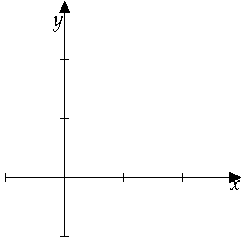
\includegraphics{plano-cartesiano.pdf}
	% \begin{tikzpicture}[line cap=round,line join=round,>=triangle 45,x=1.0cm,y=1.0cm]
	% 	\draw[->,color=black] (-1,0) -- (3,0);
	% 	\foreach \x in {-1,1,2}
	% 	\draw[shift={(\x,0)},color=black] (0pt,2pt) -- (0pt,-2pt);
	% 	\draw[color=black] (2.68,0.08) node [anchor=north west] {$x$};
	% 	\draw[->,color=black] (0,-1) -- (0,3);
	% 	\foreach \y in {-1,1,2}
	% 	\draw[shift={(0,\y)},color=black] (2pt,0pt) -- (-2pt,0pt);
	% 	\draw[color=black] (0.1,2.6) node [anchor=east] {$y$};
	% 	\clip(-1,-1) rectangle (3,3);
	% \end{tikzpicture}
\end{figure}


Seja $P$ um ponto qualquer do plano. Por $P$ podemos tra\c{c}ar uma \'unica reta $x'$ paralela \`a reta $x$ e uma \'unica reta $y'$ paralela \`a reta $y$. Estas retas interceptam $x$ e $y$ em pontos $P_x$ e $P_y$, respectivamente. Seja $\alpha$ o n\'umero real correspondente a $P_x$ e $\beta$ o n\'umero real correspondente  a $P_y$. Estes dois n\'umeros determinam o ponto $P$, isto \'e, conhecendo $\alpha$ e $\beta$ podemos tra\c{c}as as retas $x'$ e $y'$. O ponto $P$ \'e a interse\c{c}\~ao destas retas. Os n\'umeros $\alpha$ e $\beta$ s\~ao chamados \textbf{abscissa} e \textbf{ordenada} do ponto $P$, respectivamente. Eles constituem as \textbf{coordenadas} de $P$.
\begin{figure}[!h]
	\centering
	\caption{Coordenadas do ponto $P$}
	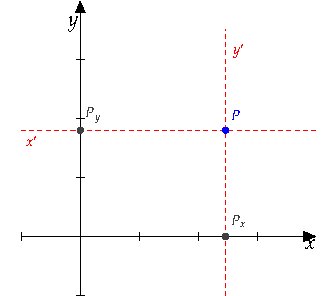
\includegraphics{coordenadas-plano-cartesiano.pdf}
	% \definecolor{uququq}{rgb}{0.25,0.25,0.25}
	% \definecolor{ffqqqq}{rgb}{1,0,0}
	% \definecolor{qqqqff}{rgb}{0,0,1}
	% \begin{tikzpicture}[line cap=round,line join=round,>=triangle 45,x=1.0cm,y=1.0cm]
	% 	\draw[->,color=black] (-1,0) -- (4,0);
	% 	\foreach \x in {-1,1,2,3}
	% 	\draw[shift={(\x,0)},color=black] (0pt,2pt) -- (0pt,-2pt);
	% 	\draw[color=black] (3.68,0.08) node [anchor=north west] {$x$};
	% 	\draw[->,color=black] (0,-1) -- (0,4);
	% 	\foreach \y in {-1,1,2,3}
	% 	\draw[shift={(0,\y)},color=black] (2pt,0pt) -- (-2pt,0pt);
	% 	\draw[color=black] (0.1,3.6) node [anchor=east] {$y$};
	% 	\clip(-1,-1) rectangle (4,4);
	% 	\draw [dash pattern=on 2pt off 2pt,color=ffqqqq] (2.46,-1) -- (2.46,3.5);
	% 	\draw [dash pattern=on 2pt off 2pt,color=ffqqqq,domain=-1:4] plot(\x,{(--1.8-0*\x)/1});
	% 	\begin{scriptsize}
	% 		\fill [color=qqqqff] (2.46,1.8) circle (1.5pt);
	% 		\draw[color=qqqqff] (2.62,2.06) node {$P$};
	% 		\draw[color=ffqqqq] (2.68,3.14) node {$y'$};
	% 		\draw[color=ffqqqq] (-0.82,1.62) node {$x'$};
	% 		\fill [color=uququq] (2.46,0) circle (1.5pt);
	% 		\draw[color=uququq] (2.68,0.26) node {$P_x$};
	% 		\fill [color=uququq] (0,1.8) circle (1.5pt);
	% 		\draw[color=uququq] (0.22,2.06) node {$P_y$};
	% 	\end{scriptsize}
	% \end{tikzpicture}
\end{figure}

Denotaremos assim o ponto $P$ por
\[
	P(\alpha,\beta).
\]

Sejam $P(x_1,y_1)$ e $Q(x_2,y_2)$ pontos do plano. A partir de $P$ e $Q$ podemos construir o tri\^angulo ret\^angulo $PQS$ como abaixo:
\begin{figure}[!h]
	\centering
	\caption{Dist\^ancia entre dois pontos}
	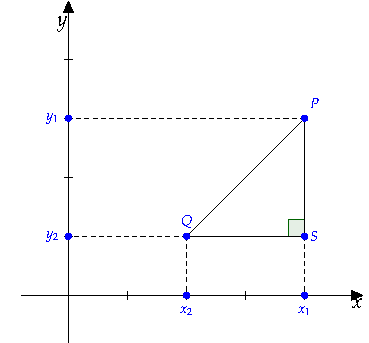
\includegraphics{distancia-pontos-plano-cartesiano.pdf}
	% \definecolor{qqwuqq}{rgb}{0,0.39,0}
	% \definecolor{xdxdff}{rgb}{0.49,0.49,1}
	% \definecolor{qqqqff}{rgb}{0,0,1}
	% \begin{tikzpicture}[line cap=round,line join=round,>=triangle 45,x=1.0cm,y=1.0cm]
	% 	\draw[->,color=black] (-0.8,0) -- (5,0);
	% 	\foreach \x in {,1,2,3,4}
	% 	\draw[shift={(\x,0)},color=black] (0pt,2pt) -- (0pt,-2pt);
	% 	\draw[color=black] (4.68,0.08) node [anchor=north west] {$x$};
	% 	\draw[->,color=black] (0,-0.8) -- (0,5);
	% 	\foreach \y in {,1,2,3,4}
	% 	\draw[shift={(0,\y)},color=black] (2pt,0pt) -- (-2pt,0pt);
	% 	\draw[color=black] (0.1,4.6) node [anchor=east] {$y$};
	% 	\clip(-0.8,-0.8) rectangle (5,5);
	% 	\draw[color=qqwuqq,fill=qqwuqq,fill opacity=0.1] (4,1.28) -- (3.72,1.28) -- (3.72,1) -- (4,1) -- cycle; 
	% 	\draw (4,1)-- (4,3);
	% 	\draw (2,1)-- (4,1);
	% 	\draw (2,1)-- (4,3);
	% 	\draw [dash pattern=on 2pt off 2pt] (4,3)-- (0,3);
	% 	\draw [dash pattern=on 2pt off 2pt] (2,1)-- (0,1);
	% 	\draw [dash pattern=on 2pt off 2pt] (2,1)-- (2,0);
	% 	\draw [dash pattern=on 2pt off 2pt] (4,1)-- (4,0);
	% 	\begin{scriptsize}
	% 		\fill [color=qqqqff] (2,1) circle (1.5pt);
	% 		\draw[color=qqqqff] (2,1.26) node {$Q$};
	% 		\fill [color=qqqqff] (4,3) circle (1.5pt);
	% 		\draw[color=qqqqff] (4.16,3.26) node {$P$};
	% 		\fill [color=qqqqff] (4,1) circle (1.5pt);
	% 		\draw[color=qqqqff] (4.16,1) node {$S$};
	% 		\fill [color=qqqqff] (0,3) circle (1.5pt);
	% 		\draw[color=qqqqff] (-0.28,3) node {$y_1$};
	% 		\fill [color=qqqqff] (0,1) circle (1.5pt);
	% 		\draw[color=qqqqff] (-0.28,1) node {$y_2$};
	% 		\fill [color=qqqqff] (2,0) circle (1.5pt);
	% 		\draw[color=qqqqff] (2,-0.26) node {$x_2$};
	% 		\fill [color=qqqqff] (4,0) circle (1.5pt);
	% 		\draw[color=qqqqff] (4,-0.26) node {$x_1$};
	% 	\end{scriptsize}
	% \end{tikzpicture}
\end{figure}

Assim sua hipotenusa \'e
\[
	\sqrt{(x_1 - x_2)^2 + (y_1 - y_2)^2}.
\]
Este n\'umero \'e chamado \textbf{dist\^ancia} de $P$ a $Q$ e \'e indicado por $d(P,Q)$, isto \'e, por defini\c{c}\~ao
\[
	d(P,Q) = \sqrt{(x_1 - x_2)^2 + (y_1 - y_2)^2}.
\]

Dizemos que dois pontos $P(x_1,y_1)$ e $Q(x_2,y_2)$ s\~ao iguais se, e somente se, $x_1 = x_2$ e $y_1 = y_2$.

% section plano_cartesiano (end)

\section{Vetores em $\real^2$} % (fold)
\label{sec:vetores_plano}

% Os vetores e as opera\c{c}\~ores com eles podem ser definidas utilizando-se do sistema de coordenadas cartesianas. Para isso, um ponto $P$ do plano \'e representado em $\real^2$ por um par de coordenadas $P(x_1, y_1)$, onde $x_1$, $y_1 \in \real$.

% Seja $\vec{u}$ um vetor no plano. Sabemos que $\vec{u}$ \'e um representante de uma certa classe de equipol\^encia dos segmentos orientados $(B,C)$. Para este segmento orientado $(B,C)$ podemos encontrar um ponto $A(x_1, y_1)$ tal que o segmento orientado $(O,A)$, onde $O(0,0)$, tem o mesmo comprimento, a mesma dire\c{c}\~ao e o mesmo sentido de $(B,C)$. Assim o vetor $\vec{u}$ pode ser representado pelo segmento orientado $(O,A)$. Portanto qualquer vetor em $\real^2$ pode ser representado como um segmento com origem no ponto $(0,0)$ e extremidade em um ponto $(x_1,y_1)$.

Sabemos que a cada par ordenado $(\alpha, \beta)$ corresponde um ponto do plano. Assim se $(\alpha, \beta) \ne (0,0)$ podemos associar uma seta com origem em $O(0,0)$ e extremidade em $(\alpha,\beta)$ como na figura abaixo:

\begin{figure}[!h]
	\centering
	\caption{Seta representando o ponto $(\alpha, \beta)$.}
	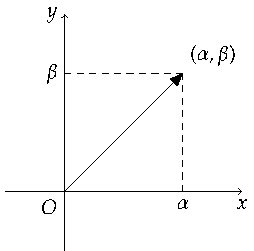
\includegraphics{vetores-plano-cartesiano.pdf}
 %  	\begin{tikzpicture}[scale=2]%vetor no plano
	%     \coordinate[label=below left:$O$] (A) at (0,0);
	%     \coordinate (W) at (1,1);
	%     %defini\c{c}\~ao das coordenadas dos eixos cartesianos
	%     \coordinate (F) at (-0.5,0);
	%     \coordinate (G) at (0,-0.5);
	%     \coordinate (X) at (1.5,0);
	%     \coordinate (Y) at (0,1.5);
	%     % Styles
	%     \tikzstyle{axes}=[]

	%     \begin{scope}[style=axes]%constr\'oi os eixos cartesianos
	% 	    \draw[->] (F) -- (X) node[below] {$x$} coordinate(x axis);
	% 	    \draw[->] (G) -- (Y) node[left] {$y$} coordinate(y axis);
	%     \end{scope}

	%     \draw[->,>=triangle 45] (A)--(W)
	%       node[above right]{$(\alpha, \beta)$};
	%     \draw[dashed,color=black] let \p1 = (W) in (\x1,0) -- (\x1,\y1)
	%       node[at start, below]{$\alpha$};
	%     \draw[dashed,color=black] let \p1 = (W) in (0,\y1) -- (\x1,\y1)
	%       node[at start, left]{$\beta$};
 %    \end{tikzpicture}
\end{figure}

Assim o par ordenado $(\alpha, \beta)$ pode ser representado graficamente por um ponto ou por uma seta. Quando representamos $(\alpha, \beta)$ por uma seta, podemos associar a este para uma \textbf{dire\c{c}\~ao}, um \textbf{sentido} e um \textbf{m\'odulo}. A dire\c{c}\~ao e o sentido do par $(\alpha, \beta)$ s\~ao respectivamente, a dire\c{c}\~ao e o sentido da seta que o representa. O \textbf{m\'odulo} do par $(\alpha, \beta)$ \'e o n\'umero
\[
	\sqrt{\alpha^2 + \beta^2}
\] 
que \'e o comprimento da seta.

Em geral, um objeto ao qual podemos associar os conceitos de dire\c{c}\~ao, sentido e m\'odulo \'e chamado um \textbf{vetor}. Denotaremos um vetor de extremidade em um ponto $(\alpha, \beta)$ por
\[
	\vec{u} = (\alpha, \beta).
\]

Esta nota\c{c}\~ao significa que $\vec{u}$ \'e a seta com in{\'\i}cio no ponto $O(0,0)$ e final no ponto $(\alpha, \beta)$.
\begin{figure}[!h]
	\centering
	\caption{Vetor $ \vec{u} = (\alpha, \beta)$.}
	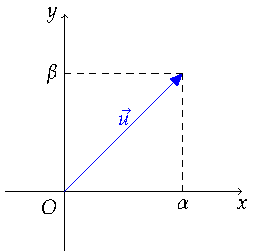
\includegraphics{vetor-coordenadas-plano-cartesiano.pdf}
  	% \begin{tikzpicture}[scale=2]%vetor no plano
	  %   \coordinate[label=below left:$O$] (A) at (0,0);
	  %   \coordinate (W) at (1,1);
	  %   %defini\c{c}\~ao das coordenadas dos eixos cartesianos
	  %   \coordinate (F) at (-0.5,0);
	  %   \coordinate (G) at (0,-0.5);
	  %   \coordinate (X) at (1.5,0);
	  %   \coordinate (Y) at (0,1.5);
	  %   % Styles
	  %   \tikzstyle{axes}=[]

	  %   \begin{scope}[style=axes]%constr\'oi os eixos cartesianos
		 %    \draw[->] (F) -- (X) node[below] {$x$} coordinate(x axis);
		 %    \draw[->] (G) -- (Y) node[left] {$y$} coordinate(y axis);
	  %   \end{scope}

	  %   \draw[->,>=triangle 45,color=blue] (A)--(W)
	  %     node[midway, above]{$\vec{u}$};
	  %   \draw[dashed,color=black] let \p1 = (W) in (\x1,0) -- (\x1,\y1)
	  %     node[at start, below]{$\alpha$};
	  %   \draw[dashed,color=black] let \p1 = (W) in (0,\y1) -- (\x1,\y1)
	  %     node[at start, left]{$\beta$};
   %  \end{tikzpicture}
\end{figure}

% Assim escrevemos $\vec{u} = \vec{OP}$. Para simplificar a nota\c{c}\~ao vamos identificar o vetor $\vec{u} = \vec{OP}$ com as coordenadas de sua extremidade e da{\'\i} escrevemos
% \[
%   \vec{u} = (x_1,y_1).
% \]
% As coordenadas $(x_1,y_1)$ s\~ao chamadas de \textbf{componentes} do vetor $\vec{u}$. Com essa representa\c{c}\~ao, o vetor nulo $\vec{0}$ \'e escrito como
% \[
%   \vec{0} = (0,0).
% \]

Por exemplo, $\vec{u} = (3,2)$ e $\vec{v} = (-1,-2)$ s\~ao representados graficamente por:
\begin{figure}[!h]
	\centering
	\caption{Vetores $\vec{u} = (3,2)$ e $\vec{v} = (-1,-2)$.}
	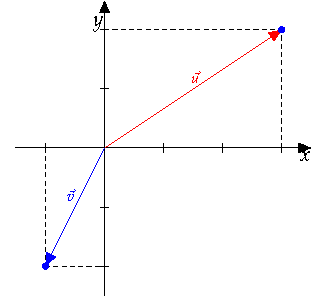
\includegraphics{exemplo-vetores-plano-cartesiano.pdf}
	% \definecolor{ffqqqq}{rgb}{1,0,0}
	% \definecolor{qqqqff}{rgb}{0,0,1}
	% \begin{tikzpicture}[line cap=round,line join=round,>=triangle 45,x=1.0cm,y=1.0cm]
	% 	\draw[->,color=black] (-1.5,0) -- (3.5,0);
	% 	\foreach \x in {-1,1,2,3}
	% 	\draw[shift={(\x,0)},color=black] (0pt,2pt) -- (0pt,-2pt);
	% 	\draw[color=black] (3.18,0.08) node [anchor=north west] {$x$};
	% 	\draw[->,color=black] (0,-2.5) -- (0,2.5);
	% 	\foreach \y in {-2,-1,1,2}
	% 	\draw[shift={(0,\y)},color=black] (2pt,0pt) -- (-2pt,0pt);
	% 	\draw[color=black] (0.1,2.1) node [anchor=east] {$y$};
	% 	\clip(-1.5,-2.5) rectangle (3.5,2.5);
	% 	\draw [->,color=ffqqqq] (0,0) -- (3,2);
	% 	\draw [->,color=qqqqff] (0,0) -- (-1,-2);
	% 	\draw [dash pattern=on 2pt off 2pt] (3,0)-- (3,2);
	% 	\draw [dash pattern=on 2pt off 2pt] (0,2)-- (3,2);
	% 	\draw [dash pattern=on 2pt off 2pt] (-1,0)-- (-1,-2);
	% 	\draw [dash pattern=on 2pt off 2pt] (-1,-2)-- (0,-2);
	% 	\begin{scriptsize}
	% 		\fill [color=qqqqff] (3,2) circle (1.5pt);
	% 		%\draw[color=qqqqff] (3.16,2.26) node {$A$};
	% 		\fill [color=qqqqff] (-1,-2) circle (1.5pt);
	% 		%\draw[color=qqqqff] (-1.16,-2.2) node {$B$};
	% 		\draw[color=ffqqqq] (1.54,1.2) node {$\vec{u}$};
	% 		\draw[color=qqqqff] (-0.58,-0.8) node {$\vec{v}$};
	% 	\end{scriptsize}
	% \end{tikzpicture}
\end{figure}

O vetor que tem in{\'\i}cio e fim no ponto $(0,0)$ \'e chamado de \textbf{vetor nulo} e ser\'a denotado por
\[
	\vec{O} = (0,0).
\]

Podemos tamb\'em representar um vetor por uma seta que n\~ao parte da origem. Por exemplo, os pontos $A(x_1,y_1)$ e $B(x_2,y_2)$ determinam o vetor
\[
	\vec{AB} = (x_2 - x_1, y_2 - y_1).
\]
\begin{figure}[!h]
	\centering
	\caption{Vetor $\vec{AB}$}
	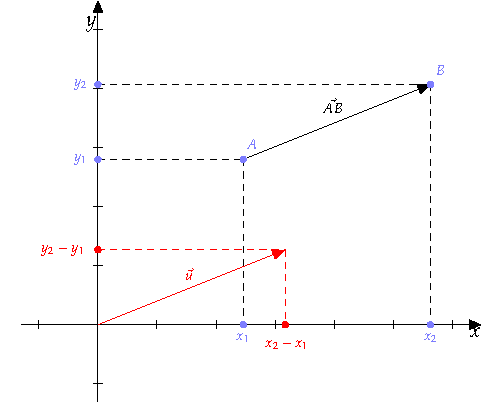
\includegraphics{vetor-AB-plano-cartesiano.pdf}
	% \definecolor{uququq}{rgb}{0.25,0.25,0.25}
	% \definecolor{ffqqqq}{rgb}{1,0,0}
	% \definecolor{xdxdff}{rgb}{0.49,0.49,1}
	% \begin{tikzpicture}[line cap=round,line join=round,>=triangle 45,x=1.0cm,y=1.0cm]
	% 	\draw[->,color=black] (-1.3,0) -- (6.5,0);
	% 	\foreach \x in {-1,1,2,3,4,5,6}
	% 	\draw[shift={(\x,0)},color=black] (0pt,2pt) -- (0pt,-2pt);
	% 	\draw[color=black] (6.18,0.08) node [anchor=north west] {$x$};
	% 	\draw[->,color=black] (0,-1.3) -- (0,5.5);
	% 	\foreach \y in {-1,1,2,3,4,5}
	% 	\draw[shift={(0,\y)},color=black] (2pt,0pt) -- (-2pt,0pt);
	% 	\draw[color=black] (0.1,5.1) node [anchor=east] {$y$};
	% 	\clip(-1.3,-1.3) rectangle (6.5,5.5);
	% 	\draw [->] (2.46,2.8) -- (5.63,4.07);
	% 	\draw [->,color=ffqqqq] (0,0) -- (3.17,1.27);
	% 	\draw [dash pattern=on 3pt off 3pt] (0,2.8)-- (2.46,2.8);
	% 	\draw [dash pattern=on 3pt off 3pt] (0,4.07)-- (5.63,4.07);
	% 	\draw [dash pattern=on 3pt off 3pt] (5.63,4.07)-- (5.63,0);
	% 	\draw [dash pattern=on 3pt off 3pt] (2.46,2.8)-- (2.46,0);
	% 	\draw [dash pattern=on 3pt off 3pt,color=ffqqqq] (0,1.27)-- (3.17,1.27);
	% 	\draw [dash pattern=on 3pt off 3pt,color=ffqqqq] (3.17,1.27)-- (3.17,0);
	% 	\begin{scriptsize}
	% 		\fill [color=xdxdff] (5.63,4.07) circle (1.5pt);
	% 		\draw[color=xdxdff] (5.8,4.32) node {$B$};
	% 		\draw[color=black] (3.98,3.72) node {$\vec{AB}$};
	% 		\draw[color=ffqqqq] (1.54,0.86) node {$\vec{u}$};
	% 		\fill [color=xdxdff] (2.46,2.8) circle (1.5pt);
	% 		\draw[color=xdxdff] (2.62,3.06) node {$A$};
	% 		\fill [color=xdxdff] (0,2.8) circle (1.5pt);
	% 		\draw[color=xdxdff] (-0.3,2.8) node {$y_1$};
	% 		\fill [color=xdxdff] (0,4.07) circle (1.5pt);
	% 		\draw[color=xdxdff] (-0.3,4.07) node {$y_2$};
	% 		\fill [color=xdxdff] (2.46,0) circle (1.5pt);
	% 		\draw[color=xdxdff] (2.46,-0.22) node {$x_1$};
	% 		\fill [color=xdxdff] (5.63,0) circle (1.5pt);
	% 		\draw[color=xdxdff] (5.63,-0.22) node {$x_2$};
	% 		\fill [color=ffqqqq] (3.17,0) circle (1.5pt);
	% 		\draw[color=ffqqqq] (3.2,-0.32) node {$x_2-x_1$};
	% 		\fill [color=ffqqqq] (0,1.27) circle (1.5pt);
	% 		\draw[color=ffqqqq] (-0.6,1.27) node {$y_2-y_1$};
	% 	\end{scriptsize}
	% \end{tikzpicture}
\end{figure}

Assim a seta que representa o vetor $\vec{AB}$ e a seta que representa o vetor $\vec{u}$, que tem in{\'\i}cio na origem e extremidade no ponto $(x_2 - x_1, y_2 - y_1)$, t\^em o mesmo m\'odulo, dire\c{c}\~ao e sentido que $\vec{AB}$. Assim vamos representar o vetor $\vec{AB}$ pela forma que for mais conveniente.

\begin{definicao}
  Seja $\vec{u} = (x_1, y_1)$ um vetor. A \textbf{norma} de $\vec{u}$, denotada por $\norm{\vec{u}}$, \'e dada por
  \[
    \norm{\vec{u}} = \sqrt{x_1^2 + y_1^2}.
  \]
\end{definicao}

Um vetor $\vec{u}$ tal que
\[
	\norm{\vec{u}} = 1
\]
\'e chamado de \textbf{vetor unit\'ario}.
\begin{figure}[!h]
	\centering
	\caption{Vetores unit\'arios: $\norm{\vec{u}} = 1$}
	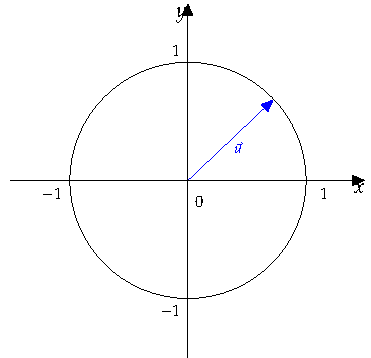
\includegraphics{vetores-unitarios-plano-cartesiano.pdf}
	% \definecolor{qqqqff}{rgb}{0,0,1}
	% \begin{tikzpicture}[line cap=round,line join=round,>=triangle 45,x=1.0cm,y=1.0cm]
	% 	\draw[->,color=black] (-3,0) -- (3,0);
	% 	\draw (-2.3,0) node[below] {\footnotesize $-1$};
	% 	\draw (2.3,0) node[below] {\footnotesize $1$};
	% 	\draw (0,2.2) node[left] {\footnotesize $1$};
	% 	\draw (0,-2.2) node[left] {\footnotesize $-1$};
	% 	\draw[color=black] (2.68,0.08) node [anchor=north west] {$x$};
	% 	\draw[->,color=black] (0,-3) -- (0,3);
	% 	\draw[color=black] (0.1,2.8) node [anchor=east] {$y$};
	% 	\draw[color=black] (0pt,-10pt) node[right] {\footnotesize $0$};
	% 	\clip(-3,-3) rectangle (3,3);
	% 	\draw(0,0) circle (2cm);
	% 	\draw [->,color=qqqqff] (0,0) -- (1.45,1.37);
	% 	\begin{scriptsize}
	% 		\draw[color=qqqqff] (0.84,0.56) node {$\vec{u}$};
	% 	\end{scriptsize}
	% \end{tikzpicture}
\end{figure}

\begin{definicao}
	Dois vetores $\vec{u}$ e $\vec{v}$ s\~ao \textbf{paralelos} (ou \textbf{colineares}) se a restas que cont\'em estes vetores s\~ao paralelas(podendo ser coincidentes).Caso $\vec{u}$ e $\vec{v}$ sejam paralelos, escreveremos $\vec{u}\varparallel\vec{v}$. Neste caso, $\vec{u}$ e $\vec{v}$ t\^em a mesma dire\c{c}\~ao, mas podem ter sentidos contr\'arios.
\end{definicao}
\begin{figure}[!h]
	\centering
	\caption{Vetores paralelos}
	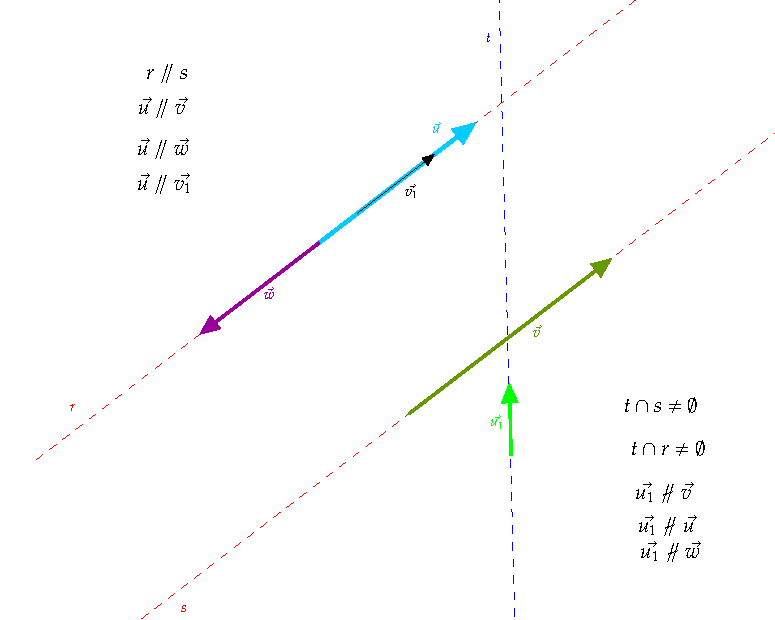
\includegraphics{vetores-paralelos-plano-cartesiano.pdf}
	% \definecolor{qqffqq}{rgb}{0,1,0}
	% \definecolor{qqqqff}{rgb}{0,0,1}
	% \definecolor{zzqqzz}{rgb}{0.6,0,0.6}
	% \definecolor{wwzzqq}{rgb}{0.4,0.6,0}
	% \definecolor{qqccff}{rgb}{0,0.8,1}
	% \definecolor{ffqqqq}{rgb}{1,0,0}
	% \begin{tikzpicture}[line cap=round,line join=round,>=triangle 45,x=1.0cm,y=1.0cm]
	% 	\clip(-3.5,-4.5) rectangle (9,6);
	% 	\draw [dash pattern=on 4pt off 4pt,color=ffqqqq,domain=-3.5:9] plot(\x,{(--2.39--2.04*\x)/2.66});
	% 	\draw [dash pattern=on 4pt off 4pt,color=ffqqqq,domain=-3.5:9] plot(\x,{(-8.41--2.04*\x)/2.66});
	% 	\draw [->,line width=1.6pt,color=qqccff] (1.28,1.88) -- (3.94,3.92);
	% 	\draw [->,line width=1.2pt,color=wwzzqq] (2.82,-1) -- (6.24,1.62);
	% 	\draw [->,line width=1.2pt,color=zzqqzz] (1.28,1.88) -- (-0.73,0.34);
	% 	\draw [dash pattern=on 4pt off 4pt,color=qqqqff,domain=-3.5:9] plot(\x,{(--8.89-1.98*\x)/0.05});
	% 	\draw [->,line width=1.2pt,color=qqffqq] (4.54,-1.7) -- (4.51,-0.49);
	% 	\draw [->] (1.94,2.39) -- (3.25,3.39);
	% 	\draw (-1.76,5.04) node[anchor=north west] {$ r\varparallel s $};
	% 	\draw (-1.9,4.48) node[anchor=north west] {$\vec{u}\varparallel \vec{v}$};
	% 	\draw (-1.92,3.78) node[anchor=north west] {$\vec{u}\varparallel \vec{w}$};
	% 	\draw (-1.92,3.2) node[anchor=north west] {$\vec{u}\varparallel \vec{v_1}$};
	% 	\draw (6.32,-0.6) node[anchor=north west] {$ t \cap s \ne \emptyset $};
	% 	\draw (6.44,-1.32) node[anchor=north west] {$ t \cap r \ne \emptyset $};
	% 	\draw (6.52,-2.04) node[anchor=north west] {$\vec{u_1}\nvarparallel \vec{v}$};
	% 	\draw (6.56,-2.6) node[anchor=north west] {$\vec{u_1}\nvarparallel \vec{u}$};
	% 	\draw (6.6,-3.04) node[anchor=north west] {$\vec{u_1}\nvarparallel \vec{w}$};
	% 	\begin{scriptsize}
	% 		\draw[color=ffqqqq] (-2.88,-0.9) node {$r$};
	% 		\draw[color=ffqqqq] (-1,-4.3) node {$s$};
	% 		\draw[color=qqccff] (3.26,3.84) node {$\vec{u}$};
	% 		\draw[color=wwzzqq] (4.98,0.4) node {$\vec{v}$};
	% 		\draw[color=zzqqzz] (0.44,1.04) node {$\vec{w}$};
	% 		\draw[color=qqqqff] (4.16,5.36) node {$t$};
	% 		\draw[color=qqffqq] (4.3,-1.14) node {$\vec{u_1}$};
	% 		\draw[color=black] (2.86,2.76) node {$\vec{v_1}$};
	% 	\end{scriptsize}
	% \end{tikzpicture}
\end{figure}

\subsection{Opera\c{c}\~oes com Vetores} % (fold)
\label{sub:operacoes_com_vetores}

\begin{definicao}
  Sejam $\vec{u} = (x_1, y_1)$ e $\vec{v} = (x_2, y_2)$ vetores. Ent\~ao:
  \[
  	\vec{u} + \vec{v} = (x_1 + x_2, y_1 + y_2).
  \]
\end{definicao}

\begin{figure}[!h]
  \centering
  \caption{Soma de vetores}
  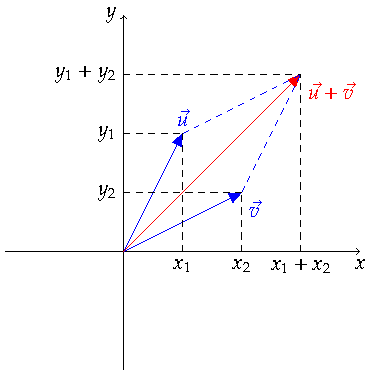
\includegraphics{soma-vetores-plano-cartesiano.pdf}
  % \begin{tikzpicture}[scale=2]%soma de vetores no plano
  %   \coordinate (A) at (0,0);
  %   \coordinate (V) at (0.5,1);
  %   \coordinate (W) at (1,0.5);
  %   \coordinate (B) at (0,1);
  %   \coordinate (VW) at ($(V)+(W)$);
  %   %defini\c{c}\~ao das coordenadas dos eixos cartesianos
  %   \coordinate (F) at (-1,0);
  %   \coordinate (G) at (0,-1);
  %   \coordinate (X) at (2,0);
  %   \coordinate (Y) at (0,2);
  %   % Styles
  %   \tikzstyle{axes}=[]

  %   \begin{scope}[style=axes]%constr\'oi os eixos cartesianos
  %   \draw[->] (F) -- (X) node[below] {$x$} coordinate(x axis);
  %   \draw[->] (G) -- (Y) node[left] {$y$} coordinate(y axis);
  %   \end{scope}

  %   \draw[->,>=triangle 45,color=blue] (A)--(V)
  %     node[above]{$\vec{u}$};
  %   \draw[->,>=triangle 45,color=blue] (A)--(W)
  %     node[below right]{$\vec{v}$};
  %   \draw[->,>=triangle 45,color=red] (A)--(VW)
  %     node[below right]{$\vec{u}+\vec{v}$};
  %   \draw[dashed,>=triangle 45,color=blue] (V)--(VW);
  %   \draw[dashed,>=triangle 45,color=blue] (W)--(VW);
  %   \draw[dashed,color=black] let \p1 = (V) in (\x1,0) -- (\x1,\y1)
  %     node[at start, below]{$x_1$};
  %   \draw[dashed,color=black] let \p1 = (V) in (0,\y1) -- (\x1,\y1)
  %     node[at start, left]{$y_1$};
  %   \draw[dashed,color=black] let \p1 = (W) in (\x1,0) -- (\x1,\y1)
  %     node[at start, below]{$x_2$};
  %   \draw[dashed,color=black] let \p1 = (W) in (0,\y1) -- (\x1,\y1)
  %     node[at start, left]{$y_2$};
  %   \draw[dashed,color=black] let \p1 = (VW) in (\x1,0) -- (\x1,\y1)
  %     node[at start, below]{$x_1 + x_2$};
  %   \draw[dashed,color=black] let \p1 = (VW) in (0,\y1) -- (\x1,\y1)
  %     node[at start, left]{$y_1 + y_2$};
  % \end{tikzpicture}
\end{figure}

\begin{propriedades}\label{propriedades_soma_vetores}
  Sejam $\vec{u}$, $\vec{v}$ e $\vec{w}$ vetores quaisquer. As seguintes propriedades s\~ao verdadeiras:
  \begin{enumerate}[label=({\roman*})]
    \item $(\vec{u} + \vec{v}) + \vec{w} = \vec{u} + (\vec{v} + \vec{w})$ [Associatividade]
    \item $\vec{u} + \vec{v} = \vec{v} + \vec{u}$ [Comutatividade]
    \item Existe um \'unico vetor que somado a $\vec{u}$ resulta no pr\'oprio vetor $\vec{u}$:
    \[
      \vec{u} + \vec{0} = \vec{0} + \vec{u} = \vec{u}.
    \]
    Tal vetor \'e o vetor nulo. [Elementro Neutro]
    \item\label{vetor_oposto} Para cada $\vec{u}$, existe um \'unico vetor $\vec{v}$ tal que
    \[
      \vec{u} + \vec{v} = \vec{0} = \vec{v} + \vec{u}.
    \]
    O vetor $\vec{v}$ \'e o vetor oposto de $\vec{u}$. [Elemento Oposto]
  \end{enumerate}
\end{propriedades}
\begin{prova}
	Sejam $\vec{u} = (x_1,y_1)$, $\vec{v} = (x_2,y_2)$ e $\vec{w} = (x_3,y_3)$. Temos
	\begin{enumerate}[label=({\roman*})]
		\item $(\vec{u} + \vec{v}) + \vec{w} = (x_1+x_2,y_1+y_2) + \vec{w} = ((x_1+x_2)+x_3,(y_1+y_2)+y_3) = (x_1+(x_2+x_3),y_1+(y_2+y_3)) = \vec{u} + (x_2+x_3,y_2+y_3) = \vec{u} + (\vec{v} + \vec{w})$.
		\item $\vec{u} + \vec{v} = (x_1+x_2,y_1+y_2) = (x_2+x_1,y_2+y_1) = \vec{v} + \vec{u}$.
		\item Usando o item (A2) basta verificar que $\vec{u} + \vec{0} = \vec{u}$. De fato
		\[
      		\vec{u} + \vec{0} = (x_1,y_1) + (0,0) = (x_1,y_1) = \vec{u}.
    	\]
    	\item Novamente, pelo item (A2) basta verificar que $\vec{u} + \vec{v} = \vec{0}$. De fato, dado $\vec{u} = (x_1,y_1)$, tomando $\vec{v} = (-x_1,-y_1)$ temos
    	\[
    		\vec{u} + \vec{v} = (x_1,y_1) + (-x_1,-y_1) = (0,0) = \vec{0}.
    	\]
	\end{enumerate}
	Portanto as propriedades s\~ao verdadeiras.
\end{prova}

\begin{definicao}
	O vetor $\vec{v}$ do item \ref{vetor_oposto} da Defini\c{c}\~ao \ref{propriedades_soma_vetores} \'e chamado de \textbf{vetor oposto}.
\end{definicao}


\begin{definicao}
  Sejam $\alpha \in \real$, $\vec{u} = (x_1, y_1)$ e $\vec{v} = (x_2, y_2)$ vetores. Ent\~ao:
  \[
  	\alpha \vec{u} = (\alpha x_1, \alpha y_1).
  \]
\end{definicao}

\begin{figure}[!h]
  \centering
  \caption{Multiplica\c{c}\~ao por escalar}
  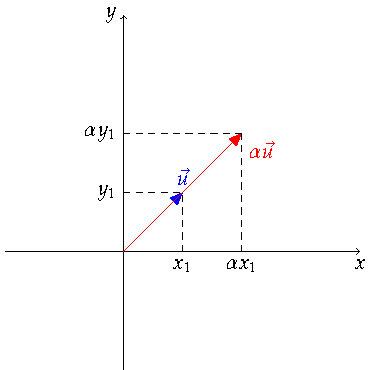
\includegraphics{multiplicacao-escalar-vetores-plano-cartesiano.pdf}
  % \begin{tikzpicture}[scale=2]%multiplica\c{c}\~ao por escalar no plano
  %   \coordinate (A) at (0,0);
  %   \coordinate (V) at (0.5,0.5);
  %   \coordinate (W) at ($2*(V)$);
  %   %defini\c{c}\~ao das coordenadas dos eixos cartesianos
  %   \coordinate (F) at (-1,0);
  %   \coordinate (G) at (0,-1);
  %   \coordinate (X) at (2,0);
  %   \coordinate (Y) at (0,2);
  %   % Styles
  %   \tikzstyle{axes}=[]

  %   \begin{scope}[style=axes]%constr\'oi os eixos cartesianos
	 %    \draw[->] (F) -- (X) node[below] {$x$} coordinate(x axis);
	 %    \draw[->] (G) -- (Y) node[left] {$y$} coordinate(y axis);
  %   \end{scope}

  %   \draw[->,>=triangle 45,color=blue] (A)--(V)
  %     node[above]{$\vec{u}$};
  %   \draw[->,>=triangle 45,color=red] (A)--(W)
  %     node[below right]{$\alpha \vec{u}$};
  %   \draw[dashed,color=black] let \p1 = (V) in (\x1,0) -- (\x1,\y1)
  %     node[at start, below]{$x_1$};
  %   \draw[dashed,color=black] let \p1 = (V) in (0,\y1) -- (\x1,\y1)
  %     node[at start, left]{$y_1$};
  %   \draw[dashed,color=black] let \p1 = (W) in (\x1,0) -- (\x1,\y1)
  %     node[at start, below]{$\alpha x_1$};
  %   \draw[dashed,color=black] let \p1 = (W) in (0,\y1) -- (\x1,\y1)
  %     node[at start, left]{$\alpha y_1$};
  % \end{tikzpicture}
\end{figure}

\begin{observacao}
	\begin{enumerate}
		\item Sejam $\vec{u}$ um vetor n\~ao-nulo e $\lambda \ne 0$ um escalar. Ent\~ao $\vec{u} \varparallel\lambda\vec{u}$. Al\'em disso, se $\lambda > 0$, ent\~ao $\vec{u}$ e $\lambda\vec{u}$ s\~ao de mesmo sentido, e se $\lambda < 0$ ent\~ao $\vec{u}$ e $\lambda\vec{u}$ s\~ao de sentidos contr\'arios.
		\item Quando $\lambda = -1$, o vetor $-\vec{u} = (-x_1,-y_1)$  \'e exatamente o vetor oposto de $\vec{u}$. Note que $-\vec{u}$ tem a mesma dire\c{c}\~ao que $\vec{u}$, mas sentido contr\'ario.
	\end{enumerate}
	
\end{observacao}

\begin{propriedades}
  Quaisquer que sejam os n\'umeros reais $\alpha$ e $\beta$ e quaisquer que sejam os vetores $\vec{u}$ e $\vec{v}$ valem as igualdades:
  \begin{enumerate}[label=({\roman*})]
    \item $\alpha(\vec{u} + \vec{v}) = \alpha\vec{u} + \alpha\vec{v}$;
    \item $(\alpha + \beta)\vec{u} = \alpha\vec{u} + \beta\vec{u}$;
    \item $1\vec{u} = \vec{u}$;
    \item $\alpha(\beta\vec{u}) = (\alpha\beta)\vec{u} = \beta(\alpha\vec{u})$.
  \end{enumerate}
\end{propriedades}
\begin{prova}
	Sejam $\vec{u} = (x_1,y_1)$ e $\vec{v} = (x_2,y_2)$. Temos:
	\begin{enumerate}[label=({\roman*})]
		\item $\alpha(\vec{u} + \vec{v}) = \alpha(x_1+x_2,y_1+y_2) = (\alpha(x_1+x_2),\alpha(y_1+y_2)) = (\alpha x_1,\alpha y_1) + (\alpha x_2,\alpha y_2) =  \alpha\vec{u} + \alpha\vec{v}$.
		\item $(\alpha + \beta)\vec{u} = ((\alpha+\beta)x_1,(\alpha+\beta)y_1) = (\alpha x_1 + \beta x_1, \alpha y_1 + \beta y_1) = (\alpha x_1,\alpha y_1) + (\beta x_1,\beta y_1) = \alpha\vec{u} + \beta\vec{u}$.
		\item $1\vec{u} = 1(x_1,y_1) = (x_1,y_1) = \vec{u}$.
		\item Primeiro temos:
		\[
			\alpha(\beta\vec{u}) = \alpha(\beta x_1,\beta y_1) = (\alpha(\beta x_1),\alpha(\beta y_1)) = ((\alpha\beta)x_1,(\alpha\beta)y_1) = (\alpha\beta)\vec{u}.
		\]
		Agora,
		\[
			(\alpha\beta)\vec{u} = 	((\alpha\beta)x_1,(\alpha\beta)y_1) = ((\beta\alpha)x_1,(\beta\alpha)y_1) = (\beta(\alpha x_1),\beta(\alpha y_1)) = \beta(\alpha\vec{u}).
		\]
		Logo $\alpha(\beta\vec{u}) = (\alpha\beta)\vec{u} = \beta(\alpha\vec{u})$.
	\end{enumerate}
	Portanto as propriedades s\~ao v\'alidas.
\end{prova}

% \begin{proposicao}
%   Quaisquer que sejam o escalar $\alpha$ e o vetor $\vec{u}$, valem as seguintes igualdades:
%   \begin{enumerate}[label=({\roman*})]
%     \item $(-\alpha)\vec{u} = -(\alpha\vec{u})$;
%     \item $\alpha(-\vec{u}) = -(\alpha\vec{u})$;
%     \item $(-\alpha)(-\vec{u}) = \alpha\vec{u}$.
%   \end{enumerate}
% \end{proposicao}

Em alguns casos pode ser mais conveniente representar um vetor $\vec{u} = (x_1, y_1)$ de forma matricial. Para isso escrevemos as componentes de $\vec{u}$ como uma matriz de 1 coluna e duas linhas
\[
  \vec{u} = \begin{bmatrix}
    x_1\\y_1
  \end{bmatrix}.
\]

%Vimos que a norma de um vetor \'e definida como o comprimento de um segmento orientado que o represente. Com a representa\c{c}\~ao de vetores por coordenadas podemos reescrever o conceito de norma da seguinte maneira:

\begin{exemplos}
  Seja $\vec{u} = (-2,3)$ um vetor. Ent\~ao
  \begin{align*}
    \norm{\vec{u}} &= \sqrt{(-2)^2 + 3^2} = \sqrt{13}\\
    \vec{v} &= \dfrac{\vec{u}}{\norm{u}} = \dfrac{1}{\sqrt{13}}(-2,3) = \left(\dfrac{-2}{\sqrt{13}}, \dfrac{3}{\sqrt{13}}\right).
  \end{align*}
\end{exemplos}


% subsection operacoes_com_vetores (end)


% section vetores_plano (end)

\begin{proposicao}
  Sejam $\vec{u} = (x_1, y_1)$ um vetor em $\real^2$ e $\alpha \in \real$. Ent\~ao:
  \begin{enumerate}
    \item Se $\vec{u} \ne \vec{0}$, ent\~ao $\norm{\vec{u}} \ne 0$.
    \item $\norm{\vec{u}} = 0$ se, e somente se, $\vec{u} = \vec{0}$.
    \item $\norm{\alpha\vec{u}} = |\alpha|\norm{\vec{u}}$.
  \end{enumerate}
\end{proposicao}
\begin{prova}
  \begin{enumerate}
    \item  Se $\vec{u} \ne (0,0) = \vec{0}$, ent\~ao $x_1 \ne 0$ ou $y_1 \ne 0$. Da{\'\i}
    \[
      \norm{\vec{u}} = \sqrt{x_1^2 + y_1^2} > 0.
    \]
    \item $\norm{\vec{u}} = 0$ se, e somente se, $x_1^2 + y_1^2 = 0$, isto \'e, $x_1 = y_1 = 0$. Portanto $\vec{u} = \vec{0}$.
    \item $\norm{\alpha\vec{u}} = \norm{\alpha(x_1, y_1)} = \sqrt{(\alpha x_1)^2 + (\alpha y_1)^2} = \sqrt{\alpha^2(x_1^2 + y_1^2)} = |\alpha|\norm{\vec{u}}$.
  \end{enumerate}
\end{prova}

\begin{observacao}
	Dado um vetor n\~ao nulo $\vec{u}$ o vetor
	\[
  		\vec{v} = \dfrac{\vec{u}}{\norm{\vec{u}}}
	\]
	\'e um vetor unit\'ario na dire\c{c}\~ao de $\vec{u}$ pois
	\[
  		\norm{\vec{v}} = \norm{\dfrac{\vec{u}}{\norm{\vec{u}}}} = \dfrac{1}{\norm{\vec{u}}}\norm{\vec{u}} = 1.
	\]

\end{observacao}
\begin{definicao}
	Sejam $\vec{u}$ e $\vec{v}$ vetores n\~ao-nulos. Ent\~ao $\vec{u} = \vec{v}$ se, e somente se, $\vec{u}$ e $\vec{v}$ t\^em normas iguais, s\~ao de mesma dire\c{c}\~ao e de mesmo sentido.
\end{definicao}

\begin{proposicao}\label{vetores_paralelos}
  Dois vetores n\~ao nulos $\vec{u}$ e $\vec{v}$ s\~ao paralelos se, e somente se, existe um escalar $\lambda$ tal que $\vec{u} = \lambda\vec{v}$ (consequentemente, $\lambda \ne 0$ e assim $\vec{v} = \vec{u}/\lambda$).
\end{proposicao}
\begin{prova}
	Se $\vec{u} = \lambda\vec{v}$, ent\~ao $\vec{u}\varparallel\vec{v}$.
	Agora, suponha que $\vec{u}$ e $\vec{v}$ s\~ao paralelos e de mesmo sentido, o caso em que t\^em sentidos contr\'arios fica como exerc{\'\i}cio.

	Seja 
	\[
		\lambda = \dfrac{\norm{\vec{u}}}{\norm{\vec{v}}}.
	\]
	Vamos mostrar que $\vec{u} = \lambda\vec{v}$. Inicialmente, sabemos que $\vec{v}$ e $\lambda\vec{v}$ s\~ao paralelos e t\^em o mesmo sentido pois $\lambda > 0$. Agora
	\[
		\norm{\lambda\vec{v}} = |\lambda|\norm{\vec{v}} = \dfrac{\norm{\vec{u}}}{\norm{\vec{v}}}\norm{\vec{v}} = \norm{\vec{u}}.
	\]
	Portanto $\vec{u}$ e $\lambda\vec{v}$ tem a mesma dire\c{c}\~ao, o mesmo sentido e normas iguais, logo $\vec{u} = \lambda\vec{v}$, como quer{\'\i}amos.
\end{prova}

\subsection{\^Angulo entre vetores e produto interno} % (fold)
\label{sub:angulo_entre_vetores_e_produto_interno}
\begin{definicao}
  Sejam $\vec{u}$ e $\vec{v}$ vetores n\~ao nulos. O \textbf{\^angulo} entre $\vec{u}$ e $\vec{v}$ \'e definido pelo \^angulo $\theta$ determinado por $\vec{u}$ e $\vec{v}$ e que satisfaz $0 \le \theta \le \pi$, quando os vetores $\vec{u}$ e $\vec{v}$ s\~ao representados com a mesma origem.\index{Vetores!\^Angulo}
\end{definicao}

\begin{figure}[!h]
  \centering
  \caption{\^Angulo entre vetores}
  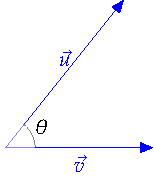
\includegraphics{angulo-vetores-plano-cartesiano.pdf}
  % \begin{tikzpicture}
  %   \coordinate (A) at (0,0);
  %   \coordinate (X) at (2.5,0);
  %   \coordinate (Y) at (2,2.5);

  %   \draw[->,>=triangle 45,color=blue] (A) -- (X)
  %     node[midway,below]{$\vec{v}$};
  %   \draw[->,>=triangle 45,color=blue] (A) -- (Y)
  %     node[midway,above]{$\vec{u}$};
  % % \draw[dashed,->,>=triangle 45] (X) -- (Y)
  %   % node[midway,above right]{$\vec{u} - \vec{v}$};

  %   % Mark the angle XAY
  %   \begin{scope}
  %     \path[clip] (A) -- (X) -- (Y);
  %     \fill[white, opacity=0.5, draw=black] (A) circle (5mm);
  %     \node at ($(A)+(30:7mm)$) {$\theta$};
  %   \end{scope}
  % \end{tikzpicture}
\end{figure}


\begin{definicao}
  Quando o \^angulo $\theta$ entre dois vetores $\vec{u}$ e $\vec{v}$ \'e reto, isto \'e, $\theta = \pi/2$, ou um deles \'e o vetor nulo, dizemos que os vetores $\vec{u}$ e $\vec{v}$ s\~ao \textbf{ortogonais} ou \textbf{perpendiculares} entre si. Denotamos tal fato, escrevendo $\vec{u} \perp \vec{v}$.\index{Vetores!Ortogonais}
\end{definicao}

Sejam $\vec{u}$ e $\vec{v}$ vetores n\~ao nulos e $\theta$ o \^angulo entre eles.
\begin{figure}[!h]
  \centering
  \caption{Determina\c{c}\~ao de $\theta$}
  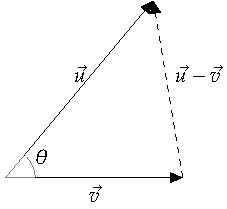
\includegraphics{determinacao-angulo-vetores-plano-cartesiano.pdf}
  % \begin{tikzpicture}
  %   \coordinate (A) at (0,0);
  %   \coordinate (X) at (3,0);
  %   \coordinate (Y) at (2.5,3);

  %   \draw[->,>=triangle 45] (A) -- (X)
  %   node[midway,below]{$\vec{v}$};
  %   \draw[->,>=triangle 45] (A) -- (Y)
  %   node[midway,above]{$\vec{u}$};
  %   \draw[dashed,->,>=triangle 45] (X) -- (Y)
  %   node[midway,above right]{$\vec{u} - \vec{v}$};

  %   % Mark the angle XAY
  %   \begin{scope}
  %     \path[clip] (A) -- (X) -- (Y);
  %     \fill[white, opacity=0.5, draw=black] (A) circle (5mm);
  %     \node at ($(A)+(30:7mm)$) {$\theta$};
  %   \end{scope}
  % \end{tikzpicture}
\end{figure}

Aplicando a Lei dos cosssenos no tri\^angulo abaixo
\begin{figure}[!h]
  \centering
  \caption{Lei dos cossenos}
  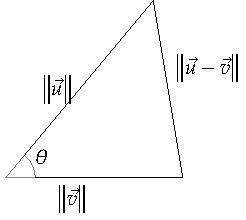
\includegraphics{lei-cossenos-vetores-plano-cartesiano.pdf}
  % \begin{tikzpicture}
  %   \coordinate (A) at (0,0);
  %   \coordinate (X) at (3,0);
  %   \coordinate (Y) at (2.5,3);

  %   \draw (A) -- (X)
  %   node[midway,below left]{$\norm{\vec{v}}$};
  %   \draw(A) -- (Y)
  %   node[midway,left]{$\norm{\vec{u}}$};
  %   \draw(X) -- (Y)
  %   node[midway,above right]{$\norm{\vec{u} - \vec{v}}$};

  %   % Mark the angle XAY
  %   \begin{scope}
  %     \path[clip] (A) -- (X) -- (Y);
  %     \fill[white, opacity=0.5, draw=black] (A) circle (5mm);
  %     \node at ($(A)+(30:7mm)$) {$\theta$};
  %   \end{scope}
  % \end{tikzpicture}
\end{figure}
temos
\begin{align}\label{equacaonorma}
  \norm{\vec{u} - \vec{v}}^2 = \norm{\vec{u}}^2 + \norm{\vec{v}}^2 - 2\norm{\vec{u}}\norm{\vec{v}}\cos\theta.
\end{align}

% Assim conhecendo as coordenadas dos vetores $\vec{u}$ e $\vec{v}$ podemos determinar facilmente o \^angulo entre eles. Al\'em disso, note que se $\vec{u}$ e $\vec{v}$ s\~ao vetores ortogonais, ent\~ao $\theta = \pi/2$ e ent\~ao a equa\c{c}\~ao \eqref{equacaonorma} torna-se
% \begin{align}\label{norma-vetores-ortogonais}
%   \norm{\vec{u} - \vec{v}} = \sqrt{\norm{\vec{u}}^2 + \norm{\vec{v}}^2}.
% \end{align}

% \begin{observacao}
%   A equa\c{c}\~ao \eqref{norma-vetores-ortogonais} s\'o \'e v\'alida para vetores ortogonais entre si.
% \end{observacao}

\begin{definicao}\label{produtointerno}
  O \textbf{produto escalar} ou \textbf{produto interno} dos vetores $\vec{u}$ e $\vec{v}$, indicado por $\inner{\vec{u}}{\vec{v}}$, \'e o n\'umero real tal que:\index{Vetores!Produto Escalar}
  \begin{enumerate}
    \item Se $\vec{u}$ ou $\vec{v}$ \'e nulo, ent\~ao $\inner{\vec{u}}{\vec{v}} = 0$.
    \item Se $\vec{u}$ e $\vec{v}$ n\~ao s\~ao nulos e $\theta$ \'e o \^angulo entre $\vec{u}$ e $\vec{v}$, ent\~ao
    \begin{align}\label{produto-interno}
      \inner{\vec{u}}{\vec{v}} = \norm{\vec{u}}\norm{\vec{v}}\cos\theta.
    \end{align}
  \end{enumerate}
\end{definicao}

\begin{proposicao}
  Sejam $\vec{u}$ e $\vec{v}$ vetores e $\theta$ o \^angulo entre $\vec{u}$ e $\vec{v}$.
  \begin{enumerate}
    \item Se $\vec{u}$ e $\vec{v}$ n\~ao s\~ao nulos, ent\~ao
    \[
      \cos\theta = \dfrac{\inner{\vec{u}}{\vec{v}}}{\norm{\vec{u}}\norm{\vec{v}}}.
    \]
    \item Qualquer que seja o vetor $\vec{u}$,
    \[
      \norm{\vec{u}} = \sqrt{\inner{\vec{u}}{\vec{u}}}.
    \]
    \item Quaisquer que sejam os vetores $\vec{u}$ e $\vec{v}$, $\vec{u}\perp\vec{v}$ se, e somente se, $\inner{\vec{u}}{\vec{v}} = 0$.
    \end{enumerate}
\end{proposicao}
\begin{prova}
  \begin{enumerate}
    \item Basta isolar $\cos\theta$ na Defini\c{c}\~ao \ref{produto-interno}.
    \item Se $\vec{u} = \vec{0}$, ent\~ao a igualdade \'e verdadeira. Se $\vec{u} \ne \vec{0}$, ent\~ao o \^angulo entre o vetor $\vec{u}$ e ele mesmo \'e $\theta = 0$, logo
    \[
      1 = \cos\theta = \dfrac{\vec{u}\cdot\vec{u}}{\norm{\vec{u}}\norm{\vec{u}}}.
    \]
    Logo
    \[
      \norm{\vec{u}} = \sqrt{\vec{u}\cdot\vec{u}}.
    \]
    \item Se $\vec{u}$ ou $\vec{v}$ \'e o vetor nulo, ent\~ao $\vec{u}\perp\vec{v}$ e $\vec{u}\cdot\vec{v} = 0$. Suponha $\vec{u} \ne \vec{0}$ e $\vec{v} \ne \vec{0}$. Assim, se $\vec{u} \perp\vec{v}$, ent\~ao $\theta = \pi/2$ e da{\'\i} $\vec{u}\cdot\vec{v} = 0$. Agora, se $\vec{u}\cdot\vec{v} = 0$, ent\~ao
    \[
      0 = \vec{u}\cdot\vec{v} = \norm{\vec{u}}\norm{\vec{v}}\cos\theta.
    \]
    Logo devemos ter $\cos\theta = 0$, isto \'e, $\theta = \pi/2$. Portanto $\vec{u}\perp\vec{v}$, como quer{\'\i}amos.
  \end{enumerate}
\end{prova}

Agora, como podemos encontrar o produto interno sem necessitar de determinar o \^angulo $\theta$ entre dois vetores $\vec{u}$ e $\vec{v}$? Substituindo o produto interno na equa\c{c}\~ao \eqref{equacaonorma} temos
\[
  \norm{\vec{u} - \vec{v}}^2 = \norm{\vec{u}}^2 + \norm{\vec{v}}^2 - 2\vec{u}\cdot\vec{v}
\]
isto \'e,
\begin{align}\label{equacao-auxilar-norma}
  \vec{u}\cdot\vec{v} = \dfrac{1}{2}(\norm{\vec{u}}^2 + \norm{\vec{v}}^2 - \norm{\vec{u} - \vec{v}}^2).
\end{align}
Se $\vec{u} = (x_1, y_1)$ e $\vec{v} = (x_2, y_2)$, ent\~ao podemos reescrever \eqref{equacao-auxilar-norma} como
\begin{align*}
  \vec{u}\cdot\vec{v} &= \dfrac{1}{2}(x_1^2 + y_1^2 + x_2^2 + y_2^2 - \norm{(x_1 - x_2, y_1 - y_2)}^2)\\
  &= \dfrac{1}{2}[x_1^2 + y_1^2 + x_2^2 + y_2^2 - (x_1 - x_2)^2 - (y_1 - y_2)^2]\\
  &= x_1x_2 + y_1y_2.
\end{align*}

Abacamos de demonstrar o seguinte teorema:
\begin{teorema}
  O produto interno de dois vetores $\vec{u} = (x_1, y_1)$ e $\vec{v} = (x_2, y_2)$ em $\real^2$ \'e dada por
  \[
    \vec{u}\cdot\vec{v} = x_1x_2 + y_1y_2.
  \]
\end{teorema}

\begin{exemplos}
  \begin{enumerate}
    \item Sejam $\vec{u} = (1, 1)$ e $\vec{v} = (1,0)$. Determine o \^angulo entre $\vec{u}$ e $\vec{v}$.
    \begin{solucao}
      Temos
      \begin{align*}
        \vec{u}\cdot\vec{v} = (1, 1)\cdot(1,0) = 2 + 0 = 1\\
        \norm{\vec{u}} = \sqrt{2},\ \norm{\vec{v}} = \sqrt{1}\\
        \cos\theta = \frac{\vec{u}\cdot\vec{v}}{\norm{\vec{u}}\norm{\vec{v}}} = \dfrac{1}{\sqrt{2}}.
      \end{align*}
      Assim, $\theta = \pi/4$.
    \end{solucao}
    \item Encontre um vetor $\vec{u} = (x, y)$ ortogonal a $\vec{v} = (4, -1)$ e tal que $\vec{u}\cdot\vec{w} = -1$, onde $\vec{w} = (1,1)$.
    \begin{solucao}
      Como $\vec{u}\cdot\vec{v} = 0$ e $\vec{u}\cdot\vec{w} = -1$ obtemos o sistema
      \[
        \begin{cases}
          4x - y = 0\\
          x + y = -1
        \end{cases}
      \]
      cuja solu\c{c}\~ao \'e $x = -1/5$ e $y = -4/5$. Logo $\vec{u} = (-1/5, -4/5)$.
    \end{solucao}
  \end{enumerate}
\end{exemplos}

\begin{proposicao}\label{propriedades-produto-interno}
  Quaisquer que sejam os vetores $\vec{u} = (x_1, y_1)$, $\vec{v} = (x_2, y_2)$ e $\vec{w} = (x_3, y_3)$ e qualquer que seja o n\'umero real $\lambda$ temos
  \begin{enumerate}[label=({\roman*})]
    \item\label{linearidade-produto-interno} $\vec{u}\cdot(\vec{v} + \vec{w}) = \vec{u}\cdot\vec{v} + \vec{u}\cdot\vec{w}$
    \item\label{linearidade2-produto-interno} $\vec{u}\cdot(\lambda\vec{v}) = \lambda(\vec{u}\cdot\vec{v})$
    \item $\vec{u}\cdot\vec{v} = \vec{v}\cdot\vec{u}$
    \item Se $\vec{u} \ne \vec{0}$, ent\~ao $\vec{u}\cdot\vec{u} > 0$.
  \end{enumerate}
\end{proposicao}
\begin{prova}
  \begin{enumerate}[label=({\roman*})]
    \item \begin{align*}
      \vec{u}\cdot(\vec{v} + \vec{w}) &= \vec{u}\cdot(x_2 + x_3, y_2 + y_3) = x_1(x_2 + x_3) + y_1(y_2 + y_3) \\ &= (x_1x_2 + y_1y_2) + (x_1x_3 + y_1y_3) = \vec{u}\cdot\vec{v} + \vec{u}\cdot\vec{w}
    \end{align*}
    \item \begin{align*}
      \vec{u}\cdot(\lambda\vec{v}) = \vec{u}\cdot(\lambda x_2, \lambda y_2) = x_1(\lambda x_2) + y_1(\lambda y_2) = (\lambda x_1)y_2 + (\lambda y_1)y_2 = (\lambda\vec{u})\cdot\vec{v}\\
      \vec{u}\cdot(\lambda\vec{v}) = \vec{u}\cdot(\lambda x_2, \lambda y_2) = x_1(\lambda x_2) + y_1(\lambda y_2) = \lambda (x_1y_2) + \lambda (y_1y_2) = \lambda(\vec{u}\cdot\vec{v})
    \end{align*}
    \item $\vec{u}\cdot\vec{v} = x_1x_2 + y_1y_2 = x_2x_1 + y_2y_1 = \vec{v}\cdot\vec{u}$
    \item Se $\vec{u} \ne \vec{0}$, ent\~ao $x_1 \ne 0$ ou $y_1 \ne 0$. Da{\'\i} $\vec{u}\cdot\vec{u} = x_1^2 + y_1^2 > 0$, como quer{\'\i}amos.
  \end{enumerate}
\end{prova}

\begin{observacao}
  \begin{enumerate}
    \item As propriedades \ref{linearidade-produto-interno} e \ref{linearidade2-produto-interno} Proposi\c{c}\~ao \ref{propriedades-produto-interno} podem ser estendidas para qualquer n\'umero de vetores e escalares:
    \[
      \vec{u}\cdot(\lambda_1\vec{v_1} + \lambda_2\vec{v_2} + \cdots + \lambda_n\vec{v_n} ) = \lambda_1\vec{u}\cdot\vec{v_1} + \lambda_2\vec{u}\cdot\vec{v_2} + \cdots + \lambda_n\vec{u}\cdot\vec{v_n}.
    \]
    \item Na igualdade $\vec{u}\cdot\vec{v} = \vec{u}\cdot\vec{w}$ n\~ao podemos concluir que $\vec{v} = \vec{w}$. Por exemplo, para $\vec{u} = (1, 0)$, $\vec{v} = (2, 1)$ e $\vec{w} = (2, -5)$ temos $\vec{u}\cdot\vec{v} = \vec{u}\cdot\vec{w}$ e no entanto $\vec{v} \ne \vec{w}$. Mas podemos concluir que $\vec{u}\perp(\vec{v} - \vec{w})$.
    \item De $\vec{u}\cdot\vec{v} = 0$ n\~ao podemos concluir que $\vec{u} = \vec{0}$ ou $\vec{v} = \vec{0}$. Por exemplo, para $\vec{u} = (2, 1)$ e $\vec{v} = (-2, 4)$ temos $\vec{u}\cdot\vec{v} = 0$ e no entanto $\vec{u} \ne \vec{0}$ e $\vec{v} \ne \vec{0}$.
  \end{enumerate}
\end{observacao}

\begin{exemplos}
  Calcule o \^angulo $\alpha$ entre $\vec{u} + \vec{v}$ e $\vec{u} - \vec{v}$, sabendo que $\norm{\vec{u}} = \sqrt{5}$, $\norm{\vec{v}} = 1$ e que o \^angulo $\theta$ entre $\vec{u}$ e $\vec{v}$ \'e $\pi/4$.
  \begin{solucao}
    Temos
    \begin{align*}
      \cos\alpha = \dfrac{(\vec{u} + \vec{v})\cdot(\vec{u} - \vec{v})}{\norm{\vec{u} + \vec{v}}\norm{\vec{u} - \vec{v}}} = \dfrac{\vec{u}\cdot\vec{u} - \vec{u}\cdot\vec{v} + \vec{v}\cdot\vec{u} - \vec{v}\cdot\vec{v}}{\norm{\vec{u} + \vec{v}}\norm{\vec{u} - \vec{v}}} = \dfrac{\norm{\vec{u}}^2 - \norm{\vec{v}}^2}{\norm{\vec{u} - \vec{v}}\norm{\vec{u} - \vec{v}}} = \dfrac{4}{\norm{\vec{u} + \vec{v}}\norm{\vec{u} - \vec{v}}}.
    \end{align*}
    Agora
    \begin{align*}
      \norm{\vec{u} + \vec{v}}^2 = (\vec{u} + \vec{v})\cdot(\vec{u} + \vec{v}) = \vec{u}\cdot\vec{u} + 2\vec{u}\cdot\vec{v} + \vec{v}\cdot\vec{v} = 6 + 2\vec{u}\cdot\vec{v}\\
      \norm{\vec{u} - \vec{v}}^2 = (\vec{u} - \vec{v})\cdot(\vec{u} - \vec{v}) = \vec{u}\cdot\vec{u} - 2\vec{u}\cdot\vec{v} + \vec{v}\cdot\vec{v} = 6 - 2\vec{u}\cdot\vec{v}.
    \end{align*}
    Por outro lado temos
    \begin{align*}
      \vec{u}\cdot\vec{v} = \norm{\vec{u}}\norm{\vec{v}}\cos\theta = \sqrt{5}\cos(\pi/4) = \dfrac{\sqrt{10}}{2}
    \end{align*}
    e ent\~ao
    \begin{align*}
      \norm{\vec{u} + \vec{v}} = \sqrt{6 + \sqrt{10}}\\
      \norm{\vec{u} - \vec{v}} = \sqrt{6 - \sqrt{10}}.
    \end{align*}
    Portanto
    \[
      \cos\theta = \dfrac{4}{\sqrt{26}}
    \]
    e ent\~ao $\theta = \arccos\left(\dfrac{4}{\sqrt{26}}\right)$.
  \end{solucao}
\end{exemplos}

\begin{proposicao}\label{DesigualdadeTriangular}
  Sejam $\vec{u}$ e $\vec{v}$ vetores.
  \begin{enumerate}
    \item $|\vec{u}\cdot\vec{v}| \le \norm{\vec{u}}\norm{\vec{v}}$ [Desigualdade de Scharwz]\index{Desigualdade de Scharwz}
    \item $\norm{\vec{u} + \vec{v}} \le \norm{\vec{u}} + \norm{\vec{v}}$ [Desigualdade Triangular]\index{Desigualdade Triangular}
  \end{enumerate}
\end{proposicao}
\begin{prova}
  \begin{enumerate}
    \item Se $\vec{u} = \vec{0}$ ou $\vec{v} = \vec{0}$ a desigualdade \'e verdadeira. Suponha ent\~ao que $\vec{u} \ne \vec{0}$ e $\vec{v} \ne \vec{0}$. Seja $\theta$ o \^angulo entre $\vec{u}$ e $\vec{v}$. Temos
    \[
      0 \le |\cos\theta| \le 1
    \]
    e multiplicando essa inequa\c{c}\~ao por $\norm{\vec{u}}\norm{\vec{v}}$ obtemos
    \[
      0 \le \norm{\vec{u}}\norm{\vec{v}}\cos\theta \le \norm{\vec{u}}\norm{\vec{v}},
    \]
    isto \'e,
    \[
      |\vec{u}\cdot\vec{v}| \le \norm{\vec{u}}\norm{\vec{v}}
    \]
    como quer{\'\i}amos.
    \item Se $\vec{u} = \vec{0}$ ou $\vec{v} = \vec{0}$, ent\~ao a desigualdade \'e verdadeira. Suponha ent\~ao que $\vec{u} \ne \vec{0}$ e $\vec{v} \ne \vec{0}$. Temos
    \begin{align*}
      \norm{\vec{u} + \vec{v}}^2 &= (\vec{u} + \vec{v})\cdot(\vec{u} + \vec{v}) = \vec{u}\cdot\vec{u} + 2\vec{u}\cdot\vec{v} + \vec{v}\cdot\vec{v} = \norm{\vec{u}}^2 + 2\vec{u}\cdot\vec{v} + \norm{\vec{v}}^2 \\ &\le \norm{\vec{u}}^2 + 2\mid\vec{u}\cdot\vec{v}\mid + \norm{\vec{v}}^2.
    \end{align*}
    Agora, usando o item (a) temos
    \begin{align*}
      \norm{\vec{u} + \vec{v}}^2 \le \norm{\vec{u}} + 2\mid\vec{u}\cdot\vec{v}\mid \norm{\vec{v}}^2 \le \norm{\vec{u}} + 2\norm{\vec{u}}\norm{\vec{v}} + \norm{\vec{v}}^2 = (\norm{\vec{u}} + \norm{\vec{v}})^2.
    \end{align*}
    Portanto
    \[
      \norm{\vec{u} + \vec{v}} \le \norm{\vec{u}} + \norm{\vec{v}}.
    \]
  \end{enumerate}
\end{prova}

% subsection angulo_entre_vetores_e_produto_interno (end)
\subsection{Proje\c{c}\~ao de Vetores} % (fold)
\label{sub:projecao_de_vetores}
Sejam $\vec{u} = (x_1, y_1)$ e $\vec{v} = (x_2, y_2)$ vetores n\~ao nulos. Suponha que o \^angulo $\theta$ entre $\vec{u}$ e $\vec{v}$ \'e tal que $0 < \theta < \pi/2$.
\begin{figure}[!h]
  \centering
  \caption{Proje\c{c}\~ao ortogonal}
  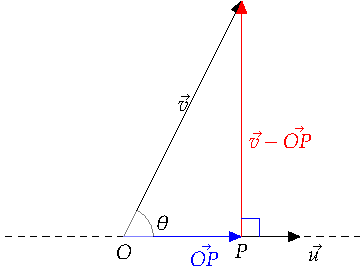
\includegraphics{projecao-vetores-plano-cartesiano.pdf}
  % \begin{tikzpicture}[scale=2]
  %   \coordinate [label=below:$O$] (O) at (0,0);
  %   \coordinate (V) at (1,2);
  %   \coordinate (U) at (1.5,0);
  %   %\coordinate (B) at (0,1);
  %   \coordinate[label=below:$P$] (P) at ($(O)!(V)!(U)$);
  %   %defini\c{c}\~ao das coordenadas dos eixos cartesianos
  %   \coordinate (F) at (-1,0);
  %   \coordinate (X) at (2,0);
  %   % Styles
  %   \tikzstyle{axes}=[]

  %   \begin{scope}[style=axes]%constr\'oi os eixos cartesianos
  %   \draw[dashed] (F) -- (X) coordinate(x axis);
  %   %\draw[->] (G) -- (Y) node[left] {$y$} coordinate(y axis);
  %   \end{scope}

  %   \draw[->,>=triangle 45] (O)--(V)
  %     node[above,midway]{$\vec{v}$};
  %   \draw[->,>=triangle 45] (O)--(U)
  %     node[below right]{$\vec{u}$};
  %   \draw[->,>=triangle 45,blue] (O)--(P)
  %     node[midway,below right]{$\vec{OP}$};
  %   \draw[->,>=triangle 45,red] ($(O)!(V)!(U)$) -- (V)
  %     node[midway,below right]{$\vec{v} - \vec{OP}$};
  %   \draw[anchor=base,color=blue] (P.center)  ++(.15,0)  -- ++(0,0.15) -- ++(-0.15,0);
    
  %   % Mark the angle XAY
  %   \begin{scope}
  %   \path[clip] (O) -- (V) -- (U);
  %   \fill[white, opacity=0.5, draw=black] (O) circle (2.5mm);
  %   \node at ($(O)+(20:3.5mm)$) {$\theta$};
  %   \end{scope}
  % \end{tikzpicture}
\end{figure}

O vetor $\vec{OP}$ \'e paralelo ao vetor $\vec{u}$ e o vetor $\vec{PA}$ \'e ortogonal ao vetor $\vec{u}$.

\begin{definicao}\label{projecao_ortogonal}
  Seja $\vec{u}$ um vetor n\~ao nulo. Dado qualquer vetor $\vec{v}$, o vetor $\vec{OP}$ \'e chamado de \textbf{proje\c{c}\~ao ortogonal} de $\vec{v}$ sobre $\vec{u}$, e \'e indicado por $\proj_{\vec{u}}\vec{v}$ se satisfaz as seguintes condi\c{c}\~oes:\index{Vetores!Proje\c{c}\~ao ortogonal}
  \begin{enumerate}
    \item $\vec{OP} \varparallel\vec{u}$
    \item $(\vec{v} - \vec{OP}) \perp \vec{u}$.
  \end{enumerate}
\end{definicao}

Podemos tamb\'em escrever
\begin{enumerate}
  \item $\proj_{\vec{u}}\vec{v} \varparallel\vec{u}$
    \item $(\vec{v} - \proj_{\vec{u}}\vec{v}) \perp \vec{u}$.
\end{enumerate}

No caso acima temos
\[
  \cos\theta = \dfrac{\norm{\vec{OP}}}{\norm{\vec{v}}}
\]
e ent\~ao $\norm{\vec{OP}} = \norm{\vec{v}}\cos\theta$. Mas
\[
  \cos\theta = \dfrac{\vec{u}\cdot\vec{v}}{\norm{\vec{u}}\norm{\vec{v}}}
\]
e assim podemos escrever
\[
  \norm{\vec{OP}} = \dfrac{\vec{u}\cdot\vec{v}}{\norm{\vec{u}}}.
\]
Al\'em disso, como $\vec{OP}$ \'e paralelo \`a $\vec{u}$ e de mesmo sentido, devemos ter $\vec{OP} = \lambda\vec{u}$ com $\lambda > 0$. Da{\'\i}
$\lambda = \norm{\vec{OP}}/\norm{\vec{u}}$ e ent\~ao
\[
  \vec{OP} = \dfrac{\norm{OP}}{\norm{\vec{u}}^2}\vec{u}.
\]

Esta constru\c{c}\~ao s\'o \'e v\'alida no caso em que o \^angulo $\theta$ entre $\vec{u}$ e $\vec{v}$ satisfaz $0 < \theta < \pi/2$. Nos casos
\begin{figure}
  \centering
  \caption{Vetor proje\c{c}\~ao}
  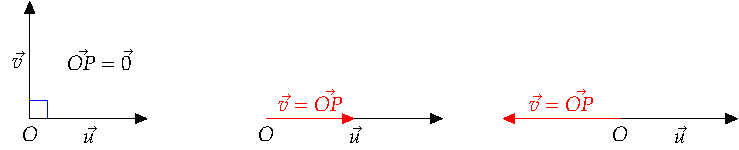
\includegraphics{vetores-projecao-plano-cartesiano.pdf}
  % \begin{tikzpicture}
  %     \coordinate[label=below:$O$] (A) at (-8,0);
  %     \coordinate (X) at (-6,0);
  %     \coordinate (Y) at (-8,2);
  %     \coordinate[label=right:$\vec{OP}\eq \vec{0}$] (P) at (-7.5,1);

  %     \draw[->,>=triangle 45] (A) -- (X)
  %     node[midway,below]{$\vec{u}$};
  %     \draw[->,>=triangle 45] (A) -- (Y)
  %     node[midway,left]{$\vec{v}$};
  %     \draw[anchor=base,color=blue] (A.center)  ++(.3,0)  -- ++(0,0.3) -- ++(-0.3,0);

  %     \coordinate[label=below:$O$] (B) at (-4,0);
  %     \coordinate (C) at (-2.5,0);
  %     \coordinate (D) at (-1,0);

  %     \draw[->,>=triangle 45] (B) -- (D)
  %     node[midway,below]{$\vec{u}$};
  %     \draw[->,>=triangle 45,red] (B) -- (C)
  %     node[midway,above]{$\vec{v} = \vec{OP}$};
      
  %     \coordinate[label=below:$O$] (B) at (2,0);
  %     \coordinate (C) at (0,0);
  %     \coordinate (D) at (4,0);

  %     \draw[->,>=triangle 45] (B) -- (D)
  %     node[midway,below]{$\vec{u}$};
  %     \draw[->,>=triangle 45,color=red] (B) -- (C)
  %     node[midway,above]{$\vec{v} = \vec{OP}$};
  %   \end{tikzpicture}
\end{figure}
n\~ao podemos usar a constru\c{c}\~ao envolvendo o \^angulo $\theta$ entre os vetores.
\begin{proposicao}
  Seja $\vec{u}$ um vetor n\~ao nulo. Qualquer que seja o vetor $\vec{v}$, existe e \'e \'unica a proje\c{c}\~ao ortogonal de $\vec{v}$ sobre $\vec{u}$. Sua express\~ao em termos de $\vec{u}$ e $\vec{v}$ \'e dada por
  \[
    \proj_{\vec{u}}\vec{v} = \dfrac{\vec{u}\cdot\vec{v}}{\norm{\vec{u}}^2}\vec{u}
  \]
  e sua norma \'e dada por
  \[
    \norm{\proj_{\vec{u}}\vec{v}} = \dfrac{\mid\vec{v}\cdot\vec{u}\mid}{\norm{\vec{u}}}.
  \]
\end{proposicao}
\begin{prova}
  Seja $\vec{p} = \proj_{\vec{u}}\vec{v}$. Da Defini\c{c}\~ao \ref{projecao_ortogonal}, dizer que $\vec{p}$ \'e a proje\c{c}\~ao ortogonal de $\vec{v}$ sobre $\vec{u}$ significa que $\vec{p}$ \'e um vetor tal que $\vec{p}\varparallel\vec{u}$ e $(\vec{v} - \vec{p})\perp\vec{u}$.

  Como $\vec{p}\varparallel\vec{u}$, ent\~ao pela Proposi\c{c}\~ao \ref{vetores_paralelos} existe um escalar $\lambda$ tal que $\vec{p} = \lambda\vec{u}$. Assim qualquer vetor do tipo $\lambda\vec{u}$ \'e um candidato para ser a proje\c{c}\~ao ortogonal. Mas, para que $\vec{p}$ seja a proje\c{c}\~ao ortogonal, ele deve satisfazer $(\vec{v} - \vec{p})\perp\vec{u}$. Logo
  \begin{align*}
    (\vec{v} - \vec{p})\perp\vec{u} \Leftrightarrow (\vec{v} - \vec{p})\cdot\vec{u} = 0 \Leftrightarrow \vec{v}\cdot\vec{u} - \lambda\vec{u}\cdot\vec{u} = 0 \Leftrightarrow \lambda = \dfrac{\vec{v}\cdot\vec{u}}{\norm{\vec{u}}^2}.
  \end{align*}
  Assim existe um \'unico $\lambda$ que satisfaz a condi\c{c}\~ao $(\vec{v} - \vec{p})\perp\vec{u}$, e da{\'\i} o vetor $\vec{p}$ \'e \'unico. Portanto
  \[
    \proj_{\vec{u}}\vec{v} = \vec{p} = \dfrac{\vec{v}\cdot\vec{u}}{\norm{\vec{u}}^2}\vec{u}.
  \]
  Al\'em disso
  \[
    \norm{\proj_{\vec{u}}\vec{v}} = \norm{\dfrac{\vec{v}\cdot\vec{u}}{\norm{\vec{u}}^2}\vec{u}} = \dfrac{\mid\vec{v}\cdot\vec{u}}{\norm{\vec{u}}}
  \]
  como quer{\'\i}amos.
\end{prova}

\begin{observacao}
  O escalar $\lambda$ encontrado na proposi\c{c}\~ao anterior pode ser negativo ou zero. Ele ser\'a negativo quando $\pi/2 \le \theta \le \pi$ e ser\'a zero quando $\vec{u}\perp\vec{v}$.
  \begin{figure}[!h]
    \centering
    \caption{Possibilidades para $\lambda$}
    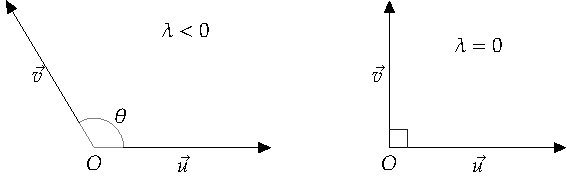
\includegraphics{vetores-projecao-escalar-plano-cartesiano.pdf}
    % \begin{tikzpicture}
    %   \coordinate[label=below:$O$] (A) at (-5,0);
    %   \coordinate (X) at (-2,0);
    %   \coordinate (Y) at (-6.5,2.5);
    %   \coordinate[label=right:$\lambda < 0$] (P) at (-4,2);

    %   \draw[->,>=triangle 45] (A) -- (X)
    %   node[midway,below]{$\vec{u}$};
    %   \draw[->,>=triangle 45] (A) -- (Y)
    %   node[midway,left]{$\vec{v}$};

    %   % Mark the angle XAY
    %   \begin{scope}
    %   \path[clip] (A) -- (X) -- (Y);
    %   \fill[white, opacity=0.5, draw=black] (A) circle (5mm);
    %   \node at ($(A)+(50:7mm)$) {$\theta$};
    %   \end{scope}
      
    %   \coordinate[label=below:$O$] (B) at (0,0);
    %   \coordinate (C) at (3,0);
    %   \coordinate (D) at (0,2.5);
    %   \coordinate[label=below:$\lambda\eq 0$] (Q) at (1.5,2);

    %   \draw[->,>=triangle 45] (B) -- (C)
    %   node[midway,below]{$\vec{u}$};
    %   \draw[->,>=triangle 45] (B) -- (D)
    %   node[midway,left]{$\vec{v}$};
    %   \draw[anchor=base,color=blue] (B.center)  ++(.3,0)  -- ++(0,0.3) -- ++(-0.3,0);

    %   % Mark the angle XAY
    %   % \begin{scope}
    %   % \path[clip] (A) -- (X) -- (Y);
    %   % \fill[white, opacity=0.5, draw=black] (A) circle (5mm);
    %   % \node at ($(A)+(30:7mm)$) {$\theta$};
    %   % \end{scope}
    %   \end{tikzpicture}
  \end{figure}
\end{observacao}

\begin{exemplos}\label{exemplosprojecao}
  \begin{enumerate}
    \item Encontre a proje\c{c}\~ao ortogonal do vetor $\vec{v} = (4, -1)$ sobre o vetor $\vec{u} = (2, 1)$.
    \begin{solucao}
       Temos
       \[
          \proj_{\vec{u}}\vec{v} = \dfrac{\vec{v}\cdot\vec{u}}{\norm{\vec{u}}^2}\vec{u}.
       \]
       Agora
       \begin{align*}
         \vec{u}\cdot\vec{v} = 7\\
         \norm{\vec{u}}^2 = 5
       \end{align*}
       e da{\'\i}
       \[
          \proj_{\vec{u}}\vec{v} = \dfrac{7}{5}(2, 1) = \left(\dfrac{14}{5}, \dfrac{7}{5}\right).
       \]
       Por outro lado,
       \[
          \proj_{\vec{v}}\vec{u} = \dfrac{\vec{u}\cdot\vec{v}}{\norm{\vec{v}}^2}\vec{v}.
       \]
       Agora
       \begin{align*}
         \vec{u}\cdot\vec{v} = \vec{v}\cdot\vec{u} = 7\\
         \norm{\vec{v}}^2 = 17
       \end{align*}
       e da{\'\i}
       \[
          \proj_{\vec{v}}\vec{u} = \dfrac{7}{17}(4, -1) = \left(\dfrac{28}{17}, \dfrac{-7}{17}\right).
       \]
     \end{solucao} 
     \item Considere um tri\^angulo $ABC$ onde $A(3,3)$, $B(0,1)$ e $C(1,6)$.
     \begin{enumerate}\label{exemploprojecao2}
       \item Verifique que $ABC$ \'e um tri\^angulo ret\^angulo em $A$.
       \item Calcule a proje\c{c}\~a do cateto $BA$ sobre a hipotenusa $BC$.
       \item Determine o p\'e da altura do tri\^angulo relativo ao v\'ertice $A$.
     \end{enumerate}
     \begin{solucao}
       Considere o tri\^angulo abaixo
       \begin{figure}[!h]
        \centering
        \caption{Exemplo \ref{exemplosprojecao}, exerc{\'\i}cio \ref{exemploprojecao2}}
        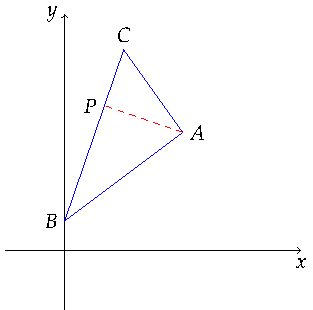
\includegraphics{exemplo-vetores-projecao-plano-cartesiano.pdf}
         % \begin{tikzpicture}[scale=2]
         %    \coordinate (o) at (0,0);
         %    \coordinate[label=right:$A$] (A) at (1,1);
         %    \coordinate[label=left:$B$] (B) at (0,0.25);
         %    \coordinate[label=above:$C$] (C) at (0.5,1.7);
         %    \coordinate[label=left:$P$] (P) at ($(C)!(A)!(B)$);
         %    %defini\c{c}\~ao das coordenadas dos eixos cartesianos
         %    \coordinate (F) at (-0.5,0);
         %    \coordinate (G) at (0,-0.5);
         %    \coordinate (X) at (2,0);
         %    \coordinate (Y) at (0,2);
         %    % Styles
         %    \tikzstyle{axes}=[]

         %    \begin{scope}[style=axes]%constr\'oi os eixos cartesianos
         %    \draw[->] (F) -- (X) node[below] {$x$} coordinate(x axis);
         %    \draw[->] (G) -- (Y) node[left] {$y$} coordinate(y axis);
         %    \end{scope}

         %    \draw[blue] (B)--(A);
         %    \draw[blue] (B)--(C);
         %    \draw[blue] (A)--(C);
         %    \draw[red,dashed] (A) -- ($(C)!(A)!(B)$);
         %  \end{tikzpicture}
       \end{figure}
       \begin{enumerate}
         \item Basta verificar que $\vec{AB}\perp\vec{AC}$. Assim como $\vec{AB} = (-3,-2)$ e $\vec{AC} = (-2,3)$ temos
         \[
            \vec{AB}\cdot\vec{AC} = (-3)(-2) + (-2)3 = 0.
         \]
         Logo $ABC$ \'e um tri\^angulo ret\^angulo.
         \item Temos $\vec{BA} = (3,2)$ e $\vec{BC} = (1,5)$. Da{\'\i}
         \[
            \proj_{\vec{BC}}\vec{BA} = \dfrac{\vec{BC}\cdot\vec{BA}}{\norm{\vec{BC}}^2}\vec{BC} = \dfrac{(3,2)\cdot(1,5)}{\norm{(1,5)}^2}(1,5) = \dfrac{13}{26}(1,5).
         \]
         Assim $\proj_{\vec{BC}}\vec{BA} = \left(\dfrac{1}{2},\dfrac{5}{2}\right)$.
         \item Seja $P(x_1, y_1)$ o p\'e da altura do tri\^angulo $ABC$ relativo ao v\'ertice $A$. Ent\~ao
         \begin{align*}
           \vec{BP} = \proj_{\vec{BC}}\vec{BA}\\
           (x_1, y_1 - 1) = \left(\dfrac{1}{2}, \dfrac{5}{2}\right).
         \end{align*}
         Logo $P\left(\dfrac{1}{2},\dfrac{7}{2}\right)$.
       \end{enumerate}
     \end{solucao}
  \end{enumerate}
\end{exemplos}
% subsection projecao_de_vetores (end)
% chapter vetores (end)
%!TEX program = xelatex
%!TEX root = geometria_analitica.tex
%%Usar makeindex -s indexstyle.ist arquivo.idx no terminal para gerar o {\'\i}ndice remissivo agrupado por inicial
%%Ap\'os executar pdflatex arquivo

\chapter{Reta no Plano} % (fold)
\label{cha:reta_no_plano}

\section{Equa\c{c}\~oes da Reta} % (fold)
\label{sec:equacoes_da_reta}

Seja $r$ uma reta do plano. Dados dois pontos $A$ e $B$ em $r$ podemos considerar o vetor $\vec{u} = \vec{AB}$. Por defini\c{c}\~ao diremos que a reta $r$ e o vetor $\vec{u}$ s\~ao paralelos. Assim temos a seguinte defini\c{c}\~ao:
\begin{definicao}
  Qualquer vetor n\~ao nulo e paralelo a uma dada reta $r$ \'e chamado de \textbf{vetor diretor} de $r$.\index{Reta no Plano!Vetor diretor}
\end{definicao}

Seja $\vec{u}$ um vetor diretor de uma reta $r$ e seja $A$ um ponto pertencente \`a reta $r$. Assim um ponto $X$ pertence a reta $r$ se, e somente se, $\vec{AX}\varparallel\vec{u}$.
\begin{figure}[!h]
  \centering
  \caption{Equa\c{c}\~ao vetorial da reta}
  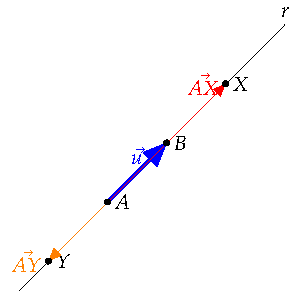
\includegraphics{equacao-vetorial-reta-plano-cartesiano.pdf}
  % \begin{tikzpicture}
  %   \coordinate[label=right:$A$] (A) at (0,0);
  %   \coordinate (U) at (-1.5,-1.5);
  %   \coordinate (V) at (3,3);
  %   \coordinate[label=right:$B$] (B) at (1,1);
  %   \coordinate[label=right:$X$] (X) at (2,2);
  %   \coordinate[label=right:$Y$] (Y) at (-1,-1);

  %   \draw (U) -- (V)
  %   node[at end,above]{$r$};

  %   \draw[ultra thick,->,>=triangle 45,blue] (A) -- (B)
  %   node[midway,above]{$\vec{u}$};
  %   \draw[->,>=triangle 45,red] (A) -- (X)
  %   node[at end,left,red]{$\vec{AX}$};
  %   \draw[->,>=triangle 45,orange] (A) -- (Y)
  %   node[at end,left,orange]{$\vec{AY}$};
  %   \foreach \p in {A,B,X,Y} \fill (\p) circle (0.5mm);
  %   \end{tikzpicture}  
\end{figure}

Ou seja, se e somente se, existe um n\'umero real $\lambda$ tal que
\begin{equation}\label{equacao_vetorial_reta_plano}
  \vec{AX} = \lambda\vec{u}.
\end{equation}

Assim para cada $\lambda \in \real$ fica definido um ponto $X$ na reta $r$ e se $X$ \'e um ponto da reta $r$, ent\~ao existe um n\'umero real $\lambda$ tal que $\vec{AX} = \lambda\vec{u}$.

\begin{definicao}\index{Reta no Plano!Equa\c{c}\~ao Vetorial}
  A equa\c{c}\~ao \eqref{equacao_vetorial_reta_plano} \'e chamada de \textbf{equa\c{c}\~ao vetorial da reta} $r$ ou \textbf{equa\c{c}\~ao da reta} $r$ \textbf{na forma vetorial}.
\end{definicao}

\begin{exemplos}
  Seja $r$ uma reta passando pelos pontos $A(1,2)$ e $B(-1, 3)$. Determine sua equa\c{c}\~ao vetorial.
  \begin{solucao}
    Um vetor diretor da reta $r$ pode ser tomado como sendo $\vec{u} = \vec{AB} = (-2, 1)$. Assim a equa\c{c}\~ao vetorial de $r$ ser\'a:
    \[
      \vec{AX} = \lambda\vec{u} = \lambda(-2,1), \quad \lambda \in \real.
    \]
    Podemos tamb\'em tomar como vetor diretor de $r$ o vetor $\vec{v} = \vec{BA} = (2,-1)$. Da{\'\i} a equa\c{c}\~ao vetorial de $r$ ser\'a
    \[
      \vec{AX} = \alpha\vec{v} = \alpha(2, -1), \quad \alpha \in \real.
    \]
  \end{solucao}
\end{exemplos}

\begin{observacao}
  Como o ponto e o vetor diretor de uma reta $r$ s\~ao escolhidos arbitrariamente, existem infinitas equa\c{c}\~oes vetorias para uma mesma reta $r$. Por exemplo, se $A$ e $B$ s\~ao pontos distintos de uma reta $r$, ent\~ao $\vec{AB}$ e $\vec{BA}$ s\~ao vetores diretores distintos de $r$ e portanto temos as equa\c{c}\~oes vetoriais
  \begin{align*}
    \vec{AX} = \lambda\vec{AB}\\
    \vec{AX} = \alpha\vec{BA}.
  \end{align*}
  Na verdade, qualquer vetor m\'ultiplo do vetor $\vec{AB}$ pode ser tomado como vetor diretor de $r$.
\end{observacao}

Agora, seja $\vec{u} = (a, b)$ um vetor diretor de uma reta $r$. Dado um ponto $A = (x_0, y_0)$ de $r$ o ponto $X = (x, y)$ pertence a reta $r$ se, e somente se, existe $\lambda \in \real$ tal que
\begin{align*}
  \vec{AX} &= \lambda\vec{u}\\
  (x - x_0, y - y_0) &= (\lambda a, \lambda b).
\end{align*}

Assim a reta $r$ pode ser descrita pelas equa\c{c}\~oes
\begin{equation}\label{equacao_parametrica_reta_plano}
  \begin{cases}
    x = x_0 + \lambda a\\
    x = y_0 + \lambda b 
  \end{cases}, \lambda \in \real
\end{equation}

\begin{definicao}\index{Reta no Plano!Equa\c{c}\~ao Param\'etrica}
  O sistema de equa\c{c}\~oes \eqref{equacao_parametrica_reta_plano} \'e chamado \textbf{sistema de equa\c{c}\~oes param\'etricas da reta} $r$ ou \textbf{sistema de equa\c{c}\~oes da reta} $r$ \textbf{na forma param\'etrica}.
\end{definicao}

\begin{exemplos}
  \begin{enumerate}
    \item O sistema de equa\c{c}\~oes
    \[
      \begin{cases}
        x = 1 + 2\lambda\\
        x = 2 - 3\lambda
      \end{cases}, \lambda \in \real
    \]
    define uma reta $r$ que passa pelo ponto $A(1,2)$ e que possui vetor diretor $\vec{u} = (2, -3)$.
    \item Seja $r$ a reta dada pelas equa\c{c}\~oes param\'etricas
    \[
      \begin{cases}
        x = 2 + 3t\\
        y = 1 + 4t
      \end{cases}, t\in \real.
    \]
    O ponto $(11, 13)$ pertence a $r$? E o ponto $(5,6)$?
    \begin{solucao}
      Para que o ponto $(11,13)$ perten\c{c}a a reta $r$ \'e preciso que exista $t \in \real$ tal que
      \begin{align*}
        11 = 2 + 3t\\
        13 = 1 + 4t.
      \end{align*}
    Cuja solu\c{c}\~ao \'e $t = 3$. Logo o ponto $(11,13)$ pertence a reta $r$.

    Para que o ponto $(5,6)$ perten\c{c}a a reta $r$ \'e preciso que exista $t \in \real$ tal que
      \begin{align*}
        5 = 2 + 3t\\
        6 = 1 + 4t.
      \end{align*}
    Resolvendo, obtemos $t = 1$ e $t = 5/4$. Logo o ponto $(5,6)$ n\~ao pertence a reta $r$.
    \end{solucao}
  \end{enumerate}
\end{exemplos}

Seja $r$ uma reta com vetor diretor $\vec{u} = (a,b)$, onde $ab\ne 0$ e que passa pelo ponto $(x_0, y_0)$. Sabemos que sua equa\c{c}\~ao param\'etrica \'e
\[
  \begin{cases}
    x = x_0 + \lambda a\\
    y = y_0 + \lambda b.
  \end{cases}
\]
Isolando $\lambda$ nas duas equa\c{c}\~oes encontramos
\[
  \lambda = \dfrac{x - x_0}{a}\quad \lambda = \dfrac{y - y_0}{b},
\]
isto \'e, a equa\c{c}\~ao
\begin{equation}\label{equacao_simetrica_reta_plano}
  \dfrac{x - x_0}{a} = \dfrac{y - y_0}{b}.
\end{equation}
determina se um ponto pertence a reta $r$ ou n\~ao.

\begin{definicao}\index{Reta no Plano!Equa\c{c}\~ao Sim\'etrica}
  A equa\c{c}\~ao \eqref{equacao_simetrica_reta_plano} \'e chamada de \textbf{sistema de equa\c{c}\~oes da reta} $r$ \textbf{na forma sim\'etrica} ou por abuso de linguagem, \textbf{equa\c{c}\~oes da reta} $r$ \textbf{na forma sim\'etrica}.
\end{definicao}

\begin{exemplos}
 Encontre a equa\c{c}\~ao sim\'etrica da reta $r$ que passa pelos pontos $A(-1,2)$ e $B(3,4)$. O ponto $(0,5/2)$ est\'a na reta $r$? E o ponto $(1,2)$?
 \begin{solucao}
   Um vetor diretor para a reta $r$ \'e dado por $\vec{u} = \vec{AB} = (4,2)$. Assim usando o ponto $A$ a equa\c{c}\~ao sim\'etrica de $r$ \'e
   \[
     \dfrac{x + 1}{4} = \dfrac{y - 2}{2}.
   \]
 Como
 \[
    \dfrac{0 + 1}{4} = \dfrac{\dfrac{5}{2} - 2}{2}
 \]
 ent\~ao o ponto $(0,5/2)$ est\'a na reta $r$. Agora como
 \[
  \dfrac{1+1}{4} \ne \dfrac{2 - 2}{2}
 \]
 o ponto $(1, 2)$ n\~ao est\'a na reta $r$.

 \end{solucao}
\end{exemplos}

\begin{observacao}
  \begin{enumerate}
    \item Para que uma equa\c{c}\~ao de uma reta $r$ esteja na forma \eqref{equacao_parametrica_reta_plano} \'e obrigat\'orio que o coeficente de $x$ e $y$ sejam 1. Assim, por exemplo a equa\c{c}\~ao na forma
    \[
      \begin{cases}
        2x = 1 - 3\lambda\\
        -y = 2 + \lambda
      \end{cases}
    \]
    n\~ao ser\'a considerada como uma equa\c{c}\~ao param\'etica de uma reta. Do mesmo modo, uma equa\c{c}\~ao do tipo
    \[
      \dfrac{2x - 7}{3} = \dfrac{y}{2}
    \]
    n\~ao ser\'a considerada uma equa\c{c}\~ao sim\'etrica de uma reta $r$ pois n\~ao est\'a na forma \eqref{equacao_simetrica_reta_plano}.

    \item Cada tipo de equa\c{c}\~ao da reta apresenta sua vantagens. A forma vetorial descreve uma reta tanto no plano cartesiano como no espa\c{c}o tridimensional e mesmo em espa\c{c}os ``maiores''. A forma param\'etrica reduz o n\'umero de inc\'ognitas com as quais precisamos trabalhar. Neste tipo de equa\c{c}\~ao lidamos com somente uma inc\'ognita em vez de duas. J\'a a forma sim\'etrica exibe qual a rela\c{c}\~ao que as coordenadas dos pontos de uma reta devem satisfazer entre si.
  \end{enumerate}
\end{observacao}

Seja $r$ uma reta que cont\'em o ponto $(x_0, y_0)$ e com vetor diretor $\vec{u} = (a, b)$. Sua equa\c{c}\~ao param\'etrica \'e
  \begin{numcases}{}
    x = x_0 + \lambda a\label{eq_parametrica1}\\
    y = y_0 + \lambda b.\label{eq_parametrica2}
  \end{numcases}

Multiplicando a equa\c{c}\~ao \eqref{eq_parametrica1} por $b$ e a equa\c{c}\~ao \eqref{eq_parametrica2} por $a$ obtemos
\begin{align}
  bx = bx_0 + \lambda ab\label{eq_parametrica_auxiliar1}\\
  ay = ay_0 + \lambda ab.\label{eq_parametrica_auxiliar2}
\end{align}

Fazendo \eqref{eq_parametrica_auxiliar2} - \eqref{eq_parametrica_auxiliar1} obtemos
\[
  ay - bx = ay_0 - bx_0.
\]

Agora note que $ay_0 - bx_0$ \'e uma constante. Assim fazendo, $c = ay_0 - bx_0$ podemos escrever
\begin{equation}\label{equacao_cartesiana_reta_plano}
  ay - bx = c
\end{equation}
que \'e chamada de \textbf{equa\c{c}\~ao cartesiana da reta} $r$.\index{Reta no Plano!Equa\c{c}\~ao Cartesiana}

Observe que se o vetor diretor $\vec{u} = (a,b)$ da reta $r$  \'e tal que $a = 0$, obtemos a equa\c{c}\~ao $x = x_0$ e a reta $r$ \'e paralela ao eixo $y$. Caso $b = 0$, obtemos $y = y_0$ e a reta \'e paralela ao eixo $x$.
\begin{figure}[!h]
  \centering
  \caption{Retas paralelas aos eixos}
  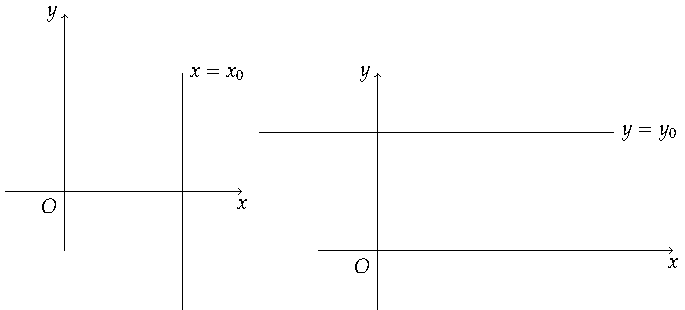
\includegraphics{retas-paralelas-plano-cartesiano.pdf}
  % \begin{tikzpicture}[scale=2]
  %   \coordinate[label=below left:$O$] (A) at (-3,0);
  %   \coordinate (W) at (-2,-1);
  %   \coordinate (V) at (-2,1);
  %   %defini\c{c}\~ao das coordenadas dos eixos cartesianos
  %   \coordinate (F) at (-3.5,0);
  %   \coordinate (G) at (-3,-0.5);
  %   \coordinate (X) at (-1.5,0);
  %   \coordinate (Y) at (-3,1.5);
  %   % Styles
  %   \tikzstyle{axes}=[]

  %   \begin{scope}[style=axes]%constr\'oi os eixos cartesianos
  %     \draw[->] (F) -- (X) node[below] {$x$} coordinate(x axis);
  %     \draw[->] (G) -- (Y) node[left] {$y$} coordinate(y axis);
  %   \end{scope}

  %   \draw  (V) -- (W)
  %     node[at start, right]{$x = x_0$};
  %   \end{tikzpicture}
  %   \begin{tikzpicture}[scale=2]
  %   \coordinate[label=below left:$O$] (A) at (0,0);
  %   \coordinate (W) at (-1,1);
  %   \coordinate (V) at (2,1);
  %   %defini\c{c}\~ao das coordenadas dos eixos cartesianos
  %   \coordinate (F) at (-0.5,0);
  %   \coordinate (G) at (0,-0.5);
  %   \coordinate (X) at (2.5,0);
  %   \coordinate (Y) at (0,1.5);
  %   % Styles
  %   \tikzstyle{axes}=[]

  %   \begin{scope}[style=axes]%constr\'oi os eixos cartesianos
  %     \draw[->] (F) -- (X) node[below] {$x$} coordinate(x axis);
  %     \draw[->] (G) -- (Y) node[left] {$y$} coordinate(y axis);
  %   \end{scope}

  %   \draw  (V) -- (W)
  %     node[at start, right]{$y = y_0$};
  %   \end{tikzpicture}
\end{figure}

Se $a \ne 0$, ent\~ao podemos dividir a equa\c{c}\~ao \eqref{equacao_cartesiana_reta_plano} por $a$ obtendo
\[
  y = \dfrac{b}{a}x + \dfrac{c}{a}.
\]
Fazendo $m = b/a$ e $k = c/a$ temos a equa\c{c}\~ao
\[
  y = mx + k,
\]
onde $m = b/a = \tan \theta$.

Note que o vetor $\vec{v} = (1,m)$ \'e paralelo \`a reta $r$ de equa\c{c}\~ao $y = mx + k$. De fato,
\begin{align*}
  \vec{v} = (1,m) = \left(1, \dfrac{b}{a}\right) = \dfrac{1}{a}(a,b) = \dfrac{1}{a}\vec{u}.
\end{align*}

\begin{exemplos}
  Determine as equa\c{c}\~oes param\'etricas e cartesianas da reta $r$ definida pelos pontos $A(1,5)$ e $B(2,7)$.
  \begin{solucao}
    Um vetor diretor de $r$ \'e dado por $\vec{u} = \vec{AB} = (1,2)$. Assim $m = b/a$ onde $\vec{u} = (a,b)$ vale $m = 2$. Desse modo temos
    \[
      y = 2x + k.
    \]
    Como o ponto $A = (1,5)$ pertence a reta $r$ devemos ter
    \[
      5 = 2(1) + k
    \]
    donde $k = 3$. Portanto a equa\c{c}\~ao cartesiana de $r$ ser\'a
    \[
      y = 2x + 3.
    \]
    A equa\c{c}\~ao param\'etrica ser\'a
    \[
      \begin{cases}
        x = 1 + \lambda\\
        y = 5 + 2\lambda
      \end{cases}, \lambda \in \real
    \]
    caso escolhamos o ponto $A$. As equa\c{c}\~oes param\'etricas de $r$ tamb\'em podem ser expressas como
    \[
      \begin{cases}
        x = 2 + \lambda\\
        y = 7 + 2\lambda
      \end{cases}, \lambda \in \real
    \]
    caso escolhamos o ponto $B$.
  \end{solucao}
\end{exemplos}
% section equacoes_da_reta (end)

\section{\^Angulo entre retas} % (fold)
\label{sec:angulo_entre_retas}
Sejam $r$ uma reta passando pelo ponto $A(x_1, y_1)$ e com vetor diretor $\vec{u} = (a,b)$ e $s$ uma reta passando pelo ponto $B(x_2, y_2)$ e com vetor diretor $\vec{v} = (c,d)$. O \textbf{\^angulo entre duas retas} $r$ e $s$ \'e definido como o menor \^angulo entre o vetor diretor $\vec{u}$ de $r$ e o vetor diretor $\vec{v}$ de $s$.

\begin{figure}[!h]
  \centering
  \caption{\^Angulo entre retas}
  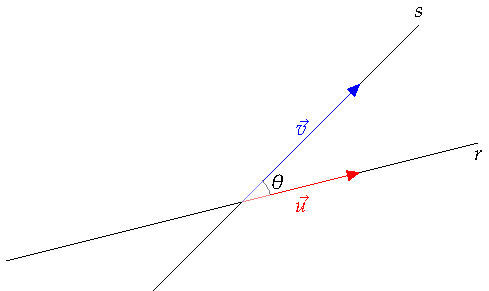
\includegraphics{angulo-retas-plano-cartesiano.pdf}
  % \begin{tikzpicture}
  %   \coordinate (A) at (0,0);
  %   \coordinate (B) at (-4,-1);
  %   \coordinate (X) at (4,1);
  %   \coordinate (C) at (-1.5,-1.5);
  %   \coordinate (Y) at (3,3);
  %   \coordinate (U) at (2,0.5);
  %   \coordinate (V) at (2,2);

  %   \draw (B) -- (X)
  %   node[at end,below]{$r$};
  %   \draw (C) -- (Y)
  %   node[at end,above]{$s$};

  %   \draw[->,>=triangle 45,red] (A) -- (U)
  %   node[midway,below]{$\vec{u}$};
  %   \draw[->,>=triangle 45,blue] (A) -- (V)
  %   node[midway,above]{$\vec{v}$};

  %   % Mark the angle XAY
  %   \begin{scope}
  %     \path[clip] (A) -- (X) -- (Y);
  %     \fill[white, opacity=0.5, draw=black] (A) circle (5mm);
  %     \node at ($(A)+(30:7mm)$) {$\theta$};
  %   \end{scope}
  % \end{tikzpicture}
\end{figure}

Assim o \^angulo $\theta$ entre $r$ e $s$ \'e dado por
\[
  \cos\theta = \dfrac{\mid\inner{u}{v}\mid}{\norm{\vec{u}}\norm{\vec{v}}},\quad 0 \le \theta \le \dfrac{\pi}{2}
\]

\begin{exemplos}
  Determine o \^angulo entre as retas $r$ e $s$ cujas equa\c{c}\~oes s\~ao:
  \begin{align*}
    r: y = 2x -2\\
    s: y = -x + 4.
  \end{align*}
  \begin{solucao}
    Temos $m = b/a$, onde $a$ e $b$ s\~ao as coordenadas do vetor diretor da reta em quest\~ao. Assim podemos tomar $\vec{u} = (1,2)$ como um vetor diretor de $r$ e $\vec{v} = (-1,1)$ como um vetor diretor de $s$. Da{\'\i}
    \[
      \cos\theta = \dfrac{\mid\inner{u}{v}\mid}{\norm{\vec{u}}\norm{\vec{v}}} = \dfrac{1}{\sqrt{10}}.
    \]
    Logo $\theta = \arccos\left(\dfrac{\sqrt{10}}{10}\right)$.
  \end{solucao}
\end{exemplos}
% section angulo_entre_retas (end)

\section{Dist\^ancia de um ponto a uma reta} % (fold)
\label{sec:distancia_de_um_ponto_a_uma_reta}
A dist\^ancia de um ponto $P(x_0,y_0)$ \`a reta $r$ de equa\c{c}\~ao $y = mx + k$ \'e definida como sendo a dist\^ancia de $P$ ao ponto $A(x_1, y_1)$, onde $A$ \'e o p\'e da perpendicular \`a reta $r$ passando pelo ponto $P$.
\begin{figure}[!h]
  \centering
  \caption{Dist\^ancia de ponto a reta}
  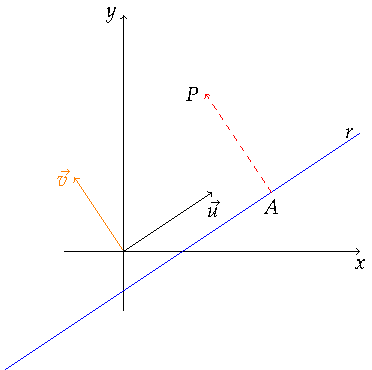
\includegraphics{distancia-ponto-reta-plano-cartesiano.pdf}
  % \begin{tikzpicture}[scale=2]%soma de vetores no plano
  %   \coordinate (D) at (-1,-1);
  %   \coordinate[label=left:$r$] (B) at (2,1);
  %   \coordinate (U) at ($0.25*(B)-0.25*(D)$);
  %   \coordinate (V) at ($(0,0)!0.75cm!90:(U)$);
  %   \draw[->,color=black] (0,0) -- (U)
  %     node[at end, below]{$\vec{u}$};
  %   \draw[->,orange] (0,0) -- (V)
  %     node[at end, left]{$\vec{v}$};
  %   \coordinate[label=below:$A$] (A) at ($(D)!.75!(B)$);
  %   \coordinate[label=left:$P$] (P) at ($(A)!1cm!90:(B)$);
  %   %defini\c{c}\~ao das coordenadas dos eixos cartesianos
  %   \coordinate (F) at (-0.5,0);
  %   \coordinate (G) at (0,-0.5);
  %   \coordinate (X) at (2,0);
  %   \coordinate (Y) at (0,2);
  %   % Styles
  %   \tikzstyle{axes}=[]

  %   \begin{scope}[style=axes]%constr\'oi os eixos cartesianos
  %     \draw[->] (F) -- (X) node[below] {$x$} coordinate(x axis);
  %     \draw[->] (G) -- (Y) node[left] {$y$} coordinate(y axis);
  %   \end{scope}

  %   \draw[blue] (D)--(B);
  %   \draw[->,red,dashed] (A) -- (P);
  % \end{tikzpicture}
\end{figure}
Agora note que o vetor $\vec{u} = (1,m)$ \'e paralelo \`a reta $r$. Al\'em disso, o vetor $\vec{v} = (-m, 1)$ \'e tal que $\inner{u}{v} = 0$, isto \'e, $\vec{u}\perp\vec{v}$. Portanto, $\vec{PA}\varparallel\vec{v}$ e ent\~ao existe $\lambda \in \real$ tal que
\[
  \vec{PA} = \lambda\vec{v}.
\]
Logo
\begin{equation}\label{distancia_ponto_reta_plano}
  d(P,r) = \norm{\vec{AP}} = \norm{\lambda\vec{v}} = \mid\lambda\mid \norm{\vec{v}} = \mid\lambda\mid\sqrt{m^2 + 1}.
\end{equation}
Assim para determinarmos $d(P,r)$ basta conhecer $\lambda$. Agora,
\[
  \vec{PA} = (x_1 - x_0, y_1 - y_0) = \lambda(-m, 1)
\]
donde
\begin{align*}
  x_1 = x_0 - \lambda m\\
  y_1 = y_0 + \lambda.
\end{align*}
Como $A(x_1, y_1)$ pertence a reta $r$, devemos ter
\begin{align*}
  y_1 = mx_1 + k\\
  y_0 + \lambda = m(x_0 - \lambda m) + k\\
  y_0 + \lambda = mx_0 - \lambda m^2 + k\\
  \lambda = \dfrac{-y_0 + mx_0 + k}{1 + m^2}.
\end{align*}
Substituindo $\lambda$ em \eqref{distancia_ponto_reta_plano}
\[
  d(P, r) = \left|\dfrac{-y_0 + mx_0 + k}{1 + m^2}\right|\sqrt{m^2 + 1}.
\]
Portanto
\[
  d(P, r) = \dfrac{\mid mx_0 + k - y_0\mid}{\sqrt{m^2 + 1}}
\]
\'e a express\~ao para a dist\^ancia de um ponto $P(x_0,y_0)$ at\'e uma reta $r$ de equa\c{c}\~ao $y = mx + k$.

\begin{exemplos}
  Seja $r$ a reta de equa\c{c}\~ao $y = 3x - 1$. Qual a dist\^ancia do ponto $P(2,2)$ \`a reta $r$?
  \begin{solucao}
    \[
      d(P,r) = \dfrac{\mid 3(2) - 1 - 2\mid}{\sqrt{3^2 + 1}} = \dfrac{3}{\sqrt{10}}.
    \]
  \end{solucao}
\end{exemplos}
% section distancia_de_um_ponto_a_uma_reta (end)



% chapter reta_no_plano (end)
%!TEX program = xelatex
%!TEX root = geometria_analitica.tex
%%Usar makeindex -s indexstyle.ist arquivo.idx no terminal para gerar o {\'\i}ndice remissivo agrupado por inicial
%%Ap\'os executar pdflatex arquivo

\chapter{Circunfer\^encias e C\^onicas} % (fold)
\label{cha:circunferencias_e_conicas}

\section{Equa\c{c}\~oes da Circunfer\^encia} % (fold)
\label{sec:equacoes_da_circunferencias}

\begin{definicao}
  A circunfer\^encia \'e o conjunto dos pontos do plano que est\~ao a uma mesma dist\^ancia (denominada \textbf{raio}) de um dado ponto do plano (chamado \textbf{centro}).\index{Circunfer\^encia}
\end{definicao}

Considere uma circunfer\^encia de centro $C(x_0,y_0)$ e raio $r$. Seja $P(x,y)$ um ponto qualquer desta circunfer\^encia e seja $\beta$ o \^angulo formado pelos vetores $\vec{CA}$ e $\vec{CP}$, onde $A(x_0 + r, y_0)$. Assim
\[
  \cos\beta = \dfrac{\inner{CA}{CPq}}{\norma{\vec{CA}}\norm{\vec{CP}}}.
\]

Mas $\vec{CP} = (x - x_0, y - y_0)$, $\vec{CA} = (r, 0)$ e $\norm{\vec{CA}} = \norm{\vec{CP}} = r$, ent\~ao
\[
  \cos\beta = \dfrac{(x - x_0)r}{r^2} = \dfrac{x - x_0}{r},
\]
isto \'e,
\begin{equation}\label{equacaoparametricaX}
  x = x_0 + r\cos\beta
\end{equation}

Agora, para os vetores $\vec{CP}$ e $\vec{CB}$, onde $B(x_0, y_0 + r)$ temos $\vec{CP} = (x - x_0, y - y_0)$, $\vec{CB} = (0, r)$ e $\norm{\vec{CA}} = \norm{\vec{CB}} = r$, ent\~ao
\begin{equation}\label{equacaoinicialY}
  \cos\alpha = \dfrac{y - y_0}{r}.
\end{equation}

\begin{figure}[h]
  \centering
  \caption{Circunfer\^encia}\label{circunferencia}
  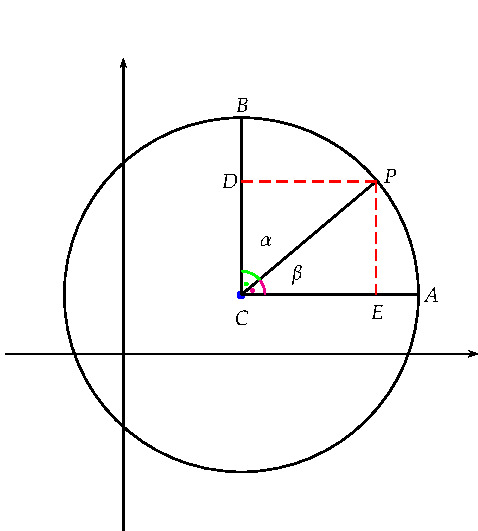
\includegraphics{circunferencia.pdf}
  % \psset{PointSymbol=none}
  % \psset{ticksize=0pt}
  % \begin{pspicture*}(-2,-3)(6,6)
  %   \psaxes[labels=none]{->}(0,0)(-1.99,-2.99)(6,5)
  %   \psdots[linecolor=blue](2,1)
  %   \pscircle(2,1){3}
  %   \pnode(2,1){A}
  %   \rput(2,0.6){$C$}
  %   \pnode(5,1){B}
  %   \rput(5.2,1){$A$}
  %   \pnode(2,4){C}
  %   \rput(2,4.2){$B$}
  %   \pnode(4.28,2.92){P}
  %   \rput(4.5,3){$P$}
  %   \rput(4.28,0.7){$E$}
  %   \rput(1.8,2.92){$D$}
  %   \psline(2,1)(5,1)
  %   \psline(2,1)(2,4)
  %   \psline(2,1)(4.28,2.92)
  %   \psline[linestyle=dashed,linecolor=red](4.28,1)(4.28,2.92)
  %   \psline[linestyle=dashed,linecolor=red](2,2.92)(4.28,2.92)
  %   \pstRightAngle[linecolor=magenta, RightAngleType=german]{B}{A}{P}
  %   \pstMarkAngle[linecolor=magenta]{B}{A}{P}{$\beta$}
  %   \pstRightAngle[linecolor=green, RightAngleType=german]{P}{A}{C}
  %   \pstMarkAngle[linecolor=green]{P}{A}{C}{$\alpha$}
  % \end{pspicture*}
\end{figure}

Na Figura \ref{circunferencia}, considere o p\'e da perpendicular ao segmento $CA$ passando por $P$ e denote esse ponto por $E$. Agora, considere o p\'e da perpendicular ao segmento $CB$ passando por $P$ e denote esse ponto por $D$. Ent\~ao os segmentos $CD$ e $EP$ t\^em o mesmo comprimento $k$. Da{\'\i}
\begin{equation}\label{equacaosenocosseno}
  \cos\alpha = \dfrac{k}{r} = \sin\beta.
\end{equation}

Substituindo \eqref{equacaosenocosseno} em \eqref{equacaoinicialY} obtemos:
\[
  \sin\beta = \dfrac{y - y_0}{r},
\]
isto \'e,
\begin{equation}\label{equacaoparametricaY}
   y = y_0 + r\sin\beta.
\end{equation}

Por outro lado, se um ponto $P(x, y)$ satisfaz as equa\c{c}\~oes \eqref{equacaoparametricaX} e \eqref{equacaoparametricaY}, ent\~ao
\[
  d(P,C) = \sqrt{(x - x_0)^2 + (y - y_0)^2} = \sqrt{r^2\cos^2\beta + r^2\sin^2\beta} = r
\]
e ent\~ao o ponto $P$ pertence \`a circunfer\^encia de centro $C(x_0,y_0)$ e raio $r$.

\begin{definicao}
  As equa\c{c}\~oes
  \[
    \begin{cases}
      x = x_0 + r\cos\beta\\
      y = y_0 + r\sin\beta,
    \end{cases}
    \beta \in [0,2\pi]
  \]
  s\~ao chamadas \textbf{equa\c{c}\~oes param\'etricas} da circunfer\^encia de centro $C(x_0, y_0)$ e raio $r$.\index{Circunfer\^encia!Equa\c{c}\~oes Param\'etricas}
\end{definicao}

Seja $C$ uma circunfer\^encia com equa\c{c}\~oes param\'etricas
\[
    \begin{cases}
      x = x_0 + r\cos\beta\\
      y = y_0 + r\sin\beta,
    \end{cases}
    \beta \in [0,2\pi].
\]

Podemos escrever
\begin{align*}
  x - x_0 = r\cos\beta\\
  y - y_0 = r\sin\beta.
\end{align*}
Elevando ao quadrado ambos os lados
\begin{align*}
  (x - x_0)^2 = r^2\cos^2\beta\\
  (y - y_0)^2 = r^2\sin^2\beta
\end{align*}
e somando obtemos
\begin{equation}
  (x - x_0)^2 + (y - y_0)^2 = r^2
\end{equation}
que \'e a \textbf{equa\c{c}\~ao cartesiana} da circunfer\^encia de centro $(x_0,y_0)$ e raio $r$.\index{Circunfer\^encia!Equa\c{c}\~ao Cartesiana}
Podemos reescrever essa equa\c{c}\~ao como
\[
  x^2 + y^2 - 2x_0x - 2y_0y + x_0^2 + y_0^2 - r^2 = 0.
\]
Fazendo
\[
  -2x_0 = a,\quad -2y_0 = b,\quad x_0^2 + y_0^2 - r^2 = c
\]
obtemos
\begin{equation}\label{equacaoalternativacircunferencia}
  x^2 + y^2 + ax + by + c = 0.
\end{equation}

Sejam $P_1(x_1,y_1)$, $P_2(x_2,y_2)$ e $P_3(x_3,y_3)$ tr\^es pontos n\~ao colineares, isto \'e, os vetores $\vec{P_1P_2}$ e $\vec{P_1P_3}$ n\~ao s\~ao paralelos. Nessa situa\c{c}\~ao \'e poss{\'\i}vel obter uma circunfer\^encia contendo estes tr\^es pontos. Para isso considere a equa\c{c}\~ao \eqref{equacaoalternativacircunferencia}. Para que $P_1$, $P_2$ e $P_3$ perten\c{c}am a uma circunfer\^encia $C$ devemos ter:
\begin{align*}
  x_1^2 + y_1^2 + ax_1 + by_1 + c = 0\\
  x_2^2 + y_2^2 + ax_2 + by_2 + c = 0\\
  x_3^2 + y_3^2 + ax_3 + by_3 + c = 0.
\end{align*}
Da{\'\i} para encontrar a circunfer\^encia desejada, basta determinar os valores de $a$, $b$ e $c$. Ou seja, precisamos resolver o sistema
\[
  \begin{cases}
    ax_1 + by_1 + c = -(x_1^2 + y_1^2)\\
    ax_2 + by_2 + c = -(x_2^2 + y_2^2)\\
    ax_3 + by_3 + c = -(x_3^2 + y_3^2).
  \end{cases}
\]

Como os ponto $P_1$, $P_2$ e $P_3$ n\~ao s\~ao colineares, este sistema sempre possui solu\c{c}\~ao \'unica.

\begin{exemplos}
  \begin{enumerate}
    \item Escreva a equa\c{c}\~ao cartesiana da circunfer\^encia passando pelos pontos $A(1,1)$, $B(1,-2)$ e $C(2,3)$.
    \begin{solucao}
      Temos
      \begin{align*}
        \vec{AB} = (0,-3)\\
        \vec{AC} = (1,2)
      \end{align*}
      assim os pontos n\~ao s\~ao colineares e portanto definem uma circunfer\^encia. Para encontr\'a-la, devemos resolver o sistema
      \[
        \begin{cases}
          a + b + c = -2\\
          a - 2b + c = -5\\
          2a + 3b + c = -13
        \end{cases}
      \]
      cuja solu\c{c}\~ao \'e
      \[
        a = -13,\quad b = 1 \quad\mbox{e}\quad c = 10.
      \]
      Logo
      \[
        x^2 + y^2 - 13x + y - 10 = 0
      \]
      \'e a equa\c{c}\~ao procurada.

      Agora, como
      \[
        -2x_0 = a,\quad -2y_0 = b,\quad x_0^2 + y_0^2 - r^2 = c
      \]
      segue que
      \[
        x_0 = 13/2,\quad y_0 = -1/2 \quad\mbox{e}\quad r^2 = 65/2.
      \]
      Assim a equa\c{c}\~ao cartesiana da circunfer\^encia ser\'a
    \[
      \left(x - \dfrac{13}{2}\right)^2 + \left(y + \dfrac{1}{2}\right)^2 = \dfrac{65}{2}.
    \]
    As equa\c{c}\~oes param\'etricas s\~ao
    \[
      \begin{cases}
        x = \dfrac{13}{2} + \dfrac{\sqrt{65}}{\sqrt{2}}\cos\beta\\
        y = -\dfrac{1}{2} + \dfrac{\sqrt{65}}{\sqrt{2}}\sin\beta\\
      \end{cases}, \beta \in [0,2\pi].
    \]
    \end{solucao}
    \item Encontre a equa\c{c}\~ao da circunfer\^encia que passa pelos pontos $P_1(1,-1)$, $P_2(0,1)$ e $P_3(1,0)$.
    \begin{solucao}
      Primeiro note que
      \begin{align*}
        \vec{P_1P_2} = (-1,2)\\
        \vec{P_1P_3} = (0,1).
      \end{align*}
      Assim os pontos n\~ao s\~ao colineares, portanto tal circunfer\^encia existe. Para encontr\'a-la, basta resolver o sistema
      \[
        \begin{cases}
          a - b + c = -2\\
          b + c = -1\\
          a + c = -2.
        \end{cases}
      \]
      A solu\c{c}\~ao \'e $a = b = 1$ e $c = -2$. Logo a circunfer\^encia tem equa\c{c}\~ao
      \[
        x^2 + y^2 + x + y - 2 = 0.
      \]
    \end{solucao}
    \item Encontre a equa\c{c}\~ao da circunfer\^encia que passa pelos pontos $P_1(1,3)$, $P_2(3,-5)$ e $P_3(2,-1)$.
    \begin{solucao}
      Note que
      \begin{align*}
        \vec{P_1P_2} = (2, -8)\\
        \vec{P_1P_3} = (1, -4).
      \end{align*}
      Assim $P_1$, $P_2$ e $P_3$ s\~ao colineares e portanto os tr\^es pontos n\~ao definem uma circunfer\^encia.
    \end{solucao}
  \end{enumerate}
\end{exemplos}

% section equacoes_da_circunferencias (end)

\section{C\^onicas} % (fold)
\label{sec:conicas}

\begin{definicao}
  Chama-se \textbf{c\^onica} o lugar geom\'etrico dos pontos $P(x,y)$ que satisfazem uma equa\c{c}\~ao do segundo grau $g(x,y) = 0$, onde\index{C\^onicas}
  \begin{equation}\label{equacaoconica}
    g(x,y) = ax^2 + bxy + cy^2 + dx + ey + f.
  \end{equation}
\end{definicao}

Na equa\c{c}\~ao \eqref{equacaoconica} pelo menos um dos n\'umeros $a$, $b$ $c$ \'e diferente de zero. Os termos $ax^2$ e $cy^2$ s\~ao os \textbf{termos quadr\'aticos}, o termo $bxy$ \'e o \textbf{termo quadr\'atico misto}, $dx$ e $ey$ s\~ao os \textbf{termos lineares} e $f$ \'e o \textbf{termo independente}. \index{C\^onica!Termos Quadr\'aticos} \index{C\^onica!Termo Quadr\'atico Misto} \index{C\^onica!Termos Lineares} \index{C\^onica!Termos Independete}

A equa\c{c}\~ao \eqref{equacaoconica} pode representar:
\begin{enumerate}[label=({\arabic*})]
  \item um conjunto vazio: $x^2 + y^2 = -1$;
  \item um conjunto formado por um ponto: $x^2 + y^2 = 0$;
  %\item uma reta;
  \item a reuni\~ao de duas retas (paralelas ou concorrentes): $x^2 - y^2 - 2x - 6y -8 =0$;
  \item uma circunfer\^encia: $x^2 + y^2 - 13x + y - 10 = 0$;
  \item uma elipse: $4x^2 + 9y^2 - 8x - 36y + 4 = 0$;
  \item uma hip\'erbole: $3x^2 + 3y^2 - 10xy + 12\sqrt{2}x - 4\sqrt{2}y + 32 = 0$;
  \item uma par\'abola: $x^2 - 2xy + y^2 -2x - 2y + 1 = 0$.
\end{enumerate}

Nos casos em que a equa\c{c}\~ao \eqref{equacaoconica} representar um conjunto vazio, um ponto, retas ou circunfer\^encias diremos que a c\^onica definida \'e uma \textbf{c\^onica degenerada}. Aqui vamos estudar as c\^onicas chamadas de elipse, hip\'erbole e par\'abola.

\subsection{Elipse} % (fold)
\label{sub:elipse}

\begin{definicao}
  Sejam $F_1$ e $F_2$ pontos distintos do plano, $2c$ a dist\^ancia entre $F_1$ e $F_2$ e $a$ um n\'umero real tal que $a > c$. O lugar geom\'etrico $\mathcal{E}$ dos pontos $P$ tais que
  \begin{equation}\label{definicaoelipse}
    d(P,F_1) + d(P,F_2) = 2a
  \end{equation}
  chama-se \textbf{elipse}. Cada um dos pontos $F_1$ e $F_2$ \'e chamado \textbf{foco} da elipse. O segmento $F_1F_2$ \'e chamado \textbf{segmento focal}, seu ponto m\'edio \'e o \textbf{centro} da elipse e $2c$ \'e chamado \textbf{dist\^ancia focal}. A reta passando por $F_1$ e $F_2$ chama-se \textbf{reta focal}.\index{Elipse} \index{Elipse!Focos} \index{Elipse!Centro} \index{Elipse!Reta Focal}
\end{definicao}

Para obter a equa\c{c}\~ao que descreve uma elipse vamos fixar os focos $F_1$ e $F_2$ como sendo $F_1(-c,0)$ e $F_2(c,0)$. Assim o centro dessa elipse estar\'a na origem do plano cartesiano. Assim, seja $P(x,y)$ um ponto pertencente \`a elipse de focos $F_1$ e $F_2$. Ent\~ao
\begin{equation}
  d(P,F_1) + d(P,F_2) = 2a,
\end{equation}
isto \'e,
\begin{equation}
  d(P,F_1) = 2a -  d(P,F_2).
\end{equation}
Assim,
\[
  \sqrt{(x + c)^2 + y^2} = 2a - \sqrt{(x - c)^2 + y^2}
\]
e elevando ao quadrado ambos os membros dessa igualdade obtemos
\[
  a\sqrt{(x - c)^2 + y^2} = a^2 - cx.
\]
Elevando novamente ao quadrado e simplificando
\[
  (a^2 - c^2)x^2 + a^2y^2 = a^2(a^2 - c^2).
\]
Fazendo $b^2 = a^2 - c^2$, podemos escrever
\[
  b^2x^2 + a^2y^2 = a^2b^2.
\]
Finalmente, dividindo por $a^2b^2$ obtemos
\begin{equation}\label{equacaoelipse}
  \elipse{a^2}{b^2}.
\end{equation}

Observe que
\begin{align}
  a^2 = b^2 + c^2\\
  a > b > 0\\
  a > c > 0.
\end{align}

Assim todo ponto pertencente a elipse de focos $F_1(-c,0)$ e $F_2(c,0)$, deve satisfazer a equa\c{c}\~ao
\[
  \elipse{a^2}{b^2}.
\]

Por outro lado, seja $Q(\alpha,\beta)$ um ponto tal que
\[
  \dfrac{\alpha^2}{a^2} + \dfrac{\beta^2}{b^2} = 1.
\]
Ent\~ao $\beta^2 = b^2 - (b^2/a^2)\alpha^2$ e da{\'\i}
\begin{align*}
  d^2(Q,F_1) &= (\alpha + c)^2 + \beta^2\\
&= \alpha^2 + 2c\alpha + c^2 + b^2 - \dfrac{b^2}{a^2}\alpha^2\\
&= \left(\dfrac{c}{a}\alpha + a\right)^2.
\end{align*}

Analogamente,
\begin{equation*}
  d^2(Q,F_2) = \left(\dfrac{c}{a}\alpha - a\right)^2.
\end{equation*}
Assim
\begin{align}
  d(Q,F_1) &= \left|\dfrac{c}{a}\alpha + a\right|\label{distanciaP1}\\
  d(Q,F_2) &= \left|\dfrac{c}{a}\alpha - a\right|\label{distanciaP2}.
\end{align}

Como
\[
  \dfrac{\alpha^2}{a^2} + \dfrac{\beta^2}{b^2} = 1.
\]
ent\~ao $\alpha^2/a^2 \le 1$, isto \'e, $\mid\alpha\mid\le a$. Mas $c/a > 0$, da{\'\i}
\[
  \dfrac{c}{a}\mid\alpha\mid \le c < a
\]
logo
\[
  -a < \dfrac{c\alpha}{a} < a.
\]
Portanto,
\begin{align*}
  \dfrac{c}{a}\alpha + a > 0\\
  \dfrac{c}{a}\alpha - a < 0.
\end{align*}
Desse modo podemos escrever \eqref{distanciaP1} e \eqref{distanciaP2} como
\begin{align*}
  d^2(Q,F_1) &= \dfrac{c}{a}\alpha + a\\
  d^2(Q,F_2) &= a - \dfrac{c}{a}\alpha.
\end{align*}

Assim
\[
  d(Q,F_1) + d(Q,F_2) = 2a
\]
e ent\~ao o ponto $Q(\alpha,\beta)$ pertence \`a elipse de focos $F_1(-c,0)$ e $F_2(c,0)$.

Os n\'umeros $a$, $b$ e $c$ s\~ao chamados \textbf{par\^ametros geom\'etricos} da elipse. A equa\c{c}\~ao \eqref{equacaoelipse} \'e chamada de \textbf{equa\c{c}\~ao reduzida da elipse} de centro $O(0,0)$ e focos no eixo $x$. Indicamos tal elipse por\index{Elipse!Par\^ametros Geom\'etricos} \index{Elipse!Equa\c{c}\~ao Reduzida}
\[
  \mathcal{E}: \elipse{a^2}{b^2}.
\]

Com isso provamos a seguinte proposi\c{c}\~ao:
\begin{proposicao}
  Um ponto $P(x,y)$ \'e um ponto da elipse de equa\c{c}\~ao reduzida
  \[
    \elipse{a^2}{b^2}
  \]
  se, e somente se, as dist\^ancias de $P$ aos focos $F_1$ e $F_2$ s\~ao
  \begin{align*}
    d^2(P,F_1) &= \dfrac{c}{a}\alpha + a\\
    d^2(P,F_2) &= a - \dfrac{c}{a}\alpha.
  \end{align*}
\end{proposicao}

\begin{observacao}
  \begin{enumerate}
    \item A equa\c{c}\~ao \eqref{equacaoelipse} s\'o \'e v\'alida para elipses com focos no eixo $x$ e centro na origem. Mudan\c{c}as nos focos ou no centro, resultar\~ao em uma equa\c{c}\~ao diferente para a elipse.
    \item Se $(x,y)$ satisfaz a equa\c{c}\~ao \eqref{equacaoelipse}, ent\~ao $(-x,-y)$, $(-x,y)$ e $(x,-y)$ tamb\'em satisfazem a mesma equa\c{c}\~ao. Assim a elipse \'e sim\'etrica em rela\c{c}\~ao ao eixo $x$, ao eixo $y$ e ao centro do plano cartesiano.
    \item O ponto $(x,0)$ pertence \`a elipse de equa\c{c}\~ao \eqref{equacaoelipse} se, e somente se, $x^2/a^2 = 1$, isto \'e, $x = \pm a$. Al\'em disso, o ponto $(0,y)$ pertence \'a elipse de equa\c{c}\~ao \eqref{equacaoelipse} se, e s\'o se, $y = \pm b$. Portanto, a interse\c{c}\~ao de $E$ com o eixo $x$ s\~ao os pontos $A_1(-a,0)$ e $A_2(a,0)$ e a interse\c{c}\~ao com o eixo $y$ s\~ao os pontos $B_1(0,-b)$ e $B_2(0,b)$. Note que $d(B_j,F_i) = \sqrt{c^2 + b^2} = a$, para $i$, $j = 1$, 2.
    \item N\~ao existe circunfer\^encia que contenha os pontos $A_1$, $A_2$, $B_1$ e $B_2$. Caso existisse, tal circunfer\^encia teria dois di\^ametros diferentes, cujos comprimento s\~ao dados pelos comprimentos dos segmente $A_1A_2$ e $B_1B_2$, o que \'e imposs{\'\i}vel. Portanto, como esses pontos pertencem a $E$, podemos afirmar que a elipse n\~ao \'e uma circunfer\^encia e nem o conjunto vazio.
  \end{enumerate}
\end{observacao}

Na equa\c{c}\~ao \eqref{equacaoelipse}, fazendo $y \ge 0$ podemos escrever
\[
  y = \dfrac{b}{a}\sqrt{a^2 - x^2},\quad x \in [0,a].
\]
Tal equa\c{c}\~ao \'e uma fun\c{c}\~ao em $x$, cont{\'\i}nua, decrescente e com concavidade para baixo em todo seu dom{\'\i}nio. Assim seu gr\'afico \'e dado pela Figura \ref{GraficoprimeiroquadranteElipse}.
\begin{figure}[h]
  \centering
  \caption{Gr\'afico da fun\c{c}\~ao $y = \dfrac{b}{a}\sqrt{a^2 - x^2}$}
  \label{GraficoprimeiroquadranteElipse}
  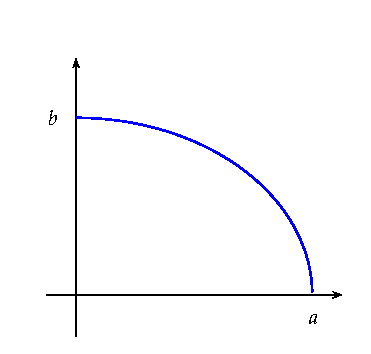
\includegraphics{grafico-elipse-primeiro-quadrante.pdf}
  % \psset{ticksize=0pt}
  % \begin{pspicture*}(-1.2,-1)(5,5)
  %   \psaxes[labels=none]{->}(0,0)(-0.5,-0.7)(4.5,4)
  %   \psplot[algebraic,linecolor=blue,plotpoints=20000]{0}{3.998888999}{(3/4)*sqrt(16 - x^2)}
  %   \rput(-0.4,3){$b$}
  %   \rput(4,-0.4){$a$}
  % \end{pspicture*}
\end{figure}

E como a elipse \'e sim\'etrica, sua forma \'e dada pela Figura \ref{FormageralElipse}.
\begin{figure}[h]
  \centering
  \caption{Elipse com focos no eixo $x$ e centro na origem: $\elipse{a^2}{b^2}$}
  \label{FormageralElipse}
  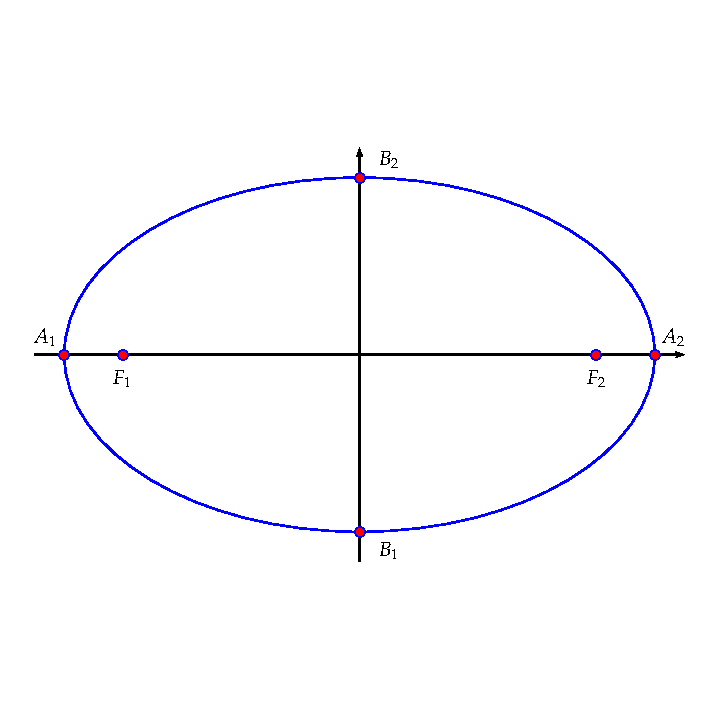
\includegraphics{elipse-focos-eixo-X.pdf}
  % \psset{ticksize=0pt}
  % \begin{pspicture*}(-7,-7)(7,7)
  %   \psaxes[labels=none]{->}(0,0)(-5.5,-3.5)(5.5,3.5)
  %   \psellipse[linecolor=blue](0,0)(5,3)
  %   \rput(5.3,0.3){$A_2$}
  %   \psdot[linecolor=blue,fillcolor=red,dotstyle=o,dotsize=5pt](5,0)
  %   \rput(-5.3,0.3){$A_1$}
  %   \psdot[linecolor=blue,fillcolor=red,dotstyle=o,dotsize=5pt](-5,0)
  %   \rput(0.5,-3.3){$B_1$}
  %   \psdot[linecolor=blue,fillcolor=red,dotstyle=o,dotsize=5pt](0,-3)
  %   \rput(0.5,3.3){$B_2$}
  %   \psdot[linecolor=blue,fillcolor=red,dotstyle=o,dotsize=5pt](0,3)
  %   \rput(4,-0.4){$F_2$}
  %   \psdot[linecolor=blue,fillcolor=red,dotstyle=o,dotsize=5pt](4,0)
  %   \rput(-4,-0.4){$F_1$}
  %   \psdot[linecolor=blue,fillcolor=red,dotstyle=o,dotsize=5pt](-4,0)
  % \end{pspicture*}
\end{figure}

\begin{definicao}
  Os pontos $A_1$ e $A_2$ em que a reta focal intercepta a elipse e os pontos $B_1$ e $B_2$ em que a mediatriz do segmento focal intercepta a elipse s\~ao chamados de \textbf{v\'ertices}. Os segmentos $A_1A_2$ e $B_1B_2$ s\~ao chamados de \textbf{eixo maior} e \textbf{eixo menor} da elipse, respectivamente.\index{Elipse!V\'ertice} \index{Elipse!Eixo Maior} \index{Elipse!Eixo Menor}
\end{definicao}

\begin{exemplos}
  \begin{enumerate}
    \item A equa\c{c}\~ao
    \[
      \elipse{9}{4}
    \]
    representa uma elipse onde $a = 3$, $b = 2$. Os focos s\~ao $F_1(-c,0)$ e $F_2(c,0)$ onde, $a^2 = b^2 + c^2$. Da{\'\i}, $c = \sqrt{5}$. Logo $F_1(-\sqrt{5},0)$ e $F_2(\sqrt{5},0)$. Os v\'ertices s\~ao $A_1(-3,0)$, $A_2(3,0)$, $B_1(0,-2)$ e $B_2(0,2)$.
    \item Encontre a equa\c{c}\~ao da elipse cujos focos s\~ao $F_1(-3,0)$ e $F_2(0,4)$ e cujo eixo maior mede 7.
    \begin{solucao}
      Como os focos n\~ao est\~ao sobre o eixo $x$, n\~ao podemos usar a equa\c{c}\~ao \eqref{equacaoelipse}. Assim vamos utilizar a defini\c{c}\~ao \eqref{definicaoelipse}. Seja $P(x,y)$ um ponto pertencente a tal elipse, ent\~ao
      \[
        d(P,F_1) + d(P,F_2) = 7.
      \]
      Assim
      \begin{align*}
        &\sqrt{(x + 3)^2 + y^2} + \sqrt{x^2 + (y - 4)^2} = 7\\
        &(x+ 3)^2 + y^2 = 49 - 14\sqrt{x^2 + (y - 4)^2} + x^2 + (y - 4)^2\\
        &(3x + 4y - 28)^2 = \left[-7\sqrt{x^2 + (y - 4)^2}\right]^2\\
        &9x^2 + 24xy + 16y^2 - 168x - 224y + 784 = 49x^2 + 49y^2 - 392y + 784
      \end{align*}
      Portanto a elipse procurada tem equa\c{c}\~ao
      \[
        40x^2 + 33y^2 - 24xy + 168x - 168y = 0.
      \]
    \end{solucao}
    \item Encontre a equa\c{c}\~ao da elipse com focos $F_1(0,-2)$ e $F_2(0,2)$ e tal que $a = 3$.
    \begin{solucao}
      Neste caso, $P(x,y)$ pertence \`a elipse se, e somente se,
      \begin{align*}
        &d(P,F_1) + d(P,F_2) = 6\\
        &\sqrt{x^2 + (y + 2)^2} + \sqrt{x^2 + (y - 2)^2} = 6\\
        &(8y - 36)^2 = \left[-12\sqrt{x^2 + (y - 2)^2}\right]^2\\
        &64y^2 - 576y + 1296 = 144x^2 + 144y^2 - 576y + 576\\
        &144x^2 + 80y^2 = 720.
      \end{align*}
      Portanto a elipse procurada tem equa\c{c}\~ao
      \[
        \elipse{5}{9}.
      \]
    \end{solucao}
  \end{enumerate}
\end{exemplos}

\begin{proposicao}
  Uma equa\c{c}\~ao da forma
  \begin{equation}\label{equacaoelipsequasegeral}
    \elipse{p}{q}
  \end{equation}
  descreve uma elipse se, e somente se, os n\'umeros reais $p$ e $q$ s\~ao distintos e positivos.
\end{proposicao}

\begin{corolario}
  Sejam $O$ a origem do plano cartesiano, $p$ e $q$ n\'umeros reais distintos e positivos. Seja $E$ a elipse de equa\c{c}\~ao \eqref{equacaoelipsequasegeral} e par\^ametros geom\'etricos $a$ e $b$.
  \begin{enumerate}
    \item Se $p > q$, ent\~ao $a^2 = p$, $b^2 = q$ e $E$ tem centro $O$ e focos no eixo $x$.
    \item Se $q > p$, ent\~ao $a^2 = q$, $b^2 = p$ e $E$ tem centro $O$ e focos no eixo $y$.
  \end{enumerate}
\end{corolario}

\begin{figure}[h]
  \centering
  \caption{Elipse com focos no eixo $y$ e centro na origem: $\elipse{a^2}{b^2}$}
  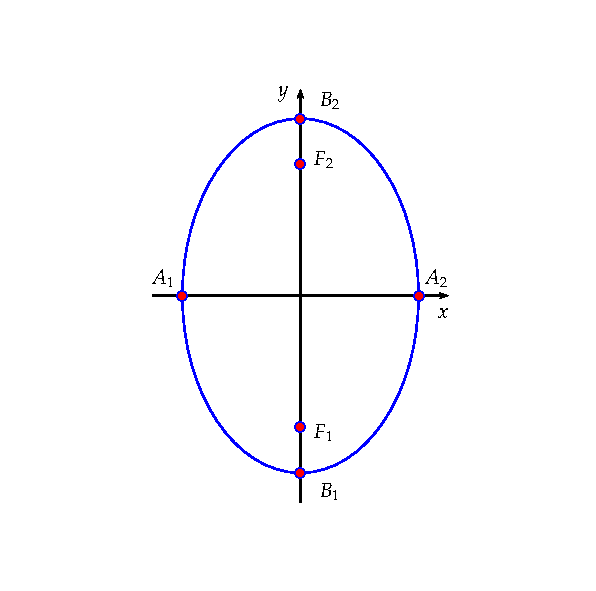
\includegraphics{elipse-focos-eixo-Y.pdf}
  % \psset{ticksize=0pt}
  % \begin{pspicture*}(-7,-7)(7,7)
  %   \psaxes[labels=none]{->}(0,0)(-2.5,-3.5)(2.5,3.5)
  %   \psellipse[linecolor=blue](0,0)(2,3)
  %   \rput(2.3,0.3){$A_2$}
  %   \psdot[linecolor=blue,fillcolor=red,dotstyle=o,dotsize=5pt](2,0)
  %   \rput(-2.3,0.3){$A_1$}
  %   \psdot[linecolor=blue,fillcolor=red,dotstyle=o,dotsize=5pt](-2,0)
  %   \rput(0.5,-3.3){$B_1$}
  %   \psdot[linecolor=blue,fillcolor=red,dotstyle=o,dotsize=5pt](0,-3)
  %   \rput(0.5,3.3){$B_2$}
  %   \psdot[linecolor=blue,fillcolor=red,dotstyle=o,dotsize=5pt](0,3)
  %   \rput(0.4,2.3){$F_2$}
  %   \psdot[linecolor=blue,fillcolor=red,dotstyle=o,dotsize=5pt](0,2.23)
  %   \rput(0.4,-2.3){$F_1$}
  %   \psdot[linecolor=blue,fillcolor=red,dotstyle=o,dotsize=5pt](0,-2.23)
  %   \rput(2.4,-0.3){$x$}
  %   \rput(-0.3,3.4){$y$}
  % \end{pspicture*}
\end{figure}


\begin{exemplos}
  Para as equa\c{c}\~oes dadas, encontre os focos, v\'ertices e o comprimento do eixo maior e menor da elipse dada.
  \begin{enumerate}
    \item $16x^2 + y^2 = 1$
    \begin{solucao}
      Podemos escrever essa equa\c{c}\~ao como
      \[
        \elipse{\dfrac{1}{16}}{1}
      \]
      e da{\'\i} $p = 1/16$ e $q = 1$. Como $p < q$, os focos est\~ao no eixo $y$. Assim $a = 1$ e $b = 1/4$. Como $a^2 = b^2 + c^2$, temos $c = \sqrt{15}/4$. Logos
      \begin{align*}
        F_1\left(0,-\dfrac{\sqrt{15}}{4}\right),\quad F_2\left(0,\dfrac{\sqrt{15}}{4}\right)\\
        A_1(0,-1),\quad A_2(0,1)\\
        B_1\left(-\dfrac{1}{4},0\right),\quad B_1\left(\dfrac{1}{4},0\right).
      \end{align*}
    \end{solucao}
    \item $25x^2 + 169y^2 = 9$
    \begin{solucao}
      Podemos escrever essa equa\c{c}\~ao como
      \[
        \elipse{\dfrac{9}{25}}{\dfrac{9}{169}}
      \]
      e da{\'\i} $p = 9/25$ e $q = 9/169$. Como $p > q$, os focos est\~ao no eixo $x$. Assim $a = 3/5$ e $b = 3/13$. Como $a^2 = b^2 + c^2$, temos $c = 36/65$. Logos
      \begin{align*}
        F_1\left(-\dfrac{36}{65}\right),\quad F_2\left(\dfrac{36}{65}\right)\\
        A_1\left(-\dfrac{3}{5},0\right),\quad A_2\left(\dfrac{3}{5},0\right)\\
        B_1\left(0,-\dfrac{3}{13}\right),\quad B_1\left(0,\dfrac{3}{13}\right).
      \end{align*}
    \end{solucao}
  \end{enumerate}
\end{exemplos}

Considere a elipse de equa\c{c}\~ao reduzida
\[
  \mathcal{E}: \elipse{a^2}{b^2},\quad a > b.
\]
Temos
\begin{align*}
  \dfrac{x^2}{a^2} \le 1 \Leftrightarrow -a \le x \le a\\
  \dfrac{y^2}{b^2} \le 1 \Leftrightarrow -b \le x \le b.
\end{align*}
Portanto os pontos de $\mathcal{E}$ est\~ao dentro do ret\^angulo
\begin{figure}[!h]
  \centering
  \caption{Ret\^angulo fundamental}
  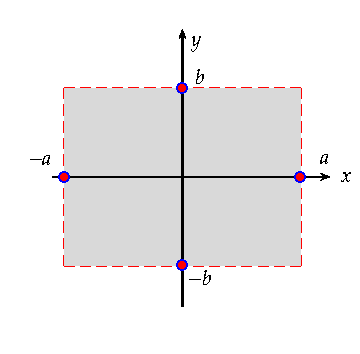
\includegraphics{retangulo-fundamental.pdf}
  % \psset{ticksize=0pt}
  % \begin{pspicture*}(-3,-3)(3,3)
  %   \psline[linestyle=dashed,linecolor=red](2,-1.5)(2,1.5)
  %   \psline[linestyle=dashed,linecolor=red](-2,-1.5)(-2,1.5)
  %   \psline[linestyle=dashed,linecolor=red](-2,1.5)(2,1.5)
  %   \psline[linestyle=dashed,linecolor=red](-2,-1.5)(2,-1.5)
  %   \pscustom[fillstyle=solid,fillcolor=gray!30,linestyle=none]
  %   {
  %     \psline(2,-1.5)(2,1.5)
  %     \psline(-2,-1.5)(-2,1.5)
  %     \psline(-2,1.5)(2,1.5)
  %     \psline(-2,-1.5)(2,-1.5)
  %   }
  %   \psaxes[labels=none]{->}(0,0)(-2.2,-2.2)(2.5,2.5)[$x$,0][$y$,-45]
  %   \psdot[linecolor=blue,fillcolor=red,dotstyle=o,dotsize=5pt](2,0)
  %   \rput(2.4,0.3){$a$}
  %   \psdot[linecolor=blue,fillcolor=red,dotstyle=o,dotsize=5pt](-2,0)
  %   \rput(-2.4,0.3){$-a$}
  %   \psdot[linecolor=blue,fillcolor=red,dotstyle=o,dotsize=5pt](0,1.5)
  %   \rput(0.3,1.7){$b$}
  %   \psdot[linecolor=blue,fillcolor=red,dotstyle=o,dotsize=5pt](0,-1.5)
  %   \rput(0.3,-1.7){$-b$}
  % \end{pspicture*}
\end{figure}
Esse ret\^angulo \'e chamado de \textbf{ret\^angulo fundamental} da elipse $\mathcal{E}$.\index{Elipse!Ret\^angulo Fundamental}

Agora, como $a > b$, ent\~ao
\[
  \dfrac{x^2}{a^2} + \dfrac{y^2}{a^2} \le \dfrac{x^2}{a^2} + \dfrac{y^2}{b^2} \le \dfrac{x^2}{b^2} + \dfrac{y^2}{b^2}.
\]
Assim, todo ponto $P(x,y)$ de $E$ satisfaz
\[
  \dfrac{x^2}{a^2} + \dfrac{y^2}{a^2} \le 1 \le \dfrac{x^2}{b^2} + \dfrac{y^2}{b^2}.
\]
e da{\'\i} $b^2 \le x^2 + y^2 \le a^2$, ou seja, $b \le d(P,O) \le a$. Portanto a elipse est\'a contida entre as circunfer\^encias de raio $a$ e $b$. Essa regi\~ao \'e chamada de \textbf{coroa fundamental} da elipse.\index{Elipse!Coroa Fundamental}
\begin{figure}[!h]
  \centering
  \caption{Coroa Fundamental}
  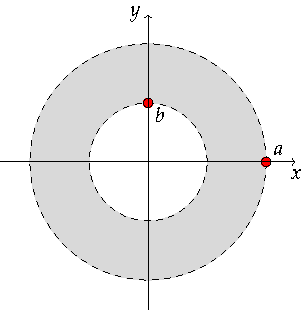
\includegraphics{coroa-fundamental.pdf}
  % \begin{tikzpicture}
  %   \coordinate (F) at (-2.5,0);
  %   \coordinate (G) at (0,-2.5);
  %   \coordinate (X) at (2.5,0);
  %   \coordinate (Y) at (0,2.5);
  %   \coordinate[label=right:$a$] (A) at (2,0.2);
  %   \coordinate[label=right:$b$] (B) at (0,0.8);
  %   % Styles
  %   \tikzstyle{axes}=[]

  %   \draw[fill=gray!30,even odd rule,style=dashed] (0,0) circle (2cm) circle (1cm) ;
  %   \draw[fill=red] (0,1) circle (0.08cm);
  %   \draw[fill=red] (2,0) circle (0.08cm);
  %   \begin{scope}[style=axes]%constr\'oi os eixos cartesianos
  %     \draw[->] (F) -- (X) node[below] {$x$} coordinate(x axis);
  %     \draw[->] (G) -- (Y) node[left] {$y$} coordinate(y axis);
  %   \end{scope}
  % \end{tikzpicture}
\end{figure}

Logo os pontos da elipse est\~ao na regi\~ao compreendida entre o ret\^angulo fundamental e a coroa fundamental.
\begin{figure}[!h]
  \centering
  \caption{Regi\~ao onde se encontram os pontos de uma elipse}
  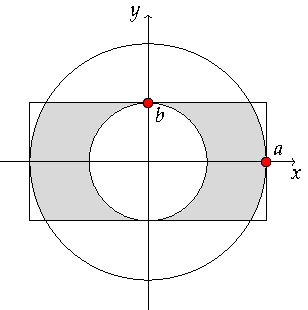
\includegraphics{regiao-fundamental.pdf}
  % \begin{tikzpicture}
  %   \coordinate (F) at (-2.5,0);
  %   \coordinate (G) at (0,-2.5);
  %   \coordinate (X) at (2.5,0);
  %   \coordinate (Y) at (0,2.5);
  %   \coordinate[label=right:$a$] (A) at (2,0.2);

  %   \begin{scope}
  %     \clip (-2,-1) rectangle (2,1);
  %     \fill[gray!30] (0,0) circle (2cm);
  %     \fill[white] (0,0) circle (1cm);
  %   \end{scope}

  %   \draw[name path=rf](-2,-1) rectangle (2,1);
  %   \draw[name path=cf2] (0,0) circle (2);
  %   \draw[name path=cf1] (0,0) circle (1cm);
  %   \coordinate[label=right:$b$] (B) at (0,0.8);
  %   \tikzstyle{axes}=[]
  %   \begin{scope}[style=axes]%constr\'oi os eixos cartesianos
  %     \draw[->] (F) -- (X) node[below] {$x$} coordinate(x axis);
  %     \draw[->] (G) -- (Y) node[left] {$y$} coordinate(y axis);
  %   \end{scope}
  %   \draw[fill=red] (0,1) circle (0.08cm);
  %   \draw[fill=red] (2,0) circle (0.08cm);
  % \end{tikzpicture}
\end{figure}
Assim observe que se $b/a$ estiver pr\'oximo de 1, ent\~ao o ret\^angulo fundamental ser\'a pr\'oximo de um quadrado e da{\'\i} a forma da elipse se aproximar\'a de um circunfer\^encia. Por outro lado, quanto mais pr\'oximo de 0 estiver $b/a$, mas alongada ser\'a a elipse. Mas, sabemos que
\[
  a^2 = b^2 + c^2
\]
da{\'\i}
\[
  \left(\dfrac{b}{a}\right)^2 + \left(\dfrac{c}{a}\right)^2 = 1.
\]
Dessa equa\c{c}\~ao vemos que se $b/a \to 1$, ent\~ao $c/a \to 0$ e da{\'\i} os focos de $\mathcal{E}$ est\~ao ``mais pr\'oximos'' de seu centro do que de seus v\'ertices e desse modo a elipse ser\'a mais parecida com um circunfer\^encia. Por outro lado, se $b/a \to 0$, ent\~ao $c/a \to 1$ e assim os focos de $\mathcal{E}$ est\~ao ``mais pr\'oximos'' dos v\'ertices do que do centro de $\mathcal{E}$ e desse modo a elipse ser\'a mais alongada.  Portanto o quociente $c/a$ mede o quanto os focos de $\mathcal{E}$ est\~ao ``fora do centro''. A essa raz\~ao damos o nome de \textbf{excentricidade} (\textit{ex centrum}) da elipse e representamos por\index{Elipse!Excentricidade}
\[
  e = \dfrac{c}{a}.
\]

% subsection elipse (end)

\subsection{Hip\'erbole} % (fold)
\label{sub:hiperbole}

\begin{definicao}
  Sejam $F_1$ e $F_2$ pontos distintos do plano tais que sua dist\^ancia seja $2c$. Considere um n\'umero real $a$ tal que $0 < a < c$. O lugar geom\'etrico $\mathcal{H}$ dos pontos $P(x,y)$ tais que 
  \begin{equation}\label{equacaohiperbole}
    | d(P,F) - d(P,F_2)| = 2a
  \end{equation}
  chama-se \textbf{hip\'erbole}. Os pontos $F_1$ e $F_2$ s\~ao chamados \textbf{focos} da hip\'erbole, o segmento $F_1F_2$ \'e chamado \textbf{segmento focal}, o ponto m\'edio do segmento $F_1F_2$ \'e chamada de \textbf{centro} da hip\'erbole e o n\'umero $2c$ \'e chamado de \textbf{dist\^ancia focal}. A reta passando por $F_1$ e $F_2$ \'e chamada \textbf{reta focal}.\index{Hip\'erbole} \index{Hip\'erbole!Focos} \index{Hip\'erbole!Segmento Focal} \index{Hip\'erbole!Centro} \index{Hip\'erbole!Dist\^ancia Focal} \index{Hip\'erbole!Reta Focal}
\end{definicao}

Vamos fixar $F_1(-c,0)$ e $F_2(c,0)$. Assim um ponto $P(x,y)$ pertence \`a hip\'erbole $\mathcal{H}$ de focos $F_1$ e $F_2$ se
\begin{align*}
  &| d(P,F_1) - d(P,F_2) | = 2a\\
  &d(P,F_1) - d(P,F_2) = \pm 2a\\
  &d(P,F_1) = \pm 2a + d(P,F_2)\\
  &\left[\sqrt{(x + c)^2 + y^2}\right]^2 = \left[\pm 2a + \sqrt{(x - c)^2 + y^2}\right]^2\\
  &(cx - a^2)^2 = \left[\pm a\sqrt{(x - c)^2 + y^2}\right]^2\\
  &(c^2 - a^2)x^2 - a^2y^2 = a^2(c^2 - a^2).
\end{align*}
Fazendo $b^2 = c^2 - a^2$ e dividindo por $a^2b^2$ obtemos
\begin{equation}
  \dfrac{x^2}{a^2} - \dfrac{y^2}{b^2} = 1
\end{equation}
Como no caso da elipse, tamb\'em temos as rela\c{c}\~oes
\begin{align}
  c^2 = a^2 + b^2\\
  c > b > 0\label{pitagorashiperbole}\\
  c > a > 0.
\end{align}
Portanto, se um ponto $P(x,y)$ pertence \`a hip\'erbole $\mathcal{H}$, ent\~ao ele satisfaz a equa\c{c}\~ao \eqref{equacaohiperbole}.

Agora, dado um ponto $A(\alpha,\beta)$ que satisfaz a equa\c{c}\~ao \eqref{equacaohiperbole}, queremos mostrar que $A$ pertence \`a hip\'erbole $\mathcal{H}$. Temos
\begin{align}
  \dfrac{\alpha^2}{a^2} - \dfrac{\beta^2}{b^2} = 1\nonumber\\
  \beta^2 = \dfrac{b^2}{a^2}\alpha^2 - b^2.\label{equacaoauxiliarhiperbole}
\end{align}
Usando \eqref{pitagorashiperbole} e \eqref{equacaoauxiliarhiperbole}:
\begin{align*}
  d^2(P,F_1) &= (\alpha + c)^2 + \beta^2\\
  &= \alpha^2 + 2\alpha c + cˆ2 + \dfrac{b^2}{a^2}\alpha^2 - b^2
\end{align*}
donde
\[
  d^2(A,F_1) = \left(\dfrac{c}{a}\alpha + a\right)^2.
\]
Do mesmo modo, obtemos
\[
  d^2(A,F_2) = \left(\dfrac{c}{a}\alpha - a\right)^2.
\]
Assim
\begin{align}
  d(A,F_1) = \left|\dfrac{c}{a}\alpha + a\right|\\
  d(A,F_2) = \left|\dfrac{c}{a}\alpha - a\right|.
\end{align}

Mas
\[
  \dfrac{\alpha^2}{a^2} - \dfrac{\beta^2}{b^2} = 1
\]
assim 
\begin{equation}\label{pontohiperbole}
  \alpha^2/a^2 \ge 1,
\end{equation}
isto \'e, $\alpha \le -a$ ou $\alpha \ge a$. Temos ent\~ao dois casos para analisar:
\begin{enumerate}
  \item Se $\alpha \le -a$, ent\~ao
  \[
    \dfrac{c}{a}\alpha \le -c < -a.
  \]
  Portanto, $(c/a)\alpha + a < 0$ e $(c/a)\alpha - a < 0$, donde
  \begin{align*}
  d(A,F_1) = -\dfrac{c}{a}\alpha - a\\
  d(A,F_2) = -\dfrac{c}{a}\alpha + a.
\end{align*}
e ent\~ao
\[
  | d(P,F_1) - d(P,F_2)| = |-2a| = 2a.
\]
\item Se $\alpha \ge -a$, ent\~ao
  \[
    \dfrac{c}{a}\alpha \le c > a.
  \]
  Portanto, $(c/a)\alpha + a > 0$ e $(c/a)\alpha - a > 0$, donde
  \begin{align*}
  d(A,F_1) = \dfrac{c}{a}\alpha + a\\
  d(A,F_2) = \dfrac{c}{a}\alpha - a.
\end{align*}
e ent\~ao
\[
  | d(P,F_1) - d(P,F_2)| = |2a| = 2a.
\]
\end{enumerate}
Portanto, se $A(\alpha,\beta)$ satisfaz a equa\c{c}\~ao \eqref{equacaohiperbole}, ent\~ao $A$ pertence \`a hip\'erbole de focos $F_1(-c,0)$ e $F_2(c,0)$. Assim provamos a seguinte proposi\c{c}\~ao:

\begin{proposicao}
  Um ponto $P(x, y)$ \'e um ponto da hip\'erbole
  \[
    \mathcal{H}:\ \dfrac{x^2}{a^2} - \dfrac{y^2}{b^2} = 1
  \]
  se, e somente se, as dist\^ancias de $P$ aos focos s\~ao:
  \begin{align*}
    d(A,F_1) = \left|\dfrac{c}{a}\alpha + a\right|\\
    d(A,F_2) = \left|\dfrac{c}{a}\alpha - a\right|.
  \end{align*}
\end{proposicao}

Os n\'umeros $a$, $b$ e $c$ s\~ao chamados \textbf{par\^ametros geom\'etricos} da hip\'erbole $\mathcal{H}$ e a equa\c{c}\~ao
\[
  \dfrac{x^2}{a^2} - \dfrac{y^2}{b^2} = 1
\]
\'e chamada de \textbf{equa\c{c}\~ao reduzida} da hip\'erbole.\index{Hip\'erbole!Par\^ametros Geom\'etricos} \index{Hip\'erbole!Equa\c{c}\~ao Reduzida}

\begin{observacao}
  Seja $\mathcal{H} : \dfrac{x^2}{a^2} - \dfrac{y^2}{b^2} = 1$ uma hip\'erbole de focos no eixo $x$.
  \begin{enumerate}
    \item Nenhum ponto $P(x,y)$ de $\mathcal{H}$ \'e tal que $-a < x < a$, pois caso contr\'ario ter{\'\i}amos $x^2 < a^2$ o que contradiz a inequa\c{c}\~ao \eqref{pontohiperbole}. Para a ordenada $y$ n\~ao h\'a restri\c{c}\~ao, isto \'e, qualquer que seja $y$ existe $x$ tal que $\dfrac{x^2}{a^2} - \dfrac{y^2}{b^2} = 1$. Assim a hip\'erbole n\~ao \'e limitada.
    \item Se $(x,y)$ pertence a $H$, ent\~ao $(-x,-y)$, $(x,-y)$ e $(-x,y)$ tamb\'em pertencem a $\mathcal{H}$. Logo a hip\'erbole \'e sim\'etrica em rela\c{c}\~ao ao eixo $x$, ao eixo $y$  e em rela\c{c}\~ao \`a origem do plano cartesiano.
    \item O ponto $(x,0)$ pertence \`a hip\'erbole $\mathcal{H}$ se, e s\'o se, $x = \pm a$. Por isso a interse\c{c}\~ao de $\mathcal{H}$ com a reta focal s\~ao os pontos $A_1(-a,0)$ e $A_2(a,0)$, chamados de \textbf{v\'ertices} de $\mathcal{H}$.\index{Hip\'erbole!V\'ertices}
  \end{enumerate}
\end{observacao}

Considere a hip\'erbole $\mathcal{H}$ de equa\c{c}\~ao reduzida
\[
  \mathcal{H} : \dfrac{x^2}{a^2} - \dfrac{y^2}{b^2} = 1
\]
com focos $F_1(-c,0)$ e $F_2(c,0)$. Dada uma reta $r$ de equa\c{c}\~ao $y = mx$, quais as condi\c{c}\~oes sobre $a$, $b$, $c$ e $m$ para que a reta $r$ intercepte $\mathcal{H}$?

Seja $P(x_0,y_0)$ um ponto de interse\c{c}\~ao entre $r$ e $\mathcal{H}$. Ent\~ao temos
\begin{align*}
  \dfrac{x_0^2}{a^2} - \dfrac{y_0^2}{b^2} = 1\\
  y_0 = mx_0,
\end{align*}
isto \'e,
\[
  \dfrac{x_0^2}{a^2} - \dfrac{m^2x_0^2}{b^2} = 1.
\]
Resolvendo em $x_0$ obtemos
\begin{equation}\label{intersecaohiperbolereta}
x_0 = \pm \dfrac{ab}{\sqrt{b^2 - a^2m^2}} = \pm \dfrac{b}{\sqrt{\dfrac{b^2}{a^2} - m^2}}.
\end{equation}
Assim
\[
  b^2 - a^2m^2 > 0 \Leftrightarrow m^2 < \dfrac{b^2}{a^2}.
\]
Como $a$ e $b$ s\~ao positivos
\[
  -\dfrac{b}{a} < m < \dfrac{b}{a}.
\]
Logo a reta $y = mx$ intercepta a hip\'erbole $\mathcal{H}$ se, e s\'o se, seu coeficiente angular est\'a entre $-b/a$ e $b/a$. Portanto as retas
\[
  y = -\dfrac{b}{a}x \quad \mbox{e}\quad y = \dfrac{b}{a}x
\]
n\~ao interceptam a hip\'erbole $\mathcal{H}$. Tais retas s\~ao chamadas de \textbf{ass{\'\i}ntotas da hip\'erbole}. Mais ainda, da equa\c{c}\~ao \eqref{intersecaohiperbolereta} quando $m \to b/a$, o ponto $x_0$ tende para mais ou menos infinito. Logo os pontos da hip\'erbole se aproximam das ass{\'\i}ntotas a medida que $x$ se afasta da origem.\index{Hip\'erbole!Ass{\'\i}ntotas}

Como no caso da elipse, utilizando a simetria e as ass{\'\i}ntodas da hip\'erbole, podemos mostrar a partir da equa\c{c}\~ao
\[
  y = \dfrac{b}{a}\sqrt{x^2 - a^2}, \quad x \ge a
\]
que a forma da hip\'erbole ser\'a dada pela Figura \ref{FormageralHiperbole}.
\begin{figure}[!h]
  \centering
  \caption{Hip\'erbole $\dfrac{x^2}{a^2} - \dfrac{y^2}{b^2} = 1$  com ass{\'\i}ntotas $y = -\dfrac{b}{a}x$ e $y = \dfrac{b}{a}x$}
  \label{FormageralHiperbole}
  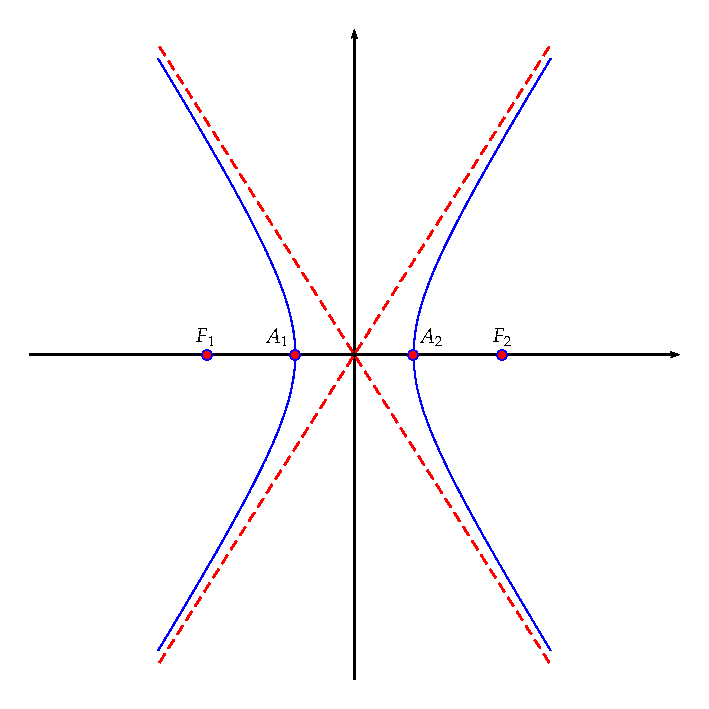
\includegraphics{hiperbole-focos-eixo-X.pdf}
  % \psset{ticksize=0pt}
  % \begin{pspicture*}(-6,-6)(6,6)
  %   \psaxes[labels=none]{->}(0,0)(-5.5,-5.5)(5.5,5.5)
  %   \psplot[algebraic,linestyle=dashed,linecolor=red]{-3.3}{3.3}{-1.58*x}
  %   \psplot[algebraic,linestyle=dashed,linecolor=red]{-3.3}{3.3}{1.58*x}
  %   \psplotImp[algebraic,linecolor=blue,stepFactor=0.1,linewidth=0.5pt](-5,-5)(5,5){x^2-y^2/2.5-1}
  %   \rput(1.3,0.3){$A_2$}
  %   \rput(-1.3,0.3){$A_1$}
  %   \rput(2.5,0.3){$F_2$}
  %   \rput(-2.5,0.3){$F_1$}
  %   \psdot[linecolor=blue,fillcolor=red,dotstyle=o,dotsize=5pt](-1,0)
  %   \psdot[linecolor=blue,fillcolor=red,dotstyle=o,dotsize=5pt](1,0)
  %   \psdot[linecolor=blue,fillcolor=red,dotstyle=o,dotsize=5pt](-2.5,0)
  %   \psdot[linecolor=blue,fillcolor=red,dotstyle=o,dotsize=5pt](2.5,0)
  % \end{pspicture*}
\end{figure}

\begin{proposicao}
  Um equa\c{c}\~ao da forma
  \begin{equation}\label{hiperbolegeral}
    \dfrac{x^2}{p} + \dfrac{y^2}{q} = 1
  \end{equation}
  descreve uma hip\'erbole se, e somente se, os n\'umeros reais $p$ e $q$ s\~ao de sinal contr\'ario.
\end{proposicao}

\begin{corolario}
  Sejam $p$ e $q$ n\'umeros reais de sinal contr\'ario e $\mathcal{H}$ a hip\'erbole de equa\c{c}\~ao \eqref{hiperbolegeral} e par\^ametros geom\'etricos $a$ e $b$.
  \begin{enumerate}
    \item Se $p > 0$ e $q < 0$, ent\~ao $a^2 = p$ e $b^2 = -q$, $\mathcal{H}$ tem centro na origem, focos no eixo $x$ e ass{\'\i}ntotas dadas por $y = \pm(b/a)x$.
    \item Se $p < 0$ e $q > 0$, ent\~ao $a^2 = q$ e $b^2 = -p$, $\mathcal{H}$ tem centro na origem, focos no eixo $y$ e ass{\'\i}ntotas dadas por $x = \pm(a/b)y$.
  \end{enumerate}
\end{corolario}

\begin{exemplos}
  \begin{enumerate}
    \item Encontre a equa\c{c}\~ao da hip\'erbole cujos v\'ertices s\~ao $(-15,0)$ e $(15,0)$ e as ass{\'\i}ntotas t\^em equa\c{c}\~oes $5y - 4x = 0$ e $5y + 4x = 0$.
    \begin{solucao}
      As ass{\'\i}ntotas s\~ao dadas por
      \[
        y = -\dfrac{b}{a}x \quad\mbox{e }\quad y = \dfrac{b}{a}x.
      \]
      A partir dos v\'ertices encontramos $a = 15$. Da{\'\i} $b = 12$ e ent\~ao a equa\c{c}\~ao da hip\'erbole \'e
      \[
        \dfrac{x^2}{225} - \dfrac{y^2}{144} = 1.
      \]
    \end{solucao}
    \item Encontre a equa\c{c}\~ao da hip\'erbole de focos $F_1(0,-\sqrt{20})$ e $F_1(0,\sqrt{20})$ e tal que $a = 2$.
    \begin{solucao}
      Como os focos n\~ao est\~ao no eixo $x$, vamos usar a equa\c{c}\~ao \eqref{equacaohiperbole}:
      \begin{align*}
        &\mid d(P,F) - d(P,F_2)\mid = 4\\
        &\left[\sqrt{x^2 + (y + \sqrt{20})^2}\right]^2 = \left[\pm 4 + \sqrt{x^2 + (y - \sqrt{20})^2}\right]^2\\
        &(y\sqrt{20} - 4)^2 = \left[\pm 2\sqrt{x^2 + (y - \sqrt{20})^2}\right]^2\\
        &20y^2 - 8\sqrt{20}y + 16 = 4x^2 + 4y^2 - 8\sqrt{20}y + 80\\
        &16y^2 - 4x^2 = 64.
      \end{align*}
      Logo a hip\'erbole procurada tem equa\c{c}\~ao
      \[
        \dfrac{y^2}{4} - \dfrac{x^2}{16} = 1.
      \]
      Portanto as ass{\'\i}ntotas s\~ao
      \[
        y = -2x \quad\mbox{e }\quad y = 2x.
      \]
    \end{solucao}
  \end{enumerate}
\end{exemplos}

% \begin{observacao}
%   No caso de uma hip\'erbole $\mathcal{H}$ com focos no eixo $y$, isto \'e, com equa\c{c}\~ao
%   \[
%     \mathcal{H}: \dfrac{y^2}{a^2} - \dfrac{x^2}{b^2} = 1
%   \]
%   as ass{\'\i}ntotas ter\~ao equa\c{c}\~oes dadas por
%   \[
%     x = \pm \dfrac{a}{b}y.
%   \]
% \end{observacao}

\begin{figure}[h]
  \centering
  \caption{Hip\'erbole $\dfrac{y^2}{b^2} - \dfrac{x^2}{a^2} = 1$ com ass{\'\i}ntotas $x = -\dfrac{a}{b}y$ e $x = \dfrac{a}{b}y$}
  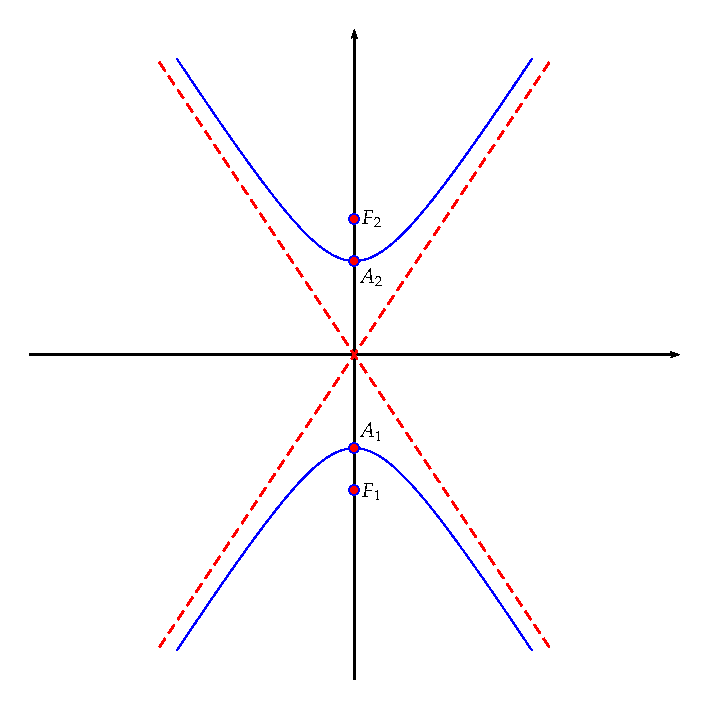
\includegraphics{hiperbole-focos-eixo-Y.pdf}
  % \psset{ticksize=0pt}
  % \begin{pspicture*}(-6,-6)(6,6)
  %   \psaxes[labels=none]{->}(0,0)(-5.5,-5.5)(5.5,5.5)
  %   \psplot[algebraic,linestyle=dashed,linecolor=red]{-3.3}{3.3}{-1.5*x}
  %   \psplot[algebraic,linestyle=dashed,linecolor=red]{-3.3}{3.3}{1.5*x}
  %   \psplotImp[algebraic,linecolor=blue,stepFactor=0.1,linewidth=0.5pt](-5,-5)(5,5){y^2/2.5 - x^2-1}
  %   \rput(0.3,1.3){$A_2$}
  %   \rput(0.3,-1.3){$A_1$}
  %   \rput(0.3,2.3){$F_2$}
  %   \rput(0.3,-2.3){$F_1$}
  %   \psdot[linecolor=blue,fillcolor=red,dotstyle=o,dotsize=5pt](0,-1.58)
  %   \psdot[linecolor=blue,fillcolor=red,dotstyle=o,dotsize=5pt](0,1.58)
  %   \psdot[linecolor=blue,fillcolor=red,dotstyle=o,dotsize=5pt](0,-2.3)
  %   \psdot[linecolor=blue,fillcolor=red,dotstyle=o,dotsize=5pt](0,2.3)
  % \end{pspicture*}
\end{figure}

% subsection hiperbole (end)



\subsection{Par\'abola} % (fold)
\label{sub:parabolas}

\begin{definicao}
  Seja $r$ uma reta e $F$ um ponto que n\~ao pertence a $r$. O lugar geom\'etrico $\mathcal{P}$ dos pontos equidistantes de $F$ e $r$ chama-se \textbf{par\'abola}. O ponto $F$ \'e chamado de \textbf{foco da par\'abola} e $r$ de \textbf{reta diretriz}.\index{Par\'abola} \index{Par\'abola!Focos} A reta contendo o foco $F$ e perpendicular \`a reta diretriz \'e chamada de \textbf{reta focal}.\index{Par\'abola!Reta diretriz}\index{Par\'abola!Reta focal}
\end{definicao}


Vamos fixar $F(p,0)$ e $r: x = -p$, onde $p > 0$. Assim um ponto $A(x,y)$ pertence \`a par\'abola de foco $F$ e reta diretriz $r$ se, e somente se,
\begin{figure}[!h]%par\'abola
  \centering
  \caption{Defini\c{c}\~ao da Par\'abola}
  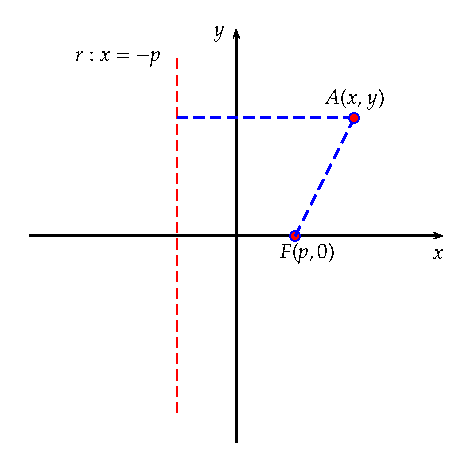
\includegraphics{parabola.pdf}
  % \psset{ticksize=0pt}
  % \begin{pspicture*}(-4,-4)(4,4)
  %   \psaxes[labels=none]{->}(0,0)(-3.5,-3.5)(3.5,3.5)
  %   \psline[linestyle=dashed,linecolor=red](-1,-3)(-1,3)
  %   \rput(1.2,-0.3){$F(p,0)$}
  %   \psdot[linecolor=blue,fillcolor=red,dotstyle=o,dotsize=5pt](1,0)
  %   \rput(2,2.3){$A(x,y)$}
  %   \psline[linestyle=dashed,linecolor=blue](1,0)(2,2)
  %   \psline[linestyle=dashed,linecolor=blue](-1,2)(2,2)
  %   \psdot[linecolor=blue,fillcolor=red,dotstyle=o,dotsize=5pt](2,2)
  %   \rput(-2,3){$r: x = -p$}
  %   \rput(3.4,-0.3){$x$}
  %   \rput(-0.3,3.4){$y$}
  % \end{pspicture*}
\end{figure}

\[
  d(A,r) = d(A,F).
\]
Mas
\begin{align*}
  d(A,r) = |x + p|\\
  d(A,F) = \sqrt{(x - p)^2 + y^2}.
\end{align*}
Logo $A$ pertence \`a par\'abola $\mathcal{P}$ se, e somente se,
\begin{align*}
  (|x + p|)^2 = (x - p)^2 + y^2\\
  x^2 + 2px + p^2 = x^2 - 2px + p^2 + y^2.
\end{align*}
Portanto $A(x,y)$ pertence \`a par\'abola $\mathcal{P}$ se, e somente se,
\begin{equation}\label{equacaoparabola}
  y^2 = 4px
\end{equation}

A equa\c{c}\~ao \eqref{equacaoparabola} \'e chamada de \textbf{equa\c{c}\~ao reduzida} da par\'abola $\mathcal{P}$. Indica-se\index{Par\'abola!Equa\c{c}\~ao reduzida}
\[
  \mathcal{P}:\ y^2 = 4px.
\]

\begin{observacao}
  \begin{enumerate}
    \item Se $(x,y)$ satisfaz a equa\c{c}\~ao \eqref{equacaoparabola}, ent\~ao $x \ge 0$, isto \'e, nenhum ponto de $\mathcal{P}$ tem abscissa negativa. J\'a para a ordenada $y$, n\~ao existem restri\c{c}\~oes. Logo a par\'abola n\~ao \'e limitada.
    \item Se $(x,y)$ pertence a $\mathcal{P}$, ent\~ao $(x,-y)$ tamb\'em pertence a $\mathcal{P}$. Logo a par\'abola \'e sim\'etrica em rela\c{c}\~ao ao eixo $x$.
    \item O \'unico ponto de interse\c{c}\~ao de $\mathcal{P}$ com os eixos coordenados \'e o ponto $(0,0)$. Tal ponto \'e chamado de \textbf{v\'ertice} da par\'abola.\index{Par\'abola!V\'ertice}
  \end{enumerate}
\end{observacao}

Na equa\c{c}\~ao \eqref{equacaoparabola} podemos isolar $x$ e escrever
\[
  x = \dfrac{y^2}{4p}
\]
obtendo assim $x$ como uma fun\c{c}\~ao de $y$. Logo o gr\'afico da par\'abola $\mathcal{P}$ \'e:

\begin{figure}[!h]%par\'abola
  \centering
  \caption{Par\'abola $\mathcal{P}: y^2 = 4px$ e reta diretriz $r: x = -p$, $p > 0$}
  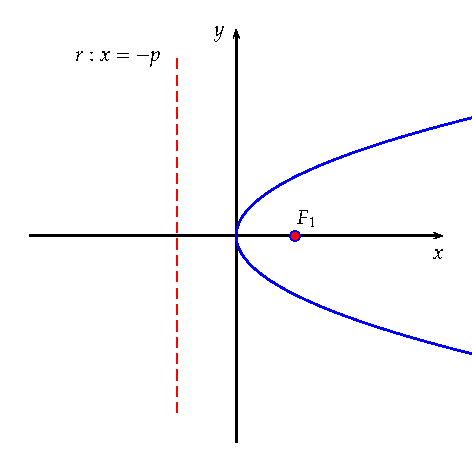
\includegraphics{parabola-foco-eixo-X-positivo.pdf}
  % \psset{ticksize=0pt}
  % \begin{pspicture*}(-4,-4)(4,4)
  %   \psaxes[labels=none]{->}(0,0)(-3.5,-3.5)(3.5,3.5)
  %   \rput{-90}(0,0){
  %     \psplot[algebraic,linecolor=blue
  %     ]{-2.0}{2.0}{x^2}
  %   }
  %   \psline[linestyle=dashed,linecolor=red](-1,-3)(-1,3)
  %   \rput(1.2,0.3){$F_1$}
  %   \psdot[linecolor=blue,fillcolor=red,dotstyle=o,dotsize=5pt](1,0)
  %   \rput(-2,3){$r: x = -p$}
  %   \rput(3.4,-0.3){$x$}
  %   \rput(-0.3,3.4){$y$}
  % \end{pspicture*}
\end{figure}

Agora, se a diretriz de $\mathcal{P}$ tem equa\c{c}\~ao $r: x = p$ e o foco \'e o ponto $F(-p,0)$, com $p > 0$, obtemos a equa\c{c}\~ao
\[
  y^2 = -4px.
\]
Neste caso, o gr\'afico da par\'abola \'e dado pela Figura \ref{FormageralParabola}.
\begin{figure}[!h]%par\'abola
  \centering
  \caption{Par\'abola $\mathcal{P}: y^2 = -4px$ e reta diretriz $r: x = p$, $p > 0$}
  \label{FormageralParabola}
  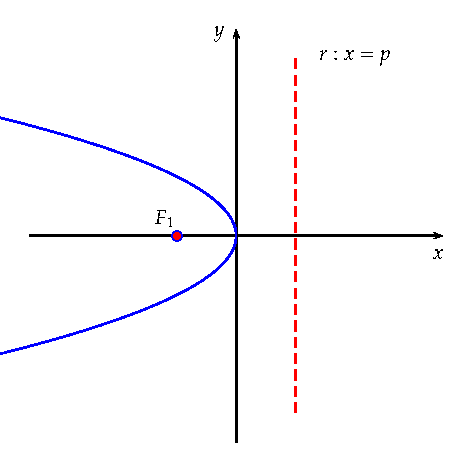
\includegraphics{parabola-foco-eixo-X-negativo.pdf}
  % \psset{ticksize=0pt}
  % \begin{pspicture*}(-4,-4)(4,4)
  %   \psaxes[labels=none]{->}(0,0)(-3.5,-3.5)(3.5,3.5)
  %   \rput{90}(0,0){
  %     \psplot[algebraic,linecolor=blue
  %     ]{-2.0}{2.0}{x^2}
  %   }
  %   \rput(-1.2,0.3){$F_1$}
  %   \psdot[linecolor=blue,fillcolor=red,dotstyle=o,dotsize=5pt](-1,0)
  %   \psline[linestyle=dashed,linecolor=red](1,-3)(1,3)
  %   \rput(2,3){$r: x = p$}
  %   \rput(3.4,-0.3){$x$}
  %   \rput(-0.3,3.4){$y$}
  % \end{pspicture*}
\end{figure}

Nos demais casos temos:
\begin{figure}[!h]%par\'abola
  \centering
  \caption{Par\'abola $\mathcal{P}: x^2 = -4py$ e reta diretriz $r: y = p$, $p > 0$}
  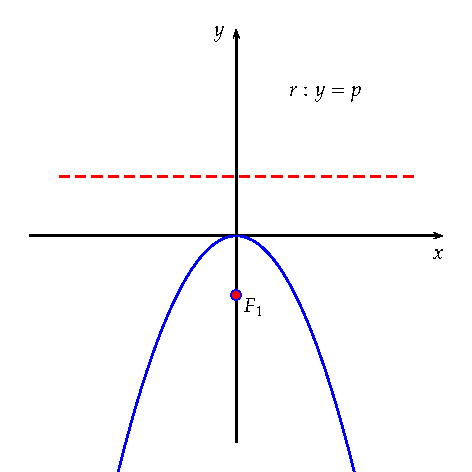
\includegraphics{parabola-foco-eixo-Y-negativo.pdf}
  % \psset{ticksize=0pt}
  % \begin{pspicture*}(-4,-4)(4,4)
  %   \psaxes[labels=none]{->}(0,0)(-3.5,-3.5)(3.5,3.5)
  %     \psplot[algebraic,linecolor=blue
  %     ]{-2.0}{2.0}{-x^2}
  %   \rput(0.3,-1.2){$F_1$}
  %   \psdot[linecolor=blue,fillcolor=red,dotstyle=o,dotsize=5pt](0,-1)
  %   \psline[linestyle=dashed,linecolor=red](-3,1)(3,1)
  %   \rput(1.5,2.4){$r: y = p$}
  %   \rput(3.4,-0.3){$x$}
  %   \rput(-0.3,3.4){$y$}
  % \end{pspicture*}
\end{figure}

\begin{figure}[!h]%par\'abola
  \centering
  \caption{Par\'abola $\mathcal{P}: x^2 = 4py$ e reta diretriz $r: y = -p$, $p > 0$}
  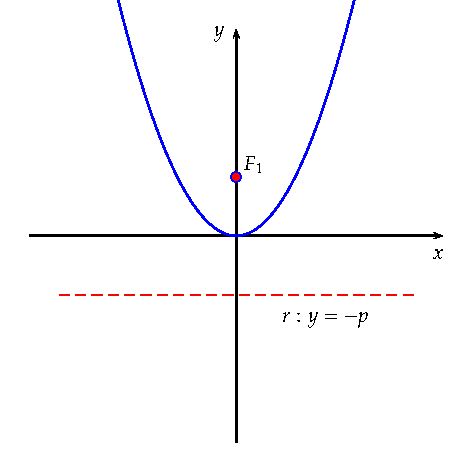
\includegraphics{parabola-foco-eixo-Y-positivo.pdf}
  % \psset{ticksize=0pt}
  % \begin{pspicture*}(-4,-4)(4,4)
  %   \psaxes[labels=none]{->}(0,0)(-3.5,-3.5)(3.5,3.5)
  %     \psplot[algebraic,linecolor=blue
  %     ]{-2.0}{2.0}{x^2}
  %   \rput(0.3,1.2){$F_1$}
  %   \psdot[linecolor=blue,fillcolor=red,dotstyle=o,dotsize=5pt](0,1)
  %   \psline[linestyle=dashed,linecolor=red](-3,-1)(3,-1)
  %   \rput(1.5,-1.4){$r: y = -p$}
  %   \rput(3.4,-0.3){$x$}
  %   \rput(-0.3,3.4){$y$}
  % \end{pspicture*}
\end{figure}

\begin{proposicao}
  As equa\c{c}\~oes $y^2 = qx$ e $x^2 = qy$ descrevem uma par\'abola se, e somente se, $q \ne 0$.
\end{proposicao}
% subsection parabolas (end)
% section conicas (end)

\section{Rota\c{c}\~ao e Transla\c{c}\~ao de Eixos} % (fold)
\label{sec:rotacao_e_translacao_de_eixos}


Para determinar a c\^onica representada pela equa\c{c}\~ao
\[
  g(x, y) = ax^2 + bxy + cy^2 + dx + ey + f = 0
\]
iremos utilizar transla\c{c}\~oes e rota\c{c}\~oes de eixos para simplificar sua equa\c{c}\~ao.

\subsection{Transla\c{c}\~ao de eixos} % (fold)
\label{sub:translacaoo_de_eixos}
Considere a seguinte c\^onica
\begin{equation}\label{conicaexemplo}
  x^2 + 2y^2 - 4x - 4y - 1 = 0.
\end{equation}
Podemos escrever
\begin{align*}
  &(x^2 - 4x + 4) - 4 + 2(y^2 - 2y + 1 - 1) - 1 = 0\\
  &(x - 2)^2 - 4 + 2(y - 1)^2 - 2 - 1 = 0\\
  &(x - 2)^2 + 2(y - 1)^2 = 7.
\end{align*}
Fazendo a mudan\c{c}a
\begin{align}
  x - 2 = x_1\label{mudancaX}\\
  y - 1 = y_1\label{mudancaY}
\end{align}
obtemos
\[
  \dfrac{x_1^2}{7} + \dfrac{y_1^2}{\dfrac{7}{2}} = 1
\]
que representa uma elipse com focos no eixo $x_1$.

O efeito das equa\c{c}\~oes \eqref{mudancaX} e \eqref{mudancaY} foi o de mudar o centro da elipse de equa\c{c}\~ao \eqref{conicaexemplo} que estava no ponto $(2,1)$ no sistema original para o ponto $(0,0)$ considerando os eixos coordenados $x_1$ e $y_1$. 

Utilizando-se as equa\c{c}\~oes \eqref{mudancaX} e \eqref{mudancaY} podemos facilmente escrever as coordenadas de um ponto $P$ qualquer, tanto em rela\c{c}\~ao ao sistema de eixos coordenados $x$ e $y$, quanto ao sistema de eixos coordenados $x_1$ e $y_1$. Por exemplo, o ponto $P$ de coordenadas $P = (4,0)$, em rela\c{c}\~ao ao sistema $xy$, ter\'a coordenadas $(2,-1)$ em rela\c{c}\~ao ao sistema de eixos $x_1y_1$. As mudan\c{c}as introduzidas pelas equa\c{c}\~oes \eqref{mudancaX} e \eqref{mudancaY} s\~ao chamadas de \textbf{transla\c{c}\~oes de eixos}. De modo geral, se $(x,y)$ s\~ao as coordenadas de um ponto $P$ em rela\c{c}\~ao ao ponto $(0,0)$, ent\~ao as coordenadas de $P$ em rela\c{c}\~ao aos eixos $x_1$ e $y_1$, centrados no ponto $(\alpha,\beta)$ s\~ao dadas por\index{Transla\c{c}\~ao de Eixos}
\begin{align}
  x_1 = x - \alpha\label{mudancaXgeral}\\
  y_1 = y - \beta\label{mudancaYgeral}.
\end{align}

\begin{figure}[!h]
  \centering
  \caption{Transla\c{c}\~ao de eixos}
  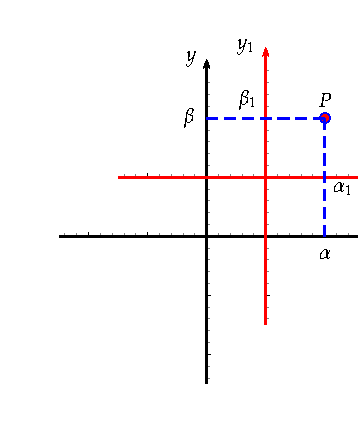
\includegraphics{translacao-eixos.pdf}
  % \begin{minipage}[b]{0.5\linewidth}
  %   \psset{ticksize=2pt}
  %   \begin{pspicture*}(-3.5,-3.5)(4,4)
  %     \psaxes[subticks=5,labels=none]{->}(0,0)(-2.5,-2.5)(3,3)[$x$,0][$y$,-180]
  %     \rput(2,-0.3){$\alpha$}
  %     \rput(-0.3,2){$\beta$}
  %     \psaxes[subticks=5,labels=none,linecolor=red]{->}(1,1)(-1.5,-1.5)(3.5,3.2)[$x_1$,0][$y_1$,-180]
  %     \rput(2.3,0.8){$\alpha_1$}
  %     \rput(0.7,2.3){$\beta_1$}
  %     \rput(2,2.3){$P$}
  %     \psdot[linecolor=blue,fillcolor=red,dotstyle=o,dotsize=5pt](2,2)
  %     \psline[linestyle=dashed,linecolor=blue](2,0)(2,2)
  %     \psline[linestyle=dashed,linecolor=blue](0,2)(2,2)
  %   \end{pspicture*}
  % \end{minipage}
\end{figure}
As mudan\c{c}as introduzidas pelas equa\c{c}\~oes \eqref{mudancaXgeral} e \eqref{mudancaYgeral} permitem remover os termos lineares da equa\c{c}\~ao \eqref{equacaoconica}.

\begin{exemplos}
  Identifique as c\^onicas:
  \begin{enumerate}
    \item $4x^2 - 8x + 9y^2 - 36y + 4 = 0$
    \begin{solucao}
      Completando quadrados
      \begin{align*}
        &4(x^2 - 2x + 1 - 1) + 9(y^2 - 4y + 4 - 4) + 4 = 0\\
        &4(x - 1)^2 + 9(y - 2)^2 = 36.
      \end{align*}
      Fazendo
      \begin{align*}
        x - 1 = x_1\\
        y - 2 = y_1
      \end{align*}
      obtemos
      \[
        \dfrac{x_1^2}{9} + \dfrac{y_1^2}{4} = 1
      \]
      que representa uma elipse com focos no eixo $x_1$. No novo sistema de coordenadas centrado no ponto os v\'ertices s\~ao
      \begin{align*}
        \overline{A_1}(-3,0),\quad \overline{A_2}(3,0)\\
        \overline{B_1}(0,-2),\quad \overline{B_2}(0,2).
      \end{align*}
      No sistema original os v\'ertices s\~ao
      \begin{align*}
        A_1(-2,2),\quad A_2(2,2)\\
        B_1(1,0),\quad B_2(1,4).
      \end{align*}
       \begin{figure}[!h]
        \centering
        \caption{Elipse $4x^2 - 8x + 9y^2 - 36y + 4 = 0$}
        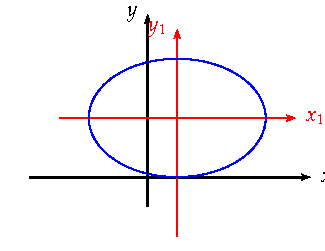
\includegraphics{elipse-eixos-tranladados.pdf}
        % \psset{unit=0.5cm}
        % \psset{ticksize=0pt}
        % \begin{pspicture*}(-5,-2.5)(6,6)
        %   \psaxes[labels=none]{->}(0,0)(-4,-1)(5.5,5.5)[$x$,0][$y$,-180]
        %   \psaxes[labels=none,linecolor=red]{->}(1,2)(-3,-2)(5,5)[$\color{red} x_1$,0][$\color{red} y_1$,-180]
        %   \psplotImp[algebraic,linecolor=blue,stepFactor=0.1,linewidth=0.5pt](-4,-1)(6,7){4*x^2 - 8*x + 9*y^2 - 36*y + 4}
        % \end{pspicture*}
      \end{figure}
    \end{solucao}
    \item $x^2 - 2y^2 - 6x - 8y - 1 = 0$
    \begin{solucao}
      Completando quadrados
      \begin{align*}
        &(x^2 - 6x + 9 - 9) - 2(y^2 + 4y + 4 - 4) - 1 = 0\\
        &(x - 3)^2 - 2(y + 2)^2 = 2.
      \end{align*}
      Fazendo
      \begin{align*}
        x - 3 = x_1\\
        y + 2 = y_1
      \end{align*}
      obtemos
      \[
        \dfrac{x_1^2}{2} - y_1^2 = 1
      \]
      que representa uma hip\'erbole com focos no eixo $x_1$. Suas ass{\'\i}ntotas s\~ao
      \[
        y_1 = \pm \dfrac{x_1}{\sqrt{2}}.
      \]
      Os v\'ertices s\~ao $\overline{A_1}(-\sqrt{2},0)$ e $\overline{A_2}(\sqrt{2},0)$.
      No sistema original suas ass{\'\i}ntotas s\~ao
      \begin{align*}
        y = \dfrac{x}{\sqrt{2}} - \left(\dfrac{3}{\sqrt{2}} + 2\right)\\
        y = -\dfrac{x}{\sqrt{2}} + \left(\dfrac{3}{\sqrt{2}} - 2\right).
      \end{align*}
      Os v\'ertices s\~ao $A_1(-3 - \sqrt{2},-2)$ e $A_2(-3 + \sqrt{2},-2)$.
       \begin{figure}[!h]
        \centering
        \caption{Hip\'erbole $x^2 - 2y^2 - 6x - 8y - 1 = 0$}
        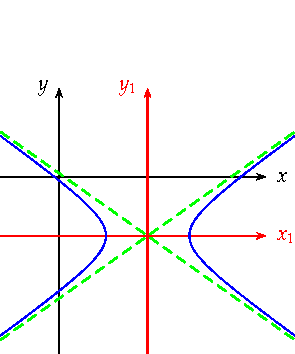
\includegraphics{hiperbole-eixos-tranladados.pdf}
        % \psset{unit=0.5cm}
        % \psset{ticksize=0pt}
        % \begin{pspicture*}(-2,-6)(8,6)
        %   \psaxes[labels=none]{->}(0,0)(-7,-7)(7,3)[$x$,0][$y$,-180]
        %   \psplot[algebraic,linestyle=dashed,linecolor=green]{-13}{13}{x/sqrt(2) - (3/sqrt(2) + 2)}
        %   \psplot[algebraic,linestyle=dashed,linecolor=green]{-13}{13}{-x/sqrt(2) + 3/sqrt(2) - 2}
        %   \psaxes[labels=none,linecolor=red]{->}(3,-2)(-7,-7)(7,3)[$\color{red} x_1$,0][$\color{red} y_1$,-180]
        %   \psplotImp[algebraic,linecolor=blue,stepFactor=0.1,linewidth=0.5pt](-4,-7)(10,7){(x-3)^2/2 - (y+2)^2  - 1}
        % \end{pspicture*}
      \end{figure}
    \end{solucao}
    \item $x^2 - y^2 + 2x - 6y - 8 = 0$
    \begin{solucao}
      Completando quadrados
      \begin{align*}
        &(x^2 - 2x + 1 - 1) - (y^2 + 6y + 9 - 9) - 8 = 0\\
        &(x - 1)^2 - (y + 3)^2 = 0\\
        &[(x - 1) - (y + 3)][(x - 1) + (y + 3)] = 0
      \end{align*}
      que representam as retas
      \begin{align*}
        r: x - y - 4 = 0\\
        s: x + y + 2 = 0
      \end{align*}
      que se interceptam no ponto $(1,-3)$.
    \end{solucao}
  \end{enumerate}
\end{exemplos}
% % subsection translacaoo_de_eixos (end)

\subsection{Rota\c{c}\~ao de eixos} % (fold)
\label{sub:rotacao_de_eixos}

Considere o sistema cartesiano com centro em $(0,0)$. Sejam $\vec{e_1} = (1,0)$ e $\vec{e_2} = (0,1)$. Para qualquer vetor $\vec{P} = (x,y)$ podemos escrever
\begin{align}\label{equacaoxy}
  \vec{P} = (x,y) = (x,0) + (0,y) = x(1,0) + y(0,1) = x\vec{e_1} + y\vec{e_2}.
\end{align}

\begin{figure}[!h]
  \centering
  \caption{Rota\c{c}\~ao de eixos: vetores $\vec{e_1}$ e $\vec{e_2}$}
  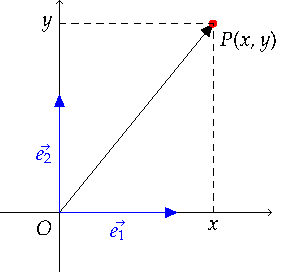
\includegraphics{rotacao-eixos-vetores-base.pdf}
  % \begin{tikzpicture}[scale=2]%vetor no plano
  %   \coordinate[label=below left:$O$] (A) at (0,0);
  %   \coordinate (W) at (1.3,1.6);
  %   %defini\c{c}\~ao das coordenadas dos eixos cartesianos
  %   \coordinate (F) at (-0.5,0);
  %   \coordinate (G) at (0,-0.5);
  %   \coordinate (X) at (1.8,0);
  %   \coordinate (Y) at (0,1.8);
  %   % Styles
  %   \tikzstyle{axes}=[]

  %   \begin{scope}[style=axes]%constr\'oi os eixos cartesianos
  %   \draw[->] (F) -- (X);
  %   \draw[->] (G) -- (Y);
  %   \end{scope}

  %   \draw[->,>=triangle 45] (A)--(W)
  %     node[below right]{$P(x, y)$};
  %     \draw [fill,color=red] (W) circle [radius=0.03];
  %   \draw[dashed,color=black] let \p1 = (W) in (\x1,0) -- (\x1,\y1)
  %     node[at start, below]{$x$};
  %   \draw[dashed,color=black] let \p1 = (W) in (0,\y1) -- (\x1,\y1)
  %     node[at start, left]{$y$};
  %   \draw[->,>=triangle 45,color=blue] (0,0) -- (1,0)
  %     node[midway, below]{$\vec{e_1}$};
  %     \draw[->,>=triangle 45,color=blue] (0,0) -- (0,1)
  %     node[midway, left]{$\vec{e_2}$};
  % \end{tikzpicture}
\end{figure}

Agora, efetuando-se uma rota\c{c}\~ao no sentido antihor\'ario nos eixos $x$ e $y$ de um \^angulo $\theta$, obtemos novos eixos coordenados $x_1$ e $y_1$. Tome vetores unit\'atios $\vec{u_1}$ e $\vec{u_1}$ nos eixos $x_1$ e $y_1$. Em rela\c{c}\~ao aos eixos originais podemos escrever
\begin{figure}[!h]
  \centering
  \caption{Rota\c{c}\~ao dos eixos por um \^angulo $\theta$}
  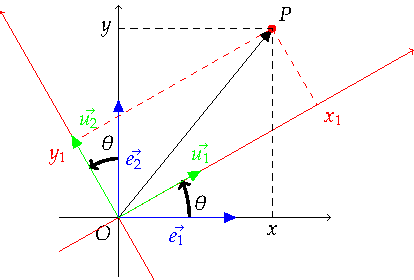
\includegraphics{rotacao-eixos.pdf}
  % \begin{tikzpicture}[scale=2]%vetor no plano
  %   \coordinate[label=below left:$O$] (A) at (0,0);
  %   \coordinate (W) at (1.3,1.6);
  %   %defini\c{c}\~ao das coordenadas dos eixos cartesianos
  %   \coordinate (F) at (-0.5,0);
  %   \coordinate (G) at (0,-0.5);
  %   \coordinate (X) at (1.8,0);
  %   \coordinate (Y) at (0,1.8);
  %   \coordinate (F1) at (-0.5,-0.285);%y=0,57x
  %   \coordinate (G1) at (0.3,-0.525);%y=-1,75x
  %   \coordinate (X1) at (2.5,1.42);%y=0,57x
  %   \coordinate (Y1) at (-1,1.75);%y=-1,75x
  %   % Styles
  %   \tikzstyle{axes}=[]

  %   \begin{scope}[style=axes]%constr\'oi os eixos cartesianos
  %     \draw[->] (F) -- (X);
  %     \draw[->] (G) -- (Y);
  %     \draw[->,color=red] (F1) -- (X1);
  %     \draw[->,color=red] (G1) -- (Y1);
  %   \end{scope}

  %   \draw [->,black,very thick](A) +(0:.6cm) arc (0:23:.8cm);
  %   \node at ($(A)+(10:7mm)$) {$\theta$};
  %   \draw [->,black,very thick](0,0.5) +(.4cm:0) arc (90:128:.4cm);
  %   \node at ($(0,0.5)+(125:1.6mm)$) {$\theta$};
  %   \draw[->,>=triangle 45] (A)--(W)
  %     node[at end,above right]{$P$};
  %   \draw [fill,color=red] (W) circle [radius=0.03];
  %   \draw[dashed,red] (W) -- ($(A)!(W)!(X1)$)
  %     node[at end,below right]{$x_1$};
  %   \draw[dashed,red] (W) -- ($(A)!(W)!(Y1)$)
  %     node[at end,below left]{$y_1$};
  %   \draw[dashed,color=black] let \p1 = (W) in (\x1,0) -- (\x1,\y1)
  %     node[at start, below]{$x$};
  %   \draw[dashed,color=black] let \p1 = (W) in (0,\y1) -- (\x1,\y1)
  %     node[at start, left]{$y$};
  %   \draw[->,>=triangle 45,color=blue] (0,0) -- (1,0)
  %     node[midway, below]{$\vec{e_1}$};
  %     \draw[->,>=triangle 45,color=blue] (0,0) -- (0,1)
  %     node[midway, right]{$\vec{e_2}$};
  %   \draw[->,>=triangle 45,color=green] (0,0) -- (0.7,0.399)%y=0,57x
  %     node[at end, above]{$\vec{u_1}$};
  %     \draw[->,>=triangle 45,color=green] (0,0) -- (-0.399,0.699)%y=-1,75x
  %     node[at end, above right]{$\vec{u_2}$};
  % \end{tikzpicture}
\end{figure}
\begin{align*}
  &\vec{u_1} = (\cos\theta,\sin\theta) = \cos\theta\vec{e_1} + \sin\theta\vec{e_2}\\
  &\vec{u_2} = (-\sin\theta,\cos\theta) = -\sin\theta\vec{e_1} + \cos\theta\vec{e_2}.
\end{align*}
Mas, os vetores $\vec{u_1}$ e $\vec{u_2}$ s\~ao unit\'arios e ortogonais, assim podemos escrever o vetor $\vec{P}$ como combina\c{c}\~ao de escalares nos eixos rotacionados, isto \'e,
\begin{equation}\label{equacaox1y1}
  \vec{P} = x_1\vec{u_1} + y_1\vec{u_2}.
\end{equation}

Da{\'\i} de \eqref{equacaoxy} e \eqref{equacaox1y1} obtemos
\[
  x\vec{e_1} + y\vec{e_2} = x_1\vec{u_1} + y_1\vec{u_2}
\]
e substituindo $\vec{u_1}$ e $\vec{u_2}$
\[
  x\vec{e_1} + y\vec{e_2} = (x_1\cos\theta - y_1\sin\theta)\vec{e_1} + (x_1\sin\theta + y_1\cos\theta)\vec{e_2}.
\]
Logo
\begin{align}
  &x = x_1\cos\theta - y_1\sin\theta\label{rotacaoX}\\
  &y = x_1\sin\theta + y_1\cos\theta\label{rotacaoY}
\end{align}
e ent\~ao isolando $x_1$ e $y_1$
\begin{align*}
  &x_1 = x\cos\theta + y\sin\theta\\
  &y_1 = -x\sin\theta + y\cos\theta.
\end{align*}
% Portanto para eliminar o termo $xy$ da equa\c{c}\~ao $g(x,y) = 0$, substitu{\'\i}mos \eqref{rotacaoX} e \eqref{rotacaoY} em $g(x,y) = 0$ e determinanos o \^angulo $\theta$ que elimina o termo $xy$.

\begin{exemplos}
  Seja $P$ o ponto $P(6,4)$. Efetuando-se uma rota\c{c}\~ao de um \^angulo de $\theta = \pi/3$ radianos nos eixos, as coordenadas de $P$ em rela\c{c}\~ao aos novos eixos s\~ao
    \begin{align*}
      x_1 = 6\cos(\pi/3) + 4\sin(\pi/3) = 3 + 2\sqrt{3}\\
      y_1 = -6\sin(\pi/3) + 4\cos(\pi/3) = 2 - 3\sqrt{3}.
    \end{align*}
    Da{\'\i} no novo sistema $P(3 + 2\sqrt{3}, 2 - 3\sqrt{3})$.
\end{exemplos}

% \begin{exemplos}
%   Identifique as c\^onicas:
%   \begin{enumerate}
%     \item $3x^2 + 3y^2 - 10xy + 12\sqrt{2}x - 4\sqrt{2}y + 32 = 0$
%     \begin{solucao}
%       Fazendo as mudan\c{c}as
%       \begin{align}
%         x = x_1\cos\theta - y_1\sin\theta\\
%         x = x_1\sin\theta + y_1\cos\theta
%       \end{align}
%       temos
%       \begin{align*}
%         &3(x_1\cos\theta - y_1\sin\theta)^2 + 3(x_1\sin\theta + y_1\cos\theta)^2\\ &- 10(x_1\cos\theta - y_1\sin\theta)(x_1\sin\theta + y_1\cos\theta)\\ & + 12\sqrt{2}(x_1\cos\theta - y_1\sin\theta) - 4\sqrt{2}(x_1\sin\theta + y_1\cos\theta)\\ &= (3\cos^2\theta + 3\sin^2\theta - 10\sin\theta\cos\theta)x_1^2 \\ &+ (3\sin^2\theta + 3\cos^2\theta + 10\sin\theta\cos\theta)y_1^2 \\ &+ (6\sin\theta\cos\theta - 10\cos^2\theta + 10\sin^2\theta - 6\sin\theta\cos\theta)x_1y_1 \\ &+ (12\sqrt{2}\cos\theta - 4\sqrt{2}\sin\theta)x_1 + (-12\sqrt{2}\sin\theta - 4\sqrt{2}\cos\theta)y_1 + 32 = 0.
%       \end{align*}
%       Assim $\theta$ deve ser tal que
%       \[
%         -10\cos^2\theta + 10\sin^2\theta = 0,
%       \]
%       isto \'e, $\theta = \pi/4$. Substituindo esse valor de $\theta$ na equa\c{c}\~ao anterior e simplificando obtemos
%       \[
%         x_1^2 - 4y_1^2 - 4x_1 + 8y_1 - 16 = 0.
%       \]
%       Nessa nova equa\c{c}\~ao podemos completar quadrados
%       \begin{align*}
%         &(x_1^2 - 4x_1 + 4) - 4 - 4(y_1^2 - 2y_1 + 1 - 1) - 16 = 0\\
%         &(x_1 - 2)^2 - 4(y_1 - 1)^2 = 16.
%       \end{align*}
%       Fazendo
%       \begin{align*}
%         x_2 = x_1 - 2\\
%         y_2 = y_1 - 1
%       \end{align*}
%       encontramos
%       \[
%         \dfrac{x_2^2}{16} - \dfrac{y_2^2}{4} = 1
%       \]
%       que \'e uma hip\'erbole de v\'ertices no eixo $x_2$.
%       \begin{figure}[!h]
%         \centering
%         \caption{Hip\'erbole $3x^2 +3y^2 - 10xy + 12\sqrt{2}x - 4\sqrt{2}y + 32 = 0$}
%         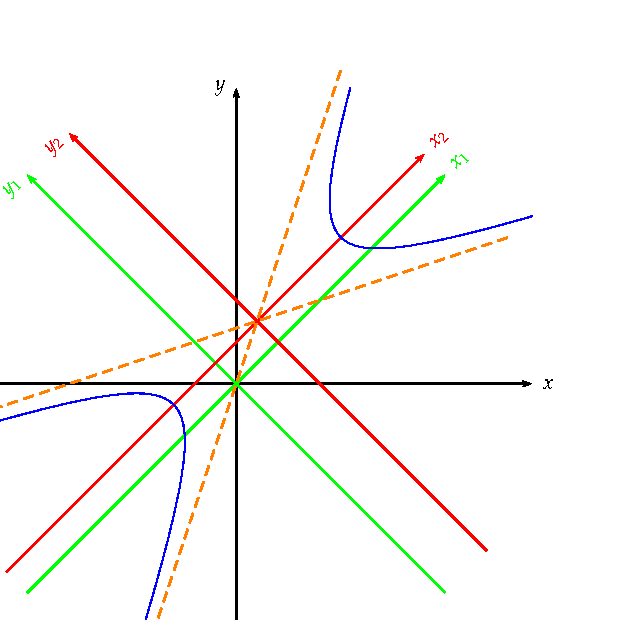
\includegraphics{hiperbole-rotacionada-transladada.pdf}
%       \end{figure}
%     \end{solucao}
%     \item $52x^2 - 72xy + 73y^2 - 400 = 0$
%     \begin{solucao}
%       Fazendo as mudan\c{c}as
%       \begin{align}
%         x = x_1\cos\theta - y_1\sin\theta\\
%         x = x_1\sin\theta + y_1\cos\theta
%       \end{align}
%       temos
%       \begin{align}\label{conicaelipse}
%         &52(x_1\cos\theta - y_1\sin\theta)^2 + 73(x_1\sin\theta + y_1\cos\theta)^2\nonumber \\ &- 72(x_1\cos\theta - y_1\sin\theta)(x_1\sin\theta + y_1\cos\theta) - 400 = 0\nonumber\\ &(52\cos^2\theta - 72\sin\theta\cos\theta + 73\sin^2\theta)x_1^2 + (52\sin^2\theta + 72\sin\theta\cos\theta + 73\cos^2\theta)y_1^2 \nonumber\\&+ (-104\sin\theta\cos\theta + 72\sin^2\theta - 72\cos^2\theta + 146\sin\theta\cos\theta)x_1y_1 - 400 = 0
%       \end{align}
%       Assim devemos ter
%       \begin{align*}
%         &-104\sin\theta\cos\theta + 72\sin^2\theta - 72\cos^2\theta + 146\sin\theta\cos\theta = 0\\
%         &42\sin\theta\cos\theta + 72(\sin^2\theta - \cos^2\theta) = 0\\
%         &21\sin(2\theta) - 72\cos(2\theta) = 0\\
%         &\tan(2\theta) = \dfrac{24}{7}.
%       \end{align*}
%       Agora
%       \[
%         \cos(2\theta) = \dfrac{1}{\sqrt{1 + \tan^2(2\theta)}}
%       \]
%       e usando as equa\c{c}\~oes $\cos^2\theta = (1/2)(1 + \cos(2\theta))$ e $\sin^2\theta = (1/2)(1 - \cos(2\theta))$ obtemos
%       \[
%         \cos\theta = \dfrac{4}{5} \quad \mbox{e}\quad \sin\theta = \dfrac{3}{5}.
%       \]
%       Substituindo na equa\c{c}\~ao \eqref{conicaelipse} obtemos
%       \begin{align*}
%         &\left(52\dfrac{16}{25} - 72\dfrac{12}{25} + 73\dfrac{9}{25}\right)x_1^2 + \left(52\dfrac{9}{25} + 72\dfrac{12}{25} + 73\dfrac{16}{25}\right)y_1^2 - 400 = 0\\
%         &25x_1^2 + 100y_1^2 = 400\\
%         &\dfrac{x_1^2}{16} + \dfrac{y_1^2}{4} = 1
%       \end{align*}
%       que representa uma elipse com focos no eixo $x_1$.
%       \begin{figure}[!h]
%         \centering
%         \caption{Elipse $52x^2 - 72xy + 73y^2 - 400 = 0$}
%         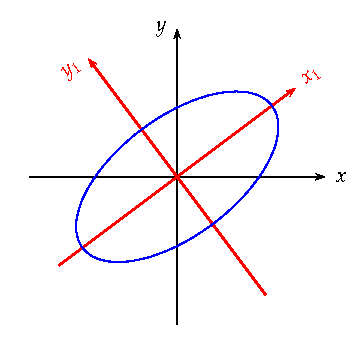
\includegraphics{elipse-rotacionada.pdf}
%       \end{figure}
%     \end{solucao}
%     \item $x^2 - 2xy + y^2 - 2x - 2y + 1 = 0$
%     \begin{solucao}
%       Fazendo as mudan\c{c}as
%       \begin{align}
%         x = x_1\cos\theta - y_1\sin\theta\\
%         x = x_1\sin\theta + y_1\cos\theta
%       \end{align}
%       temos
%       \begin{align}\label{conicaparabola}
%         &(x_1\cos\theta - y_1\sin\theta)^2 - 2(x_1\cos\theta - y_1\sin\theta)(x_1\sin\theta + y_1\cos\theta)\nonumber \\&+ (x_1\sin\theta + y_1\cos\theta)^2 - 2(x_1\cos\theta - y_1\sin\theta) - 2(x_1\sin\theta + y_1\cos\theta) + 1 = 0\nonumber\\
%         &(\cos^2\theta - 2\sin\theta\cos\theta + \sin^2\theta)x_1^2 + (\sin^2\theta + 2\sin\theta\cos\theta + \cos^2\theta)y_1^2\nonumber\\ &+ (-2\sin\theta\cos\theta - 2\cos^2\theta + 2\sin^2\theta + 2\sin\theta\cos\theta)x_1y_1\nonumber\\ &+ (-2\cos\theta - 2\sin\theta)x_1 + (2\sin\theta - 2\cos\theta)y_1 + 1 = 0.
%       \end{align}
%       Assim devemos ter
%       \[
%         -2\cos^2\theta + 2\sin^2\theta = 0,
%       \]
%       isto \'e, $\theta = \pi/4$. Substituindo em \eqref{conicaparabola} obtemos a equa\c{c}\~ao
%       \[
%         y_1^2 = \sqrt{2}\left(x_1 - \dfrac{1}{2\sqrt{2}}\right).
%       \]
%       Fazendo
%       \begin{align*}
%         x_1 - \dfrac{1}{2\sqrt{2}} = x_2\\
%         y_1 = y_2
%       \end{align*}
%       encontramos
%       \[
%         y_2^2 = \sqrt{2}x_2
%       \]
%       que representa uma par\'abola com foco no eixo $x_2$ e reta diretriz $x_2 = -\sqrt{2}/4$.
%       \begin{figure}[!h]
%         \centering
%         \caption{Par\'abola $x^2 - 2xy + y^2 - 2x - 2y + 1 = 0$}
%         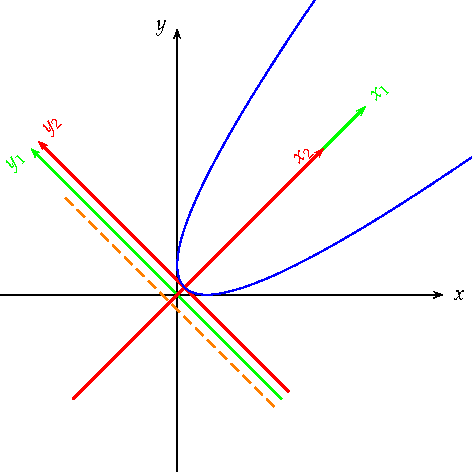
\includegraphics{parabola-rotacionada-transladada.pdf}
%       \end{figure}
%     \end{solucao}
%   \end{enumerate}
% \end{exemplos}

% subsection rotacao_de_eixos (end)

% \section{Rota\c{c}\~oes de Eixos: m\'etodo matricial} % (fold)
% \label{sec:rotacoes_de_eixos_metodo_matricial}

Considere uma c\^onica de equa\c{c}\~ao
\begin{equation}\label{equacao_geral_conica}
  ax^2 + bxy + cx^2 + dx + ey + f = 0.
\end{equation}

Queremos remover o termo $xy$ da equa\c{c}\~ao \eqref{equacao_geral_conica} para ent\~ao usar uma transla\c{c}\~ao de eixos, se necess\'ario, e com isso identicar a c\^onica definida por tal equa\c{c}\~ao. Para isso vamos tentar encontrar um \^angulo $\theta$ tal que a equa\c{c}\~ao \eqref{equacao_geral_conica} possa ser transformada numa equa\c{c}\~ao da forma
\begin{equation}\label{equacao_rotacionada_conica}
  a'x_1^2 + c'y_1^2 + d'x_1 + e'y_1 + f' = 0.
\end{equation}

Inicialmente observe que a \eqref{equacao_geral_conica} pode ser escrita na forma
\begin{equation}\label{equacao_matricial_conica}
  X^tAX + KX + F = [0]
\end{equation}
onde
\[
  A = \begin{bmatrix}
    a & b/2\\
    b/2 & c
  \end{bmatrix}
, \quad K = \begin{bmatrix}
  d & e
\end{bmatrix}, \quad X = \begin{bmatrix}
  x\\
  y
\end{bmatrix}\quad\mbox{e}\quad F = [f]
\]
e $t$ denota a matriz transposta. Queremos ent\~ao encontrar um \^angulo $\theta$ tal que a substitui\c{c}\~ao
\begin{equation}\label{substituicao_rotacao_eixos}
  X = \begin{bmatrix}
    \cos\theta & -\sin\theta\\
    \sin\theta & \cos\theta
  \end{bmatrix}\begin{bmatrix}
    x_1\\y_1
  \end{bmatrix}
\end{equation}
transforma a equa\c{c}\~ao \eqref{equacao_geral_conica} na equa\c{c}\~ao \eqref{equacao_rotacionada_conica}.

Sejam
\[
  R_\theta = \begin{bmatrix}
    \cos\theta & -\sin\theta\\
    \sin\theta & \cos\theta
  \end{bmatrix}
\]
que \'e chamada de \textbf{matriz de rota\c{c}\~ao} e
\[
  X_1 = \begin{bmatrix}x_1\\y_1\end{bmatrix}.
\]
Note que
\[
  R_\theta R_\theta^t = \begin{bmatrix}
    \cos\theta & -\sin\theta\\
    \sin\theta & \cos\theta
  \end{bmatrix}\begin{bmatrix}
    \cos\theta & \sin\theta\\
    -\sin\theta & \cos\theta
  \end{bmatrix} = \begin{bmatrix}
    1 & 0\\
    0 & 1
  \end{bmatrix} = R_\theta^t R_\theta, 
\]
ou seja, $(R_\theta^t)^{-1} = R_\theta$.

Agora, substituindo \eqref{substituicao_rotacao_eixos} em \eqref{equacao_geral_conica} obtemos
\begin{align*}
  (R_\theta X_1)^t A (R_\theta X_1) + KR_\theta X_1 + F = [0]\\
  X_1^t(R_\theta^t A R_\theta)X_1 + (KR_\theta)X_1 + F = [0].
\end{align*}
Note que
\begin{align*}
  R_\theta^t A R_\theta = \begin{bmatrix}
    a' & b'/2\\
    b'/2 & c'
  \end{bmatrix} = B\\
  KR_\theta = \begin{bmatrix}
    d'& e'
  \end{bmatrix} = K'.
\end{align*}

Mas $I_2 = R_\theta^t R_\theta$ e da{\'\i} podemos escrever
\begin{align*}
  B - \lambda I_2 = R_\theta^t A R_\theta - \lambda I_2 = R_\theta^t A R_\theta - R_\theta^t (\lambda I_2) R_\theta = R_\theta^t (A - \lambda I_2)R_\theta
\end{align*}
para todo $\lambda \in \real$. Com isso
\begin{align*}
  \det(B - \lambda I_2) = \det[R_\theta^t(A - \lambda I_2)R_\theta] = \det(R_\theta^t)\det(A - \lambda I_2)\det(R_\theta) = \det(A - \lambda I_2).
\end{align*}

Assim escolhendo $\theta$ tal que $b' = 0$, o que \'e sempre poss{\'\i}vel fazer, obtemos
\begin{align*}
  \det(A - \lambda I_2) = \det(B - \lambda I_2) = \det \begin{bmatrix}
    a' - \lambda & 0\\
    0 & c' - \lambda
  \end{bmatrix} = (\lambda - a')(\lambda - c').
\end{align*}

Logo os coeficientes $a'$ e $c'$ s\~ao ra{\'\i}zes da equa\c{c}\~ao de segundo grau
\begin{equation}
  p(\lambda) = \det(A - \lambda I_2) = \det \begin{bmatrix}
    a - \lambda & b/2\\
    b/2 & c - \lambda
  \end{bmatrix}.
\end{equation}

Agora para determinar o \^angulo $\theta$ partimos de
\[
  B = R_\theta^t A R_\theta
\]
e multiplicamos \`a esquerda por $R_\theta$ obtendo
\[
  R_\theta B = AR_\theta.
\]
Da{\'\i}
\begin{align*}
  AR_\theta = A \begin{bmatrix}
    \cos\theta & -\sin\theta\\
    \sin\theta & \cos\theta
  \end{bmatrix} = \begin{bmatrix}
    A \begin{bmatrix}
      \cos\theta \\ \sin\theta
    \end{bmatrix} & A \begin{bmatrix}
      -\sin\theta\\ \cos\theta
    \end{bmatrix}
  \end{bmatrix}
\end{align*}
e
\begin{align*}
  R_\theta B = \begin{bmatrix}
    \cos\theta & -\sin\theta\\
    \sin\theta & \cos\theta
  \end{bmatrix} \begin{bmatrix}
    a' & 0\\
    0 & c'
  \end{bmatrix} = \begin{bmatrix}
    a' \begin{bmatrix}
      \cos\theta \\ \sin\theta
    \end{bmatrix} & c' \begin{bmatrix}
      -\sin\theta\\ \cos\theta
    \end{bmatrix}
  \end{bmatrix}.
\end{align*}

Como $R_\theta B = AR_\theta$ ent\~ao das duas \'ultimas equa\c{c}\~ao vemos que se tomarmos
\[
  U_1 = \begin{bmatrix}
    \cos\theta\\
    \sin\theta
  \end{bmatrix} = (\cos\theta, \sin\theta)
\]
devemos ter
\[
  AU_1 = a'U_1,
\]
isto \'e,
\begin{align*}
  AU_1 = a'I_2 U_1\\
  AU_1 - a'I_2 U_1 = [0]\\
  (A - a'I_2)U_1 = [0].
\end{align*}
Assim $U_1$ \'e uma solu\c{c}\~ao de norma 1 do sistema linear
\[
  (A - a'I_2)X = [0].
\]
A solu\c{c}\~ao $U_2$ \'e obtida de $U_1$ trocando a posi\c{c}\~ao das componentes de $U_1$ e depois o sinal da primeira posi\c{c}\~ao.

Portanto a rota\c{c}\~ao que elemina o termo $xy$ \'e dada por $R_\theta = [U_1\ U_2]$. Assim temos o seguinte teorema:

\begin{teorema}
  Considere a equa\c{c}\~ao
  \[
      ax^2 + bxy + cy^2 + dx + ey + f = 0
  \]
  com $a$, $b$, $c$, $d$, $e$, $f \in \real$, sendo $a$, $b$ e $c$ n\~ao necessariamente nulos. Ent\~ao mediante uma rota\c{c}\~ao da forma
  \[
    X = R_\theta X_1
  \]
  onde
  \[
    X = \begin{bmatrix}
      x\\y
    \end{bmatrix}, \quad
    R_\theta = \begin{bmatrix}
    \cos\theta & -\sin\theta\\
    \sin\theta & \cos\theta
  \end{bmatrix}, \quad\mbox{e}\quad
  X_1 = \begin{bmatrix}
    x_1\\y_1
  \end{bmatrix}
  \]
  a equa\c{c}\~ao da c\^onica acima pode ser transformada em
  \[
    a'x_1^2 + c'y_1^2 + d'x_1 + e'y_1 + f = 0
  \]
  em que $a'$, $c'$ s\~ao ra{\'\i}zes de
  \[
    p(\lambda) = \det(A - \lambda I_2) = \det \begin{bmatrix}
      a - \lambda & b/2\\
      b/2 & c - \lambda
    \end{bmatrix}.
  \]

  Mais ainda,
  \[
    U_1 = \begin{bmatrix}
      \cos\theta\\ \sin\theta
    \end{bmatrix}
  \]
  \'e uma solu\c{c}\~ao de norma 1 do sistema linear
  \[
    \begin{bmatrix}
      a - a' & b/2\\
      b/2 & c - a'
    \end{bmatrix} \begin{bmatrix}
      x\\y
    \end{bmatrix} = \begin{bmatrix}
      0\\0
    \end{bmatrix}.
  \]
\end{teorema}

\begin{exemplos}
  Identifique as c\^onicas:
  \begin{enumerate}
    \item $52x^2 - 72xy + 73y^2 - 400 = 0$
    \begin{solucao}
      Inicialmente podemos escrever tal equa\c{c}\~ao na forma
      \[
        X^t A X + KX - 400 = 0
      \]
      onde
      \[
        X = \begin{bmatrix}
          x\\y
        \end{bmatrix}, \quad A = \begin{bmatrix}
          52 & -36\\
          -36 & 73
        \end{bmatrix},\quad K = \begin{bmatrix}
          0 & 0
        \end{bmatrix}.
      \]
      Fazendo a mudan\c{c}a $X = R_\theta X_1$ onde
      \[
        X_1 = \begin{bmatrix}
          x_1 \\y_1
        \end{bmatrix} \quad\mbox{e}\quad R_\theta = \begin{bmatrix}
          \cos\theta & -\sin\theta\\
          \sin\theta & \cos\theta
        \end{bmatrix}
      \]
      removeremos o termo $xy$. Para isso precisamos encontrar as ra{\'\i}zes de
      \begin{align*}
        p(\lambda) &= \det (A - \lambda I_2) = \det \begin{bmatrix}
          52 - \lambda & -36\\
          -36 & 73 - \lambda
        \end{bmatrix} \\ &= (52 - \lambda)(73 - \lambda) - 36^2 \\ &= \lambda^2 - 125\lambda + 2500.
      \end{align*}
      Suas ra{\'\i}zes s\~ao $\lambda_1 = 25$ e $\lambda_2 = 100$. Tomando $a' = 25$ e $c' = 100$ precisamos resolver o sistema
      \begin{align*}
        (A - 25I_2)X = \begin{bmatrix}
          0\\0
        \end{bmatrix}\\
        \begin{bmatrix}
          27 & -36\\
          -36 & 48
        \end{bmatrix} \begin{bmatrix}
          x \\y
        \end{bmatrix} = \begin{bmatrix}
          0 \\0
        \end{bmatrix}
      \end{align*}
      para encontrar a matrix de rota\c{c}\~ao. A solu\c{c}\~ao deste sistema \'e $x = (4/3)y$ e para determinar a matriz precisamos escolher solu\c{c}\~oes de norma 1. Assim podemos tomar, por exemplo,
      \begin{align*}
        U_1 = (\cos\theta, \sin\theta) = (4/5, 3/5)\\
        U_2 = (-\sin\theta, \cos\theta) = (-3/5, 4/5).
      \end{align*}
      Da{\'\i} o \^angulo de rota\c{c}\~ao \'e $\theta = \arccos(4/5)$, a matriz de rota\c{c}\~ao \'e
      \[
        R_\theta = \begin{bmatrix}
          4/5 & -3/5\\
          3/5 & 4/5
        \end{bmatrix}
      \]
      e
      \[
        B = \begin{bmatrix}
          25 & 0\\
          0 & 100
        \end{bmatrix}.
      \]
      Com isso a equa\c{c}\~ao original torna-se
      \begin{align*}
        25x_1^2 + 100y_1^2 = 400\\
        \dfrac{x_1^2}{16} + \dfrac{y_1^2}{4} = 1
      \end{align*}
      que \'e uma elipse com focos no eixo $x_1$.
      \begin{figure}[!h]
        \centering
        \caption{Elipse $52x^2 - 72xy + 73y^2 - 400 = 0$}
        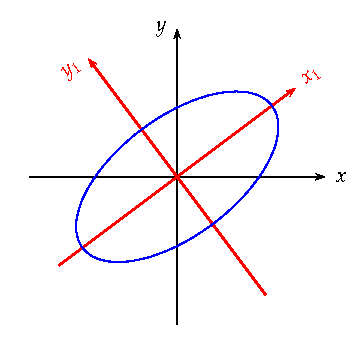
\includegraphics{elipse-rotacionada.pdf}
      \end{figure}
    \end{solucao}

    \item $x^2 - 2xy + y^2 - 2x - 2y + 1 = 0$
    \begin{solucao}
      Inicialmente podemos escrever tal equa\c{c}\~ao na forma
      \[
        X^t A X + KX + 1 = 0
      \]
      onde
      \[
        X = \begin{bmatrix}
          x\\y
        \end{bmatrix}, \quad A = \begin{bmatrix}
          1 & -1\\
          -1 & 1
        \end{bmatrix},\quad K = \begin{bmatrix}
          -2 & -2
        \end{bmatrix}.
      \]
      Fazendo a mudan\c{c}a $X = R_\theta X_1$ onde
      \[
        X_1 = \begin{bmatrix}
          x_1 \\y_1
        \end{bmatrix} \quad\mbox{e}\quad R_\theta = \begin{bmatrix}
          \cos\theta & -\sin\theta\\
          \sin\theta & \cos\theta
        \end{bmatrix}
      \]
      removeremos o termo $xy$. Para isso precisamos encontrar as ra{\'\i}zes de
      \begin{align*}
        p(\lambda) &= \det (A - \lambda I_2) = \det \begin{bmatrix}
          1 - \lambda & -1\\
          -1 & 1 - \lambda
        \end{bmatrix} \\ &= (1 - \lambda)^2 - 1 = \lambda^2 - 2\lambda.
      \end{align*}
      Suas ra{\'\i}zes s\~ao $\lambda_1 = 0$ e $\lambda_2 = 2$. Tomando $a' = 0$ e $c' = 2$ precisamos resolver o sistema
      \begin{align*}
        (A - 0I_2)X = \begin{bmatrix}
          0\\0
        \end{bmatrix}\\
        \begin{bmatrix}
          1 & -1\\
          -1 & 1
        \end{bmatrix} \begin{bmatrix}
          x \\y
        \end{bmatrix} = \begin{bmatrix}
          0 \\0
        \end{bmatrix}
      \end{align*}
      para encontrar a matrix de rota\c{c}\~ao. A solu\c{c}\~ao deste sistema \'e $x = y$ e para determinar a matriz precisamos escolher solu\c{c}\~oes de norma 1. Assim podemos tomar, por exemplo,
      \begin{align*}
        U_1 = (\cos\theta, \sin\theta) = (1/\sqrt{2}, 1/\sqrt{2})\\
        U_2 = (-\sin\theta, \cos\theta) = (-1/\sqrt{2}, 1/\sqrt{2}).
      \end{align*}
      Da{\'\i} o \^angulo de rota\c{c}\~ao \'e $\theta = \arccos(1/\sqrt{2}) = \pi/4$, a matriz de rota\c{c}\~ao \'e
      \[
        R_\theta = \begin{bmatrix}
          1/\sqrt{2} & -1/\sqrt{2}\\
          1/\sqrt{2} & 1/\sqrt{2}
        \end{bmatrix}
      \]
      e
      \[
        B = \begin{bmatrix}
          0 & 0\\
          0 & 2
        \end{bmatrix}.
      \]
      Com isso a equa\c{c}\~ao original torna-se
      \begin{align*}
        2y_1^2 - 4\sqrt{2}x_1 + 1 = 0\\
        y_1^2 = \sqrt{2}\left(x_1 - \dfrac{1}{2\sqrt{2}}\right).
      \end{align*}
      Fazendo a mudan\c{c}a
      \begin{align*}
        x_2 = x_1 - \dfrac{1}{2\sqrt{2}}\\
        y_2 = y_1
      \end{align*}
      obtemos a equa\c{c}\~ao
      \[
        y_2^2 = \sqrt{2}x_2
      \]
      que \'e uma par\'abola com foco no eixo $x_2$ e reta diretriz $r: x_2 = -\sqrt{2}/4$.
      \begin{figure}[!h]
        \centering
        \caption{Par\'abola $x^2 - 2xy + y^2 - 2x - 2y + 1 = 0$}
        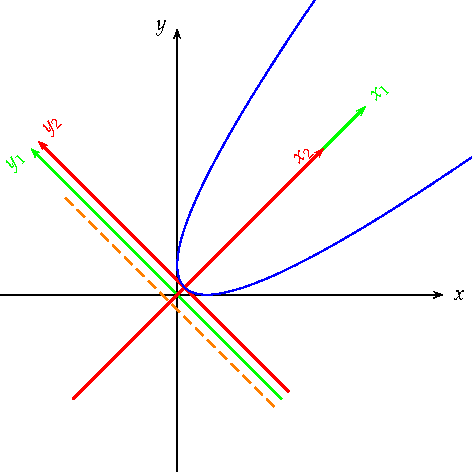
\includegraphics{parabola-rotacionada-transladada.pdf}
      \end{figure}
    \end{solucao}

    \item $3x^2 - 10xy + 3y^2 - 12\sqrt{2}x - 4\sqrt{2}y + 32 = 0$
    \begin{solucao}
      Inicialmente podemos escrever tal equa\c{c}\~ao na forma
      \[
        X^t A X + KX + 1 = 0
      \]
      onde
      \[
        X = \begin{bmatrix}
          x\\y
        \end{bmatrix}, \quad A = \begin{bmatrix}
          3 & -5\\
          -5 & 3
        \end{bmatrix},\quad K = \begin{bmatrix}
          12\sqrt{2} & -4\sqrt{2}
        \end{bmatrix}.
      \]
      Fazendo a mudan\c{c}a $X = R_\theta X_1$ onde
      \[
        X_1 = \begin{bmatrix}
          x_1 \\y_1
        \end{bmatrix} \quad\mbox{e}\quad R_\theta = \begin{bmatrix}
          \cos\theta & -\sin\theta\\
          \sin\theta & \cos\theta
        \end{bmatrix}
      \]
      removeremos o termo $xy$. Para isso precisamos encontrar as ra{\'\i}zes de
      \begin{align*}
        p(\lambda) &= \det (A - \lambda I_2) = \det \begin{bmatrix}
          3 - \lambda & -5\\
          -5 & 3 - \lambda
        \end{bmatrix}\\ &= (3 - \lambda)^2 - 25\\ &= \lambda^2 - 6\lambda - 16.
      \end{align*}
      Suas ra{\'\i}zes s\~ao $\lambda_1 = -2$ e $\lambda_2 = 8$. Tomando $a' = -2$ e $c' = 8$ precisamos resolver o sistema
      \begin{align*}
        (A + 2I_2)X = \begin{bmatrix}
          0\\0
        \end{bmatrix}\\
        \begin{bmatrix}
          5 & -5\\
          -5 & 5
        \end{bmatrix} \begin{bmatrix}
          x \\y
        \end{bmatrix} = \begin{bmatrix}
          0 \\0
        \end{bmatrix}
      \end{align*}
      para encontrar a matrix de rota\c{c}\~ao. A solu\c{c}\~ao deste sistema \'e $x = y$ e para determinar a matriz precisamos escolher solu\c{c}\~oes de norma 1. Assim podemos tomar, por exemplo,
      \begin{align*}
        U_1 = (\cos\theta, \sin\theta) = (1/\sqrt{2}, 1/\sqrt{2})\\
        U_2 = (-\sin\theta, \cos\theta) = (-1/\sqrt{2}, 1/\sqrt{2}).
      \end{align*}
      Da{\'\i} o \^angulo de rota\c{c}\~ao \'e $\theta = \arccos(1/\sqrt{2}) = \pi/4$, a matriz de rota\c{c}\~ao \'e
      \[
        R_\theta = \begin{bmatrix}
          1/\sqrt{2} & -1/\sqrt{2}\\
          1/\sqrt{2} & 1/\sqrt{2}
        \end{bmatrix}
      \]
      e
      \[
        B = \begin{bmatrix}
          -2 & 0\\
          0 & 8
        \end{bmatrix}.
      \]
      Com isso a equa\c{c}\~ao original torna-se
      \begin{align*}
        -2x_1^2 + 8y_1^2 + 8x_1 -16y_1 + 32 = 0\\
        x_1^2 - 4y_1^2 - 4x_1 + 8y_1 -16 = 0\\
        (x_1^2 - 4x_1 + 4) - 4 - 4(y_1^2 - 2y_1 + 1) + 4 - 16 = 0\\
        (x_1 - 2)^2 - 4(y_1 - 1)^2 = 16
      \end{align*}
      Fazendo a mudan\c{c}a
      \begin{align*}
        x_2 = x_1 - 2\\
        y_2 = y_1 - 1
      \end{align*}
      obtemos a equa\c{c}\~ao
      \[
        \dfrac{x_2^2}{16} - \dfrac{y_2^2}{4} = 1
      \]
      que \'e uma hip\'erbole com focos no eixo $x_2$.
      \begin{figure}[!h]
        \centering
        \caption{Hip\'erbole $3x^2 +3y^2 - 10xy + 12\sqrt{2}x - 4\sqrt{2}y + 32 = 0$}
        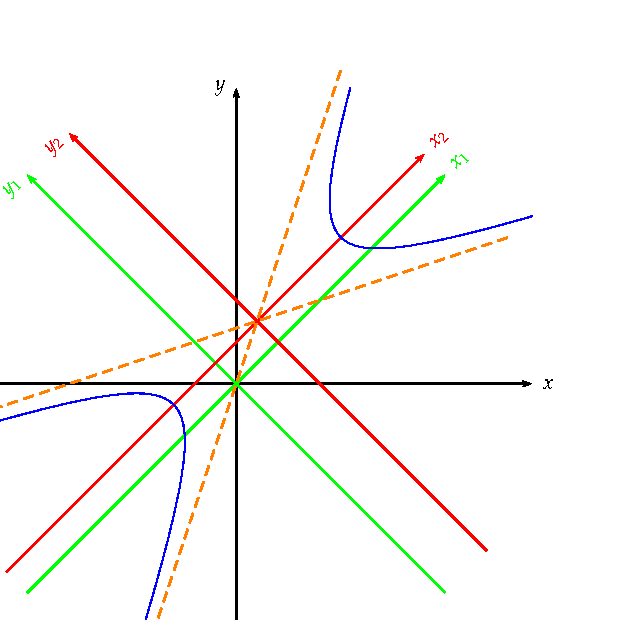
\includegraphics{hiperbole-rotacionada-transladada.pdf}
      \end{figure}
    \end{solucao}
  \end{enumerate}
\end{exemplos}

\begin{teorema}
  Seja $\mathcal{C}$ o conjunto dos pontos do plano que satisfazem a equa\c{c}\~ao
  \[
    ax^2 + bxy + cy^2 + dx + ey + f = 0,
  \]
  com $a$, $b$, $c$, $d$, $e$, $f \in \real$, sendo $a$, $b$ e $c$ n\~ao simultaneamente nulos. Sejam $a'$ e $c'$ ra{\'\i}zes de
  \[
    p(\lambda) = \det \begin{bmatrix}
      a - \lambda & b/2\\
      b/2 & c - \lambda
    \end{bmatrix}.
  \]
  \begin{enumerate}[label=({\roman*})]
    \item Temos $a'c' = ac - b^2/4$.
    \item Se $a'c' > 0$, ent\~ao $\mathcal{C}$ \'e uma elipse, um ponto ou o conjunto vazio.
    \item Se $a'c' < 0$, ent\~ao $\mathcal{C}$ \'e uma hip\'erbole ou um par de retas concorrentes.
    \item Se $a'c' = 0$, ent\~ao $\mathcal{C}$ \'e uma par\'abola, um par de retas paralelas, uma reta ou o conjunto vazio.
  \end{enumerate}
\end{teorema}
% section rotacoes_de_eixos_metodo_matricial (end)

% section rotacao_e_translacao_de_eixos (end)

% \section{Se\c{c}\~oes C\^onicas} % (fold)
% \label{sec:secoes_conicas}
% \missingfigure{Figuras de se\c{c}\~oes c\^onicas}
% section secoes_conicas (end)

% chapter circunferencias_e_conicas (end)
%!TEX program = xelatex
%!TEX root = geometria_analitica.tex
%%Usar makeindex -s indexstyle.ist arquivo.idx no terminal para gerar o {\'\i}ndice remissivo agrupado por inicial
%%Ap\'os executar pdflatex arquivo

\chapter{Vetores no Espa\c{c}o} % (fold)
\label{cha:vetores_no_espaco}

Fixemos um ponto $O$ no espa\c{c}o, que ser\'a denominado como \textbf{origem}. Tomemos tr\^es retas duas a duas perpendiculares entre si e concorrentes em $O$, que ser\~ao denominados \textbf{eixos coordenados} e ser\~ao denotados por $Ox$, $Oy$ e $Oz$.
\begin{figure}[!h]
  \centering
  \caption{Sistema de coordenadas tridimensionais}
  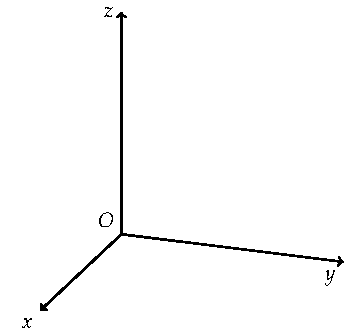
\includegraphics{eixos-coordenados-espaco.pdf}
  % \tdplotsetmaincoords{70}{110}
  % \begin{tikzpicture}[scale=2,tdplot_main_coords]
  %   \coordinate[label=above left:$O$] (A) at (0,0,0);
    
  %   %constr\'oi os eixos cartesianos
  %   \draw[thick,->,black] (0,0,0) -- (2,0,0) node[anchor=north east]{$x$};
  %   \draw[thick,->] (0,0,0) -- (0,2,0) node[anchor=north east]{$y$};
  %   \draw[thick,->] (0,0,0) -- (0,0,2) node[anchor=east]{$z$};
  %   \end{tikzpicture}
\end{figure}

Projetando um ponto $P$ do espa\c{c}o ortogonalmente sobre cada um dos eixos coordenados podemos representar os pontos do espa\c{c}o por ternas ordenadas $(a,b,c)$ de n\'umeros reais.

\begin{figure}[!h]
  \centering
  \caption{Coordenadas de um ponto no espa\c{c}o tridimensional}
  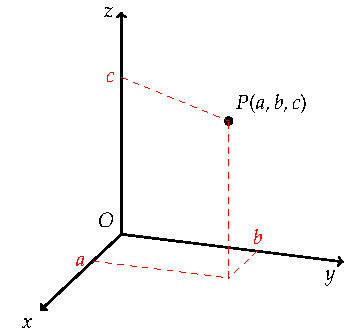
\includegraphics{coordenadas-ponto-espaco.pdf}
  % \tdplotsetmaincoords{70}{110}
  % \begin{tikzpicture}[scale=2,tdplot_main_coords]
  %   \coordinate[label=above left:$O$] (A) at (0,0,0);
    
  %   %constr\'oi os eixos cartesianos
  %   \draw[thick,->,black] (0,0,0) -- (2,0,0) node[anchor=north east]{$x$};
  %   \draw[thick,->] (0,0,0) -- (0,2,0) node[anchor=north east]{$y$};
  %   \draw[thick,->] (0,0,0) -- (0,0,2) node[anchor=east]{$z$};

  %   \tdplotsetcoord{P}{2}{45}{60}
  %   \filldraw (P) circle (1pt) node[above right]{$P(a, b, c)$};

  %   \draw[dashed, color=red] (Px) -- (Pxy) node[at start,left]{$a$};
  %   \draw[dashed, color=red] (Py) -- (Pxy)node[at start,above]{$b$};
  %   \draw[dashed, color=red] (Pz) -- (P)node[at start,left]{$c$};
  %   \draw[dashed, color=red] (Pxy) -- (P);
  %   \end{tikzpicture}
\end{figure}

Assim os pontos de $\real^3$ s\~ao descritos por
\[
  \real^3 = \{(a,b,c)\mid a,b,c \in \real\}.
\]

Sejam $P(x_1,y_1,z_1)$ e $Q(x_2,y_2,z_2)$ dois pontos de $\real^3$. Tra\c{c}ando por $P$ um segmento $PS$ paralelo ao segmento $P_0Q_0$, onde $P_0(x_1,y_1)$ e $Q_0(x_2,y_2)$, obtemos que
\[
  d(P,Q)^2 = d(P_0,Q_0)^2 + |SQ|^2.
\]
\begin{figure}
  \centering
  \caption{Dist\^ancia entre pontos em $\real^3$}
  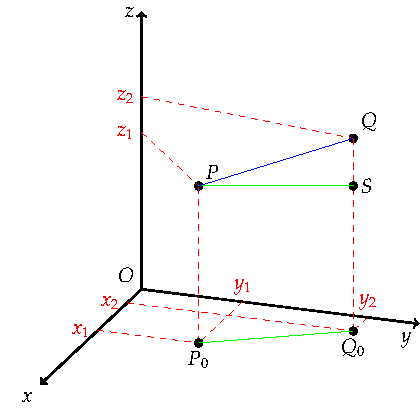
\includegraphics{distancia-pontos-espaco.pdf}
  % \tdplotsetmaincoords{70}{110}
  % \begin{tikzpicture}[scale=2,tdplot_main_coords]
  %   \coordinate[label=above left:$O$] (A) at (0,0,0);
    
  %   %constr\'oi os eixos cartesianos
  %   \draw[thick,->,black] (0,0,0) -- (2.5,0,0) node[anchor=north east]{$x$};
  %   \draw[thick,->] (0,0,0) -- (0,2.5,0) node[anchor=north east]{$y$};
  %   \draw[thick,->] (0,0,0) -- (0,0,2.5) node[anchor=east]{$z$};

  %   \tdplotsetcoord{P}{2}{45}{40}
  %   \filldraw (P) circle (1pt) node[above right]{$P$};
  %   \tdplotsetcoord{Q}{2.7}{50}{80}
  %   \filldraw (Q) circle (1pt) node[above right]{$Q$};

  %   \draw[dashed, color=red] (Px) -- (Pxy) node[at start,left]{$x_1$};
  %   \draw[dashed, color=red] (Py) -- (Pxy)node[at start,above]{$y_1$};
  %   \draw[dashed, color=red] (Pz) -- (P)node[at start,left]{$z_1$};
  %   \draw[dashed, color=red] (Pxy) -- (P);
  %   \draw[dashed, color=red] (Qx) -- (Qxy) node[at start,left]{$x_2$};
  %   \draw[dashed, color=red] (Qy) -- (Qxy)node[at start,above]{$y_2$};
  %   \draw[dashed, color=red] (Qz) -- (Q)node[at start,left]{$z_2$};
  %   \draw[dashed, color=red] (Qxy) -- (Q);

  %   \filldraw ($(Q)!(P)!(Qxy)$) circle (1pt)node[right]{$S$};
  %   \draw[color=green] ($(Q)!(P)!(Qxy)$) -- (P);
  %   \filldraw (Pxy) circle (1pt) node[below]{$P_0$};
  %   \filldraw (Qxy) circle (1pt) node[below]{$Q_0$};

  %   \draw[color=blue] (P) -- (Q);
  %   \draw[color=green] (Pxy) -- (Qxy);
  %   \end{tikzpicture}
\end{figure}

Agora, $|SQ| = |z_2 - z_1|$ e da{\'\i}
\[
  D(P,Q) = \sqrt{(x_1 - x_2)^2 + (y_1 - y_2)^2 + (z_1 - z_2)^2}.
\]

\begin{exemplos}
  A dist\^ancia entre os pontos $P(2,-1,1)$ e $Q(-3,4,2)$ \'e
  \[
    d(P,Q) = \sqrt{[2 - (-3)]^2 + (-1-4)^2 + (1-2)^2} = \sqrt{51}.
  \]
\end{exemplos}

Os vetores e as opera\c{c}\~oes com eles podem ser definidas utilizando-se dos eixos coordenados do espa\c{c}o. Para isso, um ponto $P$ do espa\c{c}o \'e representado em $\real^3$ por uma terna de coordenadas $P(x_1, y_1,z_1)$, onde $x_1$, $y_1$, $z_1 \in \real$.

Seja $\vec{u}$ um vetor no espa\c{c}o. Sabemos que $\vec{u}$ \'e um representante de uma certa classe de equipol\^encia dos segmentos orientados $(B,C)$. Para este segmento orientado $(B,C)$ podemos encontrar um ponto $A(x_1, y_1,z_1)$ tal que o segmento orientado $(O,A)$, onde $O(0,0,0)$, tem o mesmo comprimento, a mesma dire\c{c}\~ao e o mesmo sentido de $(B,C)$. Assim o vetor $\vec{u}$ pode ser representado pelo segmento orientado $(O,A)$. Portanto qualquer vetor em $\real^3$ pode ser representado como um segmento com origem no ponto $(0,0,0)$ e extremidade em um ponto $(x_1,y_1,z_1)$.


Assim escrevemos $\vec{u} = \vec{OP}$. Para simplificar a nota\c{c}\~ao vamos identificar o vetor $\vec{u} = \vec{OP}$ com as coordenadas de sua extremidade e da{\'\i} escrevemos
\[
  \vec{u} = (x_1,y_1,z_1).
\]
As coordenadas $(x_1,y_1,z_1)$ s\~ao chamadas de \textbf{componentes} do vetor $\vec{u}$. Com essa representa\c{c}\~ao, o vetor nulo $\vec{0}$ \'e escrito como
\[
  \vec{0} = (0,0,0).
\]

Desse modo, podemos reescrever a defini\c{c}\~ao de soma e produto por escalar da seguinte forma:
\begin{definicao}
  Sejam $\alpha \in \real$, $\vec{u} = (x_1, y_1,z_1)$ e $\vec{v} = (x_2, y_2,z_2)$. Ent\~ao:
  \begin{enumerate}
    \item $\vec{u} + \vec{v} = (x_1 + x_2, y_1 + y_2,z_1 + z_2)$;
    \item $\alpha \vec{u} = (\alpha x_1, \alpha y_1, \alpha z_1)$.
  \end{enumerate}
\end{definicao}

% \begin{center}
%   \begin{tikzpicture}[scale=2]%soma de vetores no plano
%     \coordinate (A) at (0,0);
%     \coordinate (V) at (0.5,1);
%     \coordinate (W) at (1,0.5);
%     \coordinate (B) at (0,1);
%     \coordinate (VW) at ($(V)+(W)$);
%     %defini\c{c}\~ao das coordenadas dos eixos cartesianos
%     \coordinate (F) at (-1,0);
%     \coordinate (G) at (0,-1);
%     \coordinate (X) at (2,0);
%     \coordinate (Y) at (0,2);
%     % Styles
%     \tikzstyle{axes}=[]

%     \begin{scope}[style=axes]%constr\'oi os eixos cartesianos
%     \draw[->] (F) -- (X) node[below] {$x$} coordinate(x axis);
%     \draw[->] (G) -- (Y) node[left] {$y$} coordinate(y axis);
%     \end{scope}

%     \draw[->,>=triangle 45,color=blue] (A)--(V)
%       node[above]{$\vec{u}$};
%     \draw[->,>=triangle 45,color=blue] (A)--(W)
%       node[below right]{$\vec{v}$};
%     \draw[->,>=triangle 45,color=red] (A)--(VW)
%       node[below right]{$\vec{u}+\vec{v}$};
%     \draw[dashed,>=triangle 45,color=blue] (V)--(VW);
%     \draw[dashed,>=triangle 45,color=blue] (W)--(VW);
%     \draw[dashed,color=black] let \p1 = (V) in (\x1,0) -- (\x1,\y1)
%       node[at start, below]{$x_1$};
%     \draw[dashed,color=black] let \p1 = (V) in (0,\y1) -- (\x1,\y1)
%       node[at start, left]{$y_1$};
%     \draw[dashed,color=black] let \p1 = (W) in (\x1,0) -- (\x1,\y1)
%       node[at start, below]{$x_2$};
%     \draw[dashed,color=black] let \p1 = (W) in (0,\y1) -- (\x1,\y1)
%       node[at start, left]{$y_2$};
%     \draw[dashed,color=black] let \p1 = (VW) in (\x1,0) -- (\x1,\y1)
%       node[at start, below]{$x_1 + x_2$};
%     \draw[dashed,color=black] let \p1 = (VW) in (0,\y1) -- (\x1,\y1)
%       node[at start, left]{$y_1 + y_2$};
%   \end{tikzpicture}

%   \begin{tikzpicture}[scale=2]%multiplica\c{c}\~ao por escalar no plano
%     \coordinate (A) at (0,0);
%     \coordinate (V) at (0.5,0.5);
%     \coordinate (W) at ($2*(V)$);
%     %defini\c{c}\~ao das coordenadas dos eixos cartesianos
%     \coordinate (F) at (-1,0);
%     \coordinate (G) at (0,-1);
%     \coordinate (X) at (2,0);
%     \coordinate (Y) at (0,2);
%     % Styles
%     \tikzstyle{axes}=[]

%     \begin{scope}[style=axes]%constr\'oi os eixos cartesianos
%     \draw[->] (F) -- (X) node[below] {$x$} coordinate(x axis);
%     \draw[->] (G) -- (Y) node[left] {$y$} coordinate(y axis);
%     \end{scope}

%     \draw[->,>=triangle 45,color=blue] (A)--(V)
%       node[above]{$\vec{u}$};
%     \draw[->,>=triangle 45,color=red] (A)--(W)
%       node[below right]{$\alpha \vec{u}$};
%     \draw[dashed,color=black] let \p1 = (V) in (\x1,0) -- (\x1,\y1)
%       node[at start, below]{$x_1$};
%     \draw[dashed,color=black] let \p1 = (V) in (0,\y1) -- (\x1,\y1)
%       node[at start, left]{$y_1$};
%     \draw[dashed,color=black] let \p1 = (W) in (\x1,0) -- (\x1,\y1)
%       node[at start, below]{$\alpha x_1$};
%     \draw[dashed,color=black] let \p1 = (W) in (0,\y1) -- (\x1,\y1)
%       node[at start, left]{$\alpha y_1$};
%   \end{tikzpicture}
% \end{center}

Em alguns casos pode ser mais conveniente representar um vetor $\vec{u} = (x_1, y_1,z_1)$ de forma matricial. Para isso escrevemos as componentes de $\vec{u}$ como uma matriz de 1 coluna e duas linhas
\[
  \vec{u} = \begin{bmatrix}
    x_1\\y_1\\z_1
  \end{bmatrix}.
\]

Vimos que a norma de um vetor \'e definida como o comprimento de um segmento orientado que o represente. Com a representa\c{c}\~ao de vetores por coordenadas podemos reescrever o conceito de norma da seguinte maneira:
\begin{definicao}
  Seja $\vec{u} = (x_1, y_1,z_1)$ um vetor. A \textbf{norma} de $\vec{u}$, denotada por $\norm{\vec{u}}$ \'e dada por
  \[
    \norm{\vec{u}} = \sqrt{x_1^2 + y_1^2 + z_1^2}.
  \]
\end{definicao}

Um vetor de norma 1 \'e chamado de \textbf{vetor unit\'ario}. Dado um vetor n\~ao nulo $\vec{u}$ o vetor
\[
  \vec{v} = \dfrac{\vec{u}}{\norm{\vec{u}}}
\]
\'e um vetor unit\'ario na dire\c{c}\~ao de $\vec{u}$ pois
\[
  \norm{\vec{v}} = \norm{\dfrac{\vec{u}}{\norm{\vec{u}}}} = \dfrac{1}{\norm{\vec{u}}}\norm{\vec{u}} = 1.
\]

\begin{exemplo}
  Seja $\vec{u} = (-2,3,2)$ um vetor. Ent\~ao
  \begin{align*}
    \norm{\vec{u}} &= \sqrt{(-2)^2 + 3^2 + 2^2} = \sqrt{17}\\
    \vec{v} &= \dfrac{\vec{u}}{\norm{u}} = \dfrac{1}{\sqrt{17}}(-2,3,2) = \left(\dfrac{-2}{\sqrt{17}}, \dfrac{3}{\sqrt{17}}, \dfrac{2}{\sqrt{17}}\right).
  \end{align*}
\end{exemplo}
% section vetores_plano (end)

\begin{proposicao}
  Sejam $\vec{u} = (x_1, y_1,z_1)$ um vetor em $\real^3$ e $\alpha \in \real$. Ent\~ao:
  \begin{enumerate}
    \item Se $\vec{u} \ne \vec{0}$, ent\~ao $\norm{\vec{u}} \ne 0$.
    \item $\norm{\vec{u}} \ne 0$ se, e somente se, $\vec{u} \ne \vec{0}$.
    \item $\norm{\alpha\vec{u}} = |\alpha|\norm{\vec{u}}$.
  \end{enumerate}
\end{proposicao}
\begin{prova}
  \begin{enumerate}
    \item  Se $\vec{u} \ne (0,0,0) = \vec{0}$, ent\~ao $x_1 \ne 0$ ou $y_1 \ne 0$ ou $z_1 \ne 0$. Da{\'\i}
    \[
      \norm{\vec{u}} = \sqrt{x_1^2 + y_1^2 + z_1^2} > 0.
    \]
    \item $\norm{\vec{u}} = 0$ se, e somente se, $x_1^2 + y_1^2 + z_1^2 = 0$, isto \'e, $x_1 = y_1 = z_1 = 0$. Portanto $\vec{u} = \vec{0}$.
    \item $\norm{\alpha\vec{u}} = \norm{\alpha(x_1, y_1, \alpha z_1)} = \sqrt{(\alpha x_1)^2 + (\alpha y_1)^2 + (\alpha z_1)^2} = \sqrt{\alpha^2(x_1^2 + y_1^2 + z_1^2)} = |\alpha|\norm{\vec{u}}$.
  \end{enumerate}
\end{prova}

\subsection{\^Angulo entre vetores e produto interno no espa\c{c}o} % (fold)
\label{sub:angulo_entre_vetores_e_produto_interno_no_espaco}
\begin{definicao}
  Sejam $\vec{u}$ e $\vec{v}$ vetores n\~ao nulos. O \textbf{\^angulo} entre $\vec{u}$ e $\vec{v}$ \'e definido pelo \^angulo $\theta$ determinado por $\vec{u}$ e $\vec{v}$ e que satisfaz $0 \le \theta \le \pi$, quando os vetores $\vec{u}$ e $\vec{v}$ s\~ao representados com a mesma origem.\index{Vetores!\^Angulo}
\end{definicao}

\begin{definicao}
  Quando o \^angulo $\theta$ entre dois vetores $\vec{u}$ e $\vec{v}$ \'e reto, isto \'e, $\theta = \pi/2$, ou um deles \'e o vetor nulo, dizemos que os vetores $\vec{u}$ e $\vec{v}$ s\~ao \textbf{ortogonais} ou \textbf{perpendiculares} entre si. Denotamos tal fato, escrevendo $\vec{u} \perp \vec{v}$.\index{Vetores!Ortogonais}
\end{definicao}

Sejam $\vec{u}$ e $\vec{v}$ vetores n\~ao nulos e $\theta$ o \^angulo entre eles.
\begin{figure}[!h]
  \centering
  \caption{\^Angulo entre vetores em $\real^3$}
  \includegraphics{angulo-vetores-espaco.pdf}
  % \begin{tikzpicture}
  %   \coordinate (A) at (0,0);
  %   \coordinate (X) at (4,1);
  %   \coordinate (Y) at (3,3.5);

  %   \draw[->,>=triangle 45] (A) -- (X)
  %   node[midway,below]{$\vec{v}$};
  %   \draw[->,>=triangle 45] (A) -- (Y)
  %   node[midway,above]{$\vec{u}$};
  %   \draw[dashed,->,>=triangle 45] (X) -- (Y)
  %   node[midway,above right]{$\vec{u} - \vec{v}$};

  %   % Mark the angle XAY
  %   \begin{scope}
  %     \path[clip] (A) -- (X) -- (Y);
  %     \fill[white, opacity=0.5, draw=black] (A) circle (5mm);
  %     \node at ($(A)+(30:7mm)$) {$\theta$};
  %   \end{scope}
  % \end{tikzpicture}
\end{figure}


\begin{definicao}\label{produtointerno-espaco}
  O \textbf{produto escalar} ou \textbf{produto interno} dos vetores $\vec{u}$ e $\vec{v}$, indicado por $\inner{u}{v}$, \'e o n\'umero real tal que\index{Vetores!Produto Escalar}
  \begin{enumerate}
    \item Se $\vec{u}$ ou $\vec{v}$ \'e nulo, ent\~ao $\inner{u}{v} = 0$.
    \item Se $\vec{u}$ e $\vec{v}$ n\~ao s\~ao nulos e $\theta$ \'e o \^angulo entre $\vec{u}$ e $\vec{v}$, ent\~ao
    \begin{align}\label{produto-interno-espaco}
      \inner{u}{v} = \norm{\vec{u}}\norm{\vec{v}}\cos\theta.
    \end{align}
  \end{enumerate}
\end{definicao}

\begin{proposicao}
  Sejam $\vec{u}$ e $\vec{v}$ vetores e $\theta$ o \^angulo entre $\vec{u}$ e $\vec{v}$.
  \begin{enumerate}
    \item Se $\vec{u}$ e $\vec{v}$ n\~ao s\~ao nulos, ent\~ao
    \[
      \cos\theta = \dfrac{\inner{u}{v}}{\norm{\vec{u}}\norm{\vec{v}}}.
    \]
    \item Qualquer que seja o vetor $\vec{u}$,
    \[
      \norm{\vec{u}} = \sqrt{\inner{u}{u}}.
    \]
    \item Quaisquer que sejam os vetores $\vec{u}$ e $\vec{v}$, $\vec{u}\perp\vec{v}$ se, e somente se, $\inner{u}{v} = 0$.
    \end{enumerate}
\end{proposicao}
De modo an\'alogo ao caso para vetores no plano, temos:
\begin{teorema}
  O produto interno de dois vetores $\vec{u} = (x_1, y_1,z_1)$ e $\vec{v} = (x_2, y_2,z_2)$ em $\real^3$ \'e dado por
  \[
    \inner{u}{v} = x_1x_2 + y_1y_2 + z_1z_2.
  \]
\end{teorema}

\begin{exemplos}
  \begin{enumerate}
    \item Sejam $\vec{u} = (2, -3, 1)$ e $\vec{v} = (1,1, 0)$. Determine o \^angulo entre $\vec{u}$ e $\vec{v}$.
    \begin{solucao}
      Temos
      \begin{align*}
        \inner{u}{v} = \langle(2, -3, 1), (1,1,0)\rangle = 2 - 3 + 0 = -1\\
        \norm{\vec{u}} = \sqrt{14},\ \norm{\vec{v}} = \sqrt{2}\\
        \cos\theta = \frac{\inner{u}{v}}{\norm{\vec{u}}\norm{\vec{v}}} = -\dfrac{1}{\sqrt{14}\sqrt{2}} = -\dfrac{1}{\sqrt{28}}.
      \end{align*}
      Assim, $\theta = \arccos\left(-\dfrac{1}{\sqrt{28}}\right)$.
    \end{solucao}
    \item Encontre um vetor $\vec{u} = (x, y, z)$ ortogonal a $\vec{v} = (4, -1, 2)$ e tal que $\inner{u}{w} = -1$, onde $\vec{w} = (1,1,-1)$.
    \begin{solucao}
      Como $\inner{u}{v} = 0$ e $\inner{u}{w} = -1$ obtemos o sistema
      \[
        \begin{cases}
          4x - y + 2z = 0\\
          x + y - z = -1
        \end{cases}
      \]
      cuja solu\c{c}\~ao \'e $x = -1/5 - z/5$ e $y = -4/5 + 6z/5$. Fazendo $z = 0$, obtemos $\vec{u} = (-1/5, -4/5, 0)$.
    \end{solucao}
  \end{enumerate}
\end{exemplos}

\begin{proposicao}\label{propriedades-produto-vetorial-espaco}
  Quaisquer que sejam os vetores $\vec{u} = (x_1, y_1,z_1)$, $\vec{v} = (x_2, y_2,z_2)$ e $\vec{w} = (x_3, y_3,z_3)$ e qualquer que seja o n\'umero real $\lambda$ temos
  \begin{enumerate}[label=({\roman*})]
    \item\label{linearidade-soma-produto-vetorial-espaco} $\langle\vec{u}, (\vec{v} + \vec{w})\rangle = \inner{u}{v} + \inner{u}{w}$
    \item\label{linearidade-escalar-produto-vetorial-espaco} $\langle\vec{u}, (\lambda\vec{v})\rangle = \langle(\lambda\vec{u}), \vec{v}\rangle = \lambda\inner{u}{v}$
    \item $\inner{u}{v} = \inner{v}{u}$
    \item Se $\vec{u} \ne \vec{0}$, ent\~ao $\inner{u}{u} > 0$.
  \end{enumerate}
\end{proposicao}
\begin{prova}
  \begin{enumerate}[label=({\roman*})]
    \item \begin{align*}
      \langle\vec{u}, (\vec{v} + \vec{w})\rangle &= \langle\vec{u}, (x_2 + x_3, y_2 + y_3, z_2 + z_3)\rangle = x_1(x_2 + x_3) + y_1(y_2 + y_3) + z_1(z_2+z_3) \\ &= (x_1x_2 + y_1y_2 + z_1z_2) + (x_1x_3 + y_1y_3 + z_1z_3) = \inner{u}{v} + \inner{u}{w}
    \end{align*}
    \item \begin{align*}
      \langle\vec{u}, (\lambda\vec{v})\rangle &= \langle\vec{u}, (\lambda x_2, \lambda y_2, \lambda z_2)\rangle = x_1(\lambda x_2) + y_1(\lambda y_2) + z_1(\lambda z_2)\\ &= (\lambda x_1)y_2 + (\lambda y_1)y_2 + (\lambda z_1)z_2 \\ &= \langle(\lambda\vec{u}), \vec{v}\rangle\\
      \langle\vec{u}, (\lambda\vec{v})\rangle &= \langle\vec{u}, (\lambda x_2, \lambda y_2, \lambda z_2)\rangle = x_1(\lambda x_2) + y_1(\lambda y_2) + z_1(\lambda z_2)\\ &= \lambda (x_1y_2) + \lambda (y_1y_2) + \lambda(z_1z_2) \\ &= \lambda\inner{u}{v}
    \end{align*}
    \item $\inner{u}{v} = x_1x_2 + y_1y_2 + z_1z_2 = x_2x_1 + y_2y_1 + z_2z_1 = \inner{v}{u}$
    \item Se $\vec{u} \ne \vec{0}$, ent\~ao $x_1 \ne 0$ ou $y_1 \ne 0$ ou $z_1 \ne 0$. Da{\'\i} $\inner{u}{u} = x_1^2 + y_1^2 + z_1^2> 0$, como quer{\'\i}amos.
  \end{enumerate}
\end{prova}

\begin{observacao}
  \begin{enumerate}[label=({\alph*})]
    \item As propriedades \ref{linearidade-soma-produto-vetorial-espaco} e \ref{linearidade-escalar-produto-vetorial-espaco} da Proposi\c{c}\~ao \ref{propriedades-produto-vetorial-espaco} podem ser estendidas para qualquer n\'umero de vetores:
    \[
      \langle\vec{u}, (\lambda_1\vec{v_1} + \lambda_2\vec{v_2} + \cdots + \lambda_n\vec{v_n})\rangle = \lambda_1\inner{u}{v_1} + \lambda_2\inner{u}{v_2} + \cdots + \lambda_n\inner{u}{v_n}.
    \]
    \item Na igualdade $\inner{u}{v} = \inner{u}{w}$ n\~ao podemos concluir que $\vec{v} = \vec{w}$. Por exemplo, para $\vec{u} = (1, 0, 0)$, $\vec{v} = (2, 1, 1)$ e $\vec{w} = (2, -5, 3)$ temos $\inner{u}{v} = \inner{u}{w}$ e no entanto $\vec{v} \ne \vec{w}$. Mas podemos concluir que $\vec{u}\perp(\vec{v} - \vec{w})$.
    \item De $\inner{u}{v} = 0$ n\~ao podemos concluir que $\vec{u} = \vec{0}$ ou $\vec{v} = \vec{0}$. Por exemplo, para $\vec{u} = (2, 1, 1)$ e $\vec{v} = (-2, 4, 0)$ temos $\inner{u}{v} = 0$ e no entanto $\vec{u} \ne \vec{0}$ e $\vec{v} \ne \vec{0}$.
  \end{enumerate}
\end{observacao}

\begin{proposicao}Sejam $\vec{u}$ e $\vec{v}$ vetores.
  \begin{enumerate}
    \item $\mid\inner{u}{v}\mid \le \norm{\vec{u}}\norm{\vec{v}}$ [Desigualdade de Scharwz]\index{Desigualdade de Scharwz}
    \item $\norm{\vec{u} + \vec{v}} \le \norm{\vec{u}} + \norm{\vec{v}}$ [Desigualdade Triangular]\index{Desigualdade Triangular}
  \end{enumerate}
\end{proposicao}
\begin{prova}
  An\'aloga \`a prova da Proposi\c{c}\~ao \ref{DesigualdadeTriangular}.
\end{prova}

% subsection angulo_entre_vetores_e_produto_interno_no_espaco (end)

\subsection{Produto Vetorial} % (fold)
\label{sub:produto_vetorial}
Dados vetores $\vec{u} = (a_1,b_1,c_1)$ e $\vec{v} = (a_2,b_2,c_2)$ queremos encontrar um vetor $\vec{w} = (x,y,z)$ que seja simultaneamente ortogonal a $\vec{u}$ e a $\vec{v}$. Para isso devemos ter $\inner{u}{w} = 0$ e $\inner{v}{w} = 0$, ou seja,
\[
  \begin{cases}
    a_1x + b_1y + c_1z = 0\\
    a_2x + b_2y + c_2z = 0
  \end{cases}.
\]
Podemos reescrever este \'ultimo sistema como
\begin{equation}\label{sistemaprodutovetorial}
  \begin{cases}
    a_1x + b_1y = -c_1z\\
    a_2x + b_2y = -c_2z
  \end{cases}.
\end{equation}
Suponha que $\vec{u}$ e $\vec{v}$ n\~ao s\~ao paralelos, da{\'\i} pelo menos um dos determinantes
\[
d_{ab} = \det \begin{pmatrix}
  a_1 & b_1\\
  a_2 & b_2
\end{pmatrix}, \quad d_{ac} = \det \begin{pmatrix}
  a_1 & c_1\\
  a_2 & c_2
\end{pmatrix},\quad d_{bc} = \det \begin{pmatrix}
  b_1 & c_1\\
  b_2 & c_2
\end{pmatrix}
\]
\'e diferente de zero. Suponha ent\~ao que $d_{ab} \ne 0$. Usando a Regra de Cramer, a solu\c{c}\~ao do sistema \eqref{sistemaprodutovetorial} \'e dada por
\begin{align*}
  x = \dfrac{1}{d_{ab}}\det \begin{pmatrix}
  -c_1z & b_1\\
  -c_2z & b_2
\end{pmatrix} = \dfrac{-z}{d_{ab}}\det \begin{pmatrix}
  c_1 & b_1\\
  c_2 & b_2
\end{pmatrix} = \dfrac{z(b_1c_2 - c_1b_2)}{d_{ab}}.
\end{align*}
Analogamente, obtemos
\[
  y = \dfrac{z(c_1a_2 - a_1c_2)}{d_{ab}}.
\]
Logo $\vec{w}$ \'e dado por
\[
  \vec{w} = \left(\dfrac{z(b_1c_2 - c_1b_2)}{d_{ab}}, \dfrac{z(c_1a_2 - a_1c_2)}{d_{ab}}, z\right),
\]
isto \'e, existem infinitos vetores $\vec{w}$ que s\~ao simultaneamente ortogonais a $\vec{u}$ e $\vec{v}$. Fazendo $z = d_{ab}$, obtemos que uma solu\c{c}\~ao para o sistema \eqref{sistemaprodutovetorial} \'e dada por
\begin{equation}\label{produtovetorial}
  \vec{w} = (b_1c_2 - b_2c_1, a_2c_1 - a_1c_2, a_1b_2 - b_1a_2).
\end{equation}
O vetor $\vec{w}$ dado por \eqref{produtovetorial} \'e chamado de \textbf{produto vetorial} de $\vec{u}$ por $\vec{v}$ e \'e denotado por $\vec{u}\times\vec{v}$.\index{Vetores no Espa\c{c}o!Produto Vetorial}

Um m\'etodo alternativo para determinar o vetor $\vec{w}$ \'e o seguinte: denote por
\begin{align*}
  \vec{i} = (1,0,0)\\
  \vec{j} = (0,1,0)\\
  \vec{k} = (0,0,1).
\end{align*}
Ent\~ao qualquer vetor $\vec{u} = (a_1,b_1,c_1)$ em $\real^3$ pode ser escrito como
\[
  \vec{u} = (a_1,b_1,c_1) = a_1(1,0,0) + b_1(0,1,0) + c_1(0,0,1) = a_1\vec{i} + b_1\vec{j} + c_1\vec{k}.
\]

Dados vetores $\vec{u} = (a_1,b_1,c_1)$ e $\vec{v} = (a_2,b_2,c_2)$, seja $\vec{w}$ o produto vetorial de $\vec{u}$ e $\vec{v}$. Considere o determinante
\[
  \det \begin{bmatrix}
    \vec{i} & \vec{j} & \vec{k}\\
    a_1 & b_1 & c_1\\
    a_2 & b_2 & c_2
  \end{bmatrix}.
\]
Temos
\begin{align*}
  \det \begin{bmatrix}
    \vec{i} & \vec{j} & \vec{k}\\
    a_1 & b_1 & c_1\\
    a_2 & b_2 & c_2
  \end{bmatrix} &= b_1c_2\vec{i} + c_1a_2\vec{j} + a_1b_2\vec{k} - b_1a_2\vec{k} - c_1b_2\vec{i} - a_1c_2\vec{j}\\ &= (b_1c_2 - c_1b_2)\vec{i} + (c_1a_2 - c_2a_1)\vec{j} + (a_1b_2 - a_2b_1)\vec{k} \\ &= (b_1c_2 - c_1b_2, c_1a_2 - c_2a_1, a_1b_2 - a_2b_1) = \vec{w}.
\end{align*}

\begin{exemplo}
  Sejam $\vec{u} = (-1,2,4)$ e $\vec{v} = (1,3,5)$. Determine $\vec{u}\times\vec{v}$ e $\vec{v}\times\vec{u}$.
  \begin{solucao}
    Temos
    \begin{align*}
      \vec{u}\times\vec{v} = \det \begin{bmatrix}
        \vec{i} & \vec{i} & \vec{k}\\
        -1 & 2 & 4\\
        1 & 3 & 5
      \end{bmatrix} = -2\vec{i} + 9\vec{j} - 5\vec{k}.
    \end{align*}
    Logo $\vec{u}\times\vec{v} = (-2,9,-5)$.
    Agora,
    \begin{align*}
      \vec{v}\times\vec{u} = \det \begin{bmatrix}
        \vec{i} & \vec{i} & \vec{k}\\
        1 & 3 & 5\\
        -1 & 2 & 4
      \end{bmatrix} = 2\vec{i} - 9\vec{j} + 5\vec{k}.
    \end{align*}
    Portanto $\vec{v}\times\vec{u} = (2,-9,5) = -\vec{u}\times\vec{v}$.
  \end{solucao}
\end{exemplo}

\begin{proposicao}
  Sejam $\vec{u}$, $\vec{v}$ e $\vec{w}$ vetores em $\real^3$ e $\alpha \in \real$. Temos
  \begin{enumerate}[label=({\alph*})]
    \item $\vec{u}\times\vec{v} = -\vec{v}\times\vec{u}$;
    \item $\vec{u}\times\vec{v} = \vec{0}$ se, e somente se, $\vec{u}\varparallel\vec{v}$;
    \item $\alpha(\vec{u}\times\vec{v}) = (\alpha\vec{u})\times\vec{v} = \vec{u}\times(\alpha\vec{v})$;
    \item $\vec{u}\times(\vec{v} + \vec{w}) = \vec{u}\times\vec{v} + \vec{u}\times\vec{w}$.
  \end{enumerate}
\end{proposicao}
\begin{prova}
  Seguem diretamente das propriedades do determinante.
\end{prova}

\begin{observacao}
  O sentido de $\vec{u}\times\vec{v}$ \'e dado pela regra da m\~ao direita: se o \^angulo entre $\vec{u}$ e $\vec{v}$ \'e $\theta$, giramos o vetor $\vec{u}$ de um \^angulo $\theta$ at\'e que coincida com o vetor $\vec{v}$ e acompanhamos o movimento com os dedos da m\~ao direita, ent\~ao o polegar vai apontar no sentido de $\vec{u}\times\vec{v}$.
\end{observacao}

\begin{proposicao}\label{normaprodutovetorial}
  Sejam $\vec{u}$ e $\vec{v}$ vetores no espa\c{c}o. Ent\~ao
  \begin{equation}
    \norm{\vec{u}\times\vec{v}}^2 = \norm{\vec{u}}^2\norm{\vec{v}}^2 - \inner{u}{v}^2.
  \end{equation}
\end{proposicao}
\begin{prova}
  Seja $\vec{u} = (a_1,b_1,c_1)$ e $\vec{v} = (a_2,b_2,c_2)$. Basta calcular $\norm{\vec{u}\times\vec{v}}^2$ e $\norm{\vec{u}}^2\norm{\vec{v}}^2 - \inner{u}{v}^2$  e comparar os termos.
\end{prova}

\begin{proposicao}
  Quaisquer que sejam os vetores n\~ao nulos $\vec{u}$ e $\vec{v}$ em $\real^3$, tem-se
  \[
    \norm{\vec{u}\times\vec{v}} = \norm{\vec{u}}\norm{\vec{v}}\sin\theta
  \]
  onde $\theta$ \'e o \^angulo entre $\vec{u}$ e $\vec{v}$.
\end{proposicao}
\begin{prova}
  Da Proposi\c{c}\~ao \ref{normaprodutovetorial}  e usando a equa\c{c}\~ao \eqref{produto-interno-espaco} temos
  \begin{align*}
    \norm{\vec{u}\times\vec{v}}^2 &= \norm{\vec{u}}^2\norm{\vec{v}}^2 - \inner{u}{v}^2\\ &= \norm{\vec{u}}^2\norm{\vec{v}}^2 - (\norm{\vec{u}}\norm{\vec{v}}\cos\theta)^2\\ &= \norm{\vec{u}}^2\norm{\vec{v}}^2(1 - \cos^2\theta)\\ &= \norm{\vec{u}}^2\norm{\vec{v}}^2\sin^2\theta.
  \end{align*}
  Portanto,
  \[
    \norm{\vec{u}\times\vec{v}} = \norm{\vec{u}}\norm{\vec{v}}\sin\theta
  \]
  pois $0 \le \theta \le \pi$.
\end{prova}

Agora considere o paralelogramo formado pelos vetores $\vec{u}$ e $\vec{v}$:
\begin{figure}[!h]
  \centering
  \caption{Interpreta\c{c}\~ao geom\'etrica do produto vetorial}
  \includegraphics{area-paralelogramo.pdf}
  % \begin{tikzpicture}
  %   \coordinate (A) at (0,0);
  %   \coordinate (X) at (4,0);
  %   \coordinate (Y) at (3,4);
  %   \coordinate (W) at (0,3.5);

  %   \coordinate[label=right:$D$]  (D) at ($(X)+(Y)$);

  %   \draw[color=red] ($(A)!(Y)!(X)$) -- (Y) node[midway,right]{$h$};

  %   \draw[dashed,thick,color=blue] (X)--(D);
  %   \draw[dashed,thick,color=blue] (Y)--(D);
  %   \draw[->,>=triangle 45] (A) -- (X)
  %     node[midway,below]{$\vec{v}$};
  %   \draw[->,>=triangle 45] (A) -- (Y)
  %     node[midway,above]{$\vec{u}$};
  %   \draw[->,>=triangle 45] (A) -- (W)
  %     node[midway,left]{$\vec{u}\times\vec{v}$};


  %   % Mark the angle XAY
  %   \begin{scope}
  %     \path[clip] (A) -- (X) -- (Y);
  %     \fill[white, opacity=0.5, draw=black] (A) circle (5mm);
  %     \node at ($(A)+(30:7mm)$) {$\theta$};
  %   \end{scope}
  % \end{tikzpicture}
\end{figure}

A \'area $\mathcal{A}$ desse paralelogramo \'e dado Por
\[
  \mathcal{A} = bh.
\]
Neste caso $b = \norm{\vec{u}}$ e $h = \norm{\vec{v}}\sin\theta$. Logo
\[
  \mathcal{A} = \norm{\vec{u}}\norm{\vec{v}}\sin\theta = \norm{\vec{u}\times\vec{v}}.
\]
Portanto o vetor $\vec{u}\times\vec{v}$ \'e tal que seu m\'odulo \'e numericamente igual \`a \'area do paralelogramo definido por $\vec{u}$ e $\vec{v}$.
\begin{exemplo}
  Calcule a \'area do tri\^angulo de v\'ertices $A(3,2,0)$, $B(0,4,3)$ e $C(1,0,2)$.
  \begin{solucao}
    Note que a \'area do tri\^angulo \'e metade da \'area do paralelogramo. Assim seja
    \begin{align*}
      \vec{u} = \vec{CA} = (2,2,-2)\\
      \vec{v} = \vec{CB} = (-1,4,1)
    \end{align*}
    da{\'\i} a \'area do tri\^angulo ser\'a
    \[
      \mathcal{A} = \dfrac{\norm{\vec{u}\times\vec{v}}}{2}
    \]
    e como $\vec{u}\times\vec{v} = (10,0,10)$ temos $\mathcal{A} = 5\sqrt{2}$.
  \end{solucao}
\end{exemplo}
% subsection produto_vetorial (end)

\subsection{Produto Misto} % (fold)
\label{sub:produto_misto}

Sejam $\vec{u}$ e $\vec{v}$ vetores de $\real^3$. Como $\vec{u}\times\vec{v}$ \'e um vetor de $\real^3$ podemos calcular seu produto interno com qualquer outro vetor $\vec{w}$ de $\real^3$. O n\'umero real
\begin{equation}
  \langle\vec{u}\times\vec{v}, \vec{w}\rangle
\end{equation}
\'e chamado de \textbf{produto misto} dos vetores $\vec{u}$, $\vec{v}$ e $\vec{w}$.\index{Vetores no Espa\c{c}o!Produto Misto} Se $\vec{u} = (a_1,b_1,c_1)$, $\vec{v} =(a_2,b_2,c_2)$ e $\vec{w} = (a_3,b_3,c_3)$ temos
\begin{align*}
  \langle\vec{u}\times\vec{v}, \vec{w}\rangle &= \langle(b_1c_2 - c_2b_1,a_2c_1 - a_1c_2, a_1b_2 - a_2b_1), (a_3, b_3, c_3)\rangle \\ &= (b_1c_2 - b_2c_1)a_3 + (a_2c_1 - a_1c_2)b_2 + (a_1b_2 - a_2b_1)c_3.
\end{align*}

Agora,
\begin{align*}
  \det \begin{pmatrix}
    a_1 & b_1 & c_1\\
    a_2 & b_2 & c_2\\
    a_3 & b_3 & c_3
  \end{pmatrix} & = (-1)^{3+1}a_3\det \begin{pmatrix}
    b_1 & c_1\\
    b_2 & c_2
  \end{pmatrix} \\ &+ (-1)^{3+2}b_3\det \begin{pmatrix}
    a_1 & c_1\\
    a_2 & c_2
  \end{pmatrix} + (-1)^{3+3}c_3\det \begin{pmatrix}
    a_1 & b_1\\
    a_2 & b_2
  \end{pmatrix}\\ &= a_3(b_1c_2 - c_1b_2) - b_3(a_1c_2 - a_2c_1) + c_3(a_1b_2 - a_2b_1).
\end{align*}

Portanto
\begin{equation}
  \langle\vec{u}\times\vec{v}, \vec{w}\rangle = \det \begin{pmatrix}
    a_1 & b_1 & c_1\\
    a_2 & b_2 & c_2\\
    a_3 & b_3 & c_3
  \end{pmatrix}.
\end{equation}

\begin{proposicao}
  Sejam $\vec{u}$, $\vec{v}$ e $\vec{w}$ vetores em $\real^3$. Ent\~ao
  \begin{enumerate}[label=({\alph*})]
    \item $\langle\vec{u}\times\vec{v}, \vec{w}\rangle = \langle\vec{v}\times\vec{w}, \vec{u}\rangle$
    \item $\langle\vec{u}\times\vec{v}, \vec{w}\rangle = \langle\vec{u}, \vec{v}\times\vec{w}\rangle$
  \end{enumerate}
\end{proposicao}
\begin{prova}
  Segue diretamente das propriedades de determinantes.
\end{prova}

Sejam $\vec{u}$, $\vec{v}$ e $\vec{w}$ vetores em $\real^3$. Considere o paralelep{\'\i}pedo definido por $\vec{u}$, $\vec{v}$ e $\vec{w}$:
\begin{figure}[!h]
  \centering
  \caption{Interpreta\c{c}\~ao geom\'etrica do produto misto}
  \includegraphics{volume-paralelepipedo.pdf}
  % \tdplotsetmaincoords{60}{125}
  % \begin{tikzpicture}
  %     [tdplot_main_coords,
  %       cube/.style={very thick,black},
  %       grid/.style={very thin,gray},
  %       axis/.style={->,blue,thick},scale=2]

  %   \coordinate (A) at (2,0,0);
  %   \coordinate (B) at (2,1,2);
  %   \coordinate (C) at (2,1,0.5);
  %   \coordinate (D) at (2,0,2);

  %   %draw the top and bottom of the cube
  %   \draw[dashed,cube] (0,0,0) -- (0,2,0);
  %   \draw[dashed,cube] (0,2,0) -- (2,2,0);
  %   \draw[->,>=triangle 45,color=red] (2,0,0) -- (2,2,0) node[midway,below]{$\vec{u}$};
  %   \draw[->,>=triangle 45,color=red] (2,0,0) -- (0,0,0) node[midway,left]{$\vec{v}$};
  %   %\draw[cube] (0,0,0) -- (0,2,0) -- (2,2,0) -- (2,0,0) -- cycle;
  %   \draw[dashed,cube] (0,1,2) -- (0,3,2) -- (2,3,2) -- (2,1,2) -- cycle;
  %   \draw[dashed,color=red] (2,1,0.5) -- (2,1,2) node[midway,left]{$h$};
  %   %draw the edges of the cube
  %   \draw[dashed,cube] (0,0,0) -- (0,1,2);
  %   \draw[dashed,cube] (0,2,0) -- (0,3,2);
  %   \draw[->,>=triangle 45,color=red] (2,0,0) -- (2,1,2) node[midway,left]{$\vec{w}$};
  %   \draw[->,>=triangle 45,color=blue] (2,0,0) -- (2,0,2) node[midway,left]{$\vec{u}\times\vec{v}$};
  %   \draw[dashed,cube] (2,2,0) -- (2,3,2);

  %   \tkzMarkAngle[fill=orange,size=0.3cm,opacity=.4](A,B,C);
  %   \draw ($(A)+(0.2,1,1.8)$) node[below,font=\small] {$\theta$};

  %   \tkzMarkAngle[fill=orange,size=0.3cm,opacity=.4](B,A,D);
  %   \draw ($(A)+(-0.2,0,0.6)$) node[below,font=\small] {$\theta$};
  % \end{tikzpicture}
\end{figure}

A altura $h$ \'e dada por
\begin{align*}
  h = \norm{\vec{w}}|\cos\theta| = \norm{\vec{w}}\dfrac{|\langle\vec{u}\times\vec{v}, \vec{w}\rangle|}{\norm{\vec{u}\times\vec{v}}\norm{\vec{w}}} = \dfrac{|\langle\vec{u}\times\vec{v}, \vec{w}\rangle|}{\norm{\vec{u}\times\vec{v}}}.
\end{align*}
O volume do paralelep{\'\i}pedo \'e
\[
  \mathcal{V} = \norm{\vec{u}\times\vec{v}}h
\]
da{\'\i}
\[
  \mathcal{V} = \norm{\vec{u}\times\vec{v}}\dfrac{|\langle\vec{u}\times\vec{v}, \vec{w}\rangle|}{\norm{\vec{u}\times\vec{v}}},
\]
isto \'e,
\begin{equation}
  \mathcal{V} = |\langle\vec{u}\times\vec{v}, \vec{w}\rangle|.
\end{equation}

\begin{exemplo}
  Os pontos $P(0,1,1)$, $Q(1,0,2)$, $R(1,-2,0)$ e $S(-2,2,-2)$ definem um paralelep{\'\i}pedo? Em caso afirmativo, qual o seu volume?
  \begin{solucao}
    Se os pontos $P$, $Q$, $R$ e $S$ definirem um paralelep{\'\i}pedo, seu volume dever\'a ser diferente de zero. Assim considere os vetores
    \begin{align*}
      \vec{u} = \vec{PQ} = (1,-1,1)\\
      \vec{v} = \vec{PR} = (1,-3,-1)\\
      \vec{w} = \vec{PS} = (-2,1,-3).
    \end{align*}
    Assim temos
    \begin{align*}
      \langle\vec{u}\times\vec{v}, \vec{w}\rangle = \det \begin{bmatrix}
        1 & -1 & 1\\
        1 & -3 & -1\\
        -2 & 1 & -3
      \end{bmatrix} = 0.
    \end{align*}
    Logo $P$, $Q$, $R$ e $S$ n\~ao definem um paralelep{\'\i}pedo.
  \end{solucao}
\end{exemplo}
% subsection produto_misto (end)

% chapter vetores_no_espaco (end)
%!TEX program = xelatex
%!TEX root = geometria_analitica.tex
%%Usar makeindex -s indexstyle.ist arquivo.idx no terminal para gerar o {\'\i}ndice remissivo agrupado por inicial
%%Ap\'os executar pdflatex arquivo

\chapter{Reta e Plano no Espa\c{c}o} % (fold)
\label{cha:reta_e_plano_no_espaco}

\section{Equa\c{c}\~oes do Plano} % (fold)
\label{sec:equacoes_do_plano}

Da Geometria plana, sabemos que todo plano $\pi$ cont\'em pelo menos tr\^es pontos n\~ao colineares, digamos $A$, $B$ e $C$. Assim considere os vetores
\begin{align*}
    \vec{u} = \vec{AB}\\
    \vec{v} = \vec{AC}.
\end{align*}
Como $\vec{u}$ e $\vec{v}$ n\~ao s\~ao paralelos, ent\~ao podemos considerar o vetor $\vec{u}\times\vec{v}\ne \vec{0}$.
\begin{figure}[!h]
    \centering
    \caption{Equa\c{c}\~ao do plano}\label{definicao-plano}
    \includegraphics{equacao-plano.pdf}
    % \definecolor{zzttqq}{rgb}{0.6,0.2,0}
    % \definecolor{qqqqff}{rgb}{0,0,1}
    % \begin{tikzpicture}[line cap=round,line join=round,>=triangle 45,x=1.0cm,y=1.0cm]
    %     \clip(-4.3,-6.08) rectangle (12.58,6.3);
    %     \fill[color=zzttqq,fill=zzttqq,fill opacity=0.1] (0,0) -- (2,4) -- (9,4) -- (7,0) -- cycle;
    %     \draw [color=zzttqq] (0,0)-- (2,4);
    %     \draw [color=zzttqq] (2,4)-- (9,4);
    %     \draw [color=zzttqq] (9,4)-- (7,0);
    %     \draw [color=zzttqq] (7,0)-- (0,0);

    %     \coordinate[label=left:$A$] (A) at (3.36,2.52);
    %     \coordinate[label=right:$B$] (B) at (5.56,3.38);
    %     \coordinate[label=right:$C$] (C) at (4.06,0.86);
    %     \coordinate[label=right:$D$] (D) at (6,2);

    %     \coordinate (E) at (3.36,4.98);
    %     \draw [->] (A) -- (B) node[midway,above]{$\vec{u}$};
    %     \draw [->] (A) -- (C) node[midway,below]{$\vec{v}$};
    %     \draw [->,color=blue] (A) -- (D) node[midway,above]{$\vec{AD}$};
    %     \draw [->,color=red] (A) -- (E) node[midway,left]{$\vec{u}\times\vec{v}$};
    %     \foreach \p in {A,B,C,D} \fill (\p) circle (0.5mm);
        
    %     \coordinate[label=right:$\pi$] (P) at (8,3.6);
    % \end{tikzpicture}
\end{figure}
Assim, na Figura \ref{definicao-plano} vemos que um ponto $D$ pertence ao plano $\pi$ se, e somente se, $\vec{u}\times\vec{v} \perp \vec{AD}$. Logo um plano $\pi$ \'e um conjunto de vetores perpendiculares a um dado vetor.

Fixe ent\~ao um ponto $P_0$ em $\real^3$ e $\vec{v}\ne \vec{0}$ um vetor. Passando por $P_0$ existe um \'unico plano $\pi$ perpendicular ao vetor $\vec{v}$. Assim um ponto $P$ do espa\c{c}o pertence ao plano $\pi$ se, e somente se, $\vec{P_0P} \perp \vec{v}$, isto \'e,
\begin{equation}\label{equacaoplanovetorial}
    \vec{P_0P}\cdot\vec{v} = 0.
\end{equation}
Sejam $\vec{v} = (a,b,c)$ um vetor, $P_0(x_0, y_0, z_0)$ e $P(x, y, z)$ pontos em $\real^3$. Logo $\vec{P_0P} = (x - x_0, y - y_0, z - z_0)$ e ent\~ao da equa\c{c}\~ao \eqref{equacaoplanovetorial} obtemos
\begin{equation}\label{equacaoplano}
    (x - x_0)a + (y - y_0)b + (z - z_0)c = 0.
\end{equation}

A equa\c{c}\~ao \eqref{equacaoplano} \'e chamada de \textbf{equa\c{c}\~ao cartesiana do plano} $\pi$. O vetor $\vec{v}$ \'e chamado de \textbf{vetor normal} ao plano $\pi$.\index{Plano!Equa\c{c}\~ao Param\'etrica}\index{Plano!Vetor Normal}

\begin{exemplos}
    Encontre a equa\c{c}\~ao do plano $\pi$ nas seguintes situa\c{c}\~oes:
    \begin{enumerate}
        \item O vetor normal \'e $\vec{v} = (1,2,-1)$ e o ponto de $\pi$ \'e $P_0(1,3,-1)$.
        \begin{solucao}
            Se $P(x,y,z)$ pertence a $\pi$, ent\~ao
            \begin{align*}
                &\vec{P_0P}\cdot\vec{v} = 0\\
                &(x - 1, y - 3, z + 1)\cdot(1,2,-1) = 0\\
                &x - 1 + (y - 3)2 + (z + 1)(-1) = 0.
            \end{align*}
            Logo a equa\c{c}\~ao do plano procurado \'e
            \[
                x + 2y - z - 8 = 0.
            \]
        \end{solucao}
        \item O vetor normal \'e $\vec{v} = (0,0,1)$ e $P_0(0,0,0)$.
        \begin{solucao}
            Se $P(x,y,z)$ pertence a $\pi$, ent\~ao
            \begin{align*}
                \vec{P_0P}\cdot\vec{v} = 0\\
                (x, y, z)\cdot(0,0,1) = 0.
            \end{align*}
            Logo a equa\c{c}\~ao do plano procurado \'e
            \[
                z = 0.
            \]
            \begin{figure}[!h]
                \centering
                \caption{Plano $z = 0$}
                \includegraphics{plano-z=0.pdf}
                % \definecolor{ffdxqq}{rgb}{1.0,0.8431372549019608,0.0}
                % \begin{tikzpicture}[line cap=round,line join=round,>=triangle 45,x=1.0cm,y=1.0cm]
                %     \clip(-6.0,-5.0) rectangle (6.0,5.0);
                %     \fill[color=ffdxqq,fill=ffdxqq,fill opacity=0.1] (-1.0991194968553457,1.751698113207547) -- (5.7463471698113215,1.751698113207547) -- (1.2187999999999999,-1.2666666666666666) -- (-5.626666666666666,-1.2666666666666666) -- cycle;
                %     \draw [->] (0.0,0.0) -- (0.0,3.44);
                %     \draw [->] (0.0,0.0) -- (4.14,0.0);
                %     \draw [->] (0.0,0.0) -- (-3.0,-2.0);
                %     \draw [dash pattern=on 4pt off 4pt] (0.0,0.0)-- (-4.3,0.0);
                %     \draw [dash pattern=on 4pt off 4pt] (0.0,0.0)-- (0.0,-3.0);
                %     \draw [dash pattern=on 4pt off 4pt] (0.0,0.0)-- (3.0,2.0);
                %     \draw [color=ffdxqq] (-1.0991194968553457,1.751698113207547)-- (5.7463471698113215,1.751698113207547);
                %     \draw [color=ffdxqq] (5.7463471698113215,1.751698113207547)-- (1.2187999999999999,-1.2666666666666666);
                %     \draw [color=ffdxqq] (1.2187999999999999,-1.2666666666666666)-- (-5.626666666666666,-1.2666666666666666);
                %     \draw [color=ffdxqq] (-5.626666666666666,-1.2666666666666666)-- (-1.0991194968553457,1.751698113207547);
                %     \draw (-2.696314847942755,-1.7600000000000011) node[anchor=north west] {$x$};
                %     \draw (3.759212880143111,-0.060000000000001136) node[anchor=north west] {$y$};
                %     \draw (-0.4772271914132387,3.659999999999999) node[anchor=north west] {$z$};
                %     \draw (3.512647584973165,1.759999999999999) node[anchor=north west] {$z=0$};
                % \end{tikzpicture}
            \end{figure}
            Agora, se $\vec{v} = (0,1,0)$ e $P_0(0,0,0)$, ent\~ao a equa\c{c}\~ao do plano ser\'a $y = 0$.
            \begin{figure}[!h]
                \centering
                \caption{Plano $y = 0$}
                \includegraphics{plano-y=0.pdf}
                % \definecolor{zzttqq}{rgb}{0.6,0.2,0.0}
                % \begin{tikzpicture}[line cap=round,line join=round,>=triangle 45,x=1.0cm,y=1.0cm,scale=1.3]
                %     \clip(-4.3,-6.0) rectangle (4.0,6.0);
                %     \fill[color=zzttqq,fill=zzttqq,fill opacity=0.1] (-2.36,0.38000000000000017) -- (2.3550000000000004,5.095000000000001) -- (2.3550000000000004,-0.6012666666666663) -- (-2.36,-5.3162666666666665) -- cycle;
                %     \draw [->] (0.0,0.0) -- (0.0,4.0);
                %     \draw [->] (0.0,0.0) -- (3.6,0.0);
                %     \draw [->] (0.0,0.0) -- (-3.0,-3.0);
                %     \draw [dash pattern=on 5pt off 5pt] (0.0,0.0)-- (-2.84,0.0);
                %     \draw [dash pattern=on 5pt off 5pt] (0.0,0.0)-- (0.0,-4.82);
                %     \draw [dash pattern=on 5pt off 5pt] (0.0,0.0)-- (3.0,3.0);
                %     \draw [color=zzttqq] (-2.36,0.38000000000000017)-- (2.3550000000000004,5.095000000000001);
                %     \draw [color=zzttqq] (2.3550000000000004,5.095000000000001)-- (2.3550000000000004,-0.6012666666666663);
                %     \draw [color=zzttqq] (2.3550000000000004,-0.6012666666666663)-- (-2.36,-5.3162666666666665);
                %     \draw [color=zzttqq] (-2.36,-5.3162666666666665)-- (-2.36,0.38000000000000017);
                %     \draw (1.4000000000000001,4.219999999999999) node[anchor=north west] {$y = 0$};
                %     \draw (-3.02,-2.9000000000000012) node[anchor=north west] {$x$};
                %     \draw (3.42,-0.08000000000000114) node[anchor=north west] {$y$};
                %     \draw (-0.6,4.199999999999999) node[anchor=north west] {$z$};
                % \end{tikzpicture}
            \end{figure}
            Agora, se $\vec{v} = (1,0,0)$ e $P_0(0,0,0)$, ent\~ao a equa\c{c}\~ao do plano ser\'a $x = 0$.
            \begin{figure}[!h]
                \centering
                \caption{Plano $x = 0$}
                \includegraphics{plano-x=0.pdf}
                % \definecolor{zzffqq}{rgb}{0.6,1.0,0.0}
                % \begin{tikzpicture}[line cap=round,line join=round,>=triangle 45,x=1.0cm,y=1.0cm,scale=1.5]
                %     \clip(-4.5,-4.0) rectangle (4.5,4.0);
                %     \fill[color=zzffqq,fill=zzffqq,fill opacity=0.1] (-3.528888888888888,2.6497333333333333) -- (3.36,2.6497333333333333) -- (3.36,-2.66) -- (-3.528888888888888,-2.66) -- cycle;
                %     \draw [->] (0.0,0.0) -- (0.0,3.34);
                %     \draw [->] (0.0,0.0) -- (4.0,0.0);
                %     \draw [->] (0.0,0.0) -- (-3.0,-3.0);
                %     \draw [dash pattern=on 3pt off 3pt] (0.0,0.0)-- (-4.0,0.0);
                %     \draw [dash pattern=on 3pt off 3pt] (0.0,0.0)-- (0.0,-3.0);
                %     \draw [dash pattern=on 3pt off 3pt] (0.0,0.0)-- (2.0,2.0);
                %     \draw [color=zzffqq] (-3.528888888888888,2.6497333333333333)-- (3.36,2.6497333333333333);
                %     \draw [color=zzffqq] (3.36,2.6497333333333333)-- (3.36,-2.66);
                %     \draw [color=zzffqq] (3.36,-2.66)-- (-3.528888888888888,-2.66);
                %     \draw [color=zzffqq] (-3.528888888888888,-2.66)-- (-3.528888888888888,2.6497333333333333);
                %     \draw (-2.94,-2.820000000000001) node[anchor=north west] {$x$};
                %     \draw (3.7600000000000002,-0.04000000000000114) node[anchor=north west] {$y$};
                %     \draw (-0.54,3.639999999999999) node[anchor=north west] {$z$};
                %     \draw (2.36,-1.8400000000000012) node[anchor=north west] {$x = 0$};
                %     \draw (0.0,0.25999999999999884) node[anchor=north west] {$x$};
                % \end{tikzpicture}
            \end{figure}
        \end{solucao}
        \item Passando pelos pontos $A(3,1,-2)$, $B(5,2,1)$ e $C(2,0,2)$.
        \begin{solucao}
            Sejam
            \begin{align*}
                \vec{u} = \vec{AB} = (2,1,3)\\
                \vec{v} = \vec{AC} = (-1,-1,4).
            \end{align*}
            Um vetor normal ao plano \'e dado por $\vec{w} = \vec{u}\times\vec{v}$. Assim
            \[
                \vec{w} = \det \begin{bmatrix}
                    \vec{i} & \vec{j} & \vec{k}\\
                    2 & 1 & 3\\
                    -1 & -1 & 4
                \end{bmatrix} = 4\vec{i} - 3\vec{j} - 2\vec{k} + \vec{k} + 3\vec{i} - 8\vec{j}.
            \]
            Assim $\vec{w} = (7,-11,-1)$ e portanto a equa\c{c}\~ao do plano \'e
            \[
                7x - 11y - z - 12 = 0.
            \]
        \end{solucao}
    \end{enumerate}
\end{exemplos}

Dada uma equa\c{c}\~ao da forma
    \[
        ax + by + cz + d = 0,
    \]
onde $a$, $b$ e $c$ n\~ao s\~ao simultaneamente nulos, existe um plano $\pi$ representado por esta equa\c{c}\~ao? A resposta \'e afirmativa. Suponha que $a \ne 0$. Tome $\vec{v} = (a,b,c) \ne 0$ e $P_0(-d/a,0,0)$. A equa\c{c}\~ao do plano com vetor normal $\vec{v}$ e passando por $P_0$ \'e dada por
    \begin{align*}
        &\vec{P_0P}\cdot\vec{v} = 0\\
        &\left(x + \dfrac{d}{a},y,z\right)\cdot(a,b,c) = 0\\
        &ax + by + cz + d = 0.
    \end{align*}
Portanto qualquer equa\c{c}\~ao da forma $ax + by + cz + d = 0$, com $a$, $b$ e $c$ n\~ao simultaneamente nulos define um plano.

Sejam $\pi_1$ e $\pi_2$ dois planos dados por
    \begin{align*}
        \pi_1 : a_1x + b_1y + c_1z + d_1 = 0\\
        \pi_2 : a_2x + b_2y + c_2z + d_2 = 0.
    \end{align*}
onde os vetores normais de $\pi_1$ e $\pi_2$ s\~ao, respectivamente,
    \begin{align*}
        \vec{v_1} = (a_1, b_1, c_1)\\
        \vec{v_2} = (a_2, b_2, c_2).
    \end{align*}
Os planos $\pi_1$ e $\pi_2$ s\~ao \textbf{paralelos} se, e somente se, $\vec{v_1} \varparallel\vec{v_2}$. Para que $\pi_1$ e $\pi_2$ sejam iguais devemos ter $\vec{v_1}\varparallel\vec{v_2}$  e dados $P_1\in\pi_1$ e $P_2\in\pi_2$ o vetor $\vec{P_1P_2}$ deve ser tal que $\vec{P_1P_2}\perp\vec{v_1}$ ou $\vec{P_1P_2}\perp\vec{v_2}$.

\begin{exemplo}
    Dados os seguintes planos, determinar quais s\~ao iguais ou paralelos dois a dois:
    \begin{center}
        \begin{tabular}{cc}
            $\pi_1 : 2x - y + 3z = 0$ & 
            $\pi_2 : x - y - 3 = 0$\\
            $\pi_3 : y - 2x - 3z = 2$ & $\pi_4 : 2x - 2y = 6$\\
            $\pi_5 : x = 0$.
        \end{tabular}
    \end{center}
    \begin{solucao}
        Os vetores normais a cada plano s\~ao
        \begin{center}
            \begin{tabular}{cc}
                $\vec{v_1} = (2, -1, 3)$ & $\vec{v_2} = (1,-1,0)$\\
                $\vec{v_3} = (-2, 1, -3)$ & $\vec{v_2} = (2,-2,0)$\\
                $\vec{v_5} = (1, 0, 0)$.
            \end{tabular}
        \end{center}
        Como $\vec{v_1} = -\vec{v_3}$ ent\~ao $\vec{v_1}\varparallel\vec{v_2}$. Agora $P_1(0,0,0)\in\pi_1$ e $P_2(0,2,0)\in\pi_3$. Da{\'\i}
        \[
            \vec{P_1P_2}\cdot\vec{v_1} = (0,2,0)\cdot(2,-1,3) = -2 \ne 0.
        \]
        Logo $\pi_1$ e $\pi_3$ s\~ao paralelos e distintos.
        Agora, como $\vec{v_4} = 2\vec{v_2}$ ent\~ao $\vec{v_2}\varparallel\vec{v_4}$. Mas $P_1(3,0,0)\in\pi_2$ e $P_2(0,-3,0)\in\pi_4$. Da{\'\i}
        \[
            \vec{P_1P_2}\cdot\vec{v_2} = (-3,-3,0)\cdot(1,-1,0) = 0.
        \]
        Logo $\pi_2 =\pi_4$.

        Os demais planos n\~ao s\~ao paralelos.
    \end{solucao}
\end{exemplo}

% section equacoes_do_plano (end)

\section{Equa\c{c}\~oes da Reta} % (fold)
\label{sec:equacoes_da_reta}

Seja $\vec{v}$ um vetor e $A$ um ponto. Sabemos que a reta $r$ passando por $A$ e paralela ao vetor $\vec{v}$ tem equa\c{c}\~ao
\begin{equation}
    \vec{AP} = t\vec{v}
\end{equation}
onte $t \in \real$ e $P$ \'e um ponto qualquer de $r$. Sendo $A$ um ponto em $\real^3$ e $\vec{v}$ um vetor de $\real^3$ temos
\begin{align*}
    A = (x_0, y_0, z_0)\\
    \vec{v} = (a, b, c).
\end{align*}
Da{\'\i} um ponto $P(x, y, z)$ pertence \`a reta $r$ se, e somente se,
\[
    \vec{AP} = (x - x_0, y - y_0, z - z_0) = t(a, b, c).
\]
Logo $P(x, y, z)$ pertence \`a reta $r$, se e s\'o se, $P(x,y,z)$ satisfaz as equa\c{c}\~oes
\begin{equation}\label{equacoesparametricasretaespaco}
    \begin{cases}
        x = x_0 + ta\\
        y = y_0 + tb\\
        z = z_0 + tc
    \end{cases}; \quad t \in \real.
\end{equation}
Tais equa\c{c}\~oes s\~ao chamadas de \textbf{equa\c{c}\~oes param\'etricas} da reta $r$. O vetor $\vec{v}$ \'e chamado de \textbf{vetor diretor} de $r$.\index{Reta!Equa\c{c}\~oes Param\'etricas}\index{Reta!Vetor Diretor}

\begin{exemplo}
    As equa\c{c}\~oes param\'etricas da reta $r$ passando por $P_0(-3,3/2,4)$ e paralela ao vetor $\vec{v} = (-6,1,4)$ s\~ao
    \[
        \begin{cases}
            x = -3 - 6t\\
            y = 3/2 + t\\
            z = 4 + 4t
        \end{cases},\quad t \in \real.
    \]
\end{exemplo}

De forma an\'aloga ao casa do plano, se $\vec{v} = (a,b,c)$ \'e tal que $abc \ne 0$, ent\~ao podemos reescrever \eqref{equacoesparametricasretaespaco} como
\[
    \dfrac{x - x_0}{a} = \dfrac{y - y_0}{b} = \dfrac{z - z_0}{c}
\]
que s\~ao chamadas de \textbf{equa\c{c}\~oes na forma sim\'etrica} da reta $r$.\index{Reta!Equa\c{c}\~oes Sim\'etricas}
% section equacoes_da_reta (end)
\section{Interse\c{c}\~oes} % (fold)
\label{sec:intersecoes}
\subsection{Entre retas} % (fold)
\label{sub:entre_retas}
Considere duas retas $r$ e $s$ de equa\c{c}\~oes
\[
    r: \begin{cases}
        x = x_0 + ta\\
        y = y_0 + tb\\
        z = z_0 + tc
    \end{cases}; \quad s: \begin{cases}
        x = x_1 + sd\\
        y = y_1 + se\\
        z = z_1 + sf
    \end{cases}; t,\ s \in \real.
\]
Os vetores diretores de $r$ e $s$ s\~ao $\vec{u} = (a,b,c)$ e $\vec{v} = (d,e,f)$ respectivamente.
\begin{enumerate}
\item Se $\vec{u}\varparallel\vec{v}$, ent\~ao $r$ e $s$ s\~ao paralelas ou coincidentes. Elas ser\~ao coincidentes se, e somente se, possuirem algum ponto em comum.\index{Retas!Paralelas}
\begin{figure}[h]
    \centering
    \caption{Retas Paralelas}
    \includegraphics{retas-paralelas-espaco.pdf}
    % \definecolor{ffqqqq}{rgb}{1,0,0}
    % \definecolor{qqqqff}{rgb}{0,0,1}
    % \begin{tikzpicture}[line cap=round,line join=round,>=triangle 45,x=1.0cm,y=1.0cm]
    %     \clip(1,-4.5) rectangle (9.5,5.5);
    %     \draw [->] (5,0) -- (5,4);
    %     \draw [->] (5,0) -- (8,0);
    %     \draw [->] (5,0) -- (2,-3);
    %     \draw [dash pattern=on 4pt off 4pt] (5,0)-- (2,0);
    %     \draw [dash pattern=on 4pt off 4pt] (5,0)-- (5,-3);
    %     \draw [dash pattern=on 4pt off 4pt] (5,0)-- (7,2);
    %     \draw [color=qqqqff] (1.99,-3.76)-- (5.88,4.64);
    %     \draw (2.18,-3.2) node[anchor=north west] {$r$};
    %     \draw (1.88,-2.06) node[anchor=north west] {$x$};
    %     \draw (7.52,0.04) node[anchor=north west] {$y$};
    %     \draw (4.58,4.14) node[anchor=north west] {$z$};
    %     \draw (6.22,-2.04) node[anchor=north west] {$s$};
    %     \draw [color=ffqqqq] (5.31,-3.81)-- (8.98,4.11);
    % \end{tikzpicture}
\end{figure}
\item Se os vetores diretores n\~ao s\~ao paralelos, temos duas possibilidades. Considere os pontos $P_0(x_0,y_0,z_0) \in r$ e $P_1(x_1,y_1,z_1) \in s$.
\begin{enumerate}
\item Se $\vec{P_1P_2}$, $\vec{u}$ e $\vec{v}$ est\~ao no mesmo plano, isto \'e, $\vec{P_1P_2}\cdot(\vec{u}\times\vec{v}) = 0$ ent\~ao $r$ e $s$ s\~ao concorrentes.\index{Retas!Concorrentes}
\begin{figure}[h]
    \centering
    \caption{Retas Concorrentes}
    \includegraphics{retas-concorrentes-espaco.pdf}
    % \definecolor{uququq}{rgb}{0.25,0.25,0.25}
    % \definecolor{ffqqqq}{rgb}{1,0,0}
    % \definecolor{qqqqff}{rgb}{0,0,1}
    % \begin{tikzpicture}[line cap=round,line join=round,>=triangle 45,x=1.0cm,y=1.0cm]
    %     \clip(1.5,-4) rectangle (9.5,5);
    %     \draw [->] (5,0) -- (5,4);
    %     \draw [->] (5,0) -- (8,0);
    %     \draw [->] (5,0) -- (2,-3);
    %     \draw [dash pattern=on 4pt off 4pt] (5,0)-- (2,0);
    %     \draw [dash pattern=on 4pt off 4pt] (5,0)-- (5,-3);
    %     \draw [dash pattern=on 4pt off 4pt] (5,0)-- (7,2);
    %     \draw [color=qqqqff] (1.99,-3.76)-- (5.88,4.64);
    %     \draw (2.18,-3.2) node[anchor=north west] {$r$};
    %     \draw (1.88,-2.06) node[anchor=north west] {$x$};
    %     \draw (7.52,0.04) node[anchor=north west] {$y$};
    %     \draw (4.58,4.14) node[anchor=north west] {$z$};
    %     \draw (8.22,-0.84) node[anchor=north west] {$s$};
    %     \draw [color=ffqqqq] (3.04,1.86)-- (9.22,-2.3);
    %     \fill [color=uququq] (4.22,1.06) circle (2.0pt);
    %     \draw (4.2,1.36) node {$P$};
    % \end{tikzpicture}
\end{figure}
\item Se $\vec{P_1P_2}$, $\vec{u}$ e $\vec{v}$ est\~ao planos diferentes, isto \'e, $\vec{P_1P_2}\cdot(\vec{u}\times\vec{v}) \ne 0$ ent\~ao $r$ e $s$ s\~ao chamadas de  \textbf{retas reversas}.\index{Retas! Reversas}
\begin{figure}[h]
   \centering
   \caption{Retas Reversas}
   \includegraphics{retas-reversas-espaco.pdf}
   % \definecolor{ffqqqq}{rgb}{1,0,0}
   %  \definecolor{qqqqff}{rgb}{0,0,1}
   %  \begin{tikzpicture}[line cap=round,line join=round,>=triangle 45,x=1.0cm,y=1.0cm]
   %      \clip(1,-5) rectangle (8.5,6);
   %      \draw [->] (5,0) -- (5,4);
   %      \draw [->] (5,0) -- (8,0);
   %      \draw [->] (5,0) -- (2,-3);
   %      \draw [dash pattern=on 5pt off 5pt] (5,0)-- (2,0);
   %      \draw [dash pattern=on 5pt off 5pt] (5,0)-- (5,-3);
   %      \draw [dash pattern=on 5pt off 5pt] (5,0)-- (7,2);
   %      \draw [color=qqqqff] (1.99,-3.76)-- (6.03,4.96);
   %      \draw [color=ffqqqq] (6.78,4.04)-- (6.78,-3.28);
   %      \draw (2.18,-3.2) node[anchor=north west] {$r$};
   %      \draw (1.88,-2.06) node[anchor=north west] {$x$};
   %      \draw (7.72,-0.2) node[anchor=north west] {$y$};
   %      \draw (4.58,4.14) node[anchor=north west] {$z$};
   %      \draw (6.94,-2.58) node[anchor=north west] {$s$};
   %  \end{tikzpicture}
\end{figure}
\end{enumerate} 
\end{enumerate}

\begin{exemplos}
    Determine se os seguintes pares de retas s\~ao paralelas, concorrentes ou reversas:
    \begin{enumerate}
        \item $r: \dfrac{x - 2}{2} = y + 3 = \dfrac{z - 2}{3}$; $s:\dfrac{x}{4} = \dfrac{y+3}{2} = \dfrac{z-2}{6}$
        \begin{solucao}
            Como $\vec{u} = (2,1,3)$ e $\vec{v} = (4,2,6)$ s\~ao vetores diretores de $r$ e $s$ respectivamente, ent\~ao $\vec{u}\varparallel\vec{v}$. Mas $P_0(0,-3,2)\in s$ e $P_0\notin r$, logo $r$ e $s$ s\~ao paralelas e distintas.
        \end{solucao}
        \item 
        \[
            r: \begin{cases}
                x = 1 + 2t\\
                y = 1 + 2t\\
                z = 1 + t
            \end{cases},\quad s: \begin{cases}
                x = s\\
                y = s\\
                z = 0
            \end{cases}
        \]
        \begin{solucao}
            Como $\vec{u} = (2,2,1)$ e $\vec{v} = (1,1,0)$ s\~ao vetores diretores de $r$ e $s$ respectivamente, ent\~ao $r$ e $s$ s\~ao concorrentes ou reversas. Igualando as equa\c{c}\~oes de $r$ e $s$ obtemos
            \begin{align*}
                1 + 2t = s\\
                1 + 2t = s\\
                1 + t = 0
            \end{align*}
            donde $t = -1$ e $s = -1$. Portanto $r$ e $s$ s\~ao concorrentes e o ponto de interse\c{c}\~ao \'e $P(-1,-1,0)$.
        \end{solucao}
        \item
        \[
            r: \begin{cases}
                x = 1 + 2t\\
                y = 2 + t\\
                z = -1 + 2t
            \end{cases},\quad s: \begin{cases}
                x = 2 + s\\
                y = 1 + s\\
                z = -1 + 2s
            \end{cases}
        \]
        \begin{solucao}
            Como $\vec{u} = (2,1,2)$ e $\vec{v} = (1,1,2)$ s\~ao vetores diretores de $r$ e $s$ respectivamente, ent\~ao $r$ e $s$ s\~ao concorrentes ou paralelas. Igualando as equa\c{c}\~oes de $r$ e $s$ obtemos
            \begin{equation}\label{exemploretasreversas}
                \begin{cases}
                    1 + 2t = 2 + s\\
                    2 + t = 1 + s\\
                    -1 + 2t = -1 + 2s    
                \end{cases}
            \end{equation}
            Da primeira e segunda equa\c{c}\~ao obtemos o sistema
            \[
                \begin{cases}
                    2t - s = 1\\
                    t - s = -1
                \end{cases}
            \]
            Cuja solu\c{c}\~ao \'e $t = 2$ e $s = 3$. Substituinto esse valores na terceira equa\c{c}\~ao de \eqref{exemploretasreversas} obtemos $3 \ne 5$. Portanto $r$ e $s$ s\~ao reversas.
        \end{solucao}
    \end{enumerate}
\end{exemplos}
% subsection entre_retas (end)

\subsection{Entre planos} % (fold)
\label{sub:entre_planos}
Dados tr\^es planos $\pi_1$, $\pi_2$ e $\pi_3$ de equa\c{c}\~oes
\begin{align*}
    \pi_1 : a_1x + b_1y + c_1z + d_1 = 0\\
    \pi_2 : a_2x + b_2y + c_2z + d_2 = 0\\
    \pi_3 : a_3x + b_3y + c_3z + d_3 = 0.
\end{align*}
A interse\c{c}\~ao entre eles ser\'a constitu{\'\i}da pelos pontos cujas coordenadas sejam as solu\c{c}\~oes do sistema forma pelas equa\c{c}\~oes de $\pi_1$, $\pi_2$ e $\pi_3$ simultaneamente, ou seja, devem ser solu\c{c}\~oes do sistema
\[
    \begin{cases}
        a_1x + b_1y + c_1z + d_1 = 0\\
        a_2x + b_2y + c_2z + d_2 = 0\\
        a_3x + b_3y + c_3z + d_3 = 0.
    \end{cases}
\]

\begin{figure}[h]
    \centering
    \caption{$\pi_1\cap\pi_2\cap\pi_3 = \{P\}$}
    \includegraphics{intersecao-tres-planos.pdf}
    % \definecolor{qqwwzz}{rgb}{0,0.4,0.6}
    % \definecolor{ttffqq}{rgb}{0.2,1,0}
    % \definecolor{zzttqq}{rgb}{0.6,0.2,0}
    % \definecolor{ttqqff}{rgb}{0.2,0,1}
    % \definecolor{ffqqqq}{rgb}{1,0,0}
    % \begin{tikzpicture}[line cap=round,line join=round,>=triangle 45,x=1.0cm,y=1.0cm,scale=0.5]
    %     \coordinate[label=$P$] (P) at (0.5,0);
    %     \clip(-15,-14) rectangle (15,14);
    %     \fill[color=zzttqq,fill=zzttqq,fill opacity=0.1] (-5.81,-11.42) -- (-4.98,8.04) -- (5.81,11.42) -- (4.98,-8.04) -- cycle;
    %     \fill[color=ttffqq,fill=ttffqq,fill opacity=0.1] (-7.99,11.3) -- (-8.82,-8.16) -- (7.99,-11.3) -- (8.82,8.16) -- cycle;
    %     \fill[color=qqwwzz,fill=qqwwzz,fill opacity=0.1] (-13.81,-0.12) -- (3.01,-3.26) -- (13.81,0.12) -- (-3.01,3.26) -- cycle;
    %     \draw [dashed,line width=1pt,color=ttqqff] (0,0) -- (-5.4,-1.69);
    %     \draw [dashed,line width=1pt,color=ttqqff] (0,0) -- (8.41,-1.57);
    %     \draw [dashed,line width=1pt,color=ttqqff] (0,0) -- (0.42,9.73);
    %     \draw [dashed,line width=1pt,color=ttqqff] (5.4,1.69)-- (0,0);
    %     \draw [dashed,line width=1pt,color=ttqqff] (0,0)-- (-8.41,1.57);
    %     \draw [dashed,line width=1pt,color=ttqqff] (0,0)-- (-0.42,-9.73);
    %     \draw [color=zzttqq] (-5.81,-11.42)-- (-4.98,8.04);
    %     \draw [color=zzttqq] (-4.98,8.04)-- (5.81,11.42);
    %     \draw [color=zzttqq] (5.81,11.42)-- (4.98,-8.04);
    %     \draw [color=zzttqq] (4.98,-8.04)-- (-5.81,-11.42);
    %     \draw [color=ttffqq] (-7.99,11.3)-- (-8.82,-8.16);
    %     \draw [color=ttffqq] (-8.82,-8.16)-- (7.99,-11.3);
    %     \draw [color=ttffqq] (7.99,-11.3)-- (8.82,8.16);
    %     \draw [color=ttffqq] (8.82,8.16)-- (-7.99,11.3);
    %     \draw [color=qqwwzz] (-13.81,-0.12)-- (3.01,-3.26);
    %     \draw [color=qqwwzz] (3.01,-3.26)-- (13.81,0.12);
    %     \draw [color=qqwwzz] (13.81,0.12)-- (-3.01,3.26);
    %     \draw [color=qqwwzz] (-3.01,3.26)-- (-13.81,-0.12);
    %     \draw (9.73,1.43) node[anchor=north west] {$\pi_1$};
    %     \draw (6.4,8.85) node[anchor=north west] {$\pi_2$};
    %     \draw (-4.35,8.31) node[anchor=north west] {$\pi_3$};
    %     \fill [color=ffqqqq] (0,0) circle (5pt);
    % \end{tikzpicture}
\end{figure}

\begin{figure}[h]
    \caption{$\pi_1\cap\pi_2\cap\pi_3 = \emptyset$}
    \centering
    \includegraphics{intersecao-tres-planos-dois-a-dois.pdf}
    % \definecolor{zzttqq}{rgb}{0.6,0.2,0}
    % \begin{tikzpicture}[line cap=round,line join=round,>=triangle 45,x=1.0cm,y=1.0cm]
    %     \clip(0,-5) rectangle (12,2);
    %     \fill[color=zzttqq,fill=zzttqq,fill opacity=0.1] (1.38,0.86) -- (1.94,1.58) -- (7.32,-3.94) -- (6.76,-4.66) -- cycle;
    %     \fill[color=zzttqq,fill=zzttqq,fill opacity=0.1] (4.6,-4.3) -- (10.74,0.86) -- (8.62,1.12) -- (2.48,-4.04) -- cycle;
    %     \fill[color=zzttqq,fill=zzttqq,fill opacity=0.1] (0.56,-0.16) -- (0.62,-0.84) -- (11.62,-0.52) -- (10.48,0.12) -- cycle;
    %     \draw [color=zzttqq] (1.38,0.86)-- (1.94,1.58);
    %     \draw [color=zzttqq] (1.94,1.58)-- (7.32,-3.94);
    %     \draw [color=zzttqq] (7.32,-3.94)-- (6.76,-4.66);
    %     \draw [color=zzttqq] (6.76,-4.66)-- (1.38,0.86);
    %     \draw [color=zzttqq] (4.6,-4.3)-- (10.74,0.86);
    %     \draw [color=zzttqq] (10.74,0.86)-- (8.62,1.12);
    %     \draw [color=zzttqq] (8.62,1.12)-- (2.48,-4.04);
    %     \draw [color=zzttqq] (2.48,-4.04)-- (4.6,-4.3);
    %     \draw (5.59,-3.46)-- (5.19,-1.76);
    %     \draw [color=zzttqq] (0.56,-0.16)-- (0.62,-0.84);
    %     \draw [color=zzttqq] (0.62,-0.84)-- (11.62,-0.52);
    %     \draw [color=zzttqq] (11.62,-0.52)-- (10.48,0.12);
    %     \draw [color=zzttqq] (10.48,0.12)-- (0.56,-0.16);
    %     \draw (3.55,-0.08)-- (2.97,-0.77);
    %     \draw (7.32,0.03)-- (9.01,-0.6);
    %     \draw (10.56,0.12) node[anchor=north west] {$\pi_1$};
    %     \draw (9.52,1.02) node[anchor=north west] {$\pi_2$};
    %     \draw (1.84,1.38) node[anchor=north west] {$\pi_3$};
    % \end{tikzpicture}
\end{figure}

\begin{figure}[h]
    \centering
    \caption{$\pi_1\cap\pi_2\cap\pi_3 = \emptyset$}
    {\centering\includegraphics{tres-planos-paralelos.pdf}}
    % \definecolor{zzttqq}{rgb}{0.6,0.2,0}
    % \begin{tikzpicture}[line cap=round,line join=round,>=triangle 45,x=1.0cm,y=1.0cm]
    %     \clip(-5,-5) rectangle (7.5,7);
    %     \fill[color=zzttqq,fill=zzttqq,fill opacity=0.1] (0,6) -- (-2,4.02) -- (5.55,4.02) -- (7.1,6) -- cycle;
    %     \fill[color=zzttqq,fill=zzttqq,fill opacity=0.1] (-1.86,2.01) -- (-3.65,0) -- (5.02,0) -- (6.52,2.01) -- cycle;
    %     \fill[color=zzttqq,fill=zzttqq,fill opacity=0.1] (-2.65,-2) -- (-4.5,-4.01) -- (4.51,-4.02) -- (6,-2) -- cycle;
    %     \draw [color=zzttqq] (0,6)-- (-2,4.02);
    %     \draw [color=zzttqq] (-2,4.02)-- (5.55,4.02);
    %     \draw [color=zzttqq] (5.55,4.02)-- (7.1,6);
    %     \draw [color=zzttqq] (7.1,6)-- (0,6);
    %     \draw [color=zzttqq] (-1.86,2.01)-- (-3.65,0);
    %     \draw [color=zzttqq] (-3.65,0)-- (5.02,0);
    %     \draw [color=zzttqq] (5.02,0)-- (6.52,2.01);
    %     \draw [color=zzttqq] (6.52,2.01)-- (-1.86,2.01);
    %     \draw [color=zzttqq] (-2.65,-2)-- (-4.5,-4.01);
    %     \draw [color=zzttqq] (-4.5,-4.01)-- (4.51,-4.02);
    %     \draw [color=zzttqq] (4.51,-4.02)-- (6,-2);
    %     \draw [color=zzttqq] (6,-2)-- (-2.65,-2);
    %     \draw (5.77,6.1) node[anchor=north west] {$\pi_1$};
    %     \draw (5.21,2.01) node[anchor=north west] {$\pi_2$};
    %     \draw (4.73,-1.93) node[anchor=north west] {$\pi_3$};
    % \end{tikzpicture}
\end{figure}
\begin{exemplos}
    Encontre a interse\c{c}\~ao entre os planos:
    \begin{enumerate}
        \item $\pi_1 : x = y$, $\pi_2 : 2x - z = 0$ e $\pi_3 : 3x + 2y + z + 3 = 0$
        \begin{solucao}
            A interse\c{c}\~ao ser\'a dada pela solu\c{c}\~ao do sistema
            \[
                \begin{cases}
                    x - y = 0\\
                    2x - z = 0\\
                    3x + 2y + z + 3 = 0.
                \end{cases}
            \]
            Resolvendo tal sistema obtemos que $\pi_1\cap\pi_2\cap\pi_3 = \{(-3/7,-3/7,-6/7)\}$.
        \end{solucao}
        \item $\pi_1 : 2x + y = 1$, $\pi_2 : x - y + z = 0$
        \begin{solucao}
            A interse\c{c}\~ao ser\'a dada pela solu\c{c}\~ao do sistema
            \[
                \begin{cases}
                    2x + y = 1\\
                    x - y + z = 0.
                \end{cases}
            \]
            Resolvendo tal sistema obtemos $z = 1 - 3x$ e $y = 1 - 2x$. Logo
            \[
                \pi_1\cap\pi_2 = \{(x,1 - 2x,1 - 3x) \mid x \in \real\}.
            \]
            Fazendo $x = t$ podemos escrever
            \[
                \begin{cases}
                    x = t\\
                    y = 1 - 2t\\
                    z = 1 - 3t
                \end{cases}; t \in \real
            \]
            que \'e a equa\c{c}\~ao de uma reta passando pelo ponto $P_0(0,1,1)$ e com vetor diretor $\vec{v} = (1,-2,-3)$.
        \end{solucao}
    \end{enumerate}
\end{exemplos}

% subsection entre_planos (end)

\subsection{Entre retas e planos} % (fold)
\label{sub:entre_retas_e_planos}

Para encontrar a interse\c{c}\~ao de uma reta $r$ com um plano $\pi$, basta resolver o sistema formado pelas equa\c{c}\~oes de $r$ e de $\pi$. Se o sistema tiver uma \'unica solu\c{c}\~ao $P_0(x_0, y_0, z_0)$, ent\~ao $r \cap \pi = \{P_0\}$. Se o sistema for indeterminado ent\~ao $r\subset \pi$ e se o sistema for imposs{\'\i}vel ent\~ao $r\cap\pi = \emptyset$ e $r \varparallel \pi$.
\begin{figure}[h]
    \centering
    \caption{$r\cap\pi = \{P_0\}$}
    \includegraphics{intersecao-reta-plano.pdf}
    % \definecolor{xdxdff}{rgb}{0.49,0.49,1}
    % \definecolor{zzttqq}{rgb}{0.6,0.2,0}
    % \begin{tikzpicture}[line cap=round,line join=round,>=triangle 45,x=1.0cm,y=1.0cm]
    %     \clip(3.5,-2.5) rectangle (10.5,3);
    %     \fill[color=zzttqq,fill=zzttqq,fill opacity=0.1] (6,2) -- (4,0) -- (8,-2) -- (10,0) -- cycle;
    %     \draw [color=zzttqq] (6,2)-- (4,0);
    %     \draw [color=zzttqq] (4,0)-- (8,-2);
    %     \draw [color=zzttqq] (8,-2)-- (10,0);
    %     \draw [color=zzttqq] (10,0)-- (6,2);
    %     \draw (6.56,0.02)-- (9.66,2.47);
    %     \draw [dashed] (6.56,0.02)-- (5.55,-0.78);
    %     \draw (5.55,-0.78)-- (4,-2);
    %     \draw (9.16,0.28) node[anchor=north west] {$\pi$};
    %     \draw (9.56,2.38) node[anchor=north west] {$r$};
    %     \fill [color=xdxdff] (6.56,0.02) circle (2pt);
    %     \draw(6.52,0.36) node {$P_0$};
    % \end{tikzpicture}
\end{figure}

\begin{figure}[h]
    \centering
    \caption{$r\cap\pi= \emptyset$}
    \includegraphics{intersecao-reta-plano-vazia.pdf}
    % \definecolor{zzttqq}{rgb}{0.6,0.2,0}
    % \begin{tikzpicture}[line cap=round,line join=round,>=triangle 45,x=1.0cm,y=1.0cm]
    %     \clip(4,-1) rectangle (13,4.5);
    %     \fill[color=zzttqq,fill=zzttqq,fill opacity=0.1] (6.24,2.72) -- (4.38,0.44) -- (9.7,-0.28) -- (11.56,2) -- cycle;
    %     \draw [color=zzttqq] (6.24,2.72)-- (4.38,0.44);
    %     \draw [color=zzttqq] (4.38,0.44)-- (9.7,-0.28);
    %     \draw [color=zzttqq] (9.7,-0.28)-- (11.56,2);
    %     \draw [color=zzttqq] (11.56,2)-- (6.24,2.72);
    %     \draw (10.62,2.14) node[anchor=north west] {$\pi$};
    %     \draw (10.86,3.72) node[anchor=north west] {$r$};
    %     \draw (4.58,3.82)-- (12.8,2.71);
    % \end{tikzpicture}
\end{figure}

\begin{figure}[h]
    \centering
    \caption{$r \subset \pi$}
    \includegraphics{reta-contida-no-plano.pdf}
    % \definecolor{zzttqq}{rgb}{0.6,0.2,0}
    % \begin{tikzpicture}[line cap=round,line join=round,>=triangle 45,x=1.0cm,y=1.0cm]
    %     \clip(4,-1.5) rectangle (14.6,3.5);
    %     \fill[color=zzttqq,fill=zzttqq,fill opacity=0.1] (6.24,2.72) -- (4.38,0.44) -- (12.44,-0.92) -- (14.38,1.22) -- cycle;
    %     \draw [color=zzttqq] (6.24,2.72)-- (4.38,0.44);
    %     \draw [color=zzttqq] (4.38,0.44)-- (12.44,-0.92);
    %     \draw [color=zzttqq] (12.44,-0.92)-- (14.38,1.22);
    %     \draw [color=zzttqq] (14.38,1.22)-- (6.24,2.72);
    %     \draw (13.5,1.42) node[anchor=north west] {$\pi$};
    %     \draw (8.88,1.72) node[anchor=north west] {$r$};
    %     \draw (6.08,1.28)-- (11.98,0.74);
    % \end{tikzpicture}
\end{figure}

\begin{exemplos}
    Encontre a interse\c{c}\~ao entre a reta $r$ e o plano $\pi$ nos seguintes casos:
    \begin{enumerate}
        \item $r: x = t + 1$, $y = 1$, $z = 1$ e $\pi : 2x - y = 3$.
        \begin{solucao}
            Substituindo as equa\c{c}\~oes da reta na do plano obtemos $t = 1$. Logo $r\cap\pi = \{(2,1,1)\}$.
        \end{solucao}
        \item
        \[
            r: \begin{cases}
                2x - y + z = 0\\
                x + y = 1
            \end{cases};
        \]
        $\pi : x - 2y + z = 5$.
        \begin{solucao}
            O sistema
            \[
                \begin{cases}
                    2x - y + z = 0\\
                    x + y = 1\\
                    x - 2y + z = 5
                \end{cases}
            \]
            n\~ao tem solu\c{c}\~ao. Logo $r\cap\pi = \emptyset$.
        \end{solucao}
        \item
        \[
            r: \begin{cases}
                2x - y + z = 0\\
                x + y = 1
            \end{cases};
        \]
        $\pi : x - y + 3z = -1$.
        \begin{solucao}
            O sistema
            \[
                \begin{cases}
                    2x - y + z = 0\\
                    x + y = 1\\
                    x - y + 3z = -1
                \end{cases}
            \]
            tem solu\c{c}\~ao dada por $x = -1 + 3z$ e $y = -2 + 6z$. Logo 
            \[
            r\cap\pi : \begin{cases}
                x = -1 + 3t\\
                y = -2 + 6t\\
                z = t
            \end{cases},
            \]
            ou seja, $r \subset \pi$.
        \end{solucao}
    \end{enumerate}
\end{exemplos}

% subsection entre_retas_e_planos (end)

% section intersecoes (end)


\section{Dist\^ancias} % (fold)
\label{sec:distancias}
\subsection{Entre ponto e plano} % (fold)
\label{sub:entre_ponto_e_plano}
Seja $P_1(x_1,y_1,z_1)$ um ponto e $\pi$ um plano de equa\c{c}\~ao $ax + by + cz + d = 0$.
\begin{figure}[h]
    \centering
    \caption{Dist\^ancia entre ponto e plano}
    \includegraphics{distancia-ponto-plano.pdf}
    % \definecolor{xdxdff}{rgb}{0.49,0.49,1}
    % \definecolor{zzttqq}{rgb}{0.6,0.2,0}
    % \definecolor{qqqqff}{rgb}{0,0,1}
    % \begin{tikzpicture}[line cap=round,line join=round,>=triangle 45,x=1.0cm,y=1.0cm]
    %     \clip(-4.3,-6.08) rectangle (12.58,6.3);
    %     \fill[color=zzttqq,fill=zzttqq,fill opacity=0.1] (-0.9,-2.02) -- (1.1,1.98) -- (8.1,1.98) -- (6.1,-2.02) -- cycle;
    %     \draw [color=zzttqq] (-0.9,-2.02)-- (1.1,1.98);
    %     \draw [color=zzttqq] (1.1,1.98)-- (8.1,1.98);
    %     \draw [color=zzttqq] (8.1,1.98)-- (6.1,-2.02);
    %     \draw [color=zzttqq] (6.1,-2.02)-- (-0.9,-2.02);

    %     \draw (3.62,0)-- (3.62,4);
    %     \draw [dash pattern=on 5pt off 5pt] (3.62,0)-- (3.62,-2.02);
    %     \draw (3.62,-2.02)-- (3.62,-3.5);
    %     \draw (7.1,1.86) node[anchor=north west] {$\pi$};
    %     \fill [color=qqqqff] (3.62,0) circle (1.5pt);
    %     \draw[color=qqqqff] (3.86,0.26) node {$P_2$};
    %     \fill [color=qqqqff] (3.62,3.32) circle (1.5pt);
    %     \draw[color=qqqqff] (3.92,3.45) node {$P_1$};
    % \end{tikzpicture}
\end{figure}
Seja $r$ a reta que cont\'em o ponto $P_1$ \'e \'e perpendicular ao plano $\pi$. Denote por $P_2(x_2,y_2,z_2)$ a interse\c{c}\~ao de $\pi$ com $r$. O ponto $P_2$ \'e chamado de \textbf{proje\c{c}\~ao ortogonal} de $P_1$ sobre $\pi$. A norma do vetor $\vec{P_1P_2}$ ser\'a a dist\^ancia de $P_1$ a $\pi$, isto \'e,
\[
    d(P_1,\pi) = \norm{\vec{P_1P_2}}.
\]
Seja $\vec{u} = (a,b,c)$ o vetor normal de $\pi$. Como $\vec{u}\varparallel\vec{P_1P_2}$, existe $t \in \real$ tal que
\[
    \vec{P_1P_2} = t\vec{u}.
\]
Logo
\begin{equation}\label{equacaodistanciapontoplano}
    d(P_1,P_2) = \norm{t(a,b,c)} = |t|\sqrt{a^2 + b^2 + c^2}.
\end{equation}
Por outro lado, se $P(x_2, y_2, z_2)$, ent\~ao
\[
    \vec{P_1P_2} = (x_2 - x_1, y_2 - y_1, z_2 - z_1) = t(a,b,c)
\]
e como $P_2 \in \pi$ devemos ter
\[
    a(x_1 + ta) + b(y_1 + tb) + c(z_1 + tc) + d = 0
\]
isto \'e,
\begin{equation}\label{equacaoauxiliardistanciapontoplano}
    t = -\dfrac{ax_1 + by_1 + cz_1 + d_1}{a^2 + b^2 + c^2}.
\end{equation}
Substituindo \eqref{equacaoauxiliardistanciapontoplano} em \eqref{equacaodistanciapontoplano} obtemos
\[
    d(P_1,\pi) = \left|\dfrac{ax_1 + by_1 + cz_1 + d_1}{a^2 + b^2 + c^2}\sqrt{a^2 + b^2 + c^2}\right|
\]
portanto
\[
    d(P_1,\pi) = \dfrac{|ax_1 + by_1 + cz_1 + d_1|}{\sqrt{a^2 + b^2 + c^2}}.
\]

\begin{exemplos}
    \begin{enumerate}
        \item A dist\^ancia entre o plano $\pi: 2x + y - z = 4$ e o ponto $P(1,1,1)$ ser\'a
        \[
            d(P,\pi) = \dfrac{|2 + 1 - 1 - 4|}{\sqrt{4 + 1 + 1}} = \dfrac{2}{\sqrt{6}}.
        \]
        \item Calcule a dist\^ancia entre $\pi_1 : 2x - 3y + z - 2 = 0$ e $\pi_2 : 4x - 6y + 2z - 5 = 0$.
        \begin{solucao}
            Um vetor normal de $\pi_1$ e $\vec{u} = (2,-3,1)$ e de $\pi_2$ \'e $\vec{v} = (4,-6,2)$. Como $\vec{u}\varparallel\vec{v}$, ent\~ao $\pi_1\varparallel\pi_2$ e assim a dist\^ancia entre $\pi_1$ e $\pi_2$ \'e dada pela dist\^ancia de um ponto de $\pi_1$ a $\pi_2$, ou o contr\'ario. Tomando $P_1(1,0,0)\in\pi_1$ temos
            \[
                d(\pi_1,\pi_2) = d(P_1,\pi_2) = \dfrac{|4-5|}{\sqrt{4^2 + (-6)^2 + 2^2}} = \dfrac{1}{\sqrt{56}}.
            \]
        \end{solucao}
    \end{enumerate}
\end{exemplos}

% subsection entre_ponto_e_plano (end)
% section distancias (end)

\subsection{Entre um ponto e uma reta} % (fold)
\label{sub:entre_um_ponto_e_uma_reta}

Seja $P$ um ponto e $r$ uma reta.
\begin{figure}[h]
    \centering
    \caption{Dist\^ancia entre ponto e reta}
    \includegraphics{distancia-ponto-reta.pdf}
    % \definecolor{xdxdff}{rgb}{0.49,0.49,1}
    % \definecolor{zzttqq}{rgb}{0.6,0.2,0}
    % \definecolor{qqqqff}{rgb}{0,0,1}
    % \begin{tikzpicture}[line cap=round,line join=round,>=triangle 45,x=1.0cm,y=1.0cm]
    %     \clip(-4.3,-6.08) rectangle (12.58,6.3);
    %     \fill[color=zzttqq,fill=zzttqq,fill opacity=0.1] (0.48,-3.42) -- (0.7,1.52) -- (5.88,3.94) -- (5.6,-0.16) -- cycle;
    %     \draw [color=zzttqq] (0.48,-3.42)-- (0.7,1.52);
    %     \draw [color=zzttqq] (0.7,1.52)-- (5.88,3.94);
    %     \draw [color=zzttqq] (5.88,3.94)-- (5.6,-0.16);
    %     \draw [color=zzttqq] (5.6,-0.16)-- (0.48,-3.42);
    %     \draw (0.76,-2.3) node[anchor=north west] {$\pi$};
    %     \draw (3.54,2.4)-- (3.54,0.6);
    %     \draw [dash pattern=on 5pt off 5pt] (3.5,0.6)-- (0.65,0.6);
    %     \draw (-1.06,0.6)-- (0.65,0.6);
    %     \draw (3.68,0.6)-- (7,0.6) node[at end,above]{$r$};

    %     \fill [color=qqqqff] (3.54,0.6) circle (1.5pt);
    %     \draw[color=qqqqff] (3.74,0.86) node {$P_1$};
    %     \fill [color=qqqqff] (3.54,2.4) circle (1.5pt);
    %     \draw[color=qqqqff] (3.8,2.5) node {$P$};
    % \end{tikzpicture}
\end{figure}

Para determinar $d(P,r)$ primeiro constru{\'\i}mos um plano $\pi$ passando por $P$ e com vetor normal paralelo ao vetor diretor de $r$. Assim
\[
    d(P,r) = d(P,P_1)
\]
onde $P_1 \in \pi\cap r$.

\begin{exemplo}
    Determinar a dist\^ancia do ponto $P(1,2,-1)$ \`a reta
    \[
        r: \begin{cases}
            x = 1 + 2t\\
            y = 5 - t\\
            z = -2 + 3t.
        \end{cases}
    \]
    \begin{solucao}
        Podemos tomar o vetor $\vec{u} = (2,1,-3)$ como vetor normal ao plano $\pi$ que cont\'em $P$. Da{\'\i}
        \begin{align*}
            \pi &: 2(x - 1) - (y - 2) + 3(z - 1) = 0\\
            \pi &: 2x - y + 3z + 3 = 0.
        \end{align*}
        A interse\c{c}\~ao de $\pi$ com $r$ \'e dada por
        \[
            2(1 + 2t) - (5 - t) + 3(-2 + 3t) = 0,
        \]
        isto \'e, $t = 3/7$ e ent\~ao $P_1(13/7,32/7,-5/7) \in \pi\cap r$. Portanto
        \[
            d(P,r) = d(P,P_1) = \sqrt{\left(1 - \dfrac{13}{7}\right)^2 + \left(2 - \dfrac{32}{7}\right)^2 + \left(-1 + \dfrac{5}{7}\right)^2} = \dfrac{2\sqrt{91}}{7}.
        \]
    \end{solucao}
\end{exemplo}

% subsection entre_um_ponto_e_uma_reta (end)

\subsection{Entre retas} % (fold)
\label{sub:entre_retas}

Sejam $r$ e $s$ retas. Se $r \varparallel s$ ent\~ao a dist\^ancia entre $r$ e $s$ \'e dada pela dist\^ancia entre um ponto de $r$ e a reta $s$, ou o contr\'ario. Suponha ent\~ao que $r$ e $s$ s\~ao reversas. Por um ponto $P$ de $s$ tracemos uma reta $s'$ paralela a $r$.
\begin{figure}[h]
    \centering
    \caption{Dist\^ancia entre retas reversas}
    \includegraphics{distancia-retas-reversas.pdf}
    % \definecolor{uququq}{rgb}{0.25,0.25,0.25}
    % \definecolor{xdxdff}{rgb}{0.49,0.49,1}
    % \definecolor{ffqqqq}{rgb}{1,0,0}
    % \definecolor{qqqqff}{rgb}{0,0,1}
    % \definecolor{zzttqq}{rgb}{0.6,0.2,0}
    % \begin{tikzpicture}[line cap=round,line join=round,>=triangle 45,x=1.0cm,y=1.0cm]
    %     \clip(4,-3) rectangle (13.8,4.5);
    %     \fill[color=zzttqq,fill=zzttqq,fill opacity=0.1] (6.6,2.26) -- (4.42,-0.64) -- (10.58,-2.26) -- (12.6,0.86) -- cycle;
    %     \draw [color=zzttqq] (6.6,2.26)-- (4.42,-0.64);
    %     \draw [color=zzttqq] (4.42,-0.64)-- (10.58,-2.26);
    %     \draw [color=zzttqq] (10.58,-2.26)-- (12.6,0.86);
    %     \draw [color=zzttqq] (12.6,0.86)-- (6.6,2.26);
    %     \draw (10.1,-1.7) node[anchor=north west] {$\pi$};
    %     \draw (10.86,2.9) node[anchor=north west] {$r$};
    %     \draw [color=qqqqff] (5.15,-0.45)-- (11.87,0.67);
    %     \draw (5.67,0.26)-- (10.35,-1.34);
    %     \draw [color=ffqqqq] (6.56,1.57)-- (11.7,0.09);
    %     \draw (5.93,3.9)-- (13.52,1.73);
    %     \draw (9.12,-0.5) node[anchor=north west] {$s$};
    %     \draw (9.68,0.4) node[anchor=north west] {$s'$};
    %     \draw (9.42,1.2) node[anchor=north west] {$r'$};
    %     \draw [dash pattern=on 3pt off 3pt] (8.3,3.22)-- (7.73,1.23);
    %     \draw [dash pattern=on 3pt off 3pt] (6.5,-0.02)-- (7.73,1.23);
    %     \draw [dash pattern=on 3pt off 3pt] (6.5,-0.02)-- (8.3,3.22);
    %     \fill [color=uququq] (8.3,3.22) circle (1.5pt);
    %     \draw(8.46,3.48) node {$I$};
    %     \fill [color=uququq] (7.73,1.23) circle (1.5pt);
    %     \draw(7.88,1.5) node[right] {$Q$};
    %     \fill [color=uququq] (6.5,-0.02) circle (1.5pt);
    %     \draw(6.66,0.24) node[left] {$P$};
    % \end{tikzpicture}
\end{figure}

O plano $\pi$ definido por $s$ e $s'$ \'e paralelo a $r$, da{\'\i} a dist\^ancia de $r$ a $\pi$ \'e constante. Esta constante \'e \textbf{a menor dist\^ancia} entre $r$ e $s$. De fato, seja $r'$ uma reta contida em $\pi$ e paralela a $r$. Seja $I$ um ponto de $r$. Por $I$ tracemos um perpendicular a $r$ que a intercepta em um ponto $Q$. Se $P$ \'e um ponto qualquer de $s$ temos
\[
    \overline{IP}^2 = \overline{IQ}^2 + \overline{QP}^2
\]
pois o tri\^angulo $IQP$ \'e ret\^angulo em $Q$. Logo
\[
    \overline{IP}^2 \ge \overline{IQ}^2,
\]
ou seja,
\[
    \overline{IP} \ge \overline{IQ}.
\]
Mas $\overline{IQ}$ \'e a dist\^ancia de $\pi$ a $r$, logo segue da \'ultima desigualdade que a dist\^ancia de $\pi$ a $r$ \'e menor ou igual a dist\^ancia entre um ponto de $r$ e um ponto de $s$. Portanto
\[
    d(r,s) = d(r,\pi).
\]

\begin{exemplo}
    Determine a dist\^ancia entre as retas
    \[
        r: \begin{cases}
            x = 2 + t\\
            y = 1 - 3t\\
            z = 1 + 2t
        \end{cases} \quad s: \begin{cases}
            x = -5 + 4s\\
            y = 6 - 5s\\
            z = 4 + 3s.
        \end{cases}
    \]
    \begin{solucao}
        Os vetores diretores de $r$ e $s$ s\~ao $\vec{u} = (1,-3,2)$ e $\vec{v} = (4,-5,3)$, respectivamente. Logo $r$ e $s$ n\~ao s\~ao paralelas. Agora, o sistema
        \[
            \begin{cases}
                2 + t = -5 + 4s\\
                1 - 3t = 6 - 5s\\
                1 + 2t = 4 + 3s
            \end{cases}
        \]
        e assim $r$ e $s$ s\~ao reversas. Assim pelo ponto $(-5,6,4)$ de $s$ tracemos um reta $s'$ paralela a $r$. Da{\'\i}
        \[
            s' : \begin{cases}
                x = -5 + \alpha\\
                y = 6 - 3\alpha\\
                z = 4 + 2\alpha.
            \end{cases}
        \]
        O vetor $\vec{w} = \vec{u}\times\vec{v}$ \'e perpendicular ao plano definido por $s$ e $s'$. Como $\vec{w} = (1,5,7)$ ent\~ao o plano $\pi$ contendo $s$ e $s'$ \'e dado por
        \[
            \pi : x + 5y + 7z - 53 = 0.
        \]
        Finalmente, seja $P(2,1,1) \in r$. Ent\~ao
        \[
            d(r,s) = d(P,\pi) = \dfrac{|2 + 5 + 7 - 53|}{\sqrt{1 + 5^2 + 7^2}} = \dfrac{39}{\sqrt{75}}.
        \]


    \end{solucao}
\end{exemplo}
% subsection entre_retas (end)

% chapter reta_e_plano_no_espaco (end)

%%!TEX program = xelatex
%!TEX root = geometria_analitica.tex
%%Usar makeindex -s indexstyle.ist arquivo.idx no terminal para gerar o {\'\i}ndice remissivo agrupado por inicial
%%Ap\'os executar pdflatex arquivo

\chapter{Qu\'adricas} % (fold)
\label{cha:quadricas}

Em $\real^3$ estamos interessados em objetos definidos por uma equa\c{c}\~ao de segundo grau em $x$, $y$ e $z$ da forma
\begin{equation}\label{equacao_quadrica}
	ax^2 + by^2 + cz^2 + dxy + exz + fyz + gx + hy + iz + j = 0.
\end{equation}

O conjunto de pontos em $\real^3$ satisfazendo uma equa\c{c}\~ao da forma \eqref{equacao_quadrica} \'e chamado de uma \textbf{qu\'adrica}. Observe que pelo menos um dos n\'umeros $a$, $b$, $c$, $d$, $e$ ou $f$ deve ser n\~ao nulo.\index{Qu\'adricas}

Nosso principal objetivo ser\'a tentar simplificar a equa\c{c}\~ao \eqref{equacao_quadrica} de modo que seja poss{\'\i}vel identificar que objeto tal equa\c{c}\~ao representa.


\section{Esfera} % (fold)
\label{sec:esfera}
\begin{definicao}
	Uma \textbf{esfera} \'e uma qu\'adrica com equa\c{c}\~ao na forma\index{Qu\'adricas!Esfera}
	\begin{equation}\label{equacao_esfera}
		x^2 + y^2 + z^2 = r^2.
	\end{equation}
\end{definicao}

\begin{figure}[h]
	\centering
	\caption{Esfera: $x^2 + y^2 + z^2 = r^2$}
	\includegraphics[scale=0.7]{esfera.pdf}
\end{figure}

\section{Elips\'oide} % (fold)
\label{sec:elipsoide}
\begin{definicao}
	Um \textbf{elips\'oide} \'e uma qu\'adrica descrita pela equa\c{c}\~ao
	\begin{equation}\label{equacao_elipsoide}
		\dfrac{x^2}{a^2} + \dfrac{y^2}{b^2} + \dfrac{z^2}{c^2} = 1
	\end{equation}
	onde os n\'umeros reais $a$, $b$ e $c$ s\~ao positivos e pelo menos dois deles s\~ao distintos.\index{Qu\'adricas!Elips\'oide}
\end{definicao}

Considere o plano $\pi: z = k$. Qual a interse\c{c}\~ao de $\pi$ com o elips\'oide de equa\c{c}\~ao \eqref{equacao_elipsoide}? A interse\c{c}\~ao \'e dada pelo sistema
\[
	\begin{cases}
		\dfrac{x^2}{a^2} + \dfrac{y^2}{b^2} + \dfrac{z^2}{c^2} = 1\\
		z = k,
	\end{cases}
\]
isto \'e, pela equa\c{c}\~ao
\begin{equation}\label{intersecao_elipsoide_planoz}
	\dfrac{x^2}{a^2} + \dfrac{y^2}{b^2} = 1 - \dfrac{k^2}{c^2}.
\end{equation}

Se $k^2 > c^2$, ent\~ao a equa\c{c}\~ao \eqref{intersecao_elipsoide_planoz} n\~ao admite solu\c{c}\~ao pois $1 - k^2/c^2 < 0$. Assim seja $k^2 \le c^2$, isto \'e, $-c \le k \le c$. Se $k = c$, ent\~ao a interse\c{c}\~ao \'e o ponto $(0,0,c)$ e se $k = -c$ \'e o ponto $(0,0,-c)$. Ent\~ao seja $-c < k < c$ e denote $p = 1 - k^2/c^2$. Podemos reescrever \eqref{intersecao_elipsoide_planoz} como
\begin{equation}\label{resultado_intersecao_elipsoide_planoz}
	\dfrac{x^2}{pa^2} + \dfrac{y^2}{pb^2} = 1.
\end{equation}

Se $a = b$, ent\~ao a equa\c{c}\~ao \eqref{resultado_intersecao_elipsoide_planoz} \'e uma circunfer\^encia. Se $a \ne b$, ent\~ao a equa\c{c}\~ao \eqref{resultado_intersecao_elipsoide_planoz} descreve uma elipse.

De modo an\'alogo, se tomarmos $\pi : x = k$ ou $\pi : y = k$, as interse\c{c}\~oes ser\~ao sempre ou conjunto vazio ou um ponto ou uma circunfer\^encia ou uma elipse.
\begin{figure}[h]
	\centering
	\caption{Elips\'oide: $\dfrac{x^2}{a^2} + \dfrac{y^2}{b^2} + \dfrac{z^2}{c^2} = 1$}
	\includegraphics[scale=0.7]{elipsoide.pdf}
\end{figure}

\begin{figure}[!h]
	\centering
	\caption{Contornos do elips\'oide $\dfrac{x^2}{a^2} + \dfrac{y^2}{b^2} + \dfrac{z^2}{c^2} = 1$ pelo plano $z = k$}
	\hspace*{-2cm}
	\includegraphics{elipsoide-contornos-eixo-z.pdf}
\end{figure}

% section elipsoide (end)

\section{Parabol\'oides} % (fold)
\label{sec:paraboloide}
\begin{definicao}
	Sejam $a$ e $b$ n\'umeros reais positivos a qu\'adrica descrita de equa\c{c}\~ao
	\[
		z = \dfrac{x^2}{a^2} + \dfrac{y^2}{b^2},
	\]
	\'e chamada de:
	\begin{enumerate}
		\item um \textbf{parabol\'oide el{\'\i}ptico} se $a \ne b$;\index{Qu\'adricas!Parabol\'oide el{\'\i}ptico}
		\item um \textbf{parabol\'oide de rota\c{c}\~ao} se $a = b$;\index{Qu\'adricas!Parabol\'oide de rota\c{c}\~ao}
	\end{enumerate}
\end{definicao}

A interse\c{c}\~ao do parabol\'oide
\[
	z = \dfrac{x^2}{a^2} + \dfrac{y^2}{b^2},
\]
com o plano $\pi: x = k$ \'e dada por
\[
	z = \dfrac{k^2}{a^2} + \dfrac{y^2}{b^2},
\]
que \'e uma par\'abola. O mesmo ocorrer\'a com o plano $\pi: y = k$.

Agora a interse\c{c}\~ao com $z = k$ \'e dada forma
\[
	\dfrac{x^2}{a^2} + \dfrac{y^2}{b^2} = k.
\]

Se $k < 0$, ent\~ao a interse\c{c}\~ao \'e vazia. Se $k = 0$, a interse\c{c}\~ao \'e o ponto $(0,0,0)$. Se $k > 0$, precisamos analisar o que ocorre com $a$ e $b$: se $a \ne b$, ent\~ao obtemos uma elipse. Se $a = b$, ent\~ao a interse\c{c}\~ao \'e uma circunfer\^encia.

\begin{definicao}
	Sejam $a$ e $b$ n\'umeros reais positivos. A qu\'adrica descrita pela equa\c{c}\~ao
	\[
		z = \dfrac{y^2}{b^2} - \dfrac{x^2}{a^2},
	\]
	\'e chamada de um um \textbf{parabol\'oide hiperb\'olico}.\index{Qu\'adricas!Parabol\'oide hiperb\'olico}
\end{definicao}

A interse\c{c}\~ao do parabol\'oide hiperb\'olico com o plano $\pi : z = k$ \'e dada por
\[
	\begin{cases}
		\dfrac{y^2}{b^2} - \dfrac{x^2}{a^2} = k\\
		z = k
	\end{cases}.
\]

Se $k = 0$, ent\~ao obtemos
\[
	\dfrac{y^2}{b^2} - \dfrac{x^2}{a^2} = \left(\dfrac{y}{b} - \dfrac{x}{a}\right)\left(\dfrac{y}{b} + \dfrac{x}{a}\right) = 0
\]
que trata-se de duas retas concorrentes na origem:
\[
	r : \begin{cases}
		\dfrac{y}{b} - \dfrac{x}{a} = 0\\
		z = 0
	\end{cases}, \quad s : \begin{cases}
		\dfrac{y}{b} - \dfrac{x}{a} = 0\\
		z = 0
	\end{cases}.
\]

Se $k \ne 0$, podemos escrever
\[
	\dfrac{y^2}{kb^2} - \dfrac{x^2}{ka^2} = 1
\]
que \'e uma hip\'erbole.

A interse\c{c}\~ao com o plano $\pi : y = k$ \'e dada por
\[
	z = \dfrac{k^2}{b^2} - \dfrac{x^2}{a^2}
\]
que \'e uma par\'abola. O mesmo ocorre com o plano $\pi : x = k$.


\begin{figure}[h]
	\centering
	\caption{Parabol\'oide El{\'\i}ptico: $z = \dfrac{x^2}{a^2} + \dfrac{y^2}{b^2}$}
	\includegraphics{paraboloide_eliptico.pdf}
\end{figure}

\begin{figure}[h]
	\centering
	\caption{Parabol\'oide Hiperb\'olico: $z = \dfrac{y^2}{b^2} - \dfrac{x^2}{a^2}$}
	\includegraphics{paraboloide_hiperbolico.pdf}
\end{figure}
% section paraboloide (end)

\section{Hiperbol\'oides} % (fold)
\label{sec:hiperboloide}
\begin{definicao}
	Um \textbf{hiperbol\'oide de uma folha} \'e uma qu\'adrica descrita pela equa\c{c}\~ao
	\[
		\dfrac{x^2}{a^2} + \dfrac{y^2}{b^2} - \dfrac{z^2}{c^2} = 1
	\]
	onde os n\'umeros reais $a$, $b$ e $c$ s\~ao positivos e pelo menos dois deles s\~ao distintos.\index{Qu\'adricas!Hiperbol\'oide de uma folha}
\end{definicao}

Para o caso do hiperbol\'oide de uma folha a interse\c{c}\~ao com o plano $\pi : z = k$ \'e dada pelo sistema
\[
	\begin{cases}
		\dfrac{x^2}{a^2} + \dfrac{y^2}{b^2} = 1 + \dfrac{k^2}{c^2}\\
		z = k.
	\end{cases}
\]

Denotando $p = 1 + k^2/c^2 > 0$ podemos escrever
\begin{equation}\label{resultado_intersecao_hiperboloide_1_folha_planoz}
	\dfrac{x^2}{pa^2} + \dfrac{y^2}{pb^2} = 1.
\end{equation}

Se $a = b$, ent\~ao a equa\c{c}\~ao \eqref{resultado_intersecao_hiperboloide_1_folha_planoz} descreve uma circunfer\^encia. Se $a \ne b$, ent\~ao a equa\c{c}\~ao \eqref{resultado_intersecao_hiperboloide_1_folha_planoz} descreve uma elipse.

Agora a interser\c{c}\~ao com o plano $\pi : y = k$ \'e descrita pela equa\c{c}\~ao
\begin{equation}\label{intersecao_hiperboloide_1_folha_planoy}
	\dfrac{x^2}{a^2} - \dfrac{z^2}{c^2} = 1 - \dfrac{k^2}{b^2}.
\end{equation}
Se $k^2 = b^2$, obtemos
\[
	\dfrac{x^2}{a^2} - \dfrac{z^2}{c^2} = 0,	
\]
isto \'e,
\[
	\left(\dfrac{x}{a} - \dfrac{z}{c}\right)\left(\dfrac{x}{a} + \dfrac{z}{c}\right).
\]
Logo a interse\c{c}\~ao de $\pi$ com o hiperbol\'oide de uma folha \'e o par de retas concorrentes
\[
	r : \begin{cases}
		\dfrac{x}{a} - \dfrac{z}{c} = 0\\
		y = k
	\end{cases}, \quad s : \begin{cases}
		\dfrac{x}{a} + \dfrac{z}{c} = 0\\
		y = k
	\end{cases}.
\]

Se $k^2 \ne b^2$, ent\~ao fazendo $p = 1 - k^2/b^2$ podemos escrever a equa\c{c}\~ao \eqref{intersecao_hiperboloide_1_folha_planoy} como
\[
	\dfrac{x^2}{pa^2} - \dfrac{z^2}{pc^2} = 1	
\]
obtendo-se uma hip\'erbole.

De modo an\'alogo, obtemos as mesmas interse\c{c}\~oes se considerarmos o plano $\pi : x = k$.
\begin{figure}[h]
	\centering
	\caption{Hiperbol\'oide de uma folha: $\dfrac{x^2}{a^2} + \dfrac{y^2}{b^2} - \dfrac{z^2}{c^2} = 1$}
	\includegraphics{hiperboloide_uma_folha.pdf}
\end{figure}

\begin{definicao}
	Um \textbf{hiperbol\'oide de duas folhas} \'e uma qu\'adrica descrita pela equa\c{c}\~ao
	\[
		\dfrac{y^2}{b^2} - \dfrac{x^2}{a^2} - \dfrac{z^2}{c^2} = 1
	\]
	onde os n\'umeros reais $a$, $b$ e $c$ s\~ao positivos e pelo menos dois deles s\~ao distintos.\index{Qu\'adricas!Hiperbol\'oide de duas folhas}
\end{definicao}

A interse\c{c}\~ao do hiperbol\'oide de duas folhas com a plano $\pi: z = k$ \'e dada por
\[
	\dfrac{y^2}{b^2} - \dfrac{x^2}{a^2} = 1 +  \dfrac{k^2}{c^2}.
\]
Denotando $p = 1 + k^2/c^2$ podemos escreve a equa\c{c}\~ao anterior como
\[
	\dfrac{y^2}{pb^2} - \dfrac{x^2}{pa^2} = 1
\]
que representa uma hip\'erbole.

A interse\c{c}\~ao com o plano $\pi: x = k$ \'e dada por
\[
	\dfrac{y^2}{b^2} - \dfrac{z^2}{c^2} = 1 +  \dfrac{k^2}{b^2}.
\]
e fazendo $p = 1 + k^2/b^2$ obtemos
\[
	\dfrac{y^2}{pb^2} - \dfrac{z^2}{pc^2} = 1
\]
que tamb\'em \'e uma hip\'erbole.

Agora a interse\c{c}\~ao com o plano $\pi : y = k$ \'e dada por
\begin{equation}\label{intersecao_hiperboloide_2_folhas_planoy}
	\dfrac{x^2}{a^2} + \dfrac{z^2}{c^2} = \dfrac{k^2}{c^2} - 1.	
\end{equation}

Se $k^2 < b^2$, ent\~ao $k^2/b^2 - 1 < 0$ e da{\'\i} a equa\c{c}\~ao \eqref{intersecao_hiperboloide_2_folhas_planoy} n\~ao admite solu\c{c}\~ao.

Se $k^2 = k^2$, ent\~ao a interse\c{c}\~ao \'e ou o ponto $(0,k,0)$ ou o ponto $(0,-k,0)$.

Se $k^2 > b^2$, isto \'e, $k < -b$ ou $k > b$, ent\~ao tomando $p = k^2/b^2 - 1 > 0$, podemos escrever \eqref{intersecao_hiperboloide_2_folhas_planoy} como
\[
	\dfrac{x^2}{pa^2} + \dfrac{z^2}{pc^2} = 1.
\]
Assim se $a = c$, ent\~ao obtemos uma circunfer\^encia e se $a \ne c$, ent\~ao a interse\c{c}\~ao \'e uma elipse.

\begin{figure}[h]
	\centering
	\caption{Hiperbol\'oide duas folhas: $-\dfrac{x^2}{a^2} - \dfrac{y^2}{b^2} + \dfrac{z^2}{c^2} = 1$}
	\includegraphics{hiperboloide_duas_folhas.pdf}
\end{figure}

% section hiperboloide (end)


% \begin{figure}
	


% 	\parametricplotThreeD[plotstyle=curve,yPlotpoints=20](0,360)(0,1){t cos 2 mul u mul t sin u mul u dup mul 2 add}
% \end{figure}

\section{Identifica\c{c}\~ao de Qu\'adricas} % (fold)
\label{sec:identificacao_de_quadricas}

Considere uma qu\'adrica de equa\c{c}\~ao
\begin{equation}\label{equacao_geral_quadrica}
  ax^2 + by^2 + cz^2 + dxy + exz + fyz + gx + hy + iz + j = 0.
\end{equation}

Queremos remover os termos $xy$, $xz$ e $yz$ da equa\c{c}\~ao \eqref{equacao_geral_quadrica} para ent\~ao usar uma transla\c{c}\~ao de eixos, se necess\'ario, e com isso identicar a c\^onica definida por tal equa\c{c}\~ao. Para isso vamos tentar encontrar uma matriz $Q = [\vec{U_1}\ \vec{U_2}\ \vec{U_3}]$ onde os vetores $\vec{U_1}$, $\vec{U_2}$ e $\vec{U_3}$ s\~ao unit\'arios, ortogonais e tais que a mudan\c{c}a
\begin{equation}\label{substituicao_quadrica}
	\begin{bmatrix}
		x\\
		y\\
		z
	\end{bmatrix} = Q \begin{bmatrix}
		x_1\\
		y_1\\
		z_1
	\end{bmatrix}
\end{equation}
transforma a equa\c{c}\~ao \eqref{equacao_geral_quadrica} numa equa\c{c}\~ao da forma
\begin{equation}\label{equacao_rotacionada_quadrica}
  a'x_1^2 + b'y_1^2 c'z_1^2 + g'x_1 + h'y_1 i'z + j = 0.
\end{equation}

Inicialmente observe que a \eqref{equacao_geral_quadrica} pode ser escrita na forma
\begin{equation}\label{equacao_matricial_quadrica}
  X^tAX + KX + F = [0]
\end{equation}
onde
\[
  A = \begin{bmatrix}
    a & d/2 & e/2\\
    d/2 & b & f/2\\
    e/2 & f/2 & c
  \end{bmatrix}
, \quad K = \begin{bmatrix}
  g & h & i
\end{bmatrix}, \quad X = \begin{bmatrix}
  x\\
  y\\
  z
\end{bmatrix}\quad\mbox{e}\quad J = [j]
\]
e $t$ denota a matriz transposta. Queremos fazer uma substitui\c{c}\~ao da forma \eqref{substituicao_quadrica}, isto é, $X = QX'$ para com isso obter uma equação na forma
\[
	X_1^tBX_1 + K'X_1 + J = 0
\]
onde
\[
	B = \begin{bmatrix}
		a' & d'/2 & e'/2\\
		d'/2 & b' & f'/2\\
		e'/2 & f'/2 & c'
	\end{bmatrix} = Q^tAQ,\quad K' = \begin{bmatrix}
		g' & h' & i'
	\end{bmatrix} = KQ,\quad X = \begin{bmatrix}
		x\\y\\z
	\end{bmatrix},\quad X_1 = \begin{bmatrix}
		x_1\\y_1\\z_1
	\end{bmatrix}.
\]

Agora observe que a matriz $Q$ é formada por vetores unitários e ortogonais, daí $Q^tQ = I_3$ e com isso obtemos
\begin{align*}
  B - \lambda I_3 = Q^t A Q - \lambda I_3 = Q^t A Q - Q^t (Q I_3) Q = Q^t (A - \lambda I_3)Q
\end{align*}
para todo $\lambda \in \real$. Com isso
\begin{align*}
  \det(B - \lambda I_3) = \det[Q^t(A - \lambda I_3)Q] = \det(Q^t)\det(A - \lambda I_3)\det(Q) = \det(A - \lambda I_3).
\end{align*}

Assim escolhendo a matriz $Q$ de tal forma que $d' = e' = f' = 0$, o que é sempre possível, obtemos
\begin{align*}
  \det(A - \lambda I_3) = \det(B - \lambda I_3) = \det \begin{bmatrix}
    a' - \lambda & 0 & 0\\
    0 & b' - \lambda & 0\\
    0 & 0 & c' - \lambda
  \end{bmatrix} = -(\lambda - a')(\lambda - b')(\lambda - c').
\end{align*}

Logo os coeficientes $a'$, $b'$ e $c'$ s\~ao ra{\'\i}zes da equa\c{c}\~ao de terceiro grau
\begin{equation}
  p(\lambda) = \det(A - \lambda I_3) = \det \begin{bmatrix}
    a - \lambda & d/2 & e/2\\
    d/2 & b - \lambda & f/2\\
    e/2 & f/2 & c - \lambda
  \end{bmatrix}.
\end{equation}

Agora para determinar a matriz $Q$ começamos com a equação
\[
  B = Q^t A Q
\]
e multiplicamos \`a esquerda por $R_\theta$ obtendo
\[
  R_\theta B = AR_\theta.
\]
Da{\'\i}
\begin{align*}
  AR_\theta = A \begin{bmatrix}
    \cos\theta & -\sin\theta\\
    \sin\theta & \cos\theta
  \end{bmatrix} = \begin{bmatrix}
    A \begin{bmatrix}
      \cos\theta \\ \sin\theta
    \end{bmatrix} & A \begin{bmatrix}
      -\sin\theta\\ \cos\theta
    \end{bmatrix}
  \end{bmatrix}
\end{align*}
e
\begin{align*}
  R_\theta B = \begin{bmatrix}
    \cos\theta & -\sin\theta\\
    \sin\theta & \cos\theta
  \end{bmatrix} \begin{bmatrix}
    a' & 0\\
    0 & c'
  \end{bmatrix} = \begin{bmatrix}
    a' \begin{bmatrix}
      \cos\theta \\ \sin\theta
    \end{bmatrix} & c' \begin{bmatrix}
      -\sin\theta\\ \cos\theta
    \end{bmatrix}
  \end{bmatrix}.
\end{align*}

Como $R_\theta B = AR_\theta$ ent\~ao das duas \'ultimas equa\c{c}\~ao vemos que se tomarmos
\[
  U_1 = \begin{bmatrix}
    \cos\theta\\
    \sin\theta
  \end{bmatrix} = (\cos\theta, \sin\theta)
\]
devemos ter
\[
  AU_1 = a'U_1,
\]
isto \'e,
\begin{align*}
  AU_1 = a'I_2 U_1\\
  AU_1 - a'I_2 U_1 = [0]\\
  (A - a'I_2)U_1 = [0].
\end{align*}
Assim $U_1$ \'e uma solu\c{c}\~ao de norma 1 do sistema linear
\[
  (A - a'I_2)X = [0].
\]
A solu\c{c}\~ao $U_2$ \'e obtida de $U_1$ trocando a posi\c{c}\~ao das componentes de $U_1$ e depois o sinal da primeira posi\c{c}\~ao.

Portanto a rota\c{c}\~ao que elemina o termo $xy$ \'e dada por $R_\theta = [U_1\ U_2]$. Assim temos o seguinte teorema:

\begin{teorema}
  Considere a equa\c{c}\~ao
  \[
      ax^2 + by^2 + cz^2 + dxy + exz + fyz + gx + hy + iz + j = 0
  \]
  com $a$, $b$, $c$, $d$, $e$, $f$, $g$, $h$, $i$, $j \in \real$, sendo $a$, $b$, $c$, $d$, $e$ e $f$ n\~ao necessariamente nulos. Ent\~ao mediante uma mudan\c{c}a da forma
  \[
    X = Q X_1
  \]
  onde
  \[
    X = \begin{bmatrix}
      x\\y\\z
    \end{bmatrix}, \quad
    Q = \begin{bmatrix}
    	\vec{U_1} & \vec{U_2} & \vec{U_3}
  \end{bmatrix}, \quad\mbox{e}\quad
  X_1 = \begin{bmatrix}
    x_1\\y_1\\z_1
  \end{bmatrix}
  \]
  a equa\c{c}\~ao da geral da qu\'adrica acima pode ser transformada em
  \[
    a'x_1^2 + b'y_1^2 + c'z_1^2 + g'x_1 + h'y_1 + i'z_1 + j = 0
  \]
  em que $a'$, $b'$ e $c'$ s\~ao ra{\'\i}zes de
  \[
    p(\lambda) = \det(A - \lambda I_3) = \det \begin{bmatrix}
      a - \lambda & d/2 & e/2\\
      d/2 & b - \lambda & f/2\\
      e/2 & f/2 & c - \lambda
    \end{bmatrix}.
  \]

  Mais ainda, $\vec{U_1}$ \'e uma solu\c{c}\~ao de norma 1 do sistema linear
  \[
    \begin{bmatrix}
      a - a' & d/2 & e/2\\
      d/2 & b - a' & f/2\\
      e/2 & f/2 & c - a'
    \end{bmatrix} \begin{bmatrix}
      x\\y\\z
    \end{bmatrix} = \begin{bmatrix}
      0\\0\\z
    \end{bmatrix},
  \]
  $\vec{U_2}$ \'e uma solu\c{c}\~ao de norma 1 do sistema linear
  \[
    \begin{bmatrix}
      a - b' & d/2 & e/2\\
      d/2 & b - b' & f/2\\
      e/2 & f/2 & c - b'
    \end{bmatrix} \begin{bmatrix}
      x\\y\\z
    \end{bmatrix} = \begin{bmatrix}
      0\\0\\z
    \end{bmatrix},
  \]
  e
  \[
  	\vec{U_3} = \vec{U_1} \times \vec{U_2}
  \]
\end{teorema}

\begin{teorema}
  Seja $\mathcal{S}$ o conjunto dos pontos do espa\c{c}o que satisfazem a equa\c{c}\~ao
  \[
    ax^2 + by^2 + cz^2 + dxy + exz + fyz + gx + hy + iz + j = 0,
  \]
  com $a$, $b$, $c$, $d$, $e$, $f$, $g$, $h$, $i$, $j \in \real$, sendo $a$, $b$, $c$, $d$, $e$ e $f$ n\~ao simultaneamente nulos. Sejam $a'$, $b'$ e $c'$ ra{\'\i}zes de
  \[
    p(\lambda) = \det \begin{bmatrix}
      a - \lambda & d/2 & e/2 \\
      d/2 & b - \lambda & f/2\\
      e/2 & f/2 & c - \lambda
    \end{bmatrix}.
  \]
  \begin{enumerate}[label=({\roman*})]
    \item Se $a'$, $b'$ e $c'$ tiverem o mesmo sinal, ent\~ao $\mathcal{S}$ \'e um elips\'oide, um ponto ou o conjunto vazio.
    \item Se $a'$, $b'$ e $c'$ forem n\~ao nulos e n\~ao tiverem o mesmo sinal, ent\~ao $\mathcal{S}$ \'e um hip\'erbol\'oide de uma folha, de duas folhas ou um cone el{\'\i}ptico.
    \item Se apenas um entre $a'$, $b'$ e $c'$ for nulo, ent\~ao $\mathcal{S}$ \'e um par\'abol\'oide el{\'\i}ptico, hiperb\'olico, um cil{\'\i}ndro el{\'\i}ptico, hiperb\'olico, dois planos concorrentes, uma reta ou o conjunto vazio.
    \item Se exatamente dois entre $a'$, $b'$ e $c'$ forem nulos, ent\~ao $\mathcal{S}$ \'e um cilindro parab\'olico, um par de planos paralelos ou um plano.
  \end{enumerate}
\end{teorema}



% section identificacao_de_quadricas (end)


% chapter quadricas (end)
%!TEX root = geometria_analitica.tex
\cleardoublepage
\phantomsection
\addcontentsline{toc}{chapter}{Bibliografia}
\renewcommand{\bibname}{Bibliografia}

\begin{thebibliography}{99}

\bibitem{boulos}
Boulos, P.; Camargo, I., \textit{Geometria Anal{\'\i}tica: um tratamento vetorial}, 3$^a$ edi\c{c}\~ao, S\~ao Paulo: Prentice Hall, 2005.

\bibitem{machado}
Machado, A. S., \textit{\'Algebra Linear e Geometria Anal{\'\i}tica}, 2$^a$ Edi{\c c}{\~a}o, Atual Editora, 1980.

\bibitem{reissilva}
Reis, G. L.; Silva, V. V., \textit{Geometria Anal{\'\i}tica}, 2$^a$ Edi\c{c}\~ao, LTC, Rio de Janeiro, 2013.

\bibitem{rsantos}
Santos, R. \textit{Matrizes, Vetores e Geometria Anal{\'\i}tica}, UFMG, 2012, Dispon{\'\i}vel em \url{http://www.mat.ufmg.br/\textasciitilde regi}

\bibitem{santos}
Santos, F. J.; Ferreira, S. F., \textit{Geometria Anal{\'\i}tica}, 1$^{a}$ Edi{\c c}{\~a}o, Bookman, Companhia Editora, 2009.

\bibitem{steinbruch}
Steinbruch, A.; Winterle, P., \textit{Geometria Anal{\'\i}tica}, $1^a$ Edi{\c c}{\~a}o, S\~ao Paulo: McGraw-Hill, 1987.

\bibitem{valladadares}
Valladares, R. J. C., \textit{Geometria Anal{\'\i}tica do Plano e do Espa\c{c}o}, LTC, Rio de Janeiro, 1990.

\end{thebibliography}
\cleardoublepage
\phantomsection
\addcontentsline{toc}{chapter}{\'Indice Remissivo}
\printindex

\end{document}
